\documentclass[twoside]{book}

% Packages required by doxygen
\usepackage{fixltx2e}
\usepackage{calc}
\usepackage{doxygen}
\usepackage[export]{adjustbox} % also loads graphicx
\usepackage{graphicx}
\usepackage[utf8]{inputenc}
\usepackage{makeidx}
\usepackage{multicol}
\usepackage{multirow}
\PassOptionsToPackage{warn}{textcomp}
\usepackage{textcomp}
\usepackage[nointegrals]{wasysym}
\usepackage[table]{xcolor}

% Font selection
\usepackage[T1]{fontenc}
\usepackage[scaled=.90]{helvet}
\usepackage{courier}
\usepackage{amssymb}
\usepackage{sectsty}
\renewcommand{\familydefault}{\sfdefault}
\allsectionsfont{%
  \fontseries{bc}\selectfont%
  \color{darkgray}%
}
\renewcommand{\DoxyLabelFont}{%
  \fontseries{bc}\selectfont%
  \color{darkgray}%
}
\newcommand{\+}{\discretionary{\mbox{\scriptsize$\hookleftarrow$}}{}{}}

% Page & text layout
\usepackage{geometry}
\geometry{%
  a4paper,%
  top=2.5cm,%
  bottom=2.5cm,%
  left=2.5cm,%
  right=2.5cm%
}
\tolerance=750
\hfuzz=15pt
\hbadness=750
\setlength{\emergencystretch}{15pt}
\setlength{\parindent}{0cm}
\setlength{\parskip}{3ex plus 2ex minus 2ex}
\makeatletter
\renewcommand{\paragraph}{%
  \@startsection{paragraph}{4}{0ex}{-1.0ex}{1.0ex}{%
    \normalfont\normalsize\bfseries\SS@parafont%
  }%
}
\renewcommand{\subparagraph}{%
  \@startsection{subparagraph}{5}{0ex}{-1.0ex}{1.0ex}{%
    \normalfont\normalsize\bfseries\SS@subparafont%
  }%
}
\makeatother

% Headers & footers
\usepackage{fancyhdr}
\pagestyle{fancyplain}
\fancyhead[LE]{\fancyplain{}{\bfseries\thepage}}
\fancyhead[CE]{\fancyplain{}{}}
\fancyhead[RE]{\fancyplain{}{\bfseries\leftmark}}
\fancyhead[LO]{\fancyplain{}{\bfseries\rightmark}}
\fancyhead[CO]{\fancyplain{}{}}
\fancyhead[RO]{\fancyplain{}{\bfseries\thepage}}
\fancyfoot[LE]{\fancyplain{}{}}
\fancyfoot[CE]{\fancyplain{}{}}
\fancyfoot[RE]{\fancyplain{}{\bfseries\scriptsize Generated by Doxygen }}
\fancyfoot[LO]{\fancyplain{}{\bfseries\scriptsize Generated by Doxygen }}
\fancyfoot[CO]{\fancyplain{}{}}
\fancyfoot[RO]{\fancyplain{}{}}
\renewcommand{\footrulewidth}{0.4pt}
\renewcommand{\chaptermark}[1]{%
  \markboth{#1}{}%
}
\renewcommand{\sectionmark}[1]{%
  \markright{\thesection\ #1}%
}

% Indices & bibliography
\usepackage{natbib}
\usepackage[titles]{tocloft}
\setcounter{tocdepth}{3}
\setcounter{secnumdepth}{5}
\makeindex

% Hyperlinks (required, but should be loaded last)
\usepackage{ifpdf}
\ifpdf
  \usepackage[pdftex,pagebackref=true]{hyperref}
\else
  \usepackage[ps2pdf,pagebackref=true]{hyperref}
\fi
\hypersetup{%
  colorlinks=true,%
  linkcolor=blue,%
  citecolor=blue,%
  unicode%
}

% Custom commands
\newcommand{\clearemptydoublepage}{%
  \newpage{\pagestyle{empty}\cleardoublepage}%
}

\usepackage{caption}
\captionsetup{labelsep=space,justification=centering,font={bf},singlelinecheck=off,skip=4pt,position=top}

%===== C O N T E N T S =====

\begin{document}

% Titlepage & ToC
\hypersetup{pageanchor=false,
             bookmarksnumbered=true,
             pdfencoding=unicode
            }
\pagenumbering{alph}
\begin{titlepage}
\vspace*{7cm}
\begin{center}%
{\Large T\+O\+R\+CH Multiboard Data Processor }\\
\vspace*{1cm}
{\large Generated by Doxygen 1.8.14}\\
\end{center}
\end{titlepage}
\clearemptydoublepage
\pagenumbering{roman}
\tableofcontents
\clearemptydoublepage
\pagenumbering{arabic}
\hypersetup{pageanchor=true}

%--- Begin generated contents ---
\chapter{T\+O\+R\+CH Multiboard Data Processor}
\label{md__r_e_a_d_m_e}
\Hypertarget{md__r_e_a_d_m_e}
\subsection*{Quick Reference}


\begin{DoxyEnumerate}
\item \href{#Introduction}{\tt Introduction}
\item \href{#Requirements}{\tt Requirements}
\item \href{#Compiling}{\tt Compiling the Processor}
\item \href{#Running}{\tt Running the Processor}
\begin{DoxyEnumerate}
\item \href{#RunQuickTest}{\tt Running a quick test}
\item \href{#RunLongRuns}{\tt Running over long data runs}
\end{DoxyEnumerate}
\item \href{#Pulling}{\tt Pulling New Changes}
\item \href{#Macros}{\tt Macros}
\item \href{#ToDo}{\tt To-\/do}
\item \href{#KnownBugs}{\tt Known Bugs}
\end{DoxyEnumerate}

\subsection*{Introduction \label{_Introduction}%
}

This program reads raw T\+O\+R\+CH data and processes it into a R\+O\+OT file.

For an overview, see \href{https://indico.cern.ch/event/731827/contributions/3026751/attachments/1660291/2659581/Multiboard_Data_Processor.pdf}{\tt slides from the Testbeam Meeting on 1st June 18}.

The {\ttfamily Documentation} directory contains full deoxygen documentation. It can be viewed through {\ttfamily open Documentation/html/index.\+html}.

Please report any issues to Thomas Hancock (\href{mailto:thomas.hancock@physics.ox.ac.uk}{\tt thomas.\+hancock@physics.\+ox.\+ac.\+uk}).

\subsection*{Requirements \label{_Requirements}%
}

The Multiboard Data \hyperlink{class_processor}{Processor} (M\+DP) requires\+:


\begin{DoxyItemize}
\item A working installation of C\+Make
\item A C++14 compliant compiler (e.\+g. gcc 4.\+9 or greater)
\item A working installation of R\+O\+OT 6
\end{DoxyItemize}

Note\+: The program has been tested with root 6.\+08.\+04, but any version of R\+O\+OT 6 should work (if you have issues related to this, contact Thomas Hancock).

\subsection*{Compiling the \hyperlink{class_processor}{Processor} \label{_Compiling}%
}

The Multiboard Data \hyperlink{class_processor}{Processor} (M\+DP) is built using C\+Make.

To build the M\+DP, do\+: 
\begin{DoxyCode}
mkdir build
cd build
cmake .. -DCMAKE\_INSTALL\_PREFIX=$(install\_path) -DCMAKE\_BUILD\_TYPE=Release
make
make install
\end{DoxyCode}


The M\+DP will be built in the {\ttfamily bin} directory of the set {\ttfamily }.

If developing the processor, the program can be build in debug mode by changing the C\+Make Build Type\+: 
\begin{DoxyCode}
-DCMAKE\_BUILD\_TYPE=Debug
\end{DoxyCode}


\subsection*{Running the \hyperlink{class_processor}{Processor} \label{_Running}%
}

To run the M\+DP, simply call the program\+: 
\begin{DoxyCode}
./$(install\_path)/bin/TORCH\_Data\_Processor
\end{DoxyCode}
 followed by the files you wish to process (e.\+g. {\ttfamily data/$\ast$.txt})

Data files must contain the string {\ttfamily \+\_\+\+Chain\+\_\+\+\_\+\+Device\+\_\+\+\_\+\+\_\+} in their name. This allows the M\+DP to properly synchronise data across multiple readouts. The string can be surrounded by words on either side, but any words which follow must be separated from the string by an underscore.

The program is configured via a xml config file. This file is specified with the {\ttfamily -\/con} command line option. If not set, the program will search for {\ttfamily Config.\+xml}. An example configuration file is provided for you to modify ({\ttfamily Example\+\_\+\+Config.\+xml}).

The output file name can be specified {\ttfamily -\/out} command line argument. If not set, the output will be called {\ttfamily Output.\+root}.

\subsubsection*{Running a quick test \label{_RunQuickTest}%
}

A script is provided which runs a quick test of the M\+DP in {\ttfamily Serial} mode.

To run the test, do\+: 
\begin{DoxyCode}
. run\_test.sh
\end{DoxyCode}


This runs the M\+DP on the data contained in {\ttfamily ./data/\+Test\+\_\+\+Data} using the config specified by {\ttfamily Example\+\_\+\+Config.\+xml}.

The test data is deliberately not perfect. The resulting output should show the following error summary\+: 
\begin{DoxyCode}
=== Errors Summary ===
Error: Invalid Datatype 6
        ChainID: 0, DeviceID: 0 (x 11)
Error: Invalid Datatype 7
        ChainID: 0, DeviceID: 0 (x 11)
Error: Invalid Datatype 14
        ChainID: 0, DeviceID: 0 (x 45)
        ChainID: 1, DeviceID: 0 (x 177)
\end{DoxyCode}


\subsubsection*{Running over long data runs \label{_RunLongRuns}%
}

Attempting to run over large numbers of files (more than $\sim$1000) may result in the following error\+: 
\begin{DoxyCode}
-bash: ./Install/bin/DataProcessor: Argument list too long
\end{DoxyCode}


In this case, an alternative method for passing data files to the M\+DP is provided. In the {\ttfamily scripts} directory is a python script which, when passed one or more directories, will produce a newline separated list of files. E.\+g. 
\begin{DoxyCode}
python scripts/MakeFileList.py data/Test\_Data/TimeRef\_01\_Device\_?
\end{DoxyCode}


The output is stored in {\ttfamily filelist.\+lst}\+: 
\begin{DoxyCode}
data/Test\_Data/TimeRef\_01\_Device\_0/TimeRef\_01\_Device\_0\_000000\_20180523110722.txt
data/Test\_Data/TimeRef\_01\_Device\_0/TimeRef\_01\_Device\_0\_000001\_20180523110738.txt
data/Test\_Data/TimeRef\_01\_Device\_0/TimeRef\_01\_Device\_0\_000002\_20180523110753.txt
data/Test\_Data/TimeRef\_01\_Device\_0/TimeRef\_01\_Device\_0\_000003\_20180523110809.txt
data/Test\_Data/TimeRef\_01\_Device\_0/TimeRef\_01\_Device\_0\_000004\_20180523110823.txt
...
\end{DoxyCode}


File lists can be passed to the M\+DP using the {\ttfamily -\/list} option. E.\+g. 
\begin{DoxyCode}
./Install/bin/DataProcessor -con Config.xml -list filelist.lst
\end{DoxyCode}


The M\+DP will run over all the files given in {\ttfamily filelist.\+lst} as if they were passed on the command line.

\subsection*{Pulling New Changes \label{_Pulling}%
}

New versions of the M\+DP can be acquired via git. When pulling or fetching a new version of the processor, please ensure you do 
\begin{DoxyCode}
git fetch --tags
\end{DoxyCode}
 to make your local tags up to date with the Git\+Lab tags. The version tag is stored in the output root file to ensure replicability of results, and having an incorrect local tag destroys this feature.

In order to properly record the new tag, the M\+DP must be rebuilt from scratch. Please ensure you do 
\begin{DoxyCode}
make clean
\end{DoxyCode}
 in the build directory, then follow the steps in the \char`\"{}\+Compiling the Processor\char`\"{} section from the call to {\ttfamily cmake} onwards.

\subsection*{Macros \label{_Macros}%
}

R\+O\+OT macros for quickly processing the M\+DP output can be found in the {\ttfamily macros} directory. Each take the file to run over as input, and can be run on the output of both {\ttfamily Low\+Level} and {\ttfamily Serial} mode.

E.\+g. 
\begin{DoxyCode}
root 'macros/MakeChannelHisto.cxx("Output.root")' -b -q
\end{DoxyCode}


Currently two macros are provided\+:


\begin{DoxyItemize}
\item {\bfseries Make\+Channel\+Histo}
\end{DoxyItemize}

Makes a histogram of the hits on each channel, separation out time reference channels according to the {\ttfamily Std8x64\+Mapping} Channel Mapping.

The output will be called {\ttfamily Channel\+I\+D\+Histogram.\+pdf}.

An additional argument can be provided to set the y axis scale to be logarithmic. In order to do this, add a 1 after the input file. E.\+g. 
\begin{DoxyCode}
root 'macros/MakeChannelHisto.cxx("Output.root",1)' -b -q
\end{DoxyCode}



\begin{DoxyItemize}
\item {\bfseries Make\+Hitmap}
\end{DoxyItemize}

Makes a hitmap of detected hits, assuming the reference channels are laid out according to the {\ttfamily Std8x64\+Mapping} Channel Mapping.

The output will be called {\ttfamily Hitmap.\+pdf}.

Like {\ttfamily Make\+Channel\+Histo}, additional optional arguments can be passed. The first extra argument will set the z axis to a logarithmic scale if set to {\ttfamily 1}, and the second will exclude the time reference channels. E.\+g. 
\begin{DoxyCode}
root 'macros/MakeHitmap.cxx("Output.root",1,1)' -b -q
\end{DoxyCode}
 will create a hitmap with a logarithmic z axis and no time references included.

To manually specify the output file name, pass the desired name as the second argument (i.\+e. after the input file name). The remaining optional arguments follow as previosuly detailed. E.\+g. 
\begin{DoxyCode}
root 'macros/MakeHitmap.cxx("Output.root","CustomOutputName.pdf",1,1)' -b -q
\end{DoxyCode}


\subsection*{To-\/do \label{_ToDo}%
}

This section gives a list of changes/features which are yet to be implemented, but are requested. The requester\textquotesingle{}s initials should be put in brackets after the item.


\begin{DoxyItemize}
\item Refactor \hyperlink{class_edge}{Edge} Sorting to be easily modifiable (T\+HH)
\item Parallel Mode (T\+HH)
\end{DoxyItemize}

\subsection*{Known Bugs \label{_KnownBugs}%
}

This section gives a list of known bugs which require attention. The reporter\textquotesingle{}s initials should be put in brackets after the item.


\begin{DoxyItemize}
\item If block/file is dumped, current \hyperlink{class_word_bundle}{Word\+Bundle} should be cleared (T\+HH) 
\end{DoxyItemize}
\chapter{Namespace Index}
\section{Namespace List}
Here is a list of all namespaces with brief descriptions\+:\begin{DoxyCompactList}
\item\contentsline{section}{\hyperlink{namespacebindec}{bindec} }{\pageref{namespacebindec}}{}
\item\contentsline{section}{\hyperlink{namespacechlmap}{chlmap} }{\pageref{namespacechlmap}}{}
\item\contentsline{section}{\hyperlink{namespaceedgmod}{edgmod} }{\pageref{namespaceedgmod}}{}
\item\contentsline{section}{\hyperlink{namespace_make_file_list}{Make\+File\+List} }{\pageref{namespace_make_file_list}}{}
\end{DoxyCompactList}

\chapter{Hierarchical Index}
\section{Class Hierarchy}
This inheritance list is sorted roughly, but not completely, alphabetically\+:\begin{DoxyCompactList}
\item \contentsline{section}{Board\+Identifier}{\pageref{class_board_identifier}}{}
\item \contentsline{section}{Config}{\pageref{class_config}}{}
\item \contentsline{section}{Edge}{\pageref{class_edge}}{}
\item \contentsline{section}{Error\+Counter$<$ N $>$}{\pageref{class_error_counter}}{}
\item \contentsline{section}{Error\+Counter$<$ 0 $>$}{\pageref{class_error_counter_3_010_01_4}}{}
\item \contentsline{section}{Error\+Spy}{\pageref{class_error_spy}}{}
\item \contentsline{section}{Event}{\pageref{class_event}}{}
\item \contentsline{section}{File\+Reader}{\pageref{class_file_reader}}{}
\item \contentsline{section}{Input\+File}{\pageref{class_input_file}}{}
\item \contentsline{section}{Packet}{\pageref{class_packet}}{}
\item \contentsline{section}{Processor}{\pageref{class_processor}}{}
\item \contentsline{section}{Readout\+Identifier}{\pageref{class_readout_identifier}}{}
\item \contentsline{section}{Root\+Manager$<$ T $>$}{\pageref{class_root_manager}}{}
\item \contentsline{section}{Root\+Manager$<$ Event $>$}{\pageref{class_root_manager}}{}
\begin{DoxyCompactList}
\item \contentsline{section}{Event\+Tree\+Manager}{\pageref{class_event_tree_manager}}{}
\end{DoxyCompactList}
\item \contentsline{section}{Root\+Manager$<$ Packet $>$}{\pageref{class_root_manager}}{}
\begin{DoxyCompactList}
\item \contentsline{section}{Packet\+Tree\+Manager}{\pageref{class_packet_tree_manager}}{}
\end{DoxyCompactList}
\item \contentsline{section}{Thread\+Safe\+Event\+Map}{\pageref{class_thread_safe_event_map}}{}
\item \contentsline{section}{Thread\+Safe\+Queue$<$ T $>$}{\pageref{class_thread_safe_queue}}{}
\item \contentsline{section}{Word\+Bundle}{\pageref{class_word_bundle}}{}
\end{DoxyCompactList}

\chapter{Class Index}
\section{Class List}
Here are the classes, structs, unions and interfaces with brief descriptions\+:\begin{DoxyCompactList}
\item\contentsline{section}{\hyperlink{class_board_identifier}{Board\+Identifier} \\*Class used to uniquely idenfity combinations of board informtion }{\pageref{class_board_identifier}}{}
\item\contentsline{section}{\hyperlink{class_config}{Config} \\*Class which manages programs configuration }{\pageref{class_config}}{}
\item\contentsline{section}{\hyperlink{class_edge}{Edge} \\*Container class for \hyperlink{class_edge}{Edge} information }{\pageref{class_edge}}{}
\item\contentsline{section}{\hyperlink{class_error_counter}{Error\+Counter$<$ N $>$} \\*Used by \hyperlink{class_error_spy}{Error\+Spy} to track which readout combinations of board/tdc ids that errors have occured on }{\pageref{class_error_counter}}{}
\item\contentsline{section}{\hyperlink{class_error_counter_3_010_01_4}{Error\+Counter$<$ 0 $>$} \\*Class specialisation of \hyperlink{class_error_counter}{Error\+Counter} for N = 0 }{\pageref{class_error_counter_3_010_01_4}}{}
\item\contentsline{section}{\hyperlink{class_error_spy}{Error\+Spy} \\*Keeps track of errors detected during program execution }{\pageref{class_error_spy}}{}
\item\contentsline{section}{\hyperlink{class_event}{Event} \\*Container class for Packets }{\pageref{class_event}}{}
\item\contentsline{section}{\hyperlink{class_event_tree_manager}{Event\+Tree\+Manager} \\*Class which manages storage of \hyperlink{class_event}{Event} data in root file output }{\pageref{class_event_tree_manager}}{}
\item\contentsline{section}{\hyperlink{class_file_reader}{File\+Reader} \\*Read files and outputs word bundles }{\pageref{class_file_reader}}{}
\item\contentsline{section}{\hyperlink{class_input_file}{Input\+File} \\*Stores information about a specific input file }{\pageref{class_input_file}}{}
\item\contentsline{section}{\hyperlink{class_packet}{Packet} \\*Stores all the information relevant to a single packet of data }{\pageref{class_packet}}{}
\item\contentsline{section}{\hyperlink{class_packet_tree_manager}{Packet\+Tree\+Manager} \\*Class which manages storage of \hyperlink{class_packet}{Packet} data in root file output }{\pageref{class_packet_tree_manager}}{}
\item\contentsline{section}{\hyperlink{class_processor}{Processor} \\*Class which manages overall processing of data }{\pageref{class_processor}}{}
\item\contentsline{section}{\hyperlink{class_readout_identifier}{Readout\+Identifier} \\*Class used to uniquely idenfity combinations of readout informtion }{\pageref{class_readout_identifier}}{}
\item\contentsline{section}{\hyperlink{class_root_manager}{Root\+Manager$<$ T $>$} \\*Class which manages root output }{\pageref{class_root_manager}}{}
\item\contentsline{section}{\hyperlink{class_thread_safe_event_map}{Thread\+Safe\+Event\+Map} \\*Creates and stores events }{\pageref{class_thread_safe_event_map}}{}
\item\contentsline{section}{\hyperlink{class_thread_safe_queue}{Thread\+Safe\+Queue$<$ T $>$} \\*A queue with threadsafe access }{\pageref{class_thread_safe_queue}}{}
\item\contentsline{section}{\hyperlink{class_word_bundle}{Word\+Bundle} \\*Stores a collection of data words along with their associated R\+OC value }{\pageref{class_word_bundle}}{}
\end{DoxyCompactList}

\chapter{File Index}
\section{File List}
Here is a list of all files with brief descriptions\+:\begin{DoxyCompactList}
\item\contentsline{section}{Abstractions/inc/\hyperlink{_channel_mappings_8hpp}{Channel\+Mappings.\+hpp} }{\pageref{_channel_mappings_8hpp}}{}
\item\contentsline{section}{Abstractions/inc/\hyperlink{_edge_8hpp}{Edge.\+hpp} }{\pageref{_edge_8hpp}}{}
\item\contentsline{section}{Abstractions/inc/\hyperlink{_edge_modifiers_8hpp}{Edge\+Modifiers.\+hpp} }{\pageref{_edge_modifiers_8hpp}}{}
\item\contentsline{section}{Abstractions/inc/\hyperlink{_event_8hpp}{Event.\+hpp} }{\pageref{_event_8hpp}}{}
\item\contentsline{section}{Abstractions/inc/\hyperlink{_packet_8hpp}{Packet.\+hpp} }{\pageref{_packet_8hpp}}{}
\item\contentsline{section}{Abstractions/inc/\hyperlink{_word_bundle_8hpp}{Word\+Bundle.\+hpp} }{\pageref{_word_bundle_8hpp}}{}
\item\contentsline{section}{Abstractions/src/\hyperlink{_channel_mappings_8cpp}{Channel\+Mappings.\+cpp} }{\pageref{_channel_mappings_8cpp}}{}
\item\contentsline{section}{Abstractions/src/\hyperlink{_edge_8cpp}{Edge.\+cpp} }{\pageref{_edge_8cpp}}{}
\item\contentsline{section}{Abstractions/src/\hyperlink{_edge_modifiers_8cpp}{Edge\+Modifiers.\+cpp} }{\pageref{_edge_modifiers_8cpp}}{}
\item\contentsline{section}{Abstractions/src/\hyperlink{_event_8cpp}{Event.\+cpp} }{\pageref{_event_8cpp}}{}
\item\contentsline{section}{Abstractions/src/\hyperlink{_packet_8cpp}{Packet.\+cpp} }{\pageref{_packet_8cpp}}{}
\item\contentsline{section}{Abstractions/src/\hyperlink{_word_bundle_8cpp}{Word\+Bundle.\+cpp} }{\pageref{_word_bundle_8cpp}}{}
\item\contentsline{section}{Core/inc/\hyperlink{_binary_decoding_8hpp}{Binary\+Decoding.\+hpp} }{\pageref{_binary_decoding_8hpp}}{}
\item\contentsline{section}{Core/inc/\hyperlink{_config_8hpp}{Config.\+hpp} }{\pageref{_config_8hpp}}{}
\item\contentsline{section}{Core/inc/\hyperlink{_debug_8hpp}{Debug.\+hpp} }{\pageref{_debug_8hpp}}{}
\item\contentsline{section}{Core/inc/\hyperlink{_error_counter_8hpp}{Error\+Counter.\+hpp} }{\pageref{_error_counter_8hpp}}{}
\item\contentsline{section}{Core/inc/\hyperlink{_error_spy_8hpp}{Error\+Spy.\+hpp} }{\pageref{_error_spy_8hpp}}{}
\item\contentsline{section}{Core/inc/\hyperlink{_file_reader_8hpp}{File\+Reader.\+hpp} }{\pageref{_file_reader_8hpp}}{}
\item\contentsline{section}{Core/inc/\hyperlink{_input_file_8hpp}{Input\+File.\+hpp} }{\pageref{_input_file_8hpp}}{}
\item\contentsline{section}{Core/inc/\hyperlink{_modes_enum_8hpp}{Modes\+Enum.\+hpp} }{\pageref{_modes_enum_8hpp}}{}
\item\contentsline{section}{Core/inc/\hyperlink{_processor_8hpp}{Processor.\+hpp} }{\pageref{_processor_8hpp}}{}
\item\contentsline{section}{Core/src/\hyperlink{_config_8cpp}{Config.\+cpp} }{\pageref{_config_8cpp}}{}
\item\contentsline{section}{Core/src/\hyperlink{_error_counter_8cpp}{Error\+Counter.\+cpp} }{\pageref{_error_counter_8cpp}}{}
\item\contentsline{section}{Core/src/\hyperlink{_error_spy_8cpp}{Error\+Spy.\+cpp} }{\pageref{_error_spy_8cpp}}{}
\item\contentsline{section}{Core/src/\hyperlink{_file_reader_8cpp}{File\+Reader.\+cpp} }{\pageref{_file_reader_8cpp}}{}
\item\contentsline{section}{Core/src/\hyperlink{_input_file_8cpp}{Input\+File.\+cpp} }{\pageref{_input_file_8cpp}}{}
\item\contentsline{section}{Core/src/\hyperlink{main_8cpp}{main.\+cpp} }{\pageref{main_8cpp}}{}
\item\contentsline{section}{Core/src/\hyperlink{_processor_8cpp}{Processor.\+cpp} }{\pageref{_processor_8cpp}}{}
\item\contentsline{section}{Data\+Structures/inc/\hyperlink{_thread_safe_event_map_8hpp}{Thread\+Safe\+Event\+Map.\+hpp} }{\pageref{_thread_safe_event_map_8hpp}}{}
\item\contentsline{section}{Data\+Structures/inc/\hyperlink{_thread_safe_queue_8hpp}{Thread\+Safe\+Queue.\+hpp} }{\pageref{_thread_safe_queue_8hpp}}{}
\item\contentsline{section}{Data\+Structures/inc/\hyperlink{_thread_safe_queue_8inl}{Thread\+Safe\+Queue.\+inl} }{\pageref{_thread_safe_queue_8inl}}{}
\item\contentsline{section}{Data\+Structures/src/\hyperlink{_thread_safe_event_map_8cpp}{Thread\+Safe\+Event\+Map.\+cpp} }{\pageref{_thread_safe_event_map_8cpp}}{}
\item\contentsline{section}{Root/inc/\hyperlink{_event_tree_manager_8hpp}{Event\+Tree\+Manager.\+hpp} }{\pageref{_event_tree_manager_8hpp}}{}
\item\contentsline{section}{Root/inc/\hyperlink{_packet_tree_manager_8hpp}{Packet\+Tree\+Manager.\+hpp} }{\pageref{_packet_tree_manager_8hpp}}{}
\item\contentsline{section}{Root/inc/\hyperlink{_root_manager_8hpp}{Root\+Manager.\+hpp} }{\pageref{_root_manager_8hpp}}{}
\item\contentsline{section}{Root/inc/\hyperlink{_root_manager_8inl}{Root\+Manager.\+inl} }{\pageref{_root_manager_8inl}}{}
\item\contentsline{section}{Root/src/\hyperlink{_event_tree_manager_8cpp}{Event\+Tree\+Manager.\+cpp} }{\pageref{_event_tree_manager_8cpp}}{}
\item\contentsline{section}{Root/src/\hyperlink{_packet_tree_manager_8cpp}{Packet\+Tree\+Manager.\+cpp} }{\pageref{_packet_tree_manager_8cpp}}{}
\end{DoxyCompactList}

\chapter{Namespace Documentation}
\hypertarget{namespacebindec}{}\section{bindec Namespace Reference}
\label{namespacebindec}\index{bindec@{bindec}}
\subsection*{Typedefs}
\begin{DoxyCompactItemize}
\item 
using \hyperlink{namespacebindec_a61700e6ffcfc677215bfdf223803e735}{uint} = unsigned int
\end{DoxyCompactItemize}
\subsection*{Functions}
\begin{DoxyCompactItemize}
\item 
\hyperlink{namespacebindec_a61700e6ffcfc677215bfdf223803e735}{uint} \hyperlink{namespacebindec_a7a98adfd04c65f870f74a423bfd744fe}{get\+Data\+Type} (const \hyperlink{namespacebindec_a61700e6ffcfc677215bfdf223803e735}{uint} word)
\begin{DoxyCompactList}\small\item\em Extracts the datatype of the word. \end{DoxyCompactList}\item 
\hyperlink{namespacebindec_a61700e6ffcfc677215bfdf223803e735}{uint} \hyperlink{namespacebindec_abfc242c82f0a7301671ec270bce57681}{get\+R\+O\+C\+Value} (const \hyperlink{namespacebindec_a61700e6ffcfc677215bfdf223803e735}{uint} word)
\begin{DoxyCompactList}\small\item\em Extracts the R\+OC value from the word (for data type 15) \end{DoxyCompactList}\item 
\hyperlink{namespacebindec_a61700e6ffcfc677215bfdf223803e735}{uint} \hyperlink{namespacebindec_a05afce2b4e8802eeb8b452bc1ec6de8b}{get\+T\+D\+C\+ID} (const \hyperlink{namespacebindec_a61700e6ffcfc677215bfdf223803e735}{uint} word)
\begin{DoxyCompactList}\small\item\em Extracts the T\+DC ID from the word (for data types 2, 3, 4 \& 5) \end{DoxyCompactList}\item 
\hyperlink{namespacebindec_a61700e6ffcfc677215bfdf223803e735}{uint} \hyperlink{namespacebindec_af1997af0743251d010780a8f728fcd7e}{get\+Channel\+ID} (const \hyperlink{namespacebindec_a61700e6ffcfc677215bfdf223803e735}{uint} word)
\begin{DoxyCompactList}\small\item\em Extracts the Channel ID from the word (for data types 4 \& 5) \end{DoxyCompactList}\item 
\hyperlink{namespacebindec_a61700e6ffcfc677215bfdf223803e735}{uint} \hyperlink{namespacebindec_ac7187bee4c7ad4848739d66e16a0f3e2}{get\+Timestamp} (const \hyperlink{namespacebindec_a61700e6ffcfc677215bfdf223803e735}{uint} word)
\begin{DoxyCompactList}\small\item\em Extracts the Timestamp from the word (for data types 4 \& 5) \end{DoxyCompactList}\item 
\hyperlink{namespacebindec_a61700e6ffcfc677215bfdf223803e735}{uint} \hyperlink{namespacebindec_a7164db2f87d4d2cfa12b2cd147d2402d}{get\+Event\+ID} (const \hyperlink{namespacebindec_a61700e6ffcfc677215bfdf223803e735}{uint} word)
\begin{DoxyCompactList}\small\item\em Extracts the \hyperlink{class_event}{Event} ID from the word (for data types 2 \& 3) \end{DoxyCompactList}\item 
\hyperlink{namespacebindec_a61700e6ffcfc677215bfdf223803e735}{uint} \hyperlink{namespacebindec_ad029aeb7b485d578e5f3ce91a9cf85f6}{get\+Bunch\+ID} (const \hyperlink{namespacebindec_a61700e6ffcfc677215bfdf223803e735}{uint} word)
\begin{DoxyCompactList}\small\item\em Extracts the Bunch ID from the word (for data type 2) \end{DoxyCompactList}\item 
\hyperlink{namespacebindec_a61700e6ffcfc677215bfdf223803e735}{uint} \hyperlink{namespacebindec_a41cf9d8a7714d845128193f21a9e8947}{get\+Word\+Count} (const \hyperlink{namespacebindec_a61700e6ffcfc677215bfdf223803e735}{uint} word)
\begin{DoxyCompactList}\small\item\em Extracts the Bunch ID from the word (for data type 3) \end{DoxyCompactList}\item 
void \hyperlink{namespacebindec_afaac14016b1f153ac47aec62509d14db}{print\+Word\+Hex\+Pretty} (const \hyperlink{namespacebindec_a61700e6ffcfc677215bfdf223803e735}{uint} word)
\begin{DoxyCompactList}\small\item\em Prints a word nicely formatted in hexadecimal. \end{DoxyCompactList}\item 
void \hyperlink{namespacebindec_ae47ffd422cb9936f6dfca77bc7c969cb}{print\+R\+O\+C\+Word} (const \hyperlink{namespacebindec_a61700e6ffcfc677215bfdf223803e735}{uint} word)
\begin{DoxyCompactList}\small\item\em Prints a R\+OC word in human-\/readable format (for data type 15) \end{DoxyCompactList}\item 
void \hyperlink{namespacebindec_a54d919f57f0eaa9df57df4b0ad8cdfc6}{print\+Edge\+Word} (const \hyperlink{namespacebindec_a61700e6ffcfc677215bfdf223803e735}{uint} word)
\begin{DoxyCompactList}\small\item\em Prints an edge word in human-\/readable format (for data types 4 \& 5) \end{DoxyCompactList}\item 
void \hyperlink{namespacebindec_a185046fdda824c32d42f246df1f1bbba}{print\+Header\+Word} (const \hyperlink{namespacebindec_a61700e6ffcfc677215bfdf223803e735}{uint} word)
\begin{DoxyCompactList}\small\item\em Prints a header word in human-\/readable format (for data type 2) \end{DoxyCompactList}\item 
void \hyperlink{namespacebindec_a7d697577845df9e5e04a8fbbc118dcc5}{print\+Trailer\+Word} (const \hyperlink{namespacebindec_a61700e6ffcfc677215bfdf223803e735}{uint} word)
\begin{DoxyCompactList}\small\item\em Prints a trailer word in human-\/readable format (for data type 3) \end{DoxyCompactList}\item 
void \hyperlink{namespacebindec_ac6d286aca6c2fa2fa29938e4d8247cfa}{print\+Word} (const \hyperlink{namespacebindec_a61700e6ffcfc677215bfdf223803e735}{uint} word)
\begin{DoxyCompactList}\small\item\em Prints a word in human-\/readable format (for data types 2, 3, 4, 5 \& 15) \end{DoxyCompactList}\end{DoxyCompactItemize}


\subsection{Typedef Documentation}
\mbox{\Hypertarget{namespacebindec_a61700e6ffcfc677215bfdf223803e735}\label{namespacebindec_a61700e6ffcfc677215bfdf223803e735}} 
\index{bindec@{bindec}!uint@{uint}}
\index{uint@{uint}!bindec@{bindec}}
\subsubsection{\texorpdfstring{uint}{uint}}
{\footnotesize\ttfamily using \hyperlink{namespacebindec_a61700e6ffcfc677215bfdf223803e735}{bindec\+::uint} = typedef unsigned int}



\subsection{Function Documentation}
\mbox{\Hypertarget{namespacebindec_ad029aeb7b485d578e5f3ce91a9cf85f6}\label{namespacebindec_ad029aeb7b485d578e5f3ce91a9cf85f6}} 
\index{bindec@{bindec}!get\+Bunch\+ID@{get\+Bunch\+ID}}
\index{get\+Bunch\+ID@{get\+Bunch\+ID}!bindec@{bindec}}
\subsubsection{\texorpdfstring{get\+Bunch\+I\+D()}{getBunchID()}}
{\footnotesize\ttfamily \hyperlink{namespacebindec_a61700e6ffcfc677215bfdf223803e735}{uint} bindec\+::get\+Bunch\+ID (\begin{DoxyParamCaption}\item[{const \hyperlink{namespacebindec_a61700e6ffcfc677215bfdf223803e735}{uint}}]{word }\end{DoxyParamCaption})\hspace{0.3cm}{\ttfamily [inline]}}



Extracts the Bunch ID from the word (for data type 2) 

\mbox{\Hypertarget{namespacebindec_af1997af0743251d010780a8f728fcd7e}\label{namespacebindec_af1997af0743251d010780a8f728fcd7e}} 
\index{bindec@{bindec}!get\+Channel\+ID@{get\+Channel\+ID}}
\index{get\+Channel\+ID@{get\+Channel\+ID}!bindec@{bindec}}
\subsubsection{\texorpdfstring{get\+Channel\+I\+D()}{getChannelID()}}
{\footnotesize\ttfamily \hyperlink{namespacebindec_a61700e6ffcfc677215bfdf223803e735}{uint} bindec\+::get\+Channel\+ID (\begin{DoxyParamCaption}\item[{const \hyperlink{namespacebindec_a61700e6ffcfc677215bfdf223803e735}{uint}}]{word }\end{DoxyParamCaption})\hspace{0.3cm}{\ttfamily [inline]}}



Extracts the Channel ID from the word (for data types 4 \& 5) 

\mbox{\Hypertarget{namespacebindec_a7a98adfd04c65f870f74a423bfd744fe}\label{namespacebindec_a7a98adfd04c65f870f74a423bfd744fe}} 
\index{bindec@{bindec}!get\+Data\+Type@{get\+Data\+Type}}
\index{get\+Data\+Type@{get\+Data\+Type}!bindec@{bindec}}
\subsubsection{\texorpdfstring{get\+Data\+Type()}{getDataType()}}
{\footnotesize\ttfamily \hyperlink{namespacebindec_a61700e6ffcfc677215bfdf223803e735}{uint} bindec\+::get\+Data\+Type (\begin{DoxyParamCaption}\item[{const \hyperlink{namespacebindec_a61700e6ffcfc677215bfdf223803e735}{uint}}]{word }\end{DoxyParamCaption})\hspace{0.3cm}{\ttfamily [inline]}}



Extracts the datatype of the word. 

\mbox{\Hypertarget{namespacebindec_a7164db2f87d4d2cfa12b2cd147d2402d}\label{namespacebindec_a7164db2f87d4d2cfa12b2cd147d2402d}} 
\index{bindec@{bindec}!get\+Event\+ID@{get\+Event\+ID}}
\index{get\+Event\+ID@{get\+Event\+ID}!bindec@{bindec}}
\subsubsection{\texorpdfstring{get\+Event\+I\+D()}{getEventID()}}
{\footnotesize\ttfamily \hyperlink{namespacebindec_a61700e6ffcfc677215bfdf223803e735}{uint} bindec\+::get\+Event\+ID (\begin{DoxyParamCaption}\item[{const \hyperlink{namespacebindec_a61700e6ffcfc677215bfdf223803e735}{uint}}]{word }\end{DoxyParamCaption})\hspace{0.3cm}{\ttfamily [inline]}}



Extracts the \hyperlink{class_event}{Event} ID from the word (for data types 2 \& 3) 

\mbox{\Hypertarget{namespacebindec_abfc242c82f0a7301671ec270bce57681}\label{namespacebindec_abfc242c82f0a7301671ec270bce57681}} 
\index{bindec@{bindec}!get\+R\+O\+C\+Value@{get\+R\+O\+C\+Value}}
\index{get\+R\+O\+C\+Value@{get\+R\+O\+C\+Value}!bindec@{bindec}}
\subsubsection{\texorpdfstring{get\+R\+O\+C\+Value()}{getROCValue()}}
{\footnotesize\ttfamily \hyperlink{namespacebindec_a61700e6ffcfc677215bfdf223803e735}{uint} bindec\+::get\+R\+O\+C\+Value (\begin{DoxyParamCaption}\item[{const \hyperlink{namespacebindec_a61700e6ffcfc677215bfdf223803e735}{uint}}]{word }\end{DoxyParamCaption})\hspace{0.3cm}{\ttfamily [inline]}}



Extracts the R\+OC value from the word (for data type 15) 

\mbox{\Hypertarget{namespacebindec_a05afce2b4e8802eeb8b452bc1ec6de8b}\label{namespacebindec_a05afce2b4e8802eeb8b452bc1ec6de8b}} 
\index{bindec@{bindec}!get\+T\+D\+C\+ID@{get\+T\+D\+C\+ID}}
\index{get\+T\+D\+C\+ID@{get\+T\+D\+C\+ID}!bindec@{bindec}}
\subsubsection{\texorpdfstring{get\+T\+D\+C\+I\+D()}{getTDCID()}}
{\footnotesize\ttfamily \hyperlink{namespacebindec_a61700e6ffcfc677215bfdf223803e735}{uint} bindec\+::get\+T\+D\+C\+ID (\begin{DoxyParamCaption}\item[{const \hyperlink{namespacebindec_a61700e6ffcfc677215bfdf223803e735}{uint}}]{word }\end{DoxyParamCaption})\hspace{0.3cm}{\ttfamily [inline]}}



Extracts the T\+DC ID from the word (for data types 2, 3, 4 \& 5) 

\mbox{\Hypertarget{namespacebindec_ac7187bee4c7ad4848739d66e16a0f3e2}\label{namespacebindec_ac7187bee4c7ad4848739d66e16a0f3e2}} 
\index{bindec@{bindec}!get\+Timestamp@{get\+Timestamp}}
\index{get\+Timestamp@{get\+Timestamp}!bindec@{bindec}}
\subsubsection{\texorpdfstring{get\+Timestamp()}{getTimestamp()}}
{\footnotesize\ttfamily \hyperlink{namespacebindec_a61700e6ffcfc677215bfdf223803e735}{uint} bindec\+::get\+Timestamp (\begin{DoxyParamCaption}\item[{const \hyperlink{namespacebindec_a61700e6ffcfc677215bfdf223803e735}{uint}}]{word }\end{DoxyParamCaption})\hspace{0.3cm}{\ttfamily [inline]}}



Extracts the Timestamp from the word (for data types 4 \& 5) 

\mbox{\Hypertarget{namespacebindec_a41cf9d8a7714d845128193f21a9e8947}\label{namespacebindec_a41cf9d8a7714d845128193f21a9e8947}} 
\index{bindec@{bindec}!get\+Word\+Count@{get\+Word\+Count}}
\index{get\+Word\+Count@{get\+Word\+Count}!bindec@{bindec}}
\subsubsection{\texorpdfstring{get\+Word\+Count()}{getWordCount()}}
{\footnotesize\ttfamily \hyperlink{namespacebindec_a61700e6ffcfc677215bfdf223803e735}{uint} bindec\+::get\+Word\+Count (\begin{DoxyParamCaption}\item[{const \hyperlink{namespacebindec_a61700e6ffcfc677215bfdf223803e735}{uint}}]{word }\end{DoxyParamCaption})\hspace{0.3cm}{\ttfamily [inline]}}



Extracts the Bunch ID from the word (for data type 3) 

\mbox{\Hypertarget{namespacebindec_a54d919f57f0eaa9df57df4b0ad8cdfc6}\label{namespacebindec_a54d919f57f0eaa9df57df4b0ad8cdfc6}} 
\index{bindec@{bindec}!print\+Edge\+Word@{print\+Edge\+Word}}
\index{print\+Edge\+Word@{print\+Edge\+Word}!bindec@{bindec}}
\subsubsection{\texorpdfstring{print\+Edge\+Word()}{printEdgeWord()}}
{\footnotesize\ttfamily void bindec\+::print\+Edge\+Word (\begin{DoxyParamCaption}\item[{const \hyperlink{namespacebindec_a61700e6ffcfc677215bfdf223803e735}{uint}}]{word }\end{DoxyParamCaption})\hspace{0.3cm}{\ttfamily [inline]}}



Prints an edge word in human-\/readable format (for data types 4 \& 5) 

\mbox{\Hypertarget{namespacebindec_a185046fdda824c32d42f246df1f1bbba}\label{namespacebindec_a185046fdda824c32d42f246df1f1bbba}} 
\index{bindec@{bindec}!print\+Header\+Word@{print\+Header\+Word}}
\index{print\+Header\+Word@{print\+Header\+Word}!bindec@{bindec}}
\subsubsection{\texorpdfstring{print\+Header\+Word()}{printHeaderWord()}}
{\footnotesize\ttfamily void bindec\+::print\+Header\+Word (\begin{DoxyParamCaption}\item[{const \hyperlink{namespacebindec_a61700e6ffcfc677215bfdf223803e735}{uint}}]{word }\end{DoxyParamCaption})\hspace{0.3cm}{\ttfamily [inline]}}



Prints a header word in human-\/readable format (for data type 2) 

\mbox{\Hypertarget{namespacebindec_ae47ffd422cb9936f6dfca77bc7c969cb}\label{namespacebindec_ae47ffd422cb9936f6dfca77bc7c969cb}} 
\index{bindec@{bindec}!print\+R\+O\+C\+Word@{print\+R\+O\+C\+Word}}
\index{print\+R\+O\+C\+Word@{print\+R\+O\+C\+Word}!bindec@{bindec}}
\subsubsection{\texorpdfstring{print\+R\+O\+C\+Word()}{printROCWord()}}
{\footnotesize\ttfamily void bindec\+::print\+R\+O\+C\+Word (\begin{DoxyParamCaption}\item[{const \hyperlink{namespacebindec_a61700e6ffcfc677215bfdf223803e735}{uint}}]{word }\end{DoxyParamCaption})\hspace{0.3cm}{\ttfamily [inline]}}



Prints a R\+OC word in human-\/readable format (for data type 15) 

\mbox{\Hypertarget{namespacebindec_a7d697577845df9e5e04a8fbbc118dcc5}\label{namespacebindec_a7d697577845df9e5e04a8fbbc118dcc5}} 
\index{bindec@{bindec}!print\+Trailer\+Word@{print\+Trailer\+Word}}
\index{print\+Trailer\+Word@{print\+Trailer\+Word}!bindec@{bindec}}
\subsubsection{\texorpdfstring{print\+Trailer\+Word()}{printTrailerWord()}}
{\footnotesize\ttfamily void bindec\+::print\+Trailer\+Word (\begin{DoxyParamCaption}\item[{const \hyperlink{namespacebindec_a61700e6ffcfc677215bfdf223803e735}{uint}}]{word }\end{DoxyParamCaption})\hspace{0.3cm}{\ttfamily [inline]}}



Prints a trailer word in human-\/readable format (for data type 3) 

\mbox{\Hypertarget{namespacebindec_ac6d286aca6c2fa2fa29938e4d8247cfa}\label{namespacebindec_ac6d286aca6c2fa2fa29938e4d8247cfa}} 
\index{bindec@{bindec}!print\+Word@{print\+Word}}
\index{print\+Word@{print\+Word}!bindec@{bindec}}
\subsubsection{\texorpdfstring{print\+Word()}{printWord()}}
{\footnotesize\ttfamily void bindec\+::print\+Word (\begin{DoxyParamCaption}\item[{const \hyperlink{namespacebindec_a61700e6ffcfc677215bfdf223803e735}{uint}}]{word }\end{DoxyParamCaption})\hspace{0.3cm}{\ttfamily [inline]}}



Prints a word in human-\/readable format (for data types 2, 3, 4, 5 \& 15) 

\mbox{\Hypertarget{namespacebindec_afaac14016b1f153ac47aec62509d14db}\label{namespacebindec_afaac14016b1f153ac47aec62509d14db}} 
\index{bindec@{bindec}!print\+Word\+Hex\+Pretty@{print\+Word\+Hex\+Pretty}}
\index{print\+Word\+Hex\+Pretty@{print\+Word\+Hex\+Pretty}!bindec@{bindec}}
\subsubsection{\texorpdfstring{print\+Word\+Hex\+Pretty()}{printWordHexPretty()}}
{\footnotesize\ttfamily void bindec\+::print\+Word\+Hex\+Pretty (\begin{DoxyParamCaption}\item[{const \hyperlink{namespacebindec_a61700e6ffcfc677215bfdf223803e735}{uint}}]{word }\end{DoxyParamCaption})\hspace{0.3cm}{\ttfamily [inline]}}



Prints a word nicely formatted in hexadecimal. 


\hypertarget{namespacechlmap}{}\section{chlmap Namespace Reference}
\label{namespacechlmap}\index{chlmap@{chlmap}}
\subsection*{Typedefs}
\begin{DoxyCompactItemize}
\item 
using \hyperlink{namespacechlmap_a51093e4e5b1ccf24696e04d671728200}{uint} = unsigned int
\item 
using \hyperlink{namespacechlmap_a5bb86fec567a6f1a0646881a9284bb01}{Channel\+Mapping} = std\+::function$<$ \hyperlink{namespacechlmap_a51093e4e5b1ccf24696e04d671728200}{uint}(const \hyperlink{class_board_identifier}{Board\+Identifier} \&, const \hyperlink{namespacechlmap_a51093e4e5b1ccf24696e04d671728200}{uint}, const \hyperlink{namespacechlmap_a51093e4e5b1ccf24696e04d671728200}{uint})$>$
\end{DoxyCompactItemize}
\subsection*{Functions}
\begin{DoxyCompactItemize}
\item 
void \hyperlink{namespacechlmap_a945bd413e64427712373da77277dd443}{set\+Channel\+Mapping} (const std\+::string key)
\begin{DoxyCompactList}\small\item\em Global function to set channel mapping. \end{DoxyCompactList}\end{DoxyCompactItemize}
\subsection*{Variables}
\begin{DoxyCompactItemize}
\item 
\hyperlink{namespacechlmap_a5bb86fec567a6f1a0646881a9284bb01}{Channel\+Mapping} \hyperlink{namespacechlmap_adeefba45d9765c580e5f7ef9cb99acc5}{no\+Mapping}
\begin{DoxyCompactList}\small\item\em Raw Electronics Channel ID. \end{DoxyCompactList}\item 
\hyperlink{namespacechlmap_a5bb86fec567a6f1a0646881a9284bb01}{Channel\+Mapping} \hyperlink{namespacechlmap_a11d7121de30a32ead9032c59221b7442}{std8x64\+Mapping}
\begin{DoxyCompactList}\small\item\em 0 -\/ 511 Channel Mapping for 8x64 M\+CP \end{DoxyCompactList}\item 
\hyperlink{namespacechlmap_a5bb86fec567a6f1a0646881a9284bb01}{Channel\+Mapping} \hyperlink{namespacechlmap_addbd4a4856137809b06e1bffd39e2897}{slot\+Inversion8x64\+Mapping}
\begin{DoxyCompactList}\small\item\em 0 -\/ 511 Channel Mapping for 8x64 M\+CP \end{DoxyCompactList}\item 
\hyperlink{namespacechlmap_a5bb86fec567a6f1a0646881a9284bb01}{Channel\+Mapping} \hyperlink{namespacechlmap_a8acaf58562324b3f691a218f08c7afe4}{std4x64\+Mapping}
\begin{DoxyCompactList}\small\item\em 0 -\/ 255 4x64 Channel Mapping \end{DoxyCompactList}\end{DoxyCompactItemize}


\subsection{Typedef Documentation}
\mbox{\Hypertarget{namespacechlmap_a5bb86fec567a6f1a0646881a9284bb01}\label{namespacechlmap_a5bb86fec567a6f1a0646881a9284bb01}} 
\index{chlmap@{chlmap}!Channel\+Mapping@{Channel\+Mapping}}
\index{Channel\+Mapping@{Channel\+Mapping}!chlmap@{chlmap}}
\subsubsection{\texorpdfstring{Channel\+Mapping}{ChannelMapping}}
{\footnotesize\ttfamily using \hyperlink{namespacechlmap_a5bb86fec567a6f1a0646881a9284bb01}{chlmap\+::\+Channel\+Mapping} = typedef std\+::function$<$\hyperlink{namespacechlmap_a51093e4e5b1ccf24696e04d671728200}{uint}(const \hyperlink{class_board_identifier}{Board\+Identifier}\&, const \hyperlink{namespacechlmap_a51093e4e5b1ccf24696e04d671728200}{uint}, const \hyperlink{namespacechlmap_a51093e4e5b1ccf24696e04d671728200}{uint})$>$}

\mbox{\Hypertarget{namespacechlmap_a51093e4e5b1ccf24696e04d671728200}\label{namespacechlmap_a51093e4e5b1ccf24696e04d671728200}} 
\index{chlmap@{chlmap}!uint@{uint}}
\index{uint@{uint}!chlmap@{chlmap}}
\subsubsection{\texorpdfstring{uint}{uint}}
{\footnotesize\ttfamily using \hyperlink{namespacechlmap_a51093e4e5b1ccf24696e04d671728200}{chlmap\+::uint} = typedef unsigned int}



\subsection{Function Documentation}
\mbox{\Hypertarget{namespacechlmap_a945bd413e64427712373da77277dd443}\label{namespacechlmap_a945bd413e64427712373da77277dd443}} 
\index{chlmap@{chlmap}!set\+Channel\+Mapping@{set\+Channel\+Mapping}}
\index{set\+Channel\+Mapping@{set\+Channel\+Mapping}!chlmap@{chlmap}}
\subsubsection{\texorpdfstring{set\+Channel\+Mapping()}{setChannelMapping()}}
{\footnotesize\ttfamily void chlmap\+::set\+Channel\+Mapping (\begin{DoxyParamCaption}\item[{const std\+::string}]{key }\end{DoxyParamCaption})}



Global function to set channel mapping. 


\begin{DoxyParams}{Parameters}
{\em key} & Key to identify desired mapping \\
\hline
\end{DoxyParams}


\subsection{Variable Documentation}
\mbox{\Hypertarget{namespacechlmap_adeefba45d9765c580e5f7ef9cb99acc5}\label{namespacechlmap_adeefba45d9765c580e5f7ef9cb99acc5}} 
\index{chlmap@{chlmap}!no\+Mapping@{no\+Mapping}}
\index{no\+Mapping@{no\+Mapping}!chlmap@{chlmap}}
\subsubsection{\texorpdfstring{no\+Mapping}{noMapping}}
{\footnotesize\ttfamily \hyperlink{namespacechlmap_a5bb86fec567a6f1a0646881a9284bb01}{chlmap\+::\+Channel\+Mapping} chlmap\+::no\+Mapping}

{\bfseries Initial value\+:}
\begin{DoxyCode}
= [] (
    \textcolor{keyword}{const} \hyperlink{class_board_identifier}{BoardIdentifier}& ,
    \textcolor{keyword}{const} \hyperlink{namespacechlmap_a51093e4e5b1ccf24696e04d671728200}{uint} ,
    \textcolor{keyword}{const} uint channelID
) \{
    \textcolor{keywordflow}{return} channelID;
\}
\end{DoxyCode}


Raw Electronics Channel ID. 

\mbox{\Hypertarget{namespacechlmap_addbd4a4856137809b06e1bffd39e2897}\label{namespacechlmap_addbd4a4856137809b06e1bffd39e2897}} 
\index{chlmap@{chlmap}!slot\+Inversion8x64\+Mapping@{slot\+Inversion8x64\+Mapping}}
\index{slot\+Inversion8x64\+Mapping@{slot\+Inversion8x64\+Mapping}!chlmap@{chlmap}}
\subsubsection{\texorpdfstring{slot\+Inversion8x64\+Mapping}{slotInversion8x64Mapping}}
{\footnotesize\ttfamily \hyperlink{namespacechlmap_a5bb86fec567a6f1a0646881a9284bb01}{chlmap\+::\+Channel\+Mapping} chlmap\+::slot\+Inversion8x64\+Mapping}

{\bfseries Initial value\+:}
\begin{DoxyCode}
= [] (
    \textcolor{keyword}{const} \hyperlink{class_board_identifier}{BoardIdentifier}& identifier,
    \textcolor{keyword}{const} \hyperlink{_packet_8cpp_a69aa29b598b851b0640aa225a9e5d61d}{uint} tdcID,
    \textcolor{keyword}{const} \hyperlink{_packet_8cpp_a69aa29b598b851b0640aa225a9e5d61d}{uint} channelID
) \{
    
    \textcolor{keyword}{const} \textcolor{keyword}{auto} localTDCID = (0 == tdcID%2) ? tdcID + 1 : tdcID - 1;

    
    \textcolor{keywordflow}{return} \hyperlink{namespacechlmap_a11d7121de30a32ead9032c59221b7442}{std8x64Mapping}(identifier, localTDCID, channelID);
\}
\end{DoxyCode}


0 -\/ 511 Channel Mapping for 8x64 M\+CP 

\mbox{\Hypertarget{namespacechlmap_a8acaf58562324b3f691a218f08c7afe4}\label{namespacechlmap_a8acaf58562324b3f691a218f08c7afe4}} 
\index{chlmap@{chlmap}!std4x64\+Mapping@{std4x64\+Mapping}}
\index{std4x64\+Mapping@{std4x64\+Mapping}!chlmap@{chlmap}}
\subsubsection{\texorpdfstring{std4x64\+Mapping}{std4x64Mapping}}
{\footnotesize\ttfamily \hyperlink{namespacechlmap_a5bb86fec567a6f1a0646881a9284bb01}{chlmap\+::\+Channel\+Mapping} chlmap\+::std4x64\+Mapping}

{\bfseries Initial value\+:}
\begin{DoxyCode}
= [] (
    \textcolor{keyword}{const} \hyperlink{class_board_identifier}{BoardIdentifier}& identifier,
    \textcolor{keyword}{const} \hyperlink{_packet_8cpp_a69aa29b598b851b0640aa225a9e5d61d}{uint} tdcID,
    \textcolor{keyword}{const} \hyperlink{_packet_8cpp_a69aa29b598b851b0640aa225a9e5d61d}{uint} channelID
) \{
    
    
    \textcolor{keyword}{auto} localID = channelID;
    \textcolor{keywordflow}{if} (8 == tdcID) \{
        localID += 160;
    \} \textcolor{keywordflow}{else} \textcolor{keywordflow}{if} (9 == tdcID) \{
        localID += 128;
    \} \textcolor{keywordflow}{else} \textcolor{keywordflow}{if} (10 == tdcID) \{
        localID += 32;
    \} \textcolor{keywordflow}{else} \textcolor{keywordflow}{if} (12 == tdcID) \{
        localID += 96;
    \} \textcolor{keywordflow}{else} \textcolor{keywordflow}{if} (13 == tdcID) \{
        localID += 64;
    \} \textcolor{keywordflow}{else} \textcolor{keywordflow}{if} (14 == tdcID) \{
        localID += 224;
    \} \textcolor{keywordflow}{else} \textcolor{keywordflow}{if} (15 == tdcID) \{
        localID += 192;
    \}

    localID += 256 * identifier.\hyperlink{class_board_identifier_a8f3d818c08107a42fe9305607be38a3b}{getDeviceID}();

    \textcolor{keywordflow}{return} localID;
\}
\end{DoxyCode}


0 -\/ 255 4x64 Channel Mapping 

\mbox{\Hypertarget{namespacechlmap_a11d7121de30a32ead9032c59221b7442}\label{namespacechlmap_a11d7121de30a32ead9032c59221b7442}} 
\index{chlmap@{chlmap}!std8x64\+Mapping@{std8x64\+Mapping}}
\index{std8x64\+Mapping@{std8x64\+Mapping}!chlmap@{chlmap}}
\subsubsection{\texorpdfstring{std8x64\+Mapping}{std8x64Mapping}}
{\footnotesize\ttfamily \hyperlink{namespacechlmap_a5bb86fec567a6f1a0646881a9284bb01}{chlmap\+::\+Channel\+Mapping} chlmap\+::std8x64\+Mapping}

{\bfseries Initial value\+:}
\begin{DoxyCode}
= [] (
    \textcolor{keyword}{const} \hyperlink{class_board_identifier}{BoardIdentifier}& ,
    \textcolor{keyword}{const} \hyperlink{_packet_8cpp_a69aa29b598b851b0640aa225a9e5d61d}{uint} tdcID,
    \textcolor{keyword}{const} \hyperlink{_packet_8cpp_a69aa29b598b851b0640aa225a9e5d61d}{uint} channelID
) \{
    \hyperlink{_packet_8cpp_a69aa29b598b851b0640aa225a9e5d61d}{uint} localID = (tdcID%4)*16 + 128 * static\_cast<int>(tdcID / 4.0);
    \textcolor{keywordflow}{if} (0 == channelID%2) \{
        localID += 15 - \textcolor{keyword}{static\_cast<}\textcolor{keywordtype}{int}\textcolor{keyword}{>}(channelID / 2); 
    \} \textcolor{keywordflow}{else} \{
        localID += 79 - \textcolor{keyword}{static\_cast<}\textcolor{keywordtype}{int}\textcolor{keyword}{>}((channelID - 1) / 2); 
    \}
    \textcolor{keywordflow}{return} localID;
\}
\end{DoxyCode}


0 -\/ 511 Channel Mapping for 8x64 M\+CP 


\hypertarget{namespaceedgmod}{}\section{edgmod Namespace Reference}
\label{namespaceedgmod}\index{edgmod@{edgmod}}
\subsection*{Typedefs}
\begin{DoxyCompactItemize}
\item 
using \hyperlink{namespaceedgmod_abd975beb42f73310619eb134f62d7712}{Edge\+Modifier} = std\+::function$<$ void(unsigned int \&)$>$
\end{DoxyCompactItemize}
\subsection*{Functions}
\begin{DoxyCompactItemize}
\item 
void \hyperlink{namespaceedgmod_abf9bf9a87d7a5e31d233545b0e8a3c36}{set\+Edge\+Modifier} (const std\+::string key)
\begin{DoxyCompactList}\small\item\em Global function to set edge modifier. \end{DoxyCompactList}\end{DoxyCompactItemize}
\subsection*{Variables}
\begin{DoxyCompactItemize}
\item 
\hyperlink{namespaceedgmod_abd975beb42f73310619eb134f62d7712}{Edge\+Modifier} \hyperlink{namespaceedgmod_a912724097db2099cc7793a83e42673d7}{no\+Change}
\begin{DoxyCompactList}\small\item\em Don\textquotesingle{}t apply any changes. \end{DoxyCompactList}\item 
\hyperlink{namespaceedgmod_abd975beb42f73310619eb134f62d7712}{Edge\+Modifier} \hyperlink{namespaceedgmod_af31c90c50e8178bf4618a65e5252faff}{flip\+Even}
\begin{DoxyCompactList}\small\item\em Even channel edge flip. \end{DoxyCompactList}\item 
\hyperlink{namespaceedgmod_abd975beb42f73310619eb134f62d7712}{Edge\+Modifier} \hyperlink{namespaceedgmod_abedd27017e7b73a6aaf3aae39d324eb6}{flip\+Odd}
\begin{DoxyCompactList}\small\item\em Odd channel edge flip. \end{DoxyCompactList}\end{DoxyCompactItemize}


\subsection{Typedef Documentation}
\mbox{\Hypertarget{namespaceedgmod_abd975beb42f73310619eb134f62d7712}\label{namespaceedgmod_abd975beb42f73310619eb134f62d7712}} 
\index{edgmod@{edgmod}!Edge\+Modifier@{Edge\+Modifier}}
\index{Edge\+Modifier@{Edge\+Modifier}!edgmod@{edgmod}}
\subsubsection{\texorpdfstring{Edge\+Modifier}{EdgeModifier}}
{\footnotesize\ttfamily using \hyperlink{namespaceedgmod_abd975beb42f73310619eb134f62d7712}{edgmod\+::\+Edge\+Modifier} = typedef std\+::function$<$void(unsigned int\&)$>$}



\subsection{Function Documentation}
\mbox{\Hypertarget{namespaceedgmod_abf9bf9a87d7a5e31d233545b0e8a3c36}\label{namespaceedgmod_abf9bf9a87d7a5e31d233545b0e8a3c36}} 
\index{edgmod@{edgmod}!set\+Edge\+Modifier@{set\+Edge\+Modifier}}
\index{set\+Edge\+Modifier@{set\+Edge\+Modifier}!edgmod@{edgmod}}
\subsubsection{\texorpdfstring{set\+Edge\+Modifier()}{setEdgeModifier()}}
{\footnotesize\ttfamily void edgmod\+::set\+Edge\+Modifier (\begin{DoxyParamCaption}\item[{const std\+::string}]{key }\end{DoxyParamCaption})}



Global function to set edge modifier. 


\begin{DoxyParams}{Parameters}
{\em key} & Key to identify desired edge modifier \\
\hline
\end{DoxyParams}


\subsection{Variable Documentation}
\mbox{\Hypertarget{namespaceedgmod_af31c90c50e8178bf4618a65e5252faff}\label{namespaceedgmod_af31c90c50e8178bf4618a65e5252faff}} 
\index{edgmod@{edgmod}!flip\+Even@{flip\+Even}}
\index{flip\+Even@{flip\+Even}!edgmod@{edgmod}}
\subsubsection{\texorpdfstring{flip\+Even}{flipEven}}
{\footnotesize\ttfamily \hyperlink{namespaceedgmod_abd975beb42f73310619eb134f62d7712}{edgmod\+::\+Edge\+Modifier} edgmod\+::flip\+Even}

{\bfseries Initial value\+:}
\begin{DoxyCode}
= [] (
    \textcolor{keywordtype}{unsigned} \textcolor{keywordtype}{int}& word
) -> \textcolor{keywordtype}{void} \{
    \textcolor{keyword}{const} \textcolor{keyword}{auto} dataType = \hyperlink{namespacebindec_a7a98adfd04c65f870f74a423bfd744fe}{bindec::getDataType}(word);
    \hyperlink{_debug_8hpp_aca68c0d4ac8df0838e209fb5300f7be3}{ASSERT}(4 == dataType || 5 == dataType);

    \textcolor{keyword}{const} \textcolor{keyword}{auto} channelID = \hyperlink{namespacebindec_af1997af0743251d010780a8f728fcd7e}{bindec::getChannelID}(word);
    
    \textcolor{keywordflow}{if} ((1 != \hyperlink{namespacebindec_a05afce2b4e8802eeb8b452bc1ec6de8b}{bindec::getTDCID}(word)%2)||(0 != channelID)) \{
        
        
        \textcolor{keywordflow}{if} (0 == channelID%2) \{
            
            \textcolor{keywordflow}{if} (dataType == 4) \{
                word += 0x10000000;
            \} \textcolor{keywordflow}{else} \{
                word -= 0x10000000;
            \}
        \}
    \}
\}
\end{DoxyCode}


Even channel edge flip. 

\mbox{\Hypertarget{namespaceedgmod_abedd27017e7b73a6aaf3aae39d324eb6}\label{namespaceedgmod_abedd27017e7b73a6aaf3aae39d324eb6}} 
\index{edgmod@{edgmod}!flip\+Odd@{flip\+Odd}}
\index{flip\+Odd@{flip\+Odd}!edgmod@{edgmod}}
\subsubsection{\texorpdfstring{flip\+Odd}{flipOdd}}
{\footnotesize\ttfamily \hyperlink{namespaceedgmod_abd975beb42f73310619eb134f62d7712}{edgmod\+::\+Edge\+Modifier} edgmod\+::flip\+Odd}

{\bfseries Initial value\+:}
\begin{DoxyCode}
= [] (
    \textcolor{keywordtype}{unsigned} \textcolor{keywordtype}{int}& word
) -> \textcolor{keywordtype}{void} \{
    \textcolor{keyword}{const} \textcolor{keyword}{auto} dataType = \hyperlink{namespacebindec_a7a98adfd04c65f870f74a423bfd744fe}{bindec::getDataType}(word);
    \hyperlink{_debug_8hpp_aca68c0d4ac8df0838e209fb5300f7be3}{ASSERT}(4 == dataType || 5 == dataType);

    \textcolor{keyword}{const} \textcolor{keyword}{auto} channelID = \hyperlink{namespacebindec_af1997af0743251d010780a8f728fcd7e}{bindec::getChannelID}(word);
    
    \textcolor{keywordflow}{if} ((1 != \hyperlink{namespacebindec_a05afce2b4e8802eeb8b452bc1ec6de8b}{bindec::getTDCID}(word)%2)||(0 != channelID)) \{
        
        
        \textcolor{keywordflow}{if} (1 == channelID%2) \{
            
            \textcolor{keywordflow}{if} (dataType == 4) \{
                word += 0x10000000;
            \} \textcolor{keywordflow}{else} \{
                word -= 0x10000000;
            \}
        \}
    \}
\}
\end{DoxyCode}


Odd channel edge flip. 

\mbox{\Hypertarget{namespaceedgmod_a912724097db2099cc7793a83e42673d7}\label{namespaceedgmod_a912724097db2099cc7793a83e42673d7}} 
\index{edgmod@{edgmod}!no\+Change@{no\+Change}}
\index{no\+Change@{no\+Change}!edgmod@{edgmod}}
\subsubsection{\texorpdfstring{no\+Change}{noChange}}
{\footnotesize\ttfamily \hyperlink{namespaceedgmod_abd975beb42f73310619eb134f62d7712}{edgmod\+::\+Edge\+Modifier} edgmod\+::no\+Change}

{\bfseries Initial value\+:}
\begin{DoxyCode}
= [] (
    \textcolor{keywordtype}{unsigned} \textcolor{keywordtype}{int}&
) -> \textcolor{keywordtype}{void} \{ \}
\end{DoxyCode}


Don\textquotesingle{}t apply any changes. 


\chapter{Class Documentation}
\hypertarget{class_config}{}\section{Config Class Reference}
\label{class_config}\index{Config@{Config}}


Class which manages programs configuration.  




{\ttfamily \#include $<$Config.\+hpp$>$}

\subsection*{Public Member Functions}
\begin{DoxyCompactItemize}
\item 
\hyperlink{class_config_af8b0e9dc72b16b73ebb32d177fb93e1b}{Config} (const std\+::string config\+File)
\begin{DoxyCompactList}\small\item\em Constructor with passed config file. \end{DoxyCompactList}\item 
bool \hyperlink{class_config_a47870f3f5bc52f5d0aa387c25e431055}{is\+Configured} () const
\begin{DoxyCompactList}\small\item\em Returns whether config was succesfully read. \end{DoxyCompactList}\item 
const \hyperlink{_modes_enum_8hpp_a3dfe11cf1a3a8121f6cd7fec4bf5947e}{Run\+Mode} \hyperlink{class_config_a1e69242b7f57068005d5ae195ca16530}{get\+Run\+Mode} () const
\begin{DoxyCompactList}\small\item\em Returns the run mode. \end{DoxyCompactList}\item 
const std\+::list$<$ unsigned int $>$ \hyperlink{class_config_a847bc1cf36b3d12da8590a036634a150}{get\+T\+D\+C\+List} () const
\begin{DoxyCompactList}\small\item\em Returns the list of stored T\+DC Ids. \end{DoxyCompactList}\item 
void \hyperlink{class_config_af75cb5a60c6cac9d6f6d030e65a5240a}{print} () const
\begin{DoxyCompactList}\small\item\em Prints details of the stored configuration. \end{DoxyCompactList}\end{DoxyCompactItemize}
\subsection*{Private Member Functions}
\begin{DoxyCompactItemize}
\item 
void \hyperlink{class_config_a3092a6e3ba0458b6bedca09f841f554e}{parse\+Config\+File} (const std\+::string config\+File)
\begin{DoxyCompactList}\small\item\em Parses options read from the config file. \end{DoxyCompactList}\item 
void \hyperlink{class_config_a46d81f90a7b6218385e8bfd0a283f6ce}{process\+Node} (T\+X\+M\+L\+Engine $\ast$xml\+Engine, X\+M\+L\+Node\+Pointer\+\_\+t node)
\begin{DoxyCompactList}\small\item\em Extract information from a node and its children. \end{DoxyCompactList}\item 
void \hyperlink{class_config_a42e48f8b6446cdc46badd09f6446a328}{process\+Option} (const std\+::string attribute, const std\+::string value)
\begin{DoxyCompactList}\small\item\em Processes an option read from the config X\+ML file. \end{DoxyCompactList}\item 
std\+::string \hyperlink{class_config_a3bd48a0ae54bfd982c02564160d6762b}{get\+Mode\+As\+String} () const
\begin{DoxyCompactList}\small\item\em Returns the mode of operation as a string. \end{DoxyCompactList}\end{DoxyCompactItemize}
\subsection*{Private Attributes}
\begin{DoxyCompactItemize}
\item 
bool \hyperlink{class_config_a82bcc998ae058699369aee4a189f0ad1}{m\+\_\+config\+Read} = false
\begin{DoxyCompactList}\small\item\em Has config been read succesfully? \end{DoxyCompactList}\item 
\hyperlink{_modes_enum_8hpp_a3dfe11cf1a3a8121f6cd7fec4bf5947e}{Run\+Mode} \hyperlink{class_config_a65b1f233533ce1e2acd85f6a4a07c4d4}{m\+\_\+mode} = \hyperlink{_modes_enum_8hpp_a3dfe11cf1a3a8121f6cd7fec4bf5947eaab27270f353006b03c91367e05e44b94}{Run\+Mode\+::\+Serial}
\begin{DoxyCompactList}\small\item\em Stores the desired run mode. \end{DoxyCompactList}\item 
std\+::list$<$ unsigned int $>$ \hyperlink{class_config_ac7295451d604cec09ed31ca74411c68c}{m\+\_\+tdc\+List}
\begin{DoxyCompactList}\small\item\em Stores the available T\+D\+Cs. \end{DoxyCompactList}\end{DoxyCompactItemize}


\subsection{Detailed Description}
Class which manages programs configuration. 

Reads the passed config file and configures the rest of the program accordinly 

\subsection{Constructor \& Destructor Documentation}
\mbox{\Hypertarget{class_config_af8b0e9dc72b16b73ebb32d177fb93e1b}\label{class_config_af8b0e9dc72b16b73ebb32d177fb93e1b}} 
\index{Config@{Config}!Config@{Config}}
\index{Config@{Config}!Config@{Config}}
\subsubsection{\texorpdfstring{Config()}{Config()}}
{\footnotesize\ttfamily Config\+::\+Config (\begin{DoxyParamCaption}\item[{const std\+::string}]{config\+File }\end{DoxyParamCaption})}



Constructor with passed config file. 



\subsection{Member Function Documentation}
\mbox{\Hypertarget{class_config_a3bd48a0ae54bfd982c02564160d6762b}\label{class_config_a3bd48a0ae54bfd982c02564160d6762b}} 
\index{Config@{Config}!get\+Mode\+As\+String@{get\+Mode\+As\+String}}
\index{get\+Mode\+As\+String@{get\+Mode\+As\+String}!Config@{Config}}
\subsubsection{\texorpdfstring{get\+Mode\+As\+String()}{getModeAsString()}}
{\footnotesize\ttfamily std\+::string Config\+::get\+Mode\+As\+String (\begin{DoxyParamCaption}{ }\end{DoxyParamCaption}) const\hspace{0.3cm}{\ttfamily [private]}}



Returns the mode of operation as a string. 

\mbox{\Hypertarget{class_config_a1e69242b7f57068005d5ae195ca16530}\label{class_config_a1e69242b7f57068005d5ae195ca16530}} 
\index{Config@{Config}!get\+Run\+Mode@{get\+Run\+Mode}}
\index{get\+Run\+Mode@{get\+Run\+Mode}!Config@{Config}}
\subsubsection{\texorpdfstring{get\+Run\+Mode()}{getRunMode()}}
{\footnotesize\ttfamily const \hyperlink{_modes_enum_8hpp_a3dfe11cf1a3a8121f6cd7fec4bf5947e}{Run\+Mode} Config\+::get\+Run\+Mode (\begin{DoxyParamCaption}{ }\end{DoxyParamCaption}) const\hspace{0.3cm}{\ttfamily [inline]}}



Returns the run mode. 

\mbox{\Hypertarget{class_config_a847bc1cf36b3d12da8590a036634a150}\label{class_config_a847bc1cf36b3d12da8590a036634a150}} 
\index{Config@{Config}!get\+T\+D\+C\+List@{get\+T\+D\+C\+List}}
\index{get\+T\+D\+C\+List@{get\+T\+D\+C\+List}!Config@{Config}}
\subsubsection{\texorpdfstring{get\+T\+D\+C\+List()}{getTDCList()}}
{\footnotesize\ttfamily const std\+::list$<$unsigned int$>$ Config\+::get\+T\+D\+C\+List (\begin{DoxyParamCaption}{ }\end{DoxyParamCaption}) const\hspace{0.3cm}{\ttfamily [inline]}}



Returns the list of stored T\+DC Ids. 

\mbox{\Hypertarget{class_config_a47870f3f5bc52f5d0aa387c25e431055}\label{class_config_a47870f3f5bc52f5d0aa387c25e431055}} 
\index{Config@{Config}!is\+Configured@{is\+Configured}}
\index{is\+Configured@{is\+Configured}!Config@{Config}}
\subsubsection{\texorpdfstring{is\+Configured()}{isConfigured()}}
{\footnotesize\ttfamily bool Config\+::is\+Configured (\begin{DoxyParamCaption}{ }\end{DoxyParamCaption}) const\hspace{0.3cm}{\ttfamily [inline]}}



Returns whether config was succesfully read. 

\mbox{\Hypertarget{class_config_a3092a6e3ba0458b6bedca09f841f554e}\label{class_config_a3092a6e3ba0458b6bedca09f841f554e}} 
\index{Config@{Config}!parse\+Config\+File@{parse\+Config\+File}}
\index{parse\+Config\+File@{parse\+Config\+File}!Config@{Config}}
\subsubsection{\texorpdfstring{parse\+Config\+File()}{parseConfigFile()}}
{\footnotesize\ttfamily void Config\+::parse\+Config\+File (\begin{DoxyParamCaption}\item[{const std\+::string}]{config\+File }\end{DoxyParamCaption})\hspace{0.3cm}{\ttfamily [private]}}



Parses options read from the config file. 


\begin{DoxyParams}{Parameters}
{\em config\+File} & Path of file to be read \\
\hline
\end{DoxyParams}
\mbox{\Hypertarget{class_config_af75cb5a60c6cac9d6f6d030e65a5240a}\label{class_config_af75cb5a60c6cac9d6f6d030e65a5240a}} 
\index{Config@{Config}!print@{print}}
\index{print@{print}!Config@{Config}}
\subsubsection{\texorpdfstring{print()}{print()}}
{\footnotesize\ttfamily void Config\+::print (\begin{DoxyParamCaption}{ }\end{DoxyParamCaption}) const}



Prints details of the stored configuration. 

\mbox{\Hypertarget{class_config_a46d81f90a7b6218385e8bfd0a283f6ce}\label{class_config_a46d81f90a7b6218385e8bfd0a283f6ce}} 
\index{Config@{Config}!process\+Node@{process\+Node}}
\index{process\+Node@{process\+Node}!Config@{Config}}
\subsubsection{\texorpdfstring{process\+Node()}{processNode()}}
{\footnotesize\ttfamily void Config\+::process\+Node (\begin{DoxyParamCaption}\item[{T\+X\+M\+L\+Engine $\ast$}]{xml\+Engine,  }\item[{X\+M\+L\+Node\+Pointer\+\_\+t}]{node }\end{DoxyParamCaption})\hspace{0.3cm}{\ttfamily [private]}}



Extract information from a node and its children. 


\begin{DoxyParams}{Parameters}
{\em xml\+Engine} & X\+ML Engine pointer \\
\hline
{\em node} & Node to be processed \\
\hline
\end{DoxyParams}
\mbox{\Hypertarget{class_config_a42e48f8b6446cdc46badd09f6446a328}\label{class_config_a42e48f8b6446cdc46badd09f6446a328}} 
\index{Config@{Config}!process\+Option@{process\+Option}}
\index{process\+Option@{process\+Option}!Config@{Config}}
\subsubsection{\texorpdfstring{process\+Option()}{processOption()}}
{\footnotesize\ttfamily void Config\+::process\+Option (\begin{DoxyParamCaption}\item[{const std\+::string}]{attribute,  }\item[{const std\+::string}]{value }\end{DoxyParamCaption})\hspace{0.3cm}{\ttfamily [private]}}



Processes an option read from the config X\+ML file. 


\begin{DoxyParams}{Parameters}
{\em attribute} & Attribute name \\
\hline
{\em value} & Attribute value \\
\hline
\end{DoxyParams}


\subsection{Member Data Documentation}
\mbox{\Hypertarget{class_config_a82bcc998ae058699369aee4a189f0ad1}\label{class_config_a82bcc998ae058699369aee4a189f0ad1}} 
\index{Config@{Config}!m\+\_\+config\+Read@{m\+\_\+config\+Read}}
\index{m\+\_\+config\+Read@{m\+\_\+config\+Read}!Config@{Config}}
\subsubsection{\texorpdfstring{m\+\_\+config\+Read}{m\_configRead}}
{\footnotesize\ttfamily bool Config\+::m\+\_\+config\+Read = false\hspace{0.3cm}{\ttfamily [private]}}



Has config been read succesfully? 

\mbox{\Hypertarget{class_config_a65b1f233533ce1e2acd85f6a4a07c4d4}\label{class_config_a65b1f233533ce1e2acd85f6a4a07c4d4}} 
\index{Config@{Config}!m\+\_\+mode@{m\+\_\+mode}}
\index{m\+\_\+mode@{m\+\_\+mode}!Config@{Config}}
\subsubsection{\texorpdfstring{m\+\_\+mode}{m\_mode}}
{\footnotesize\ttfamily \hyperlink{_modes_enum_8hpp_a3dfe11cf1a3a8121f6cd7fec4bf5947e}{Run\+Mode} Config\+::m\+\_\+mode = \hyperlink{_modes_enum_8hpp_a3dfe11cf1a3a8121f6cd7fec4bf5947eaab27270f353006b03c91367e05e44b94}{Run\+Mode\+::\+Serial}\hspace{0.3cm}{\ttfamily [private]}}



Stores the desired run mode. 

\mbox{\Hypertarget{class_config_ac7295451d604cec09ed31ca74411c68c}\label{class_config_ac7295451d604cec09ed31ca74411c68c}} 
\index{Config@{Config}!m\+\_\+tdc\+List@{m\+\_\+tdc\+List}}
\index{m\+\_\+tdc\+List@{m\+\_\+tdc\+List}!Config@{Config}}
\subsubsection{\texorpdfstring{m\+\_\+tdc\+List}{m\_tdcList}}
{\footnotesize\ttfamily std\+::list$<$unsigned int$>$ Config\+::m\+\_\+tdc\+List\hspace{0.3cm}{\ttfamily [private]}}



Stores the available T\+D\+Cs. 



The documentation for this class was generated from the following files\+:\begin{DoxyCompactItemize}
\item 
Core/inc/\hyperlink{_config_8hpp}{Config.\+hpp}\item 
Core/src/\hyperlink{_config_8cpp}{Config.\+cpp}\end{DoxyCompactItemize}

\hypertarget{class_edge}{}\section{Edge Class Reference}
\label{class_edge}\index{Edge@{Edge}}


Container class for \hyperlink{class_edge}{Edge} information.  




{\ttfamily \#include $<$Edge.\+hpp$>$}

\subsection*{Public Member Functions}
\begin{DoxyCompactItemize}
\item 
\hyperlink{class_edge_afdb566fe3d71b657aa3211783c336a6d}{Edge} (const unsigned int tdc\+ID, const unsigned int channel\+ID, const unsigned int timestamp)
\begin{DoxyCompactList}\small\item\em Constructor. \end{DoxyCompactList}\item 
unsigned int \hyperlink{class_edge_a43d8c30ccdc68a6f7a37bb0163b6829d}{get\+T\+D\+C\+ID} () const
\begin{DoxyCompactList}\small\item\em Getter for the edge T\+DC ID. \end{DoxyCompactList}\item 
unsigned int \hyperlink{class_edge_a5420f88056570dc33c697c99a211634c}{get\+Channel\+ID} () const
\begin{DoxyCompactList}\small\item\em Getter for the edge channel ID. \end{DoxyCompactList}\item 
unsigned int \hyperlink{class_edge_a463ea176ce520b5a280a15b15b41dd1e}{get\+Timestamp} () const
\begin{DoxyCompactList}\small\item\em Getter for the edge timestamp. \end{DoxyCompactList}\item 
unsigned int \hyperlink{class_edge_a67a04612cd6037408c691ab35d076ed7}{get\+Fine\+Timestamp} () const
\begin{DoxyCompactList}\small\item\em Getter for the edge fine timestamp. \end{DoxyCompactList}\item 
bool \hyperlink{class_edge_ab6a06c5da57efed1991960f61e870c8b}{operator$<$} (const \hyperlink{class_edge}{Edge} \&other) const
\begin{DoxyCompactList}\small\item\em Operator overload to allow edges to be sorted by time. \end{DoxyCompactList}\end{DoxyCompactItemize}
\subsection*{Private Attributes}
\begin{DoxyCompactItemize}
\item 
const unsigned int \hyperlink{class_edge_ae6af56a9eb09e6fcc56032a7c14c6c02}{m\+\_\+tdc\+ID}
\begin{DoxyCompactList}\small\item\em The T\+DC ID of the edge. \end{DoxyCompactList}\item 
const unsigned int \hyperlink{class_edge_af0ac0fc79aff55754ffbd152a2f71452}{m\+\_\+channel\+ID}
\begin{DoxyCompactList}\small\item\em The channel ID of the edge. \end{DoxyCompactList}\item 
const unsigned int \hyperlink{class_edge_a9d018b223c2f920915010a29991b3b3f}{m\+\_\+timestamp}
\begin{DoxyCompactList}\small\item\em The timestamp of the edge. \end{DoxyCompactList}\item 
const unsigned int \hyperlink{class_edge_a62771c5655734e0ea5ebc8e2743130b6}{m\+\_\+fine\+Timestamp}
\begin{DoxyCompactList}\small\item\em The fine timestamp of the edge. \end{DoxyCompactList}\end{DoxyCompactItemize}


\subsection{Detailed Description}
Container class for \hyperlink{class_edge}{Edge} information. 

Stores all information relevant to a single leading or trailing edge 

\subsection{Constructor \& Destructor Documentation}
\mbox{\Hypertarget{class_edge_afdb566fe3d71b657aa3211783c336a6d}\label{class_edge_afdb566fe3d71b657aa3211783c336a6d}} 
\index{Edge@{Edge}!Edge@{Edge}}
\index{Edge@{Edge}!Edge@{Edge}}
\subsubsection{\texorpdfstring{Edge()}{Edge()}}
{\footnotesize\ttfamily Edge\+::\+Edge (\begin{DoxyParamCaption}\item[{const unsigned int}]{tdc\+ID,  }\item[{const unsigned int}]{channel\+ID,  }\item[{const unsigned int}]{timestamp }\end{DoxyParamCaption})}



Constructor. 



\subsection{Member Function Documentation}
\mbox{\Hypertarget{class_edge_a5420f88056570dc33c697c99a211634c}\label{class_edge_a5420f88056570dc33c697c99a211634c}} 
\index{Edge@{Edge}!get\+Channel\+ID@{get\+Channel\+ID}}
\index{get\+Channel\+ID@{get\+Channel\+ID}!Edge@{Edge}}
\subsubsection{\texorpdfstring{get\+Channel\+I\+D()}{getChannelID()}}
{\footnotesize\ttfamily unsigned int Edge\+::get\+Channel\+ID (\begin{DoxyParamCaption}{ }\end{DoxyParamCaption}) const\hspace{0.3cm}{\ttfamily [inline]}}



Getter for the edge channel ID. 

\mbox{\Hypertarget{class_edge_a67a04612cd6037408c691ab35d076ed7}\label{class_edge_a67a04612cd6037408c691ab35d076ed7}} 
\index{Edge@{Edge}!get\+Fine\+Timestamp@{get\+Fine\+Timestamp}}
\index{get\+Fine\+Timestamp@{get\+Fine\+Timestamp}!Edge@{Edge}}
\subsubsection{\texorpdfstring{get\+Fine\+Timestamp()}{getFineTimestamp()}}
{\footnotesize\ttfamily unsigned int Edge\+::get\+Fine\+Timestamp (\begin{DoxyParamCaption}{ }\end{DoxyParamCaption}) const\hspace{0.3cm}{\ttfamily [inline]}}



Getter for the edge fine timestamp. 

\mbox{\Hypertarget{class_edge_a43d8c30ccdc68a6f7a37bb0163b6829d}\label{class_edge_a43d8c30ccdc68a6f7a37bb0163b6829d}} 
\index{Edge@{Edge}!get\+T\+D\+C\+ID@{get\+T\+D\+C\+ID}}
\index{get\+T\+D\+C\+ID@{get\+T\+D\+C\+ID}!Edge@{Edge}}
\subsubsection{\texorpdfstring{get\+T\+D\+C\+I\+D()}{getTDCID()}}
{\footnotesize\ttfamily unsigned int Edge\+::get\+T\+D\+C\+ID (\begin{DoxyParamCaption}{ }\end{DoxyParamCaption}) const\hspace{0.3cm}{\ttfamily [inline]}}



Getter for the edge T\+DC ID. 

\mbox{\Hypertarget{class_edge_a463ea176ce520b5a280a15b15b41dd1e}\label{class_edge_a463ea176ce520b5a280a15b15b41dd1e}} 
\index{Edge@{Edge}!get\+Timestamp@{get\+Timestamp}}
\index{get\+Timestamp@{get\+Timestamp}!Edge@{Edge}}
\subsubsection{\texorpdfstring{get\+Timestamp()}{getTimestamp()}}
{\footnotesize\ttfamily unsigned int Edge\+::get\+Timestamp (\begin{DoxyParamCaption}{ }\end{DoxyParamCaption}) const\hspace{0.3cm}{\ttfamily [inline]}}



Getter for the edge timestamp. 

\mbox{\Hypertarget{class_edge_ab6a06c5da57efed1991960f61e870c8b}\label{class_edge_ab6a06c5da57efed1991960f61e870c8b}} 
\index{Edge@{Edge}!operator$<$@{operator$<$}}
\index{operator$<$@{operator$<$}!Edge@{Edge}}
\subsubsection{\texorpdfstring{operator$<$()}{operator<()}}
{\footnotesize\ttfamily bool Edge\+::operator$<$ (\begin{DoxyParamCaption}\item[{const \hyperlink{class_edge}{Edge} \&}]{other }\end{DoxyParamCaption}) const}



Operator overload to allow edges to be sorted by time. 



\subsection{Member Data Documentation}
\mbox{\Hypertarget{class_edge_af0ac0fc79aff55754ffbd152a2f71452}\label{class_edge_af0ac0fc79aff55754ffbd152a2f71452}} 
\index{Edge@{Edge}!m\+\_\+channel\+ID@{m\+\_\+channel\+ID}}
\index{m\+\_\+channel\+ID@{m\+\_\+channel\+ID}!Edge@{Edge}}
\subsubsection{\texorpdfstring{m\+\_\+channel\+ID}{m\_channelID}}
{\footnotesize\ttfamily const unsigned int Edge\+::m\+\_\+channel\+ID\hspace{0.3cm}{\ttfamily [private]}}



The channel ID of the edge. 

\mbox{\Hypertarget{class_edge_a62771c5655734e0ea5ebc8e2743130b6}\label{class_edge_a62771c5655734e0ea5ebc8e2743130b6}} 
\index{Edge@{Edge}!m\+\_\+fine\+Timestamp@{m\+\_\+fine\+Timestamp}}
\index{m\+\_\+fine\+Timestamp@{m\+\_\+fine\+Timestamp}!Edge@{Edge}}
\subsubsection{\texorpdfstring{m\+\_\+fine\+Timestamp}{m\_fineTimestamp}}
{\footnotesize\ttfamily const unsigned int Edge\+::m\+\_\+fine\+Timestamp\hspace{0.3cm}{\ttfamily [private]}}



The fine timestamp of the edge. 

\mbox{\Hypertarget{class_edge_ae6af56a9eb09e6fcc56032a7c14c6c02}\label{class_edge_ae6af56a9eb09e6fcc56032a7c14c6c02}} 
\index{Edge@{Edge}!m\+\_\+tdc\+ID@{m\+\_\+tdc\+ID}}
\index{m\+\_\+tdc\+ID@{m\+\_\+tdc\+ID}!Edge@{Edge}}
\subsubsection{\texorpdfstring{m\+\_\+tdc\+ID}{m\_tdcID}}
{\footnotesize\ttfamily const unsigned int Edge\+::m\+\_\+tdc\+ID\hspace{0.3cm}{\ttfamily [private]}}



The T\+DC ID of the edge. 

\mbox{\Hypertarget{class_edge_a9d018b223c2f920915010a29991b3b3f}\label{class_edge_a9d018b223c2f920915010a29991b3b3f}} 
\index{Edge@{Edge}!m\+\_\+timestamp@{m\+\_\+timestamp}}
\index{m\+\_\+timestamp@{m\+\_\+timestamp}!Edge@{Edge}}
\subsubsection{\texorpdfstring{m\+\_\+timestamp}{m\_timestamp}}
{\footnotesize\ttfamily const unsigned int Edge\+::m\+\_\+timestamp\hspace{0.3cm}{\ttfamily [private]}}



The timestamp of the edge. 



The documentation for this class was generated from the following files\+:\begin{DoxyCompactItemize}
\item 
Abstractions/inc/\hyperlink{_edge_8hpp}{Edge.\+hpp}\item 
Abstractions/src/\hyperlink{_edge_8cpp}{Edge.\+cpp}\end{DoxyCompactItemize}

\hypertarget{class_error_counter}{}\section{Error\+Counter$<$ N $>$ Class Template Reference}
\label{class_error_counter}\index{Error\+Counter$<$ N $>$@{Error\+Counter$<$ N $>$}}


Used by \hyperlink{class_error_spy}{Error\+Spy} to track which readout combinations of board/tdc ids that errors have occured on.  




{\ttfamily \#include $<$Error\+Counter.\+hpp$>$}

\subsection*{Public Member Functions}
\begin{DoxyCompactItemize}
\item 
{\footnotesize template$<$typename... Args$>$ }\\\hyperlink{class_error_counter_a25c2e6afc0732afae9dcdbd1a6a7d84f}{Error\+Counter} (Args... args)
\begin{DoxyCompactList}\small\item\em Constructor. \end{DoxyCompactList}\item 
{\footnotesize template$<$typename... Args$>$ }\\void \hyperlink{class_error_counter_a6d2fdf410a8860c744f0f9806ec8ce1d}{add\+Count} (Args... args)
\begin{DoxyCompactList}\small\item\em Incrememnts the count for the specific combination of arguments given. \end{DoxyCompactList}\item 
void \hyperlink{class_error_counter_abdfe6078e6536b0af4860e84d0cb113c}{print} () const
\begin{DoxyCompactList}\small\item\em Prints the counts stored. \end{DoxyCompactList}\end{DoxyCompactItemize}
\subsection*{Private Member Functions}
\begin{DoxyCompactItemize}
\item 
{\footnotesize template$<$typename... Args$>$ }\\auto \hyperlink{class_error_counter_ace87ff9ca25693815b683f7e28349e95}{make\+Key} (Args... args) const
\begin{DoxyCompactList}\small\item\em Returns a map key for the given readout board/tdc combination. \end{DoxyCompactList}\end{DoxyCompactItemize}
\subsection*{Private Attributes}
\begin{DoxyCompactItemize}
\item 
const std\+::array$<$ std\+::string, N $>$ \hyperlink{class_error_counter_ac2f34a61c4c38ece96df182dd4b5c5ca}{m\+\_\+labels}
\item 
std\+::map$<$ std\+::array$<$ unsigned int, N $>$, unsigned int $>$ \hyperlink{class_error_counter_ac5903c289a98aa3fd0ac8294a83fa711}{m\+\_\+counts}
\begin{DoxyCompactList}\small\item\em Map to store counts in. \end{DoxyCompactList}\end{DoxyCompactItemize}


\subsection{Detailed Description}
\subsubsection*{template$<$unsigned int N$>$\newline
class Error\+Counter$<$ N $>$}

Used by \hyperlink{class_error_spy}{Error\+Spy} to track which readout combinations of board/tdc ids that errors have occured on. 

Template class.

Template parameter N is the dimensionality of the Error\+Counts to be stored i.\+e. For errors specific to a board/tdc id combination, N = 2. For generic errors, N = 0.

N is given as a parameter to facilitate easier modifications to the \hyperlink{class_error_spy}{Error\+Spy} in the future. 

\subsection{Constructor \& Destructor Documentation}
\mbox{\Hypertarget{class_error_counter_a25c2e6afc0732afae9dcdbd1a6a7d84f}\label{class_error_counter_a25c2e6afc0732afae9dcdbd1a6a7d84f}} 
\index{Error\+Counter@{Error\+Counter}!Error\+Counter@{Error\+Counter}}
\index{Error\+Counter@{Error\+Counter}!Error\+Counter@{Error\+Counter}}
\subsubsection{\texorpdfstring{Error\+Counter()}{ErrorCounter()}}
{\footnotesize\ttfamily template$<$unsigned int N$>$ \\
template$<$typename... Args$>$ \\
\hyperlink{class_error_counter}{Error\+Counter}$<$ N $>$\+::\hyperlink{class_error_counter}{Error\+Counter} (\begin{DoxyParamCaption}\item[{Args...}]{args }\end{DoxyParamCaption})}



Constructor. 

Type checking will ensure Args is a set of std\+::strings. 
\begin{DoxyParams}{Parameters}
{\em args} & Parameter pack for headings of each dimension (usually \char`\"{}\+Board\+I\+D\char`\"{} or \char`\"{}\+T\+D\+C\char`\"{}) \\
\hline
\end{DoxyParams}


\subsection{Member Function Documentation}
\mbox{\Hypertarget{class_error_counter_a6d2fdf410a8860c744f0f9806ec8ce1d}\label{class_error_counter_a6d2fdf410a8860c744f0f9806ec8ce1d}} 
\index{Error\+Counter@{Error\+Counter}!add\+Count@{add\+Count}}
\index{add\+Count@{add\+Count}!Error\+Counter@{Error\+Counter}}
\subsubsection{\texorpdfstring{add\+Count()}{addCount()}}
{\footnotesize\ttfamily template$<$unsigned int N$>$ \\
template$<$typename... Args$>$ \\
void \hyperlink{class_error_counter}{Error\+Counter}$<$ N $>$\+::add\+Count (\begin{DoxyParamCaption}\item[{Args...}]{args }\end{DoxyParamCaption})}



Incrememnts the count for the specific combination of arguments given. 

Type checking will ensure Args is a set of unsigned ints. 
\begin{DoxyParams}{Parameters}
{\em args} & Parameter pack for board/tdc ID combination \\
\hline
\end{DoxyParams}
\mbox{\Hypertarget{class_error_counter_ace87ff9ca25693815b683f7e28349e95}\label{class_error_counter_ace87ff9ca25693815b683f7e28349e95}} 
\index{Error\+Counter@{Error\+Counter}!make\+Key@{make\+Key}}
\index{make\+Key@{make\+Key}!Error\+Counter@{Error\+Counter}}
\subsubsection{\texorpdfstring{make\+Key()}{makeKey()}}
{\footnotesize\ttfamily template$<$unsigned int N$>$ \\
template$<$typename... Args$>$ \\
auto \hyperlink{class_error_counter}{Error\+Counter}$<$ N $>$\+::make\+Key (\begin{DoxyParamCaption}\item[{Args...}]{args }\end{DoxyParamCaption}) const\hspace{0.3cm}{\ttfamily [private]}}



Returns a map key for the given readout board/tdc combination. 

Type checking will ensure Args is a set of unsigned ints.

Returns auto to facilitate easy modifiaction of map key type. 
\begin{DoxyParams}{Parameters}
{\em args} & Parameter pack for board/tdc ID combination \\
\hline
\end{DoxyParams}
\mbox{\Hypertarget{class_error_counter_abdfe6078e6536b0af4860e84d0cb113c}\label{class_error_counter_abdfe6078e6536b0af4860e84d0cb113c}} 
\index{Error\+Counter@{Error\+Counter}!print@{print}}
\index{print@{print}!Error\+Counter@{Error\+Counter}}
\subsubsection{\texorpdfstring{print()}{print()}}
{\footnotesize\ttfamily template$<$unsigned int N$>$ \\
void \hyperlink{class_error_counter}{Error\+Counter}$<$ N $>$\+::print (\begin{DoxyParamCaption}{ }\end{DoxyParamCaption}) const}



Prints the counts stored. 



\subsection{Member Data Documentation}
\mbox{\Hypertarget{class_error_counter_ac5903c289a98aa3fd0ac8294a83fa711}\label{class_error_counter_ac5903c289a98aa3fd0ac8294a83fa711}} 
\index{Error\+Counter@{Error\+Counter}!m\+\_\+counts@{m\+\_\+counts}}
\index{m\+\_\+counts@{m\+\_\+counts}!Error\+Counter@{Error\+Counter}}
\subsubsection{\texorpdfstring{m\+\_\+counts}{m\_counts}}
{\footnotesize\ttfamily template$<$unsigned int N$>$ \\
std\+::map$<$ std\+::array$<$unsigned int, N$>$ , unsigned int $>$ \hyperlink{class_error_counter}{Error\+Counter}$<$ N $>$\+::m\+\_\+counts\hspace{0.3cm}{\ttfamily [private]}}



Map to store counts in. 

\mbox{\Hypertarget{class_error_counter_ac2f34a61c4c38ece96df182dd4b5c5ca}\label{class_error_counter_ac2f34a61c4c38ece96df182dd4b5c5ca}} 
\index{Error\+Counter@{Error\+Counter}!m\+\_\+labels@{m\+\_\+labels}}
\index{m\+\_\+labels@{m\+\_\+labels}!Error\+Counter@{Error\+Counter}}
\subsubsection{\texorpdfstring{m\+\_\+labels}{m\_labels}}
{\footnotesize\ttfamily template$<$unsigned int N$>$ \\
const std\+::array$<$std\+::string, N$>$ \hyperlink{class_error_counter}{Error\+Counter}$<$ N $>$\+::m\+\_\+labels\hspace{0.3cm}{\ttfamily [private]}}



The documentation for this class was generated from the following files\+:\begin{DoxyCompactItemize}
\item 
Core/inc/\hyperlink{_error_counter_8hpp}{Error\+Counter.\+hpp}\item 
Core/inc/\hyperlink{_error_counter_8inl}{Error\+Counter.\+inl}\end{DoxyCompactItemize}

\hypertarget{class_error_spy}{}\section{Error\+Spy Class Reference}
\label{class_error_spy}\index{Error\+Spy@{Error\+Spy}}


Keeps track of errors detected during program execution.  




{\ttfamily \#include $<$Error\+Spy.\+hpp$>$}

\subsection*{Public Member Functions}
\begin{DoxyCompactItemize}
\item 
\hyperlink{class_error_spy_a8d07ccabb00ac3925d94d77e7092bc99}{Error\+Spy} ()
\begin{DoxyCompactList}\small\item\em Constructor. \end{DoxyCompactList}\item 
\hyperlink{class_error_spy_aa10c8604df16528fa51fc00e9b84e184}{Error\+Spy} (const \hyperlink{class_error_spy}{Error\+Spy} \&other)=delete
\item 
\hyperlink{class_error_spy}{Error\+Spy} \& \hyperlink{class_error_spy_a1ee5e050efa950d40f48245550cb5aad}{operator=} (\hyperlink{class_error_spy}{Error\+Spy} other)=delete
\item 
\hyperlink{class_error_spy_a07d843cb06eb0a6bfd47734b6c31e289}{Error\+Spy} (const \hyperlink{class_error_spy}{Error\+Spy} \&\&other)=delete
\item 
\hyperlink{class_error_spy}{Error\+Spy} \& \hyperlink{class_error_spy_a1a48d70388ccb40d03357ce9f93158c9}{operator=} (\hyperlink{class_error_spy}{Error\+Spy} \&\&other)=delete
\item 
void \hyperlink{class_error_spy_a5177c4dac196484a1a0ccaa231c033d8}{log\+Error} (const std\+::string message, const unsigned int readout\+Board\+ID, const unsigned int tdc\+ID)
\begin{DoxyCompactList}\small\item\em Logs an error. \end{DoxyCompactList}\item 
void \hyperlink{class_error_spy_a85e971684266e774c896ee681850614a}{print} () const
\begin{DoxyCompactList}\small\item\em Prints a summary of logged error messages. \end{DoxyCompactList}\end{DoxyCompactItemize}
\subsection*{Private Attributes}
\begin{DoxyCompactItemize}
\item 
std\+::mutex \hyperlink{class_error_spy_ae7d03be7562c1eb3ed4de48e33d89070}{m\+\_\+mut}
\begin{DoxyCompactList}\small\item\em Mutex for thread safety. \end{DoxyCompactList}\item 
std\+::map$<$ std\+::string, \hyperlink{class_error_counter}{Error\+Counter} $>$ \hyperlink{class_error_spy_a4a6e0b0cb04a7382ae0d92c54c60588e}{m\+\_\+error\+Map}
\begin{DoxyCompactList}\small\item\em Map to store error messages. \end{DoxyCompactList}\end{DoxyCompactItemize}


\subsection{Detailed Description}
Keeps track of errors detected during program execution. 

Tracks and prints errors detected during process execution.

To Log an error, call log\+Error with a summary message, readout board ID and tdc ID. The message will be tracked, and any additional occurances will be added to the count. 

\subsection{Constructor \& Destructor Documentation}
\mbox{\Hypertarget{class_error_spy_a8d07ccabb00ac3925d94d77e7092bc99}\label{class_error_spy_a8d07ccabb00ac3925d94d77e7092bc99}} 
\index{Error\+Spy@{Error\+Spy}!Error\+Spy@{Error\+Spy}}
\index{Error\+Spy@{Error\+Spy}!Error\+Spy@{Error\+Spy}}
\subsubsection{\texorpdfstring{Error\+Spy()}{ErrorSpy()}\hspace{0.1cm}{\footnotesize\ttfamily [1/3]}}
{\footnotesize\ttfamily Error\+Spy\+::\+Error\+Spy (\begin{DoxyParamCaption}{ }\end{DoxyParamCaption})}



Constructor. 

\mbox{\Hypertarget{class_error_spy_aa10c8604df16528fa51fc00e9b84e184}\label{class_error_spy_aa10c8604df16528fa51fc00e9b84e184}} 
\index{Error\+Spy@{Error\+Spy}!Error\+Spy@{Error\+Spy}}
\index{Error\+Spy@{Error\+Spy}!Error\+Spy@{Error\+Spy}}
\subsubsection{\texorpdfstring{Error\+Spy()}{ErrorSpy()}\hspace{0.1cm}{\footnotesize\ttfamily [2/3]}}
{\footnotesize\ttfamily Error\+Spy\+::\+Error\+Spy (\begin{DoxyParamCaption}\item[{const \hyperlink{class_error_spy}{Error\+Spy} \&}]{other }\end{DoxyParamCaption})\hspace{0.3cm}{\ttfamily [delete]}}

\mbox{\Hypertarget{class_error_spy_a07d843cb06eb0a6bfd47734b6c31e289}\label{class_error_spy_a07d843cb06eb0a6bfd47734b6c31e289}} 
\index{Error\+Spy@{Error\+Spy}!Error\+Spy@{Error\+Spy}}
\index{Error\+Spy@{Error\+Spy}!Error\+Spy@{Error\+Spy}}
\subsubsection{\texorpdfstring{Error\+Spy()}{ErrorSpy()}\hspace{0.1cm}{\footnotesize\ttfamily [3/3]}}
{\footnotesize\ttfamily Error\+Spy\+::\+Error\+Spy (\begin{DoxyParamCaption}\item[{const \hyperlink{class_error_spy}{Error\+Spy} \&\&}]{other }\end{DoxyParamCaption})\hspace{0.3cm}{\ttfamily [delete]}}



\subsection{Member Function Documentation}
\mbox{\Hypertarget{class_error_spy_a5177c4dac196484a1a0ccaa231c033d8}\label{class_error_spy_a5177c4dac196484a1a0ccaa231c033d8}} 
\index{Error\+Spy@{Error\+Spy}!log\+Error@{log\+Error}}
\index{log\+Error@{log\+Error}!Error\+Spy@{Error\+Spy}}
\subsubsection{\texorpdfstring{log\+Error()}{logError()}}
{\footnotesize\ttfamily void Error\+Spy\+::log\+Error (\begin{DoxyParamCaption}\item[{const std\+::string}]{message,  }\item[{const unsigned int}]{readout\+Board\+ID,  }\item[{const unsigned int}]{tdc\+ID }\end{DoxyParamCaption})}



Logs an error. 


\begin{DoxyParams}{Parameters}
{\em message} & Message summarising the error \\
\hline
{\em readout\+Board\+ID} & Readout Board ID where the error occured \\
\hline
{\em tdc\+ID} & T\+DC id where the error occured \\
\hline
\end{DoxyParams}
\mbox{\Hypertarget{class_error_spy_a1ee5e050efa950d40f48245550cb5aad}\label{class_error_spy_a1ee5e050efa950d40f48245550cb5aad}} 
\index{Error\+Spy@{Error\+Spy}!operator=@{operator=}}
\index{operator=@{operator=}!Error\+Spy@{Error\+Spy}}
\subsubsection{\texorpdfstring{operator=()}{operator=()}\hspace{0.1cm}{\footnotesize\ttfamily [1/2]}}
{\footnotesize\ttfamily \hyperlink{class_error_spy}{Error\+Spy}\& Error\+Spy\+::operator= (\begin{DoxyParamCaption}\item[{\hyperlink{class_error_spy}{Error\+Spy}}]{other }\end{DoxyParamCaption})\hspace{0.3cm}{\ttfamily [delete]}}

\mbox{\Hypertarget{class_error_spy_a1a48d70388ccb40d03357ce9f93158c9}\label{class_error_spy_a1a48d70388ccb40d03357ce9f93158c9}} 
\index{Error\+Spy@{Error\+Spy}!operator=@{operator=}}
\index{operator=@{operator=}!Error\+Spy@{Error\+Spy}}
\subsubsection{\texorpdfstring{operator=()}{operator=()}\hspace{0.1cm}{\footnotesize\ttfamily [2/2]}}
{\footnotesize\ttfamily \hyperlink{class_error_spy}{Error\+Spy}\& Error\+Spy\+::operator= (\begin{DoxyParamCaption}\item[{\hyperlink{class_error_spy}{Error\+Spy} \&\&}]{other }\end{DoxyParamCaption})\hspace{0.3cm}{\ttfamily [delete]}}

\mbox{\Hypertarget{class_error_spy_a85e971684266e774c896ee681850614a}\label{class_error_spy_a85e971684266e774c896ee681850614a}} 
\index{Error\+Spy@{Error\+Spy}!print@{print}}
\index{print@{print}!Error\+Spy@{Error\+Spy}}
\subsubsection{\texorpdfstring{print()}{print()}}
{\footnotesize\ttfamily void Error\+Spy\+::print (\begin{DoxyParamCaption}{ }\end{DoxyParamCaption}) const}



Prints a summary of logged error messages. 



\subsection{Member Data Documentation}
\mbox{\Hypertarget{class_error_spy_a4a6e0b0cb04a7382ae0d92c54c60588e}\label{class_error_spy_a4a6e0b0cb04a7382ae0d92c54c60588e}} 
\index{Error\+Spy@{Error\+Spy}!m\+\_\+error\+Map@{m\+\_\+error\+Map}}
\index{m\+\_\+error\+Map@{m\+\_\+error\+Map}!Error\+Spy@{Error\+Spy}}
\subsubsection{\texorpdfstring{m\+\_\+error\+Map}{m\_errorMap}}
{\footnotesize\ttfamily std\+::map$<$std\+::string, \hyperlink{class_error_counter}{Error\+Counter}$>$ Error\+Spy\+::m\+\_\+error\+Map\hspace{0.3cm}{\ttfamily [private]}}



Map to store error messages. 

\mbox{\Hypertarget{class_error_spy_ae7d03be7562c1eb3ed4de48e33d89070}\label{class_error_spy_ae7d03be7562c1eb3ed4de48e33d89070}} 
\index{Error\+Spy@{Error\+Spy}!m\+\_\+mut@{m\+\_\+mut}}
\index{m\+\_\+mut@{m\+\_\+mut}!Error\+Spy@{Error\+Spy}}
\subsubsection{\texorpdfstring{m\+\_\+mut}{m\_mut}}
{\footnotesize\ttfamily std\+::mutex Error\+Spy\+::m\+\_\+mut\hspace{0.3cm}{\ttfamily [mutable]}, {\ttfamily [private]}}



Mutex for thread safety. 



The documentation for this class was generated from the following files\+:\begin{DoxyCompactItemize}
\item 
Core/inc/\hyperlink{_error_spy_8hpp}{Error\+Spy.\+hpp}\item 
Core/src/\hyperlink{_error_spy_8cpp}{Error\+Spy.\+cpp}\end{DoxyCompactItemize}

\hypertarget{class_event}{}\section{Event Class Reference}
\label{class_event}\index{Event@{Event}}


Container class for Packets.  




{\ttfamily \#include $<$Event.\+hpp$>$}

\subsection*{Public Member Functions}
\begin{DoxyCompactItemize}
\item 
\hyperlink{class_event_a6e0319cd5e7b0e8b232e3c829c2ad00c}{Event} (const std\+::list$<$ unsigned int $>$ \&tdc\+I\+Ds)
\begin{DoxyCompactList}\small\item\em Constructor. \end{DoxyCompactList}\item 
void \hyperlink{class_event_a08c4689086126f702d3b14be99461c98}{add\+Packet} (std\+::unique\+\_\+ptr$<$ \hyperlink{class_packet}{Packet} $>$ packet)
\begin{DoxyCompactList}\small\item\em Attempts to add a packet to the \hyperlink{class_event}{Event} object. \end{DoxyCompactList}\item 
bool \hyperlink{class_event_a2a00b2c0c579397ac93c834cf987cbd9}{is\+Complete} () const
\begin{DoxyCompactList}\small\item\em Checks whether a \hyperlink{class_packet}{Packet} is stored for all T\+DC I\+Ds. \end{DoxyCompactList}\item 
unsigned int \hyperlink{class_event_a3f48bec589c70aa0d36fd5cb253ad88c}{get\+Event\+ID} ()
\begin{DoxyCompactList}\small\item\em Gets the \hyperlink{class_event}{Event} ID for which the \hyperlink{class_event}{Event} object is storing Packets. \end{DoxyCompactList}\item 
void \hyperlink{class_event_ae0c56d36ba53360683e0917e4caac6ed}{set\+Dumped} ()
\begin{DoxyCompactList}\small\item\em Marks event as having been dumped. \end{DoxyCompactList}\item 
auto \hyperlink{class_event_a51ba784cf88a5f581d426e9a8c6f4764}{was\+Dumped} ()
\begin{DoxyCompactList}\small\item\em Returns whether the event was dumped. \end{DoxyCompactList}\item 
std\+::vector$<$ std\+::unique\+\_\+ptr$<$ \hyperlink{class_packet}{Packet} $>$ $>$ \hyperlink{class_event_a4a7c0f87ea9fd8526451d6eddc3a592e}{remove\+Packets} ()
\begin{DoxyCompactList}\small\item\em Returns a stored \hyperlink{class_packet}{Packet}. \end{DoxyCompactList}\item 
void \hyperlink{class_event_ab1b48a39a41a7fc92a25617adcf68aa8}{print} () const
\begin{DoxyCompactList}\small\item\em Prints information about the event. \end{DoxyCompactList}\end{DoxyCompactItemize}
\subsection*{Private Attributes}
\begin{DoxyCompactItemize}
\item 
unsigned int \hyperlink{class_event_af0c352ab6a128f9df56b231d941aff25}{m\+\_\+event\+ID} = 0
\begin{DoxyCompactList}\small\item\em \hyperlink{class_event}{Event} ID which all stored packets should have. \end{DoxyCompactList}\item 
bool \hyperlink{class_event_a3b435b2fe840647c01ae0ee838b66a54}{m\+\_\+is\+Event\+I\+D\+Set} = false
\begin{DoxyCompactList}\small\item\em bool to tell whether \hyperlink{class_event}{Event} ID has been set by the first stored \hyperlink{class_packet}{Packet} \end{DoxyCompactList}\item 
bool \hyperlink{class_event_adf297e8a9a7f7e7496dbb2e1ea61c893}{m\+\_\+was\+Dumped} = false
\begin{DoxyCompactList}\small\item\em Was event dumped without waiting for a complete event? \end{DoxyCompactList}\item 
std\+::map$<$ unsigned int, std\+::unique\+\_\+ptr$<$ \hyperlink{class_packet}{Packet} $>$ $>$ \hyperlink{class_event_a6aabddb7af6189a884d8eacd582bc10f}{m\+\_\+packet\+Map}
\begin{DoxyCompactList}\small\item\em Map to store Packets by T\+DC ID. \end{DoxyCompactList}\end{DoxyCompactItemize}


\subsection{Detailed Description}
Container class for Packets. 

This class is used to store Packets determined to correspond to the same event.

\begin{DoxySeeAlso}{See also}
\hyperlink{class_packet}{Packet} 
\end{DoxySeeAlso}


\subsection{Constructor \& Destructor Documentation}
\mbox{\Hypertarget{class_event_a6e0319cd5e7b0e8b232e3c829c2ad00c}\label{class_event_a6e0319cd5e7b0e8b232e3c829c2ad00c}} 
\index{Event@{Event}!Event@{Event}}
\index{Event@{Event}!Event@{Event}}
\subsubsection{\texorpdfstring{Event()}{Event()}}
{\footnotesize\ttfamily Event\+::\+Event (\begin{DoxyParamCaption}\item[{const std\+::list$<$ unsigned int $>$ \&}]{tdc\+I\+Ds }\end{DoxyParamCaption})}



Constructor. 

T\+DC ID list will be used to check whether packets have been stored all T\+D\+Cs. 

\subsection{Member Function Documentation}
\mbox{\Hypertarget{class_event_a08c4689086126f702d3b14be99461c98}\label{class_event_a08c4689086126f702d3b14be99461c98}} 
\index{Event@{Event}!add\+Packet@{add\+Packet}}
\index{add\+Packet@{add\+Packet}!Event@{Event}}
\subsubsection{\texorpdfstring{add\+Packet()}{addPacket()}}
{\footnotesize\ttfamily void Event\+::add\+Packet (\begin{DoxyParamCaption}\item[{std\+::unique\+\_\+ptr$<$ \hyperlink{class_packet}{Packet} $>$}]{packet }\end{DoxyParamCaption})}



Attempts to add a packet to the \hyperlink{class_event}{Event} object. 


\begin{DoxyParams}{Parameters}
{\em packet} & Pointer to the \hyperlink{class_packet}{Packet} being added \\
\hline
\end{DoxyParams}
\mbox{\Hypertarget{class_event_a3f48bec589c70aa0d36fd5cb253ad88c}\label{class_event_a3f48bec589c70aa0d36fd5cb253ad88c}} 
\index{Event@{Event}!get\+Event\+ID@{get\+Event\+ID}}
\index{get\+Event\+ID@{get\+Event\+ID}!Event@{Event}}
\subsubsection{\texorpdfstring{get\+Event\+I\+D()}{getEventID()}}
{\footnotesize\ttfamily unsigned int Event\+::get\+Event\+ID (\begin{DoxyParamCaption}{ }\end{DoxyParamCaption})\hspace{0.3cm}{\ttfamily [inline]}}



Gets the \hyperlink{class_event}{Event} ID for which the \hyperlink{class_event}{Event} object is storing Packets. 

\mbox{\Hypertarget{class_event_a2a00b2c0c579397ac93c834cf987cbd9}\label{class_event_a2a00b2c0c579397ac93c834cf987cbd9}} 
\index{Event@{Event}!is\+Complete@{is\+Complete}}
\index{is\+Complete@{is\+Complete}!Event@{Event}}
\subsubsection{\texorpdfstring{is\+Complete()}{isComplete()}}
{\footnotesize\ttfamily bool Event\+::is\+Complete (\begin{DoxyParamCaption}{ }\end{DoxyParamCaption}) const\hspace{0.3cm}{\ttfamily [inline]}}



Checks whether a \hyperlink{class_packet}{Packet} is stored for all T\+DC I\+Ds. 

\mbox{\Hypertarget{class_event_ab1b48a39a41a7fc92a25617adcf68aa8}\label{class_event_ab1b48a39a41a7fc92a25617adcf68aa8}} 
\index{Event@{Event}!print@{print}}
\index{print@{print}!Event@{Event}}
\subsubsection{\texorpdfstring{print()}{print()}}
{\footnotesize\ttfamily void Event\+::print (\begin{DoxyParamCaption}{ }\end{DoxyParamCaption}) const}



Prints information about the event. 

\mbox{\Hypertarget{class_event_a4a7c0f87ea9fd8526451d6eddc3a592e}\label{class_event_a4a7c0f87ea9fd8526451d6eddc3a592e}} 
\index{Event@{Event}!remove\+Packets@{remove\+Packets}}
\index{remove\+Packets@{remove\+Packets}!Event@{Event}}
\subsubsection{\texorpdfstring{remove\+Packets()}{removePackets()}}
{\footnotesize\ttfamily std\+::vector$<$ std\+::unique\+\_\+ptr$<$ \hyperlink{class_packet}{Packet} $>$ $>$ Event\+::remove\+Packets (\begin{DoxyParamCaption}{ }\end{DoxyParamCaption})}



Returns a stored \hyperlink{class_packet}{Packet}. 

\mbox{\Hypertarget{class_event_ae0c56d36ba53360683e0917e4caac6ed}\label{class_event_ae0c56d36ba53360683e0917e4caac6ed}} 
\index{Event@{Event}!set\+Dumped@{set\+Dumped}}
\index{set\+Dumped@{set\+Dumped}!Event@{Event}}
\subsubsection{\texorpdfstring{set\+Dumped()}{setDumped()}}
{\footnotesize\ttfamily void Event\+::set\+Dumped (\begin{DoxyParamCaption}{ }\end{DoxyParamCaption})\hspace{0.3cm}{\ttfamily [inline]}}



Marks event as having been dumped. 

\mbox{\Hypertarget{class_event_a51ba784cf88a5f581d426e9a8c6f4764}\label{class_event_a51ba784cf88a5f581d426e9a8c6f4764}} 
\index{Event@{Event}!was\+Dumped@{was\+Dumped}}
\index{was\+Dumped@{was\+Dumped}!Event@{Event}}
\subsubsection{\texorpdfstring{was\+Dumped()}{wasDumped()}}
{\footnotesize\ttfamily auto Event\+::was\+Dumped (\begin{DoxyParamCaption}{ }\end{DoxyParamCaption})\hspace{0.3cm}{\ttfamily [inline]}}



Returns whether the event was dumped. 



\subsection{Member Data Documentation}
\mbox{\Hypertarget{class_event_af0c352ab6a128f9df56b231d941aff25}\label{class_event_af0c352ab6a128f9df56b231d941aff25}} 
\index{Event@{Event}!m\+\_\+event\+ID@{m\+\_\+event\+ID}}
\index{m\+\_\+event\+ID@{m\+\_\+event\+ID}!Event@{Event}}
\subsubsection{\texorpdfstring{m\+\_\+event\+ID}{m\_eventID}}
{\footnotesize\ttfamily unsigned int Event\+::m\+\_\+event\+ID = 0\hspace{0.3cm}{\ttfamily [private]}}



\hyperlink{class_event}{Event} ID which all stored packets should have. 

\mbox{\Hypertarget{class_event_a3b435b2fe840647c01ae0ee838b66a54}\label{class_event_a3b435b2fe840647c01ae0ee838b66a54}} 
\index{Event@{Event}!m\+\_\+is\+Event\+I\+D\+Set@{m\+\_\+is\+Event\+I\+D\+Set}}
\index{m\+\_\+is\+Event\+I\+D\+Set@{m\+\_\+is\+Event\+I\+D\+Set}!Event@{Event}}
\subsubsection{\texorpdfstring{m\+\_\+is\+Event\+I\+D\+Set}{m\_isEventIDSet}}
{\footnotesize\ttfamily bool Event\+::m\+\_\+is\+Event\+I\+D\+Set = false\hspace{0.3cm}{\ttfamily [private]}}



bool to tell whether \hyperlink{class_event}{Event} ID has been set by the first stored \hyperlink{class_packet}{Packet} 

\mbox{\Hypertarget{class_event_a6aabddb7af6189a884d8eacd582bc10f}\label{class_event_a6aabddb7af6189a884d8eacd582bc10f}} 
\index{Event@{Event}!m\+\_\+packet\+Map@{m\+\_\+packet\+Map}}
\index{m\+\_\+packet\+Map@{m\+\_\+packet\+Map}!Event@{Event}}
\subsubsection{\texorpdfstring{m\+\_\+packet\+Map}{m\_packetMap}}
{\footnotesize\ttfamily std\+::map$<$ unsigned int, std\+::unique\+\_\+ptr$<$\hyperlink{class_packet}{Packet}$>$ $>$ Event\+::m\+\_\+packet\+Map\hspace{0.3cm}{\ttfamily [private]}}



Map to store Packets by T\+DC ID. 

\mbox{\Hypertarget{class_event_adf297e8a9a7f7e7496dbb2e1ea61c893}\label{class_event_adf297e8a9a7f7e7496dbb2e1ea61c893}} 
\index{Event@{Event}!m\+\_\+was\+Dumped@{m\+\_\+was\+Dumped}}
\index{m\+\_\+was\+Dumped@{m\+\_\+was\+Dumped}!Event@{Event}}
\subsubsection{\texorpdfstring{m\+\_\+was\+Dumped}{m\_wasDumped}}
{\footnotesize\ttfamily bool Event\+::m\+\_\+was\+Dumped = false\hspace{0.3cm}{\ttfamily [private]}}



Was event dumped without waiting for a complete event? 



The documentation for this class was generated from the following files\+:\begin{DoxyCompactItemize}
\item 
Abstractions/inc/\hyperlink{_event_8hpp}{Event.\+hpp}\item 
Abstractions/src/\hyperlink{_event_8cpp}{Event.\+cpp}\end{DoxyCompactItemize}

\hypertarget{class_event_tree_manager}{}\section{Event\+Tree\+Manager Class Reference}
\label{class_event_tree_manager}\index{Event\+Tree\+Manager@{Event\+Tree\+Manager}}


Class which manages storage of \hyperlink{class_event}{Event} data in root file output.  




{\ttfamily \#include $<$Event\+Tree\+Manager.\+hpp$>$}

Inheritance diagram for Event\+Tree\+Manager\+:\begin{figure}[H]
\begin{center}
\leavevmode
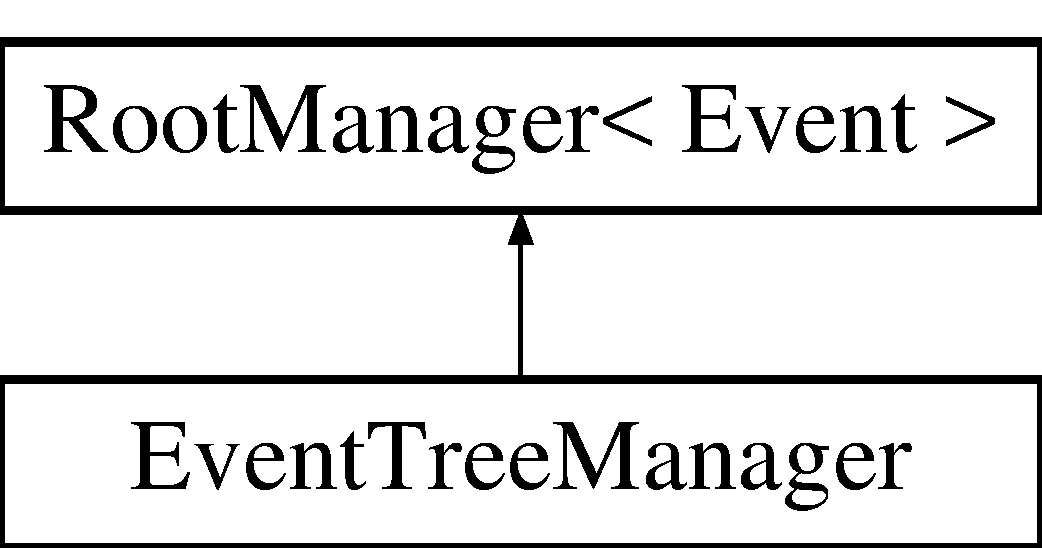
\includegraphics[height=2.000000cm]{class_event_tree_manager}
\end{center}
\end{figure}
\subsection*{Public Member Functions}
\begin{DoxyCompactItemize}
\item 
\hyperlink{class_event_tree_manager_a923f2a2c38074ddc0d6eb55091400a5f}{Event\+Tree\+Manager} (std\+::shared\+\_\+ptr$<$ const \hyperlink{class_config}{Config} $>$ config, const std\+::string outfile\+Name, const unsigned int n\+Readouts)
\begin{DoxyCompactList}\small\item\em Constructor. \end{DoxyCompactList}\item 
void \hyperlink{class_event_tree_manager_acabb2f6c8dd0e08375b4cf8bf2c148fd}{add} (std\+::unique\+\_\+ptr$<$ \hyperlink{class_event}{Event} $>$ event) final
\begin{DoxyCompactList}\small\item\em Adds an event to the tree, then destroys the event. \end{DoxyCompactList}\end{DoxyCompactItemize}
\subsection*{Private Member Functions}
\begin{DoxyCompactItemize}
\item 
void \hyperlink{class_event_tree_manager_a11cbe0078aeb3d0fe320bbeec335babc}{set\+Up\+Branches} ()
\begin{DoxyCompactList}\small\item\em Sets up the branches of the tree. \end{DoxyCompactList}\end{DoxyCompactItemize}
\subsection*{Private Attributes}
\begin{DoxyCompactItemize}
\item 
const unsigned int \hyperlink{class_event_tree_manager_ac0fce7275ef1c587302ff67e53ad5a77}{m\+\_\+n\+Readouts}
\begin{DoxyCompactList}\small\item\em The maximum number of T\+D\+Cs. \end{DoxyCompactList}\item 
const std\+::set$<$ unsigned int $>$ \hyperlink{class_event_tree_manager_aea70f1feef081fb124517ba8efc4087b}{m\+\_\+edge\+Matching\+Exclusions}
\begin{DoxyCompactList}\small\item\em Set to store edge matching exclusions. \end{DoxyCompactList}\item 
Bool\+\_\+t \hyperlink{class_event_tree_manager_a6e9b9bd6363f95fce295b19cb544ea83}{b\+\_\+is\+Complete} = false
\begin{DoxyCompactList}\small\item\em Branch Variable\+: Is event complete? \end{DoxyCompactList}\item 
Bool\+\_\+t \hyperlink{class_event_tree_manager_ab99e54a6c2d4c59bb073038649b3ae4f}{b\+\_\+was\+Dumped} = false
\begin{DoxyCompactList}\small\item\em Branch Variable\+: Was the event dumped? \end{DoxyCompactList}\item 
U\+Int\+\_\+t \hyperlink{class_event_tree_manager_a423068e1ef8766b602d5383bfe38494b}{b\+\_\+n\+Readouts} = 0
\begin{DoxyCompactList}\small\item\em Branch Variable\+: The number of Readouts (= n\+T\+DC chips used) \end{DoxyCompactList}\item 
U\+Int\+\_\+t $\ast$ \hyperlink{class_event_tree_manager_acad948110ea80051649765fdbed3fc91}{b\+\_\+chain\+ID} = nullptr
\begin{DoxyCompactList}\small\item\em Branch Variable \mbox{[}n\+Readouts\mbox{]}\+: Chain ID. \end{DoxyCompactList}\item 
U\+Int\+\_\+t $\ast$ \hyperlink{class_event_tree_manager_ab715e26f142e12ccd0e4ed6751959f0f}{b\+\_\+device\+ID} = nullptr
\begin{DoxyCompactList}\small\item\em Branch Variable \mbox{[}n\+Readouts\mbox{]}\+: Device ID. \end{DoxyCompactList}\item 
U\+Int\+\_\+t $\ast$ \hyperlink{class_event_tree_manager_a0e8cb571dd8ffe1295e9e31ce45c5d82}{b\+\_\+tdc\+ID} = nullptr
\begin{DoxyCompactList}\small\item\em Branch Variable \mbox{[}n\+Readouts\mbox{]}\+: T\+CD ID. \end{DoxyCompactList}\item 
U\+Int\+\_\+t $\ast$ \hyperlink{class_event_tree_manager_a3dea1a727165f6864be347642fc0728f}{b\+\_\+event\+ID} = nullptr
\begin{DoxyCompactList}\small\item\em Branch Variable \mbox{[}n\+Readouts\mbox{]}\+: \hyperlink{class_event}{Event} ID for each T\+DC. \end{DoxyCompactList}\item 
U\+Int\+\_\+t $\ast$ \hyperlink{class_event_tree_manager_a4953fdf79783fdd5c0b867af1dbd8f3d}{b\+\_\+bunch\+ID} = nullptr
\begin{DoxyCompactList}\small\item\em Branch Variable \mbox{[}n\+Readouts\mbox{]}\+: Bunch ID for each T\+DC. \end{DoxyCompactList}\item 
U\+Int\+\_\+t $\ast$ \hyperlink{class_event_tree_manager_acc8b0c67ad8e331ea9fc3f94a57d072b}{b\+\_\+roc\+Time} = nullptr
\begin{DoxyCompactList}\small\item\em Branch Variable \mbox{[}n\+Readouts\mbox{]}\+: R\+OC value for each T\+DC. \end{DoxyCompactList}\item 
U\+Int\+\_\+t $\ast$ \hyperlink{class_event_tree_manager_ac85cc79e72eaec4f7554a10e12e4d75a}{b\+\_\+n\+Headers} = nullptr
\begin{DoxyCompactList}\small\item\em Branch Variable \mbox{[}n\+Readouts\mbox{]}\+: Number for headers for each T\+DC. \end{DoxyCompactList}\item 
U\+Int\+\_\+t $\ast$ \hyperlink{class_event_tree_manager_ac32836178a53f00fe5417e533a0390f1}{b\+\_\+n\+Leading\+Edges} = nullptr
\begin{DoxyCompactList}\small\item\em Branch Variable \mbox{[}n\+Readouts\mbox{]}\+: Number for leading edges for each T\+DC. \end{DoxyCompactList}\item 
U\+Int\+\_\+t $\ast$ \hyperlink{class_event_tree_manager_aabb6a03aaab8095cb3e5e04d8389194a}{b\+\_\+n\+Trailing\+Edges} = nullptr
\begin{DoxyCompactList}\small\item\em Branch Variable \mbox{[}n\+Readouts\mbox{]}\+: Number for trailing edges for each T\+DC. \end{DoxyCompactList}\item 
U\+Int\+\_\+t $\ast$ \hyperlink{class_event_tree_manager_ae3d13f63577de75ec8a673ddb8686629}{b\+\_\+n\+Trailers} = nullptr
\begin{DoxyCompactList}\small\item\em Branch Variable \mbox{[}n\+Readouts\mbox{]}\+: Number for trailers for each T\+DC. \end{DoxyCompactList}\item 
U\+Int\+\_\+t $\ast$ \hyperlink{class_event_tree_manager_a7151f5beadcec7080e1b95f12e52a40a}{b\+\_\+word\+Count} = nullptr
\begin{DoxyCompactList}\small\item\em Branch Variable \mbox{[}n\+Readouts\mbox{]}\+: Word count for each T\+DC. \end{DoxyCompactList}\item 
U\+Int\+\_\+t \hyperlink{class_event_tree_manager_a050eedbaf401226c641f54b533cf8d01}{b\+\_\+n\+Edges} = 0
\begin{DoxyCompactList}\small\item\em Branch Variable\+: Total number of edges. \end{DoxyCompactList}\item 
U\+Int\+\_\+t \hyperlink{class_event_tree_manager_a7b7301d89e353ca96b42bcfb360c325e}{b\+\_\+n\+Hits} = 0
\begin{DoxyCompactList}\small\item\em Branch Variable\+: Total number of hits. \end{DoxyCompactList}\item 
U\+Int\+\_\+t $\ast$ \hyperlink{class_event_tree_manager_a663158889f41e6c32537aa698292e4ec}{b\+\_\+channel\+ID} = nullptr
\begin{DoxyCompactList}\small\item\em Branch Variable \mbox{[}n\+Hits\mbox{]}\+: Channel I\+Ds for each hit. \end{DoxyCompactList}\item 
U\+Int\+\_\+t $\ast$ \hyperlink{class_event_tree_manager_a4a117b0ff10078a9946096a868f243ce}{b\+\_\+leading\+Time} = nullptr
\begin{DoxyCompactList}\small\item\em Branch Variable \mbox{[}n\+Hits\mbox{]}\+: Leading time for each hit. \end{DoxyCompactList}\item 
U\+Int\+\_\+t $\ast$ \hyperlink{class_event_tree_manager_ad7533269c176ad00ec0fffe2afdf351a}{b\+\_\+trailing\+Time} = nullptr
\begin{DoxyCompactList}\small\item\em Branch Variable \mbox{[}n\+Hits\mbox{]}\+: Trailing time for each hit. \end{DoxyCompactList}\item 
U\+Int\+\_\+t $\ast$ \hyperlink{class_event_tree_manager_af2d628b1f5c54595b2f2b618b175af6f}{b\+\_\+leading\+Time\+Fine} = nullptr
\begin{DoxyCompactList}\small\item\em Branch Variable \mbox{[}n\+Hits\mbox{]}\+: Fine leading time for each hit. \end{DoxyCompactList}\item 
U\+Int\+\_\+t $\ast$ \hyperlink{class_event_tree_manager_a6c06cd342910a86ac1db079dfd7c5da2}{b\+\_\+trailing\+Time\+Fine} = nullptr
\begin{DoxyCompactList}\small\item\em Branch Variable \mbox{[}n\+Hits\mbox{]}\+: Fine trailing time for each hit. \end{DoxyCompactList}\item 
Int\+\_\+t $\ast$ \hyperlink{class_event_tree_manager_aa65fec5d7e3a3b3983730033a6a4a7b8}{b\+\_\+width} = nullptr
\begin{DoxyCompactList}\small\item\em Branch Variable \mbox{[}n\+Hits\mbox{]}\+: Width of signal. \end{DoxyCompactList}\end{DoxyCompactItemize}
\subsection*{Static Private Attributes}
\begin{DoxyCompactItemize}
\item 
static constexpr unsigned int \hyperlink{class_event_tree_manager_aab35ad52374d52149bde894c8af7a8c5}{s\+\_\+hits\+Max} = 1600
\begin{DoxyCompactList}\small\item\em Array size for hit branches. \end{DoxyCompactList}\end{DoxyCompactItemize}
\subsection*{Additional Inherited Members}


\subsection{Detailed Description}
Class which manages storage of \hyperlink{class_event}{Event} data in root file output. 

\subsection{Constructor \& Destructor Documentation}
\mbox{\Hypertarget{class_event_tree_manager_a923f2a2c38074ddc0d6eb55091400a5f}\label{class_event_tree_manager_a923f2a2c38074ddc0d6eb55091400a5f}} 
\index{Event\+Tree\+Manager@{Event\+Tree\+Manager}!Event\+Tree\+Manager@{Event\+Tree\+Manager}}
\index{Event\+Tree\+Manager@{Event\+Tree\+Manager}!Event\+Tree\+Manager@{Event\+Tree\+Manager}}
\subsubsection{\texorpdfstring{Event\+Tree\+Manager()}{EventTreeManager()}}
{\footnotesize\ttfamily Event\+Tree\+Manager\+::\+Event\+Tree\+Manager (\begin{DoxyParamCaption}\item[{std\+::shared\+\_\+ptr$<$ const \hyperlink{class_config}{Config} $>$}]{config,  }\item[{const std\+::string}]{outfile\+Name,  }\item[{const unsigned int}]{n\+Readouts }\end{DoxyParamCaption})}



Constructor. 


\begin{DoxyParams}{Parameters}
{\em config} & Ptr to program configuration \\
\hline
{\em outfile\+Name} & The desired output file name \\
\hline
{\em n\+Readouts} & Number of T\+D\+Cs present from config \\
\hline
\end{DoxyParams}


\subsection{Member Function Documentation}
\mbox{\Hypertarget{class_event_tree_manager_acabb2f6c8dd0e08375b4cf8bf2c148fd}\label{class_event_tree_manager_acabb2f6c8dd0e08375b4cf8bf2c148fd}} 
\index{Event\+Tree\+Manager@{Event\+Tree\+Manager}!add@{add}}
\index{add@{add}!Event\+Tree\+Manager@{Event\+Tree\+Manager}}
\subsubsection{\texorpdfstring{add()}{add()}}
{\footnotesize\ttfamily void Event\+Tree\+Manager\+::add (\begin{DoxyParamCaption}\item[{std\+::unique\+\_\+ptr$<$ \hyperlink{class_event}{Event} $>$}]{event }\end{DoxyParamCaption})\hspace{0.3cm}{\ttfamily [final]}, {\ttfamily [virtual]}}



Adds an event to the tree, then destroys the event. 

Overload of \hyperlink{class_root_manager}{Root\+Manager} add. 

Implements \hyperlink{class_root_manager_a2f05eb45d5eaee1f9f12e299395652fb}{Root\+Manager$<$ Event $>$}.

\mbox{\Hypertarget{class_event_tree_manager_a11cbe0078aeb3d0fe320bbeec335babc}\label{class_event_tree_manager_a11cbe0078aeb3d0fe320bbeec335babc}} 
\index{Event\+Tree\+Manager@{Event\+Tree\+Manager}!set\+Up\+Branches@{set\+Up\+Branches}}
\index{set\+Up\+Branches@{set\+Up\+Branches}!Event\+Tree\+Manager@{Event\+Tree\+Manager}}
\subsubsection{\texorpdfstring{set\+Up\+Branches()}{setUpBranches()}}
{\footnotesize\ttfamily void Event\+Tree\+Manager\+::set\+Up\+Branches (\begin{DoxyParamCaption}{ }\end{DoxyParamCaption})\hspace{0.3cm}{\ttfamily [private]}}



Sets up the branches of the tree. 



\subsection{Member Data Documentation}
\mbox{\Hypertarget{class_event_tree_manager_a4953fdf79783fdd5c0b867af1dbd8f3d}\label{class_event_tree_manager_a4953fdf79783fdd5c0b867af1dbd8f3d}} 
\index{Event\+Tree\+Manager@{Event\+Tree\+Manager}!b\+\_\+bunch\+ID@{b\+\_\+bunch\+ID}}
\index{b\+\_\+bunch\+ID@{b\+\_\+bunch\+ID}!Event\+Tree\+Manager@{Event\+Tree\+Manager}}
\subsubsection{\texorpdfstring{b\+\_\+bunch\+ID}{b\_bunchID}}
{\footnotesize\ttfamily U\+Int\+\_\+t$\ast$ Event\+Tree\+Manager\+::b\+\_\+bunch\+ID = nullptr\hspace{0.3cm}{\ttfamily [private]}}



Branch Variable \mbox{[}n\+Readouts\mbox{]}\+: Bunch ID for each T\+DC. 

\mbox{\Hypertarget{class_event_tree_manager_acad948110ea80051649765fdbed3fc91}\label{class_event_tree_manager_acad948110ea80051649765fdbed3fc91}} 
\index{Event\+Tree\+Manager@{Event\+Tree\+Manager}!b\+\_\+chain\+ID@{b\+\_\+chain\+ID}}
\index{b\+\_\+chain\+ID@{b\+\_\+chain\+ID}!Event\+Tree\+Manager@{Event\+Tree\+Manager}}
\subsubsection{\texorpdfstring{b\+\_\+chain\+ID}{b\_chainID}}
{\footnotesize\ttfamily U\+Int\+\_\+t$\ast$ Event\+Tree\+Manager\+::b\+\_\+chain\+ID = nullptr\hspace{0.3cm}{\ttfamily [private]}}



Branch Variable \mbox{[}n\+Readouts\mbox{]}\+: Chain ID. 

\mbox{\Hypertarget{class_event_tree_manager_a663158889f41e6c32537aa698292e4ec}\label{class_event_tree_manager_a663158889f41e6c32537aa698292e4ec}} 
\index{Event\+Tree\+Manager@{Event\+Tree\+Manager}!b\+\_\+channel\+ID@{b\+\_\+channel\+ID}}
\index{b\+\_\+channel\+ID@{b\+\_\+channel\+ID}!Event\+Tree\+Manager@{Event\+Tree\+Manager}}
\subsubsection{\texorpdfstring{b\+\_\+channel\+ID}{b\_channelID}}
{\footnotesize\ttfamily U\+Int\+\_\+t$\ast$ Event\+Tree\+Manager\+::b\+\_\+channel\+ID = nullptr\hspace{0.3cm}{\ttfamily [private]}}



Branch Variable \mbox{[}n\+Hits\mbox{]}\+: Channel I\+Ds for each hit. 

\mbox{\Hypertarget{class_event_tree_manager_ab715e26f142e12ccd0e4ed6751959f0f}\label{class_event_tree_manager_ab715e26f142e12ccd0e4ed6751959f0f}} 
\index{Event\+Tree\+Manager@{Event\+Tree\+Manager}!b\+\_\+device\+ID@{b\+\_\+device\+ID}}
\index{b\+\_\+device\+ID@{b\+\_\+device\+ID}!Event\+Tree\+Manager@{Event\+Tree\+Manager}}
\subsubsection{\texorpdfstring{b\+\_\+device\+ID}{b\_deviceID}}
{\footnotesize\ttfamily U\+Int\+\_\+t$\ast$ Event\+Tree\+Manager\+::b\+\_\+device\+ID = nullptr\hspace{0.3cm}{\ttfamily [private]}}



Branch Variable \mbox{[}n\+Readouts\mbox{]}\+: Device ID. 

\mbox{\Hypertarget{class_event_tree_manager_a3dea1a727165f6864be347642fc0728f}\label{class_event_tree_manager_a3dea1a727165f6864be347642fc0728f}} 
\index{Event\+Tree\+Manager@{Event\+Tree\+Manager}!b\+\_\+event\+ID@{b\+\_\+event\+ID}}
\index{b\+\_\+event\+ID@{b\+\_\+event\+ID}!Event\+Tree\+Manager@{Event\+Tree\+Manager}}
\subsubsection{\texorpdfstring{b\+\_\+event\+ID}{b\_eventID}}
{\footnotesize\ttfamily U\+Int\+\_\+t$\ast$ Event\+Tree\+Manager\+::b\+\_\+event\+ID = nullptr\hspace{0.3cm}{\ttfamily [private]}}



Branch Variable \mbox{[}n\+Readouts\mbox{]}\+: \hyperlink{class_event}{Event} ID for each T\+DC. 

\mbox{\Hypertarget{class_event_tree_manager_a6e9b9bd6363f95fce295b19cb544ea83}\label{class_event_tree_manager_a6e9b9bd6363f95fce295b19cb544ea83}} 
\index{Event\+Tree\+Manager@{Event\+Tree\+Manager}!b\+\_\+is\+Complete@{b\+\_\+is\+Complete}}
\index{b\+\_\+is\+Complete@{b\+\_\+is\+Complete}!Event\+Tree\+Manager@{Event\+Tree\+Manager}}
\subsubsection{\texorpdfstring{b\+\_\+is\+Complete}{b\_isComplete}}
{\footnotesize\ttfamily Bool\+\_\+t Event\+Tree\+Manager\+::b\+\_\+is\+Complete = false\hspace{0.3cm}{\ttfamily [private]}}



Branch Variable\+: Is event complete? 

\mbox{\Hypertarget{class_event_tree_manager_a4a117b0ff10078a9946096a868f243ce}\label{class_event_tree_manager_a4a117b0ff10078a9946096a868f243ce}} 
\index{Event\+Tree\+Manager@{Event\+Tree\+Manager}!b\+\_\+leading\+Time@{b\+\_\+leading\+Time}}
\index{b\+\_\+leading\+Time@{b\+\_\+leading\+Time}!Event\+Tree\+Manager@{Event\+Tree\+Manager}}
\subsubsection{\texorpdfstring{b\+\_\+leading\+Time}{b\_leadingTime}}
{\footnotesize\ttfamily U\+Int\+\_\+t$\ast$ Event\+Tree\+Manager\+::b\+\_\+leading\+Time = nullptr\hspace{0.3cm}{\ttfamily [private]}}



Branch Variable \mbox{[}n\+Hits\mbox{]}\+: Leading time for each hit. 

\mbox{\Hypertarget{class_event_tree_manager_af2d628b1f5c54595b2f2b618b175af6f}\label{class_event_tree_manager_af2d628b1f5c54595b2f2b618b175af6f}} 
\index{Event\+Tree\+Manager@{Event\+Tree\+Manager}!b\+\_\+leading\+Time\+Fine@{b\+\_\+leading\+Time\+Fine}}
\index{b\+\_\+leading\+Time\+Fine@{b\+\_\+leading\+Time\+Fine}!Event\+Tree\+Manager@{Event\+Tree\+Manager}}
\subsubsection{\texorpdfstring{b\+\_\+leading\+Time\+Fine}{b\_leadingTimeFine}}
{\footnotesize\ttfamily U\+Int\+\_\+t$\ast$ Event\+Tree\+Manager\+::b\+\_\+leading\+Time\+Fine = nullptr\hspace{0.3cm}{\ttfamily [private]}}



Branch Variable \mbox{[}n\+Hits\mbox{]}\+: Fine leading time for each hit. 

\mbox{\Hypertarget{class_event_tree_manager_a050eedbaf401226c641f54b533cf8d01}\label{class_event_tree_manager_a050eedbaf401226c641f54b533cf8d01}} 
\index{Event\+Tree\+Manager@{Event\+Tree\+Manager}!b\+\_\+n\+Edges@{b\+\_\+n\+Edges}}
\index{b\+\_\+n\+Edges@{b\+\_\+n\+Edges}!Event\+Tree\+Manager@{Event\+Tree\+Manager}}
\subsubsection{\texorpdfstring{b\+\_\+n\+Edges}{b\_nEdges}}
{\footnotesize\ttfamily U\+Int\+\_\+t Event\+Tree\+Manager\+::b\+\_\+n\+Edges = 0\hspace{0.3cm}{\ttfamily [private]}}



Branch Variable\+: Total number of edges. 

\mbox{\Hypertarget{class_event_tree_manager_ac85cc79e72eaec4f7554a10e12e4d75a}\label{class_event_tree_manager_ac85cc79e72eaec4f7554a10e12e4d75a}} 
\index{Event\+Tree\+Manager@{Event\+Tree\+Manager}!b\+\_\+n\+Headers@{b\+\_\+n\+Headers}}
\index{b\+\_\+n\+Headers@{b\+\_\+n\+Headers}!Event\+Tree\+Manager@{Event\+Tree\+Manager}}
\subsubsection{\texorpdfstring{b\+\_\+n\+Headers}{b\_nHeaders}}
{\footnotesize\ttfamily U\+Int\+\_\+t$\ast$ Event\+Tree\+Manager\+::b\+\_\+n\+Headers = nullptr\hspace{0.3cm}{\ttfamily [private]}}



Branch Variable \mbox{[}n\+Readouts\mbox{]}\+: Number for headers for each T\+DC. 

\mbox{\Hypertarget{class_event_tree_manager_a7b7301d89e353ca96b42bcfb360c325e}\label{class_event_tree_manager_a7b7301d89e353ca96b42bcfb360c325e}} 
\index{Event\+Tree\+Manager@{Event\+Tree\+Manager}!b\+\_\+n\+Hits@{b\+\_\+n\+Hits}}
\index{b\+\_\+n\+Hits@{b\+\_\+n\+Hits}!Event\+Tree\+Manager@{Event\+Tree\+Manager}}
\subsubsection{\texorpdfstring{b\+\_\+n\+Hits}{b\_nHits}}
{\footnotesize\ttfamily U\+Int\+\_\+t Event\+Tree\+Manager\+::b\+\_\+n\+Hits = 0\hspace{0.3cm}{\ttfamily [private]}}



Branch Variable\+: Total number of hits. 

\mbox{\Hypertarget{class_event_tree_manager_ac32836178a53f00fe5417e533a0390f1}\label{class_event_tree_manager_ac32836178a53f00fe5417e533a0390f1}} 
\index{Event\+Tree\+Manager@{Event\+Tree\+Manager}!b\+\_\+n\+Leading\+Edges@{b\+\_\+n\+Leading\+Edges}}
\index{b\+\_\+n\+Leading\+Edges@{b\+\_\+n\+Leading\+Edges}!Event\+Tree\+Manager@{Event\+Tree\+Manager}}
\subsubsection{\texorpdfstring{b\+\_\+n\+Leading\+Edges}{b\_nLeadingEdges}}
{\footnotesize\ttfamily U\+Int\+\_\+t$\ast$ Event\+Tree\+Manager\+::b\+\_\+n\+Leading\+Edges = nullptr\hspace{0.3cm}{\ttfamily [private]}}



Branch Variable \mbox{[}n\+Readouts\mbox{]}\+: Number for leading edges for each T\+DC. 

\mbox{\Hypertarget{class_event_tree_manager_a423068e1ef8766b602d5383bfe38494b}\label{class_event_tree_manager_a423068e1ef8766b602d5383bfe38494b}} 
\index{Event\+Tree\+Manager@{Event\+Tree\+Manager}!b\+\_\+n\+Readouts@{b\+\_\+n\+Readouts}}
\index{b\+\_\+n\+Readouts@{b\+\_\+n\+Readouts}!Event\+Tree\+Manager@{Event\+Tree\+Manager}}
\subsubsection{\texorpdfstring{b\+\_\+n\+Readouts}{b\_nReadouts}}
{\footnotesize\ttfamily U\+Int\+\_\+t Event\+Tree\+Manager\+::b\+\_\+n\+Readouts = 0\hspace{0.3cm}{\ttfamily [private]}}



Branch Variable\+: The number of Readouts (= n\+T\+DC chips used) 

\mbox{\Hypertarget{class_event_tree_manager_ae3d13f63577de75ec8a673ddb8686629}\label{class_event_tree_manager_ae3d13f63577de75ec8a673ddb8686629}} 
\index{Event\+Tree\+Manager@{Event\+Tree\+Manager}!b\+\_\+n\+Trailers@{b\+\_\+n\+Trailers}}
\index{b\+\_\+n\+Trailers@{b\+\_\+n\+Trailers}!Event\+Tree\+Manager@{Event\+Tree\+Manager}}
\subsubsection{\texorpdfstring{b\+\_\+n\+Trailers}{b\_nTrailers}}
{\footnotesize\ttfamily U\+Int\+\_\+t$\ast$ Event\+Tree\+Manager\+::b\+\_\+n\+Trailers = nullptr\hspace{0.3cm}{\ttfamily [private]}}



Branch Variable \mbox{[}n\+Readouts\mbox{]}\+: Number for trailers for each T\+DC. 

\mbox{\Hypertarget{class_event_tree_manager_aabb6a03aaab8095cb3e5e04d8389194a}\label{class_event_tree_manager_aabb6a03aaab8095cb3e5e04d8389194a}} 
\index{Event\+Tree\+Manager@{Event\+Tree\+Manager}!b\+\_\+n\+Trailing\+Edges@{b\+\_\+n\+Trailing\+Edges}}
\index{b\+\_\+n\+Trailing\+Edges@{b\+\_\+n\+Trailing\+Edges}!Event\+Tree\+Manager@{Event\+Tree\+Manager}}
\subsubsection{\texorpdfstring{b\+\_\+n\+Trailing\+Edges}{b\_nTrailingEdges}}
{\footnotesize\ttfamily U\+Int\+\_\+t$\ast$ Event\+Tree\+Manager\+::b\+\_\+n\+Trailing\+Edges = nullptr\hspace{0.3cm}{\ttfamily [private]}}



Branch Variable \mbox{[}n\+Readouts\mbox{]}\+: Number for trailing edges for each T\+DC. 

\mbox{\Hypertarget{class_event_tree_manager_acc8b0c67ad8e331ea9fc3f94a57d072b}\label{class_event_tree_manager_acc8b0c67ad8e331ea9fc3f94a57d072b}} 
\index{Event\+Tree\+Manager@{Event\+Tree\+Manager}!b\+\_\+roc\+Time@{b\+\_\+roc\+Time}}
\index{b\+\_\+roc\+Time@{b\+\_\+roc\+Time}!Event\+Tree\+Manager@{Event\+Tree\+Manager}}
\subsubsection{\texorpdfstring{b\+\_\+roc\+Time}{b\_rocTime}}
{\footnotesize\ttfamily U\+Int\+\_\+t$\ast$ Event\+Tree\+Manager\+::b\+\_\+roc\+Time = nullptr\hspace{0.3cm}{\ttfamily [private]}}



Branch Variable \mbox{[}n\+Readouts\mbox{]}\+: R\+OC value for each T\+DC. 

\mbox{\Hypertarget{class_event_tree_manager_a0e8cb571dd8ffe1295e9e31ce45c5d82}\label{class_event_tree_manager_a0e8cb571dd8ffe1295e9e31ce45c5d82}} 
\index{Event\+Tree\+Manager@{Event\+Tree\+Manager}!b\+\_\+tdc\+ID@{b\+\_\+tdc\+ID}}
\index{b\+\_\+tdc\+ID@{b\+\_\+tdc\+ID}!Event\+Tree\+Manager@{Event\+Tree\+Manager}}
\subsubsection{\texorpdfstring{b\+\_\+tdc\+ID}{b\_tdcID}}
{\footnotesize\ttfamily U\+Int\+\_\+t$\ast$ Event\+Tree\+Manager\+::b\+\_\+tdc\+ID = nullptr\hspace{0.3cm}{\ttfamily [private]}}



Branch Variable \mbox{[}n\+Readouts\mbox{]}\+: T\+CD ID. 

\mbox{\Hypertarget{class_event_tree_manager_ad7533269c176ad00ec0fffe2afdf351a}\label{class_event_tree_manager_ad7533269c176ad00ec0fffe2afdf351a}} 
\index{Event\+Tree\+Manager@{Event\+Tree\+Manager}!b\+\_\+trailing\+Time@{b\+\_\+trailing\+Time}}
\index{b\+\_\+trailing\+Time@{b\+\_\+trailing\+Time}!Event\+Tree\+Manager@{Event\+Tree\+Manager}}
\subsubsection{\texorpdfstring{b\+\_\+trailing\+Time}{b\_trailingTime}}
{\footnotesize\ttfamily U\+Int\+\_\+t$\ast$ Event\+Tree\+Manager\+::b\+\_\+trailing\+Time = nullptr\hspace{0.3cm}{\ttfamily [private]}}



Branch Variable \mbox{[}n\+Hits\mbox{]}\+: Trailing time for each hit. 

\mbox{\Hypertarget{class_event_tree_manager_a6c06cd342910a86ac1db079dfd7c5da2}\label{class_event_tree_manager_a6c06cd342910a86ac1db079dfd7c5da2}} 
\index{Event\+Tree\+Manager@{Event\+Tree\+Manager}!b\+\_\+trailing\+Time\+Fine@{b\+\_\+trailing\+Time\+Fine}}
\index{b\+\_\+trailing\+Time\+Fine@{b\+\_\+trailing\+Time\+Fine}!Event\+Tree\+Manager@{Event\+Tree\+Manager}}
\subsubsection{\texorpdfstring{b\+\_\+trailing\+Time\+Fine}{b\_trailingTimeFine}}
{\footnotesize\ttfamily U\+Int\+\_\+t$\ast$ Event\+Tree\+Manager\+::b\+\_\+trailing\+Time\+Fine = nullptr\hspace{0.3cm}{\ttfamily [private]}}



Branch Variable \mbox{[}n\+Hits\mbox{]}\+: Fine trailing time for each hit. 

\mbox{\Hypertarget{class_event_tree_manager_ab99e54a6c2d4c59bb073038649b3ae4f}\label{class_event_tree_manager_ab99e54a6c2d4c59bb073038649b3ae4f}} 
\index{Event\+Tree\+Manager@{Event\+Tree\+Manager}!b\+\_\+was\+Dumped@{b\+\_\+was\+Dumped}}
\index{b\+\_\+was\+Dumped@{b\+\_\+was\+Dumped}!Event\+Tree\+Manager@{Event\+Tree\+Manager}}
\subsubsection{\texorpdfstring{b\+\_\+was\+Dumped}{b\_wasDumped}}
{\footnotesize\ttfamily Bool\+\_\+t Event\+Tree\+Manager\+::b\+\_\+was\+Dumped = false\hspace{0.3cm}{\ttfamily [private]}}



Branch Variable\+: Was the event dumped? 

\mbox{\Hypertarget{class_event_tree_manager_aa65fec5d7e3a3b3983730033a6a4a7b8}\label{class_event_tree_manager_aa65fec5d7e3a3b3983730033a6a4a7b8}} 
\index{Event\+Tree\+Manager@{Event\+Tree\+Manager}!b\+\_\+width@{b\+\_\+width}}
\index{b\+\_\+width@{b\+\_\+width}!Event\+Tree\+Manager@{Event\+Tree\+Manager}}
\subsubsection{\texorpdfstring{b\+\_\+width}{b\_width}}
{\footnotesize\ttfamily Int\+\_\+t$\ast$ Event\+Tree\+Manager\+::b\+\_\+width = nullptr\hspace{0.3cm}{\ttfamily [private]}}



Branch Variable \mbox{[}n\+Hits\mbox{]}\+: Width of signal. 

\mbox{\Hypertarget{class_event_tree_manager_a7151f5beadcec7080e1b95f12e52a40a}\label{class_event_tree_manager_a7151f5beadcec7080e1b95f12e52a40a}} 
\index{Event\+Tree\+Manager@{Event\+Tree\+Manager}!b\+\_\+word\+Count@{b\+\_\+word\+Count}}
\index{b\+\_\+word\+Count@{b\+\_\+word\+Count}!Event\+Tree\+Manager@{Event\+Tree\+Manager}}
\subsubsection{\texorpdfstring{b\+\_\+word\+Count}{b\_wordCount}}
{\footnotesize\ttfamily U\+Int\+\_\+t$\ast$ Event\+Tree\+Manager\+::b\+\_\+word\+Count = nullptr\hspace{0.3cm}{\ttfamily [private]}}



Branch Variable \mbox{[}n\+Readouts\mbox{]}\+: Word count for each T\+DC. 

\mbox{\Hypertarget{class_event_tree_manager_aea70f1feef081fb124517ba8efc4087b}\label{class_event_tree_manager_aea70f1feef081fb124517ba8efc4087b}} 
\index{Event\+Tree\+Manager@{Event\+Tree\+Manager}!m\+\_\+edge\+Matching\+Exclusions@{m\+\_\+edge\+Matching\+Exclusions}}
\index{m\+\_\+edge\+Matching\+Exclusions@{m\+\_\+edge\+Matching\+Exclusions}!Event\+Tree\+Manager@{Event\+Tree\+Manager}}
\subsubsection{\texorpdfstring{m\+\_\+edge\+Matching\+Exclusions}{m\_edgeMatchingExclusions}}
{\footnotesize\ttfamily const std\+::set$<$unsigned int$>$ Event\+Tree\+Manager\+::m\+\_\+edge\+Matching\+Exclusions\hspace{0.3cm}{\ttfamily [private]}}



Set to store edge matching exclusions. 

\mbox{\Hypertarget{class_event_tree_manager_ac0fce7275ef1c587302ff67e53ad5a77}\label{class_event_tree_manager_ac0fce7275ef1c587302ff67e53ad5a77}} 
\index{Event\+Tree\+Manager@{Event\+Tree\+Manager}!m\+\_\+n\+Readouts@{m\+\_\+n\+Readouts}}
\index{m\+\_\+n\+Readouts@{m\+\_\+n\+Readouts}!Event\+Tree\+Manager@{Event\+Tree\+Manager}}
\subsubsection{\texorpdfstring{m\+\_\+n\+Readouts}{m\_nReadouts}}
{\footnotesize\ttfamily const unsigned int Event\+Tree\+Manager\+::m\+\_\+n\+Readouts\hspace{0.3cm}{\ttfamily [private]}}



The maximum number of T\+D\+Cs. 

\mbox{\Hypertarget{class_event_tree_manager_aab35ad52374d52149bde894c8af7a8c5}\label{class_event_tree_manager_aab35ad52374d52149bde894c8af7a8c5}} 
\index{Event\+Tree\+Manager@{Event\+Tree\+Manager}!s\+\_\+hits\+Max@{s\+\_\+hits\+Max}}
\index{s\+\_\+hits\+Max@{s\+\_\+hits\+Max}!Event\+Tree\+Manager@{Event\+Tree\+Manager}}
\subsubsection{\texorpdfstring{s\+\_\+hits\+Max}{s\_hitsMax}}
{\footnotesize\ttfamily constexpr unsigned int Event\+Tree\+Manager\+::s\+\_\+hits\+Max = 1600\hspace{0.3cm}{\ttfamily [static]}, {\ttfamily [private]}}



Array size for hit branches. 



The documentation for this class was generated from the following files\+:\begin{DoxyCompactItemize}
\item 
Root/inc/\hyperlink{_event_tree_manager_8hpp}{Event\+Tree\+Manager.\+hpp}\item 
Root/src/\hyperlink{_event_tree_manager_8cpp}{Event\+Tree\+Manager.\+cpp}\end{DoxyCompactItemize}

\hypertarget{class_file_reader}{}\section{File\+Reader Class Reference}
\label{class_file_reader}\index{File\+Reader@{File\+Reader}}


Read files and outputs word bundles.  




{\ttfamily \#include $<$File\+Reader.\+hpp$>$}

\subsection*{Public Member Functions}
\begin{DoxyCompactItemize}
\item 
\hyperlink{class_file_reader_a3be44012f3dc81ad7943b1012b64e52d}{File\+Reader} (const std\+::list$<$ unsigned int $>$ \&readout\+Board\+List, std\+::array$<$ std\+::shared\+\_\+ptr$<$ \hyperlink{class_file_reader_ac755c1e271610c2c12a7fc5b55cc048b}{bundle\+Buffer} $>$, 4 $>$)
\begin{DoxyCompactList}\small\item\em Constructor. \end{DoxyCompactList}\item 
void \hyperlink{class_file_reader_a5d487d37857d537ace41c31d6594ef3a}{stage\+Files} (const std\+::vector$<$ std\+::string $>$ \&files)
\begin{DoxyCompactList}\small\item\em Stages files to be read out together. \end{DoxyCompactList}\item 
bool \hyperlink{class_file_reader_a58b80f2c9c2ec8381527bdfca1008007}{have\+Files\+Expired} () const
\begin{DoxyCompactList}\small\item\em Checks if all files have finished being read. \end{DoxyCompactList}\item 
void \hyperlink{class_file_reader_a478ed77f1b8f76e15cb2faa8964a26e6}{run\+Processing\+Loops} (const unsigned int n\+Loops)
\begin{DoxyCompactList}\small\item\em Reads n\+Loops data blocks from each staged file. \end{DoxyCompactList}\end{DoxyCompactItemize}
\subsection*{Private Types}
\begin{DoxyCompactItemize}
\item 
using \hyperlink{class_file_reader_ac755c1e271610c2c12a7fc5b55cc048b}{bundle\+Buffer} = \hyperlink{class_thread_safe_queue}{Thread\+Safe\+Queue}$<$ std\+::unique\+\_\+ptr$<$ \hyperlink{class_word_bundle}{Word\+Bundle} $>$ $>$
\item 
using \hyperlink{class_file_reader_a7fb625dc45cee3256d37cc19c65cad86}{bundle\+Workspace} = std\+::array$<$ std\+::unique\+\_\+ptr$<$ \hyperlink{class_word_bundle}{Word\+Bundle} $>$, 4 $>$
\end{DoxyCompactItemize}
\subsection*{Private Member Functions}
\begin{DoxyCompactItemize}
\item 
void \hyperlink{class_file_reader_a3404694daef538fdd001a3e2ae898fb8}{add\+File} (const std\+::string \&file\+Path)
\begin{DoxyCompactList}\small\item\em Adds a file to be read out. \end{DoxyCompactList}\item 
void \hyperlink{class_file_reader_a381cceb460883f24a8113333ae1bf5bb}{stage\+Next\+File} (const unsigned int readout\+Board\+ID)
\begin{DoxyCompactList}\small\item\em Stages a new file. \end{DoxyCompactList}\item 
void \hyperlink{class_file_reader_a98606ec7d315f1ed6f90c531df0d09f9}{run\+Processing\+Loop} ()
\begin{DoxyCompactList}\small\item\em Reads a single data block from each file. \end{DoxyCompactList}\item 
unsigned int \hyperlink{class_file_reader_a94181d78b29ebacf2a4b3b3cd03a6750}{read\+Header\+Line} (std\+::unique\+\_\+ptr$<$ std\+::ifstream $>$ \&input\+Data)
\begin{DoxyCompactList}\small\item\em Reads a header line from the passed stream. \end{DoxyCompactList}\item 
bool \hyperlink{class_file_reader_ac3938817d6fd8b2d90ac479e323bdc03}{is\+N\+Data\+Bytes\+Valid} (const unsigned int board\+ID, std\+::unique\+\_\+ptr$<$ std\+::ifstream $>$ \&input\+Data, const unsigned int n\+Data\+Bytes)
\begin{DoxyCompactList}\small\item\em Checks if a number of bytes is valid, and takes action if not. \end{DoxyCompactList}\item 
std\+::array$<$ unsigned int, 4 $>$ \hyperlink{class_file_reader_ac578b683eba751027766a2c30f03a28b}{read\+Data\+Block} (std\+::unique\+\_\+ptr$<$ std\+::ifstream $>$ \&input\+Data)
\begin{DoxyCompactList}\small\item\em Reads a data block line from the passed stream. \end{DoxyCompactList}\end{DoxyCompactItemize}
\subsection*{Private Attributes}
\begin{DoxyCompactItemize}
\item 
std\+::map$<$ unsigned int, std\+::list$<$ \hyperlink{class_input_file}{Input\+File} $>$ $>$ \hyperlink{class_file_reader_a8b144dccc96fcc95e43a96a300341855}{m\+\_\+input\+Files}
\begin{DoxyCompactList}\small\item\em Input file storage. \end{DoxyCompactList}\item 
std\+::map$<$ unsigned int, std\+::unique\+\_\+ptr$<$ std\+::ifstream $>$ $>$ \hyperlink{class_file_reader_af7ac8567ed5b1fa022a8f98099e23f43}{m\+\_\+input\+Streams}
\begin{DoxyCompactList}\small\item\em Vector of input streams. \end{DoxyCompactList}\item 
std\+::unordered\+\_\+map$<$ unsigned int, unsigned int $>$ \hyperlink{class_file_reader_a2d560dd766f6866a1c11cc44e059c246}{m\+\_\+file\+Lengths}
\begin{DoxyCompactList}\small\item\em Map to store file lengths. \end{DoxyCompactList}\item 
std\+::unordered\+\_\+map$<$ unsigned int, \hyperlink{class_file_reader_a7fb625dc45cee3256d37cc19c65cad86}{bundle\+Workspace} $>$ \hyperlink{class_file_reader_aa04e6f9a40c9186cae2c89352e75d69c}{m\+\_\+bundle\+Workspaces}
\begin{DoxyCompactList}\small\item\em Map of pointers used to create Word\+Bundles. \end{DoxyCompactList}\item 
std\+::array$<$ std\+::shared\+\_\+ptr$<$ \hyperlink{class_file_reader_ac755c1e271610c2c12a7fc5b55cc048b}{bundle\+Buffer} $>$, 4 $>$ \hyperlink{class_file_reader_a038d1362d7e0458b3450ab8584eab688}{m\+\_\+word\+Bundle\+Buffers}
\begin{DoxyCompactList}\small\item\em Pointers to shared \hyperlink{class_word_bundle}{Word\+Bundle} buffers. \end{DoxyCompactList}\item 
const std\+::set$<$ unsigned int $>$ \hyperlink{class_file_reader_a7a0bb5e7cb117f6a415f005665893509}{filler\+Words} = \{ 0x\+A0\+A0\+A0\+A0, 0x\+B0\+B0\+B0\+B0, 0x\+C0\+C0\+C0\+C0, 0x\+D0\+D0\+D0\+D0 \}
\end{DoxyCompactItemize}


\subsection{Detailed Description}
Read files and outputs word bundles. 

\subsection{Member Typedef Documentation}
\mbox{\Hypertarget{class_file_reader_ac755c1e271610c2c12a7fc5b55cc048b}\label{class_file_reader_ac755c1e271610c2c12a7fc5b55cc048b}} 
\index{File\+Reader@{File\+Reader}!bundle\+Buffer@{bundle\+Buffer}}
\index{bundle\+Buffer@{bundle\+Buffer}!File\+Reader@{File\+Reader}}
\subsubsection{\texorpdfstring{bundle\+Buffer}{bundleBuffer}}
{\footnotesize\ttfamily using \hyperlink{class_file_reader_ac755c1e271610c2c12a7fc5b55cc048b}{File\+Reader\+::bundle\+Buffer} =  \hyperlink{class_thread_safe_queue}{Thread\+Safe\+Queue}$<$ std\+::unique\+\_\+ptr$<$\hyperlink{class_word_bundle}{Word\+Bundle}$>$ $>$\hspace{0.3cm}{\ttfamily [private]}}

\mbox{\Hypertarget{class_file_reader_a7fb625dc45cee3256d37cc19c65cad86}\label{class_file_reader_a7fb625dc45cee3256d37cc19c65cad86}} 
\index{File\+Reader@{File\+Reader}!bundle\+Workspace@{bundle\+Workspace}}
\index{bundle\+Workspace@{bundle\+Workspace}!File\+Reader@{File\+Reader}}
\subsubsection{\texorpdfstring{bundle\+Workspace}{bundleWorkspace}}
{\footnotesize\ttfamily using \hyperlink{class_file_reader_a7fb625dc45cee3256d37cc19c65cad86}{File\+Reader\+::bundle\+Workspace} =  std\+::array$<$ std\+::unique\+\_\+ptr$<$\hyperlink{class_word_bundle}{Word\+Bundle}$>$, 4$>$\hspace{0.3cm}{\ttfamily [private]}}



\subsection{Constructor \& Destructor Documentation}
\mbox{\Hypertarget{class_file_reader_a3be44012f3dc81ad7943b1012b64e52d}\label{class_file_reader_a3be44012f3dc81ad7943b1012b64e52d}} 
\index{File\+Reader@{File\+Reader}!File\+Reader@{File\+Reader}}
\index{File\+Reader@{File\+Reader}!File\+Reader@{File\+Reader}}
\subsubsection{\texorpdfstring{File\+Reader()}{FileReader()}}
{\footnotesize\ttfamily File\+Reader\+::\+File\+Reader (\begin{DoxyParamCaption}\item[{const std\+::list$<$ unsigned int $>$ \&}]{readout\+Board\+List,  }\item[{std\+::array$<$ std\+::shared\+\_\+ptr$<$ \hyperlink{class_file_reader_ac755c1e271610c2c12a7fc5b55cc048b}{bundle\+Buffer} $>$, 4 $>$}]{word\+Bundle\+Buffers }\end{DoxyParamCaption})}



Constructor. 


\begin{DoxyParams}{Parameters}
{\em readout\+Board\+List} & List of readout boards present \\
\hline
{\em word\+Bundle\+Buffers} & Shared Pointer to \hyperlink{class_word_bundle}{Word\+Bundle} buffers \\
\hline
\end{DoxyParams}


\subsection{Member Function Documentation}
\mbox{\Hypertarget{class_file_reader_a3404694daef538fdd001a3e2ae898fb8}\label{class_file_reader_a3404694daef538fdd001a3e2ae898fb8}} 
\index{File\+Reader@{File\+Reader}!add\+File@{add\+File}}
\index{add\+File@{add\+File}!File\+Reader@{File\+Reader}}
\subsubsection{\texorpdfstring{add\+File()}{addFile()}}
{\footnotesize\ttfamily void File\+Reader\+::add\+File (\begin{DoxyParamCaption}\item[{const std\+::string \&}]{file\+Path }\end{DoxyParamCaption})\hspace{0.3cm}{\ttfamily [private]}}



Adds a file to be read out. 


\begin{DoxyParams}{Parameters}
{\em file\+Path} & Path fo the file to add \\
\hline
\end{DoxyParams}
\mbox{\Hypertarget{class_file_reader_a58b80f2c9c2ec8381527bdfca1008007}\label{class_file_reader_a58b80f2c9c2ec8381527bdfca1008007}} 
\index{File\+Reader@{File\+Reader}!have\+Files\+Expired@{have\+Files\+Expired}}
\index{have\+Files\+Expired@{have\+Files\+Expired}!File\+Reader@{File\+Reader}}
\subsubsection{\texorpdfstring{have\+Files\+Expired()}{haveFilesExpired()}}
{\footnotesize\ttfamily bool File\+Reader\+::have\+Files\+Expired (\begin{DoxyParamCaption}{ }\end{DoxyParamCaption}) const\hspace{0.3cm}{\ttfamily [inline]}}



Checks if all files have finished being read. 

\mbox{\Hypertarget{class_file_reader_ac3938817d6fd8b2d90ac479e323bdc03}\label{class_file_reader_ac3938817d6fd8b2d90ac479e323bdc03}} 
\index{File\+Reader@{File\+Reader}!is\+N\+Data\+Bytes\+Valid@{is\+N\+Data\+Bytes\+Valid}}
\index{is\+N\+Data\+Bytes\+Valid@{is\+N\+Data\+Bytes\+Valid}!File\+Reader@{File\+Reader}}
\subsubsection{\texorpdfstring{is\+N\+Data\+Bytes\+Valid()}{isNDataBytesValid()}}
{\footnotesize\ttfamily bool File\+Reader\+::is\+N\+Data\+Bytes\+Valid (\begin{DoxyParamCaption}\item[{const unsigned int}]{board\+ID,  }\item[{std\+::unique\+\_\+ptr$<$ std\+::ifstream $>$ \&}]{input\+Data,  }\item[{const unsigned int}]{n\+Data\+Bytes }\end{DoxyParamCaption})\hspace{0.3cm}{\ttfamily [inline]}, {\ttfamily [private]}}



Checks if a number of bytes is valid, and takes action if not. 


\begin{DoxyParams}{Parameters}
{\em input\+Data} & Stream n\+Data\+Bytes was read from \\
\hline
\end{DoxyParams}
\mbox{\Hypertarget{class_file_reader_ac578b683eba751027766a2c30f03a28b}\label{class_file_reader_ac578b683eba751027766a2c30f03a28b}} 
\index{File\+Reader@{File\+Reader}!read\+Data\+Block@{read\+Data\+Block}}
\index{read\+Data\+Block@{read\+Data\+Block}!File\+Reader@{File\+Reader}}
\subsubsection{\texorpdfstring{read\+Data\+Block()}{readDataBlock()}}
{\footnotesize\ttfamily std\+::array$<$ unsigned int, 4 $>$ File\+Reader\+::read\+Data\+Block (\begin{DoxyParamCaption}\item[{std\+::unique\+\_\+ptr$<$ std\+::ifstream $>$ \&}]{input\+Data }\end{DoxyParamCaption})\hspace{0.3cm}{\ttfamily [inline]}, {\ttfamily [private]}}



Reads a data block line from the passed stream. 


\begin{DoxyParams}{Parameters}
{\em input\+Data} & The stream to read from \\
\hline
\end{DoxyParams}
\mbox{\Hypertarget{class_file_reader_a94181d78b29ebacf2a4b3b3cd03a6750}\label{class_file_reader_a94181d78b29ebacf2a4b3b3cd03a6750}} 
\index{File\+Reader@{File\+Reader}!read\+Header\+Line@{read\+Header\+Line}}
\index{read\+Header\+Line@{read\+Header\+Line}!File\+Reader@{File\+Reader}}
\subsubsection{\texorpdfstring{read\+Header\+Line()}{readHeaderLine()}}
{\footnotesize\ttfamily unsigned int File\+Reader\+::read\+Header\+Line (\begin{DoxyParamCaption}\item[{std\+::unique\+\_\+ptr$<$ std\+::ifstream $>$ \&}]{input\+Data }\end{DoxyParamCaption})\hspace{0.3cm}{\ttfamily [inline]}, {\ttfamily [private]}}



Reads a header line from the passed stream. 


\begin{DoxyParams}{Parameters}
{\em input\+Data} & The stream to read from \\
\hline
\end{DoxyParams}
\mbox{\Hypertarget{class_file_reader_a98606ec7d315f1ed6f90c531df0d09f9}\label{class_file_reader_a98606ec7d315f1ed6f90c531df0d09f9}} 
\index{File\+Reader@{File\+Reader}!run\+Processing\+Loop@{run\+Processing\+Loop}}
\index{run\+Processing\+Loop@{run\+Processing\+Loop}!File\+Reader@{File\+Reader}}
\subsubsection{\texorpdfstring{run\+Processing\+Loop()}{runProcessingLoop()}}
{\footnotesize\ttfamily void File\+Reader\+::run\+Processing\+Loop (\begin{DoxyParamCaption}{ }\end{DoxyParamCaption})\hspace{0.3cm}{\ttfamily [private]}}



Reads a single data block from each file. 

\mbox{\Hypertarget{class_file_reader_a478ed77f1b8f76e15cb2faa8964a26e6}\label{class_file_reader_a478ed77f1b8f76e15cb2faa8964a26e6}} 
\index{File\+Reader@{File\+Reader}!run\+Processing\+Loops@{run\+Processing\+Loops}}
\index{run\+Processing\+Loops@{run\+Processing\+Loops}!File\+Reader@{File\+Reader}}
\subsubsection{\texorpdfstring{run\+Processing\+Loops()}{runProcessingLoops()}}
{\footnotesize\ttfamily void File\+Reader\+::run\+Processing\+Loops (\begin{DoxyParamCaption}\item[{const unsigned int}]{n\+Loops }\end{DoxyParamCaption})}



Reads n\+Loops data blocks from each staged file. 

\mbox{\Hypertarget{class_file_reader_a5d487d37857d537ace41c31d6594ef3a}\label{class_file_reader_a5d487d37857d537ace41c31d6594ef3a}} 
\index{File\+Reader@{File\+Reader}!stage\+Files@{stage\+Files}}
\index{stage\+Files@{stage\+Files}!File\+Reader@{File\+Reader}}
\subsubsection{\texorpdfstring{stage\+Files()}{stageFiles()}}
{\footnotesize\ttfamily void File\+Reader\+::stage\+Files (\begin{DoxyParamCaption}\item[{const std\+::vector$<$ std\+::string $>$ \&}]{files }\end{DoxyParamCaption})}



Stages files to be read out together. 

\mbox{\Hypertarget{class_file_reader_a381cceb460883f24a8113333ae1bf5bb}\label{class_file_reader_a381cceb460883f24a8113333ae1bf5bb}} 
\index{File\+Reader@{File\+Reader}!stage\+Next\+File@{stage\+Next\+File}}
\index{stage\+Next\+File@{stage\+Next\+File}!File\+Reader@{File\+Reader}}
\subsubsection{\texorpdfstring{stage\+Next\+File()}{stageNextFile()}}
{\footnotesize\ttfamily void File\+Reader\+::stage\+Next\+File (\begin{DoxyParamCaption}\item[{const unsigned int}]{readout\+Board\+ID }\end{DoxyParamCaption})\hspace{0.3cm}{\ttfamily [inline]}, {\ttfamily [private]}}



Stages a new file. 


\begin{DoxyParams}{Parameters}
{\em readout\+Board\+ID} & Readout Board ID to stage for \\
\hline
\end{DoxyParams}


\subsection{Member Data Documentation}
\mbox{\Hypertarget{class_file_reader_a7a0bb5e7cb117f6a415f005665893509}\label{class_file_reader_a7a0bb5e7cb117f6a415f005665893509}} 
\index{File\+Reader@{File\+Reader}!filler\+Words@{filler\+Words}}
\index{filler\+Words@{filler\+Words}!File\+Reader@{File\+Reader}}
\subsubsection{\texorpdfstring{filler\+Words}{fillerWords}}
{\footnotesize\ttfamily const std\+::set$<$unsigned int$>$ File\+Reader\+::filler\+Words = \{ 0x\+A0\+A0\+A0\+A0, 0x\+B0\+B0\+B0\+B0, 0x\+C0\+C0\+C0\+C0, 0x\+D0\+D0\+D0\+D0 \}\hspace{0.3cm}{\ttfamily [private]}}

\mbox{\Hypertarget{class_file_reader_aa04e6f9a40c9186cae2c89352e75d69c}\label{class_file_reader_aa04e6f9a40c9186cae2c89352e75d69c}} 
\index{File\+Reader@{File\+Reader}!m\+\_\+bundle\+Workspaces@{m\+\_\+bundle\+Workspaces}}
\index{m\+\_\+bundle\+Workspaces@{m\+\_\+bundle\+Workspaces}!File\+Reader@{File\+Reader}}
\subsubsection{\texorpdfstring{m\+\_\+bundle\+Workspaces}{m\_bundleWorkspaces}}
{\footnotesize\ttfamily std\+::unordered\+\_\+map$<$ unsigned int, \hyperlink{class_file_reader_a7fb625dc45cee3256d37cc19c65cad86}{bundle\+Workspace} $>$ File\+Reader\+::m\+\_\+bundle\+Workspaces\hspace{0.3cm}{\ttfamily [private]}}



Map of pointers used to create Word\+Bundles. 

\mbox{\Hypertarget{class_file_reader_a2d560dd766f6866a1c11cc44e059c246}\label{class_file_reader_a2d560dd766f6866a1c11cc44e059c246}} 
\index{File\+Reader@{File\+Reader}!m\+\_\+file\+Lengths@{m\+\_\+file\+Lengths}}
\index{m\+\_\+file\+Lengths@{m\+\_\+file\+Lengths}!File\+Reader@{File\+Reader}}
\subsubsection{\texorpdfstring{m\+\_\+file\+Lengths}{m\_fileLengths}}
{\footnotesize\ttfamily std\+::unordered\+\_\+map$<$ unsigned int, unsigned int $>$ File\+Reader\+::m\+\_\+file\+Lengths\hspace{0.3cm}{\ttfamily [private]}}



Map to store file lengths. 

\mbox{\Hypertarget{class_file_reader_a8b144dccc96fcc95e43a96a300341855}\label{class_file_reader_a8b144dccc96fcc95e43a96a300341855}} 
\index{File\+Reader@{File\+Reader}!m\+\_\+input\+Files@{m\+\_\+input\+Files}}
\index{m\+\_\+input\+Files@{m\+\_\+input\+Files}!File\+Reader@{File\+Reader}}
\subsubsection{\texorpdfstring{m\+\_\+input\+Files}{m\_inputFiles}}
{\footnotesize\ttfamily std\+::map$<$ unsigned int, std\+::list$<$\hyperlink{class_input_file}{Input\+File}$>$ $>$ File\+Reader\+::m\+\_\+input\+Files\hspace{0.3cm}{\ttfamily [private]}}



Input file storage. 

\mbox{\Hypertarget{class_file_reader_af7ac8567ed5b1fa022a8f98099e23f43}\label{class_file_reader_af7ac8567ed5b1fa022a8f98099e23f43}} 
\index{File\+Reader@{File\+Reader}!m\+\_\+input\+Streams@{m\+\_\+input\+Streams}}
\index{m\+\_\+input\+Streams@{m\+\_\+input\+Streams}!File\+Reader@{File\+Reader}}
\subsubsection{\texorpdfstring{m\+\_\+input\+Streams}{m\_inputStreams}}
{\footnotesize\ttfamily std\+::map$<$ unsigned int, std\+::unique\+\_\+ptr$<$ std\+::ifstream $>$ $>$ File\+Reader\+::m\+\_\+input\+Streams\hspace{0.3cm}{\ttfamily [private]}}



Vector of input streams. 

\mbox{\Hypertarget{class_file_reader_a038d1362d7e0458b3450ab8584eab688}\label{class_file_reader_a038d1362d7e0458b3450ab8584eab688}} 
\index{File\+Reader@{File\+Reader}!m\+\_\+word\+Bundle\+Buffers@{m\+\_\+word\+Bundle\+Buffers}}
\index{m\+\_\+word\+Bundle\+Buffers@{m\+\_\+word\+Bundle\+Buffers}!File\+Reader@{File\+Reader}}
\subsubsection{\texorpdfstring{m\+\_\+word\+Bundle\+Buffers}{m\_wordBundleBuffers}}
{\footnotesize\ttfamily std\+::array$<$ std\+::shared\+\_\+ptr$<$\hyperlink{class_file_reader_ac755c1e271610c2c12a7fc5b55cc048b}{bundle\+Buffer}$>$, 4$>$ File\+Reader\+::m\+\_\+word\+Bundle\+Buffers\hspace{0.3cm}{\ttfamily [private]}}



Pointers to shared \hyperlink{class_word_bundle}{Word\+Bundle} buffers. 



The documentation for this class was generated from the following files\+:\begin{DoxyCompactItemize}
\item 
Core/inc/\hyperlink{_file_reader_8hpp}{File\+Reader.\+hpp}\item 
Core/src/\hyperlink{_file_reader_8cpp}{File\+Reader.\+cpp}\end{DoxyCompactItemize}

\hypertarget{class_input_file}{}\section{Input\+File Class Reference}
\label{class_input_file}\index{Input\+File@{Input\+File}}


Stores information about a specific input file.  




{\ttfamily \#include $<$Input\+File.\+hpp$>$}

\subsection*{Public Member Functions}
\begin{DoxyCompactItemize}
\item 
\hyperlink{class_input_file_a36704203477e78e7de3ff4b98276e3a6}{Input\+File} (const std\+::string file\+Path)
\begin{DoxyCompactList}\small\item\em Constructor. \end{DoxyCompactList}\item 
auto \hyperlink{class_input_file_a65406d6a016391c2cccb0e6e4ee08099}{is\+Complete} () const
\begin{DoxyCompactList}\small\item\em Was all information able to be extracted? \end{DoxyCompactList}\item 
auto \hyperlink{class_input_file_a2e3685bddcae984f458e7fc6a20e7a44}{get\+File\+Path} () const
\begin{DoxyCompactList}\small\item\em Getter for file path. \end{DoxyCompactList}\item 
auto \hyperlink{class_input_file_a96c696bb882f54671ad897501440fd17}{get\+Readout\+Board\+ID} () const
\begin{DoxyCompactList}\small\item\em Getter for readout board ID. \end{DoxyCompactList}\item 
auto \hyperlink{class_input_file_a1a1a9c0d87f77e580e03da608b1b5291}{get\+File\+Number} () const
\begin{DoxyCompactList}\small\item\em Getter for file number. \end{DoxyCompactList}\item 
void \hyperlink{class_input_file_a7a27c978d7aebf861360c642ddb47ef5}{print} () const
\begin{DoxyCompactList}\small\item\em Prints information about the file. \end{DoxyCompactList}\item 
bool \hyperlink{class_input_file_a8c7c438538b8b183454632c27a55f701}{operator$<$} (const \hyperlink{class_input_file}{Input\+File} \&other) const
\begin{DoxyCompactList}\small\item\em Operator overload for $<$. \end{DoxyCompactList}\item 
bool \hyperlink{class_input_file_a4bf7efae68f3f378d1d4d1565fce8081}{operator$>$} (const \hyperlink{class_input_file}{Input\+File} \&other) const
\begin{DoxyCompactList}\small\item\em Operator overload for $>$ \end{DoxyCompactList}\item 
bool \hyperlink{class_input_file_aba80d895922ad25de1bdd7724d35755a}{operator==} (const \hyperlink{class_input_file}{Input\+File} \&other) const
\begin{DoxyCompactList}\small\item\em Equality operator overload. \end{DoxyCompactList}\end{DoxyCompactItemize}
\subsection*{Private Attributes}
\begin{DoxyCompactItemize}
\item 
bool \hyperlink{class_input_file_ab4724adf6c3da88760dccc42d6b6401d}{m\+\_\+information\+Complete} = false
\begin{DoxyCompactList}\small\item\em Records whether all information was able to be extracted from the file path. \end{DoxyCompactList}\item 
const std\+::string \hyperlink{class_input_file_ae3a763e9997cebb9f50aef29499d53c2}{m\+\_\+file\+Path}
\begin{DoxyCompactList}\small\item\em Path of the file. \end{DoxyCompactList}\item 
unsigned int \hyperlink{class_input_file_a15431dd487c5ac563745856544c9261d}{m\+\_\+readout\+Board\+ID} = 0
\begin{DoxyCompactList}\small\item\em Readout board ID of the file. \end{DoxyCompactList}\item 
unsigned int \hyperlink{class_input_file_af5c90eb7ded9297cc12248935968ee87}{m\+\_\+file\+Number} = 0
\begin{DoxyCompactList}\small\item\em File number of the file. \end{DoxyCompactList}\item 
unsigned long long \hyperlink{class_input_file_a900aea752727f969fa00a8b2727dd4e8}{m\+\_\+timestamp} = 0
\begin{DoxyCompactList}\small\item\em Timestamp of the file. \end{DoxyCompactList}\end{DoxyCompactItemize}


\subsection{Detailed Description}
Stores information about a specific input file. 

\subsection{Constructor \& Destructor Documentation}
\mbox{\Hypertarget{class_input_file_a36704203477e78e7de3ff4b98276e3a6}\label{class_input_file_a36704203477e78e7de3ff4b98276e3a6}} 
\index{Input\+File@{Input\+File}!Input\+File@{Input\+File}}
\index{Input\+File@{Input\+File}!Input\+File@{Input\+File}}
\subsubsection{\texorpdfstring{Input\+File()}{InputFile()}}
{\footnotesize\ttfamily Input\+File\+::\+Input\+File (\begin{DoxyParamCaption}\item[{const std\+::string}]{file\+Path }\end{DoxyParamCaption})}



Constructor. 


\begin{DoxyParams}{Parameters}
{\em file\+Path} & Path of the file \\
\hline
\end{DoxyParams}


\subsection{Member Function Documentation}
\mbox{\Hypertarget{class_input_file_a1a1a9c0d87f77e580e03da608b1b5291}\label{class_input_file_a1a1a9c0d87f77e580e03da608b1b5291}} 
\index{Input\+File@{Input\+File}!get\+File\+Number@{get\+File\+Number}}
\index{get\+File\+Number@{get\+File\+Number}!Input\+File@{Input\+File}}
\subsubsection{\texorpdfstring{get\+File\+Number()}{getFileNumber()}}
{\footnotesize\ttfamily auto Input\+File\+::get\+File\+Number (\begin{DoxyParamCaption}{ }\end{DoxyParamCaption}) const\hspace{0.3cm}{\ttfamily [inline]}}



Getter for file number. 

\mbox{\Hypertarget{class_input_file_a2e3685bddcae984f458e7fc6a20e7a44}\label{class_input_file_a2e3685bddcae984f458e7fc6a20e7a44}} 
\index{Input\+File@{Input\+File}!get\+File\+Path@{get\+File\+Path}}
\index{get\+File\+Path@{get\+File\+Path}!Input\+File@{Input\+File}}
\subsubsection{\texorpdfstring{get\+File\+Path()}{getFilePath()}}
{\footnotesize\ttfamily auto Input\+File\+::get\+File\+Path (\begin{DoxyParamCaption}{ }\end{DoxyParamCaption}) const\hspace{0.3cm}{\ttfamily [inline]}}



Getter for file path. 

\mbox{\Hypertarget{class_input_file_a96c696bb882f54671ad897501440fd17}\label{class_input_file_a96c696bb882f54671ad897501440fd17}} 
\index{Input\+File@{Input\+File}!get\+Readout\+Board\+ID@{get\+Readout\+Board\+ID}}
\index{get\+Readout\+Board\+ID@{get\+Readout\+Board\+ID}!Input\+File@{Input\+File}}
\subsubsection{\texorpdfstring{get\+Readout\+Board\+I\+D()}{getReadoutBoardID()}}
{\footnotesize\ttfamily auto Input\+File\+::get\+Readout\+Board\+ID (\begin{DoxyParamCaption}{ }\end{DoxyParamCaption}) const\hspace{0.3cm}{\ttfamily [inline]}}



Getter for readout board ID. 

\mbox{\Hypertarget{class_input_file_a65406d6a016391c2cccb0e6e4ee08099}\label{class_input_file_a65406d6a016391c2cccb0e6e4ee08099}} 
\index{Input\+File@{Input\+File}!is\+Complete@{is\+Complete}}
\index{is\+Complete@{is\+Complete}!Input\+File@{Input\+File}}
\subsubsection{\texorpdfstring{is\+Complete()}{isComplete()}}
{\footnotesize\ttfamily auto Input\+File\+::is\+Complete (\begin{DoxyParamCaption}{ }\end{DoxyParamCaption}) const\hspace{0.3cm}{\ttfamily [inline]}}



Was all information able to be extracted? 

\mbox{\Hypertarget{class_input_file_a8c7c438538b8b183454632c27a55f701}\label{class_input_file_a8c7c438538b8b183454632c27a55f701}} 
\index{Input\+File@{Input\+File}!operator$<$@{operator$<$}}
\index{operator$<$@{operator$<$}!Input\+File@{Input\+File}}
\subsubsection{\texorpdfstring{operator$<$()}{operator<()}}
{\footnotesize\ttfamily bool Input\+File\+::operator$<$ (\begin{DoxyParamCaption}\item[{const \hyperlink{class_input_file}{Input\+File} \&}]{other }\end{DoxyParamCaption}) const}



Operator overload for $<$. 


\begin{DoxyParams}{Parameters}
{\em other} & \hyperlink{class_input_file}{Input\+File} to be compared to \\
\hline
\end{DoxyParams}
\mbox{\Hypertarget{class_input_file_aba80d895922ad25de1bdd7724d35755a}\label{class_input_file_aba80d895922ad25de1bdd7724d35755a}} 
\index{Input\+File@{Input\+File}!operator==@{operator==}}
\index{operator==@{operator==}!Input\+File@{Input\+File}}
\subsubsection{\texorpdfstring{operator==()}{operator==()}}
{\footnotesize\ttfamily bool Input\+File\+::operator== (\begin{DoxyParamCaption}\item[{const \hyperlink{class_input_file}{Input\+File} \&}]{other }\end{DoxyParamCaption}) const}



Equality operator overload. 


\begin{DoxyParams}{Parameters}
{\em other} & \hyperlink{class_input_file}{Input\+File} to be compared to \\
\hline
\end{DoxyParams}
\mbox{\Hypertarget{class_input_file_a4bf7efae68f3f378d1d4d1565fce8081}\label{class_input_file_a4bf7efae68f3f378d1d4d1565fce8081}} 
\index{Input\+File@{Input\+File}!operator$>$@{operator$>$}}
\index{operator$>$@{operator$>$}!Input\+File@{Input\+File}}
\subsubsection{\texorpdfstring{operator$>$()}{operator>()}}
{\footnotesize\ttfamily bool Input\+File\+::operator$>$ (\begin{DoxyParamCaption}\item[{const \hyperlink{class_input_file}{Input\+File} \&}]{other }\end{DoxyParamCaption}) const}



Operator overload for $>$ 


\begin{DoxyParams}{Parameters}
{\em other} & \hyperlink{class_input_file}{Input\+File} to be compared to \\
\hline
\end{DoxyParams}
\mbox{\Hypertarget{class_input_file_a7a27c978d7aebf861360c642ddb47ef5}\label{class_input_file_a7a27c978d7aebf861360c642ddb47ef5}} 
\index{Input\+File@{Input\+File}!print@{print}}
\index{print@{print}!Input\+File@{Input\+File}}
\subsubsection{\texorpdfstring{print()}{print()}}
{\footnotesize\ttfamily void Input\+File\+::print (\begin{DoxyParamCaption}{ }\end{DoxyParamCaption}) const}



Prints information about the file. 



\subsection{Member Data Documentation}
\mbox{\Hypertarget{class_input_file_af5c90eb7ded9297cc12248935968ee87}\label{class_input_file_af5c90eb7ded9297cc12248935968ee87}} 
\index{Input\+File@{Input\+File}!m\+\_\+file\+Number@{m\+\_\+file\+Number}}
\index{m\+\_\+file\+Number@{m\+\_\+file\+Number}!Input\+File@{Input\+File}}
\subsubsection{\texorpdfstring{m\+\_\+file\+Number}{m\_fileNumber}}
{\footnotesize\ttfamily unsigned int Input\+File\+::m\+\_\+file\+Number = 0\hspace{0.3cm}{\ttfamily [private]}}



File number of the file. 

\mbox{\Hypertarget{class_input_file_ae3a763e9997cebb9f50aef29499d53c2}\label{class_input_file_ae3a763e9997cebb9f50aef29499d53c2}} 
\index{Input\+File@{Input\+File}!m\+\_\+file\+Path@{m\+\_\+file\+Path}}
\index{m\+\_\+file\+Path@{m\+\_\+file\+Path}!Input\+File@{Input\+File}}
\subsubsection{\texorpdfstring{m\+\_\+file\+Path}{m\_filePath}}
{\footnotesize\ttfamily const std\+::string Input\+File\+::m\+\_\+file\+Path\hspace{0.3cm}{\ttfamily [private]}}



Path of the file. 

\mbox{\Hypertarget{class_input_file_ab4724adf6c3da88760dccc42d6b6401d}\label{class_input_file_ab4724adf6c3da88760dccc42d6b6401d}} 
\index{Input\+File@{Input\+File}!m\+\_\+information\+Complete@{m\+\_\+information\+Complete}}
\index{m\+\_\+information\+Complete@{m\+\_\+information\+Complete}!Input\+File@{Input\+File}}
\subsubsection{\texorpdfstring{m\+\_\+information\+Complete}{m\_informationComplete}}
{\footnotesize\ttfamily bool Input\+File\+::m\+\_\+information\+Complete = false\hspace{0.3cm}{\ttfamily [private]}}



Records whether all information was able to be extracted from the file path. 

\mbox{\Hypertarget{class_input_file_a15431dd487c5ac563745856544c9261d}\label{class_input_file_a15431dd487c5ac563745856544c9261d}} 
\index{Input\+File@{Input\+File}!m\+\_\+readout\+Board\+ID@{m\+\_\+readout\+Board\+ID}}
\index{m\+\_\+readout\+Board\+ID@{m\+\_\+readout\+Board\+ID}!Input\+File@{Input\+File}}
\subsubsection{\texorpdfstring{m\+\_\+readout\+Board\+ID}{m\_readoutBoardID}}
{\footnotesize\ttfamily unsigned int Input\+File\+::m\+\_\+readout\+Board\+ID = 0\hspace{0.3cm}{\ttfamily [private]}}



Readout board ID of the file. 

\mbox{\Hypertarget{class_input_file_a900aea752727f969fa00a8b2727dd4e8}\label{class_input_file_a900aea752727f969fa00a8b2727dd4e8}} 
\index{Input\+File@{Input\+File}!m\+\_\+timestamp@{m\+\_\+timestamp}}
\index{m\+\_\+timestamp@{m\+\_\+timestamp}!Input\+File@{Input\+File}}
\subsubsection{\texorpdfstring{m\+\_\+timestamp}{m\_timestamp}}
{\footnotesize\ttfamily unsigned long long Input\+File\+::m\+\_\+timestamp = 0\hspace{0.3cm}{\ttfamily [private]}}



Timestamp of the file. 



The documentation for this class was generated from the following files\+:\begin{DoxyCompactItemize}
\item 
Core/inc/\hyperlink{_input_file_8hpp}{Input\+File.\+hpp}\item 
Core/src/\hyperlink{_input_file_8cpp}{Input\+File.\+cpp}\end{DoxyCompactItemize}

\hypertarget{class_packet}{}\section{Packet Class Reference}
\label{class_packet}\index{Packet@{Packet}}


Stores all the information relevant to a single packet of data.  




{\ttfamily \#include $<$Packet.\+hpp$>$}

\subsection*{Public Member Functions}
\begin{DoxyCompactItemize}
\item 
\hyperlink{class_packet_ac78ad72c2d0333e03dfdd5460fd6e816}{Packet} (const unsigned int readout\+Board\+ID, const unsigned int roc\+Value, const unsigned int header\+Word)
\begin{DoxyCompactList}\small\item\em Constructor. \end{DoxyCompactList}\item 
bool \hyperlink{class_packet_ae70511a50e1f186b8a3369ee6ab8589c}{is\+Good} () const
\begin{DoxyCompactList}\small\item\em Quick check for if the packet is complete and consistent. \end{DoxyCompactList}\item 
bool \hyperlink{class_packet_a6b5ce354c03663c98cccd31ad9a6f5ff}{is\+Complete} () const
\begin{DoxyCompactList}\small\item\em Checks the packet contains both header and trailer information. \end{DoxyCompactList}\item 
bool \hyperlink{class_packet_a8d9e544f6f56389fa13bb01b2d37ca58}{is\+Consistent} () const
\begin{DoxyCompactList}\small\item\em Checks the packet contains consitent information. \end{DoxyCompactList}\item 
void \hyperlink{class_packet_a13eccb2f6b6d527549839579920e5105}{add\+Trailer} (const unsigned int word)
\begin{DoxyCompactList}\small\item\em Adds information corresponding to a trailer word to the packet. \end{DoxyCompactList}\item 
void \hyperlink{class_packet_a5a3c458b3587775aba89a8e09c214155}{add\+Dataline} (unsigned int word)
\begin{DoxyCompactList}\small\item\em Adds information corresponding to a data word to the packet. \end{DoxyCompactList}\item 
unsigned int \hyperlink{class_packet_a4f4c3d99d89506a577073a2ce9e75e95}{get\+T\+D\+C\+ID} () const
\begin{DoxyCompactList}\small\item\em Returns the stored T\+DC ID. \end{DoxyCompactList}\item 
unsigned int \hyperlink{class_packet_a9a4d664eb908d788fc71bee88b905747}{get\+Event\+ID} () const
\begin{DoxyCompactList}\small\item\em Returns the stored event ID. \end{DoxyCompactList}\item 
unsigned int \hyperlink{class_packet_a3965d1b3a0e88e2af7cd1bd5ca97e009}{get\+Bunch\+ID} () const
\begin{DoxyCompactList}\small\item\em Returns the stored bunch ID. \end{DoxyCompactList}\item 
unsigned int \hyperlink{class_packet_aaa356da77eccb505207544c8034c1356}{get\+Word\+Count} () const
\begin{DoxyCompactList}\small\item\em Returns the stored word count. \end{DoxyCompactList}\item 
unsigned int \hyperlink{class_packet_a2a46912b82833c80b53e01114ef701a1}{get\+R\+O\+C\+Value} () const
\begin{DoxyCompactList}\small\item\em Returns the stored R\+OC value. \end{DoxyCompactList}\item 
unsigned int \hyperlink{class_packet_a85eb57c2213797b64d6102bff9311e1b}{get\+Readout\+Board\+ID} () const
\begin{DoxyCompactList}\small\item\em Returns the stored R\+OC value. \end{DoxyCompactList}\item 
unsigned int \hyperlink{class_packet_a461a138986888a01fb04205512a37410}{get\+N\+Leading\+Edges} () const
\begin{DoxyCompactList}\small\item\em Returns the number of stored leading edges. \end{DoxyCompactList}\item 
unsigned int \hyperlink{class_packet_aed7b21042c14e00546a2f4600d3b57d1}{get\+N\+Trailing\+Edges} () const
\begin{DoxyCompactList}\small\item\em Returns the number of stored trailing edges. \end{DoxyCompactList}\item 
\hyperlink{class_edge}{Edge} \hyperlink{class_packet_a457fdd6c0e5cdb161a77550203504e6d}{get\+Edge} (const bool leading, const unsigned int edge\+No) const
\begin{DoxyCompactList}\small\item\em Returns the channel ID of the egde requested. \end{DoxyCompactList}\item 
unsigned int \hyperlink{class_packet_a8a767973ff4b30b417716bbb071ccf33}{get\+Channel\+ID} (const bool leading, const unsigned int edge\+No) const
\begin{DoxyCompactList}\small\item\em Returns the channel ID of the egde requested. \end{DoxyCompactList}\item 
unsigned int \hyperlink{class_packet_a7a15b0965a125dd8441297007581c637}{get\+Timestamp} (const bool leading, const unsigned int edge\+No) const
\begin{DoxyCompactList}\small\item\em Returns the timestamp of the egde requested. \end{DoxyCompactList}\item 
unsigned int \hyperlink{class_packet_aafbf1d7b7303ef5f3919e7ed9f8065f8}{get\+Fine\+Timestamp} (const bool leading, const unsigned int edge\+No) const
\begin{DoxyCompactList}\small\item\em Returns the fine timestamp of the egde requested. \end{DoxyCompactList}\item 
void \hyperlink{class_packet_aec87fc2f2473111a694ad8b6f60e7666}{print} () const
\begin{DoxyCompactList}\small\item\em Write human-\/readable informaton about the packet. \end{DoxyCompactList}\end{DoxyCompactItemize}
\subsection*{Private Member Functions}
\begin{DoxyCompactItemize}
\item 
void \hyperlink{class_packet_a7f710ea08bf8d264beb1361f19cc3afb}{add\+Header} (const unsigned int word)
\begin{DoxyCompactList}\small\item\em Adds information corresponding to a header word to the packet. \end{DoxyCompactList}\item 
unsigned int \hyperlink{class_packet_af3abe7485b62e417e83b11c8891ba7a6}{get\+Edge\+Value} (const bool leading, const unsigned int edge\+No, unsigned int(Edge\+::$\ast$getter)() const) const
\begin{DoxyCompactList}\small\item\em Returns the value returned by the specified getter function for an edge. \end{DoxyCompactList}\end{DoxyCompactItemize}
\subsection*{Private Attributes}
\begin{DoxyCompactItemize}
\item 
const unsigned int \hyperlink{class_packet_af10be9c0821e98433b534b17017081db}{m\+\_\+readout\+Board\+ID}
\begin{DoxyCompactList}\small\item\em \hyperlink{class_packet}{Packet}\textquotesingle{}s Readout Board ID. \end{DoxyCompactList}\item 
const unsigned int \hyperlink{class_packet_ac4587a52a089f8fa1b7a899e4b46cb7d}{m\+\_\+roc\+Value}
\begin{DoxyCompactList}\small\item\em R\+OC value which triggered the packet\textquotesingle{}s creation. \end{DoxyCompactList}\item 
unsigned int \hyperlink{class_packet_a0f39ba4b6d5a8732381c1bcbbeeb7eb9}{m\+\_\+tdc\+I\+D\+Header} = 0
\begin{DoxyCompactList}\small\item\em The T\+DC ID decoded from the header. \end{DoxyCompactList}\item 
unsigned int \hyperlink{class_packet_a3abf93570be0669506f39b391bc574ca}{m\+\_\+event\+I\+D\+Header} = 0
\begin{DoxyCompactList}\small\item\em The event ID decoded from the header. \end{DoxyCompactList}\item 
unsigned int \hyperlink{class_packet_ad0a2dce379a45ee0f899d495f5e760fc}{m\+\_\+bunch\+ID} = 0
\begin{DoxyCompactList}\small\item\em The bunch ID decoded from the header. \end{DoxyCompactList}\item 
unsigned int \hyperlink{class_packet_aad739524a3b965eef89c827339b2e1f2}{m\+\_\+tdc\+I\+D\+Trailer} = 0
\begin{DoxyCompactList}\small\item\em The T\+DC ID decoded from the trailer. \end{DoxyCompactList}\item 
unsigned int \hyperlink{class_packet_ae32fc3c9665b68f00dabd9327d4c84c6}{m\+\_\+event\+I\+D\+Trailer} = 0
\begin{DoxyCompactList}\small\item\em The event ID decoded from the trailer. \end{DoxyCompactList}\item 
unsigned int \hyperlink{class_packet_a6c3f1d98101c049bc032aca63d244b89}{m\+\_\+word\+Count} = 0
\begin{DoxyCompactList}\small\item\em The word count decoded from the trailer. \end{DoxyCompactList}\item 
std\+::vector$<$ \hyperlink{class_edge}{Edge} $>$ \hyperlink{class_packet_afea7ea47b52850e2f68b237036ceb3e1}{m\+\_\+leading\+Edges}
\begin{DoxyCompactList}\small\item\em Vector storing all leading edge information. \end{DoxyCompactList}\item 
std\+::vector$<$ \hyperlink{class_edge}{Edge} $>$ \hyperlink{class_packet_a0a91b78992e75fd203a187dcb34a81c1}{m\+\_\+trailing\+Edges}
\begin{DoxyCompactList}\small\item\em Vector storing all trailing edge information. \end{DoxyCompactList}\item 
bool \hyperlink{class_packet_aaf9fa3ad2c94bec82a748366fb00ecc7}{m\+\_\+header\+Added} = false
\begin{DoxyCompactList}\small\item\em Stores whether a header line has been added. \end{DoxyCompactList}\item 
bool \hyperlink{class_packet_a046581698cdcca7297109ceaeed7e014}{m\+\_\+trailer\+Added} = false
\begin{DoxyCompactList}\small\item\em Stores whether a trailer line has been added. \end{DoxyCompactList}\end{DoxyCompactItemize}
\subsection*{Static Private Attributes}
\begin{DoxyCompactItemize}
\item 
static std\+::function$<$ unsigned int(unsigned int, unsigned int, unsigned int)$>$ \hyperlink{class_packet_a27f9a040a63e06e20a2097133a588997}{m\+\_\+channel\+Mapper} = \hyperlink{namespace_chl_map_a1c25ae4d560fda9abe7fb0684c6ceae7}{Chl\+Map\+::std8x64\+Mapping}
\begin{DoxyCompactList}\small\item\em Channel Mapping Function. \end{DoxyCompactList}\item 
static std\+::function$<$ void(unsigned int \&)$>$ \hyperlink{class_packet_a89f279819afdfb930b201009d821e7f9}{m\+\_\+polarity\+Fixer} = \hyperlink{namespace_pol_mod_ab917c96757340e5d8901808f819ddf4c}{Pol\+Mod\+::no\+Change}
\begin{DoxyCompactList}\small\item\em Polarity correction function. \end{DoxyCompactList}\end{DoxyCompactItemize}


\subsection{Detailed Description}
Stores all the information relevant to a single packet of data. 

Decodes data lines and stores the decoded information. 

\subsection{Constructor \& Destructor Documentation}
\mbox{\Hypertarget{class_packet_ac78ad72c2d0333e03dfdd5460fd6e816}\label{class_packet_ac78ad72c2d0333e03dfdd5460fd6e816}} 
\index{Packet@{Packet}!Packet@{Packet}}
\index{Packet@{Packet}!Packet@{Packet}}
\subsubsection{\texorpdfstring{Packet()}{Packet()}}
{\footnotesize\ttfamily Packet\+::\+Packet (\begin{DoxyParamCaption}\item[{const unsigned int}]{readout\+Board\+ID,  }\item[{const unsigned int}]{roc\+Value,  }\item[{const unsigned int}]{header\+Word }\end{DoxyParamCaption})}



Constructor. 


\begin{DoxyParams}{Parameters}
{\em readout\+Board\+ID} & Readout board ID \\
\hline
{\em roc\+Value} & R\+OC value which triggered the packet\textquotesingle{}s creation \\
\hline
{\em header\+Word} & Header word for packet \\
\hline
\end{DoxyParams}


\subsection{Member Function Documentation}
\mbox{\Hypertarget{class_packet_a5a3c458b3587775aba89a8e09c214155}\label{class_packet_a5a3c458b3587775aba89a8e09c214155}} 
\index{Packet@{Packet}!add\+Dataline@{add\+Dataline}}
\index{add\+Dataline@{add\+Dataline}!Packet@{Packet}}
\subsubsection{\texorpdfstring{add\+Dataline()}{addDataline()}}
{\footnotesize\ttfamily void Packet\+::add\+Dataline (\begin{DoxyParamCaption}\item[{unsigned int}]{word }\end{DoxyParamCaption})}



Adds information corresponding to a data word to the packet. 


\begin{DoxyParams}{Parameters}
{\em word} & The word being added \\
\hline
\end{DoxyParams}
\mbox{\Hypertarget{class_packet_a7f710ea08bf8d264beb1361f19cc3afb}\label{class_packet_a7f710ea08bf8d264beb1361f19cc3afb}} 
\index{Packet@{Packet}!add\+Header@{add\+Header}}
\index{add\+Header@{add\+Header}!Packet@{Packet}}
\subsubsection{\texorpdfstring{add\+Header()}{addHeader()}}
{\footnotesize\ttfamily void Packet\+::add\+Header (\begin{DoxyParamCaption}\item[{const unsigned int}]{word }\end{DoxyParamCaption})\hspace{0.3cm}{\ttfamily [private]}}



Adds information corresponding to a header word to the packet. 


\begin{DoxyParams}{Parameters}
{\em word} & The word being added \\
\hline
\end{DoxyParams}
\mbox{\Hypertarget{class_packet_a13eccb2f6b6d527549839579920e5105}\label{class_packet_a13eccb2f6b6d527549839579920e5105}} 
\index{Packet@{Packet}!add\+Trailer@{add\+Trailer}}
\index{add\+Trailer@{add\+Trailer}!Packet@{Packet}}
\subsubsection{\texorpdfstring{add\+Trailer()}{addTrailer()}}
{\footnotesize\ttfamily void Packet\+::add\+Trailer (\begin{DoxyParamCaption}\item[{const unsigned int}]{word }\end{DoxyParamCaption})}



Adds information corresponding to a trailer word to the packet. 


\begin{DoxyParams}{Parameters}
{\em word} & The word being added \\
\hline
\end{DoxyParams}
\mbox{\Hypertarget{class_packet_a3965d1b3a0e88e2af7cd1bd5ca97e009}\label{class_packet_a3965d1b3a0e88e2af7cd1bd5ca97e009}} 
\index{Packet@{Packet}!get\+Bunch\+ID@{get\+Bunch\+ID}}
\index{get\+Bunch\+ID@{get\+Bunch\+ID}!Packet@{Packet}}
\subsubsection{\texorpdfstring{get\+Bunch\+I\+D()}{getBunchID()}}
{\footnotesize\ttfamily unsigned int Packet\+::get\+Bunch\+ID (\begin{DoxyParamCaption}{ }\end{DoxyParamCaption}) const\hspace{0.3cm}{\ttfamily [inline]}}



Returns the stored bunch ID. 

\mbox{\Hypertarget{class_packet_a8a767973ff4b30b417716bbb071ccf33}\label{class_packet_a8a767973ff4b30b417716bbb071ccf33}} 
\index{Packet@{Packet}!get\+Channel\+ID@{get\+Channel\+ID}}
\index{get\+Channel\+ID@{get\+Channel\+ID}!Packet@{Packet}}
\subsubsection{\texorpdfstring{get\+Channel\+I\+D()}{getChannelID()}}
{\footnotesize\ttfamily unsigned int Packet\+::get\+Channel\+ID (\begin{DoxyParamCaption}\item[{const bool}]{leading,  }\item[{const unsigned int}]{edge\+No }\end{DoxyParamCaption}) const}



Returns the channel ID of the egde requested. 


\begin{DoxyParams}{Parameters}
{\em leading} & Get from leading edge of trailing egde \\
\hline
{\em edge\+No} & \hyperlink{class_edge}{Edge} number requested \\
\hline
\end{DoxyParams}
\mbox{\Hypertarget{class_packet_a457fdd6c0e5cdb161a77550203504e6d}\label{class_packet_a457fdd6c0e5cdb161a77550203504e6d}} 
\index{Packet@{Packet}!get\+Edge@{get\+Edge}}
\index{get\+Edge@{get\+Edge}!Packet@{Packet}}
\subsubsection{\texorpdfstring{get\+Edge()}{getEdge()}}
{\footnotesize\ttfamily \hyperlink{class_edge}{Edge} Packet\+::get\+Edge (\begin{DoxyParamCaption}\item[{const bool}]{leading,  }\item[{const unsigned int}]{edge\+No }\end{DoxyParamCaption}) const}



Returns the channel ID of the egde requested. 


\begin{DoxyParams}{Parameters}
{\em leading} & Get from leading edge of trailing egde \\
\hline
{\em edge\+No} & \hyperlink{class_edge}{Edge} number requested \\
\hline
\end{DoxyParams}
\mbox{\Hypertarget{class_packet_af3abe7485b62e417e83b11c8891ba7a6}\label{class_packet_af3abe7485b62e417e83b11c8891ba7a6}} 
\index{Packet@{Packet}!get\+Edge\+Value@{get\+Edge\+Value}}
\index{get\+Edge\+Value@{get\+Edge\+Value}!Packet@{Packet}}
\subsubsection{\texorpdfstring{get\+Edge\+Value()}{getEdgeValue()}}
{\footnotesize\ttfamily unsigned int Packet\+::get\+Edge\+Value (\begin{DoxyParamCaption}\item[{const bool}]{leading,  }\item[{const unsigned int}]{edge\+No,  }\item[{unsigned int(Edge\+::$\ast$)() const}]{getter }\end{DoxyParamCaption}) const\hspace{0.3cm}{\ttfamily [private]}}



Returns the value returned by the specified getter function for an edge. 


\begin{DoxyParams}{Parameters}
{\em leading} & Get from leading edge of trailing egde \\
\hline
{\em edge\+No} & \hyperlink{class_edge}{Edge} number requested \\
\hline
{\em getter} & Function pointer for edge getter function \\
\hline
\end{DoxyParams}
\mbox{\Hypertarget{class_packet_a9a4d664eb908d788fc71bee88b905747}\label{class_packet_a9a4d664eb908d788fc71bee88b905747}} 
\index{Packet@{Packet}!get\+Event\+ID@{get\+Event\+ID}}
\index{get\+Event\+ID@{get\+Event\+ID}!Packet@{Packet}}
\subsubsection{\texorpdfstring{get\+Event\+I\+D()}{getEventID()}}
{\footnotesize\ttfamily unsigned int Packet\+::get\+Event\+ID (\begin{DoxyParamCaption}{ }\end{DoxyParamCaption}) const\hspace{0.3cm}{\ttfamily [inline]}}



Returns the stored event ID. 

\mbox{\Hypertarget{class_packet_aafbf1d7b7303ef5f3919e7ed9f8065f8}\label{class_packet_aafbf1d7b7303ef5f3919e7ed9f8065f8}} 
\index{Packet@{Packet}!get\+Fine\+Timestamp@{get\+Fine\+Timestamp}}
\index{get\+Fine\+Timestamp@{get\+Fine\+Timestamp}!Packet@{Packet}}
\subsubsection{\texorpdfstring{get\+Fine\+Timestamp()}{getFineTimestamp()}}
{\footnotesize\ttfamily unsigned int Packet\+::get\+Fine\+Timestamp (\begin{DoxyParamCaption}\item[{const bool}]{leading,  }\item[{const unsigned int}]{edge\+No }\end{DoxyParamCaption}) const}



Returns the fine timestamp of the egde requested. 


\begin{DoxyParams}{Parameters}
{\em leading} & Get from leading edge of trailing egde \\
\hline
{\em edge\+No} & \hyperlink{class_edge}{Edge} number requested \\
\hline
\end{DoxyParams}
\mbox{\Hypertarget{class_packet_a461a138986888a01fb04205512a37410}\label{class_packet_a461a138986888a01fb04205512a37410}} 
\index{Packet@{Packet}!get\+N\+Leading\+Edges@{get\+N\+Leading\+Edges}}
\index{get\+N\+Leading\+Edges@{get\+N\+Leading\+Edges}!Packet@{Packet}}
\subsubsection{\texorpdfstring{get\+N\+Leading\+Edges()}{getNLeadingEdges()}}
{\footnotesize\ttfamily unsigned int Packet\+::get\+N\+Leading\+Edges (\begin{DoxyParamCaption}{ }\end{DoxyParamCaption}) const\hspace{0.3cm}{\ttfamily [inline]}}



Returns the number of stored leading edges. 

\mbox{\Hypertarget{class_packet_aed7b21042c14e00546a2f4600d3b57d1}\label{class_packet_aed7b21042c14e00546a2f4600d3b57d1}} 
\index{Packet@{Packet}!get\+N\+Trailing\+Edges@{get\+N\+Trailing\+Edges}}
\index{get\+N\+Trailing\+Edges@{get\+N\+Trailing\+Edges}!Packet@{Packet}}
\subsubsection{\texorpdfstring{get\+N\+Trailing\+Edges()}{getNTrailingEdges()}}
{\footnotesize\ttfamily unsigned int Packet\+::get\+N\+Trailing\+Edges (\begin{DoxyParamCaption}{ }\end{DoxyParamCaption}) const\hspace{0.3cm}{\ttfamily [inline]}}



Returns the number of stored trailing edges. 

\mbox{\Hypertarget{class_packet_a85eb57c2213797b64d6102bff9311e1b}\label{class_packet_a85eb57c2213797b64d6102bff9311e1b}} 
\index{Packet@{Packet}!get\+Readout\+Board\+ID@{get\+Readout\+Board\+ID}}
\index{get\+Readout\+Board\+ID@{get\+Readout\+Board\+ID}!Packet@{Packet}}
\subsubsection{\texorpdfstring{get\+Readout\+Board\+I\+D()}{getReadoutBoardID()}}
{\footnotesize\ttfamily unsigned int Packet\+::get\+Readout\+Board\+ID (\begin{DoxyParamCaption}{ }\end{DoxyParamCaption}) const\hspace{0.3cm}{\ttfamily [inline]}}



Returns the stored R\+OC value. 

\mbox{\Hypertarget{class_packet_a2a46912b82833c80b53e01114ef701a1}\label{class_packet_a2a46912b82833c80b53e01114ef701a1}} 
\index{Packet@{Packet}!get\+R\+O\+C\+Value@{get\+R\+O\+C\+Value}}
\index{get\+R\+O\+C\+Value@{get\+R\+O\+C\+Value}!Packet@{Packet}}
\subsubsection{\texorpdfstring{get\+R\+O\+C\+Value()}{getROCValue()}}
{\footnotesize\ttfamily unsigned int Packet\+::get\+R\+O\+C\+Value (\begin{DoxyParamCaption}{ }\end{DoxyParamCaption}) const\hspace{0.3cm}{\ttfamily [inline]}}



Returns the stored R\+OC value. 

\mbox{\Hypertarget{class_packet_a4f4c3d99d89506a577073a2ce9e75e95}\label{class_packet_a4f4c3d99d89506a577073a2ce9e75e95}} 
\index{Packet@{Packet}!get\+T\+D\+C\+ID@{get\+T\+D\+C\+ID}}
\index{get\+T\+D\+C\+ID@{get\+T\+D\+C\+ID}!Packet@{Packet}}
\subsubsection{\texorpdfstring{get\+T\+D\+C\+I\+D()}{getTDCID()}}
{\footnotesize\ttfamily unsigned int Packet\+::get\+T\+D\+C\+ID (\begin{DoxyParamCaption}{ }\end{DoxyParamCaption}) const\hspace{0.3cm}{\ttfamily [inline]}}



Returns the stored T\+DC ID. 

\mbox{\Hypertarget{class_packet_a7a15b0965a125dd8441297007581c637}\label{class_packet_a7a15b0965a125dd8441297007581c637}} 
\index{Packet@{Packet}!get\+Timestamp@{get\+Timestamp}}
\index{get\+Timestamp@{get\+Timestamp}!Packet@{Packet}}
\subsubsection{\texorpdfstring{get\+Timestamp()}{getTimestamp()}}
{\footnotesize\ttfamily unsigned int Packet\+::get\+Timestamp (\begin{DoxyParamCaption}\item[{const bool}]{leading,  }\item[{const unsigned int}]{edge\+No }\end{DoxyParamCaption}) const}



Returns the timestamp of the egde requested. 


\begin{DoxyParams}{Parameters}
{\em leading} & Get from leading edge of trailing egde \\
\hline
{\em edge\+No} & \hyperlink{class_edge}{Edge} number requested \\
\hline
\end{DoxyParams}
\mbox{\Hypertarget{class_packet_aaa356da77eccb505207544c8034c1356}\label{class_packet_aaa356da77eccb505207544c8034c1356}} 
\index{Packet@{Packet}!get\+Word\+Count@{get\+Word\+Count}}
\index{get\+Word\+Count@{get\+Word\+Count}!Packet@{Packet}}
\subsubsection{\texorpdfstring{get\+Word\+Count()}{getWordCount()}}
{\footnotesize\ttfamily unsigned int Packet\+::get\+Word\+Count (\begin{DoxyParamCaption}{ }\end{DoxyParamCaption}) const\hspace{0.3cm}{\ttfamily [inline]}}



Returns the stored word count. 

\mbox{\Hypertarget{class_packet_a6b5ce354c03663c98cccd31ad9a6f5ff}\label{class_packet_a6b5ce354c03663c98cccd31ad9a6f5ff}} 
\index{Packet@{Packet}!is\+Complete@{is\+Complete}}
\index{is\+Complete@{is\+Complete}!Packet@{Packet}}
\subsubsection{\texorpdfstring{is\+Complete()}{isComplete()}}
{\footnotesize\ttfamily bool Packet\+::is\+Complete (\begin{DoxyParamCaption}{ }\end{DoxyParamCaption}) const}



Checks the packet contains both header and trailer information. 

\mbox{\Hypertarget{class_packet_a8d9e544f6f56389fa13bb01b2d37ca58}\label{class_packet_a8d9e544f6f56389fa13bb01b2d37ca58}} 
\index{Packet@{Packet}!is\+Consistent@{is\+Consistent}}
\index{is\+Consistent@{is\+Consistent}!Packet@{Packet}}
\subsubsection{\texorpdfstring{is\+Consistent()}{isConsistent()}}
{\footnotesize\ttfamily bool Packet\+::is\+Consistent (\begin{DoxyParamCaption}{ }\end{DoxyParamCaption}) const}



Checks the packet contains consitent information. 

Checks the Header and Trailer T\+DC ID and event ID match. Ensures the T\+DC ID for each edge matches the header ID. \mbox{\Hypertarget{class_packet_ae70511a50e1f186b8a3369ee6ab8589c}\label{class_packet_ae70511a50e1f186b8a3369ee6ab8589c}} 
\index{Packet@{Packet}!is\+Good@{is\+Good}}
\index{is\+Good@{is\+Good}!Packet@{Packet}}
\subsubsection{\texorpdfstring{is\+Good()}{isGood()}}
{\footnotesize\ttfamily bool Packet\+::is\+Good (\begin{DoxyParamCaption}{ }\end{DoxyParamCaption}) const\hspace{0.3cm}{\ttfamily [inline]}}



Quick check for if the packet is complete and consistent. 

\mbox{\Hypertarget{class_packet_aec87fc2f2473111a694ad8b6f60e7666}\label{class_packet_aec87fc2f2473111a694ad8b6f60e7666}} 
\index{Packet@{Packet}!print@{print}}
\index{print@{print}!Packet@{Packet}}
\subsubsection{\texorpdfstring{print()}{print()}}
{\footnotesize\ttfamily void Packet\+::print (\begin{DoxyParamCaption}{ }\end{DoxyParamCaption}) const}



Write human-\/readable informaton about the packet. 



\subsection{Member Data Documentation}
\mbox{\Hypertarget{class_packet_ad0a2dce379a45ee0f899d495f5e760fc}\label{class_packet_ad0a2dce379a45ee0f899d495f5e760fc}} 
\index{Packet@{Packet}!m\+\_\+bunch\+ID@{m\+\_\+bunch\+ID}}
\index{m\+\_\+bunch\+ID@{m\+\_\+bunch\+ID}!Packet@{Packet}}
\subsubsection{\texorpdfstring{m\+\_\+bunch\+ID}{m\_bunchID}}
{\footnotesize\ttfamily unsigned int Packet\+::m\+\_\+bunch\+ID = 0\hspace{0.3cm}{\ttfamily [private]}}



The bunch ID decoded from the header. 

\mbox{\Hypertarget{class_packet_a27f9a040a63e06e20a2097133a588997}\label{class_packet_a27f9a040a63e06e20a2097133a588997}} 
\index{Packet@{Packet}!m\+\_\+channel\+Mapper@{m\+\_\+channel\+Mapper}}
\index{m\+\_\+channel\+Mapper@{m\+\_\+channel\+Mapper}!Packet@{Packet}}
\subsubsection{\texorpdfstring{m\+\_\+channel\+Mapper}{m\_channelMapper}}
{\footnotesize\ttfamily std\+::function$<$ \hyperlink{_packet_8cpp_a69aa29b598b851b0640aa225a9e5d61d}{uint}(\hyperlink{_packet_8cpp_a69aa29b598b851b0640aa225a9e5d61d}{uint}, \hyperlink{_packet_8cpp_a69aa29b598b851b0640aa225a9e5d61d}{uint}, \hyperlink{_packet_8cpp_a69aa29b598b851b0640aa225a9e5d61d}{uint})$>$ Packet\+::m\+\_\+channel\+Mapper = \hyperlink{namespace_chl_map_a1c25ae4d560fda9abe7fb0684c6ceae7}{Chl\+Map\+::std8x64\+Mapping}\hspace{0.3cm}{\ttfamily [static]}, {\ttfamily [private]}}



Channel Mapping Function. 

\mbox{\Hypertarget{class_packet_a3abf93570be0669506f39b391bc574ca}\label{class_packet_a3abf93570be0669506f39b391bc574ca}} 
\index{Packet@{Packet}!m\+\_\+event\+I\+D\+Header@{m\+\_\+event\+I\+D\+Header}}
\index{m\+\_\+event\+I\+D\+Header@{m\+\_\+event\+I\+D\+Header}!Packet@{Packet}}
\subsubsection{\texorpdfstring{m\+\_\+event\+I\+D\+Header}{m\_eventIDHeader}}
{\footnotesize\ttfamily unsigned int Packet\+::m\+\_\+event\+I\+D\+Header = 0\hspace{0.3cm}{\ttfamily [private]}}



The event ID decoded from the header. 

\mbox{\Hypertarget{class_packet_ae32fc3c9665b68f00dabd9327d4c84c6}\label{class_packet_ae32fc3c9665b68f00dabd9327d4c84c6}} 
\index{Packet@{Packet}!m\+\_\+event\+I\+D\+Trailer@{m\+\_\+event\+I\+D\+Trailer}}
\index{m\+\_\+event\+I\+D\+Trailer@{m\+\_\+event\+I\+D\+Trailer}!Packet@{Packet}}
\subsubsection{\texorpdfstring{m\+\_\+event\+I\+D\+Trailer}{m\_eventIDTrailer}}
{\footnotesize\ttfamily unsigned int Packet\+::m\+\_\+event\+I\+D\+Trailer = 0\hspace{0.3cm}{\ttfamily [private]}}



The event ID decoded from the trailer. 

\mbox{\Hypertarget{class_packet_aaf9fa3ad2c94bec82a748366fb00ecc7}\label{class_packet_aaf9fa3ad2c94bec82a748366fb00ecc7}} 
\index{Packet@{Packet}!m\+\_\+header\+Added@{m\+\_\+header\+Added}}
\index{m\+\_\+header\+Added@{m\+\_\+header\+Added}!Packet@{Packet}}
\subsubsection{\texorpdfstring{m\+\_\+header\+Added}{m\_headerAdded}}
{\footnotesize\ttfamily bool Packet\+::m\+\_\+header\+Added = false\hspace{0.3cm}{\ttfamily [private]}}



Stores whether a header line has been added. 

\mbox{\Hypertarget{class_packet_afea7ea47b52850e2f68b237036ceb3e1}\label{class_packet_afea7ea47b52850e2f68b237036ceb3e1}} 
\index{Packet@{Packet}!m\+\_\+leading\+Edges@{m\+\_\+leading\+Edges}}
\index{m\+\_\+leading\+Edges@{m\+\_\+leading\+Edges}!Packet@{Packet}}
\subsubsection{\texorpdfstring{m\+\_\+leading\+Edges}{m\_leadingEdges}}
{\footnotesize\ttfamily std\+::vector$<$\hyperlink{class_edge}{Edge}$>$ Packet\+::m\+\_\+leading\+Edges\hspace{0.3cm}{\ttfamily [private]}}



Vector storing all leading edge information. 

\mbox{\Hypertarget{class_packet_a89f279819afdfb930b201009d821e7f9}\label{class_packet_a89f279819afdfb930b201009d821e7f9}} 
\index{Packet@{Packet}!m\+\_\+polarity\+Fixer@{m\+\_\+polarity\+Fixer}}
\index{m\+\_\+polarity\+Fixer@{m\+\_\+polarity\+Fixer}!Packet@{Packet}}
\subsubsection{\texorpdfstring{m\+\_\+polarity\+Fixer}{m\_polarityFixer}}
{\footnotesize\ttfamily std\+::function$<$ void(\hyperlink{_packet_8cpp_a69aa29b598b851b0640aa225a9e5d61d}{uint} \&)$>$ Packet\+::m\+\_\+polarity\+Fixer = \hyperlink{namespace_pol_mod_ab917c96757340e5d8901808f819ddf4c}{Pol\+Mod\+::no\+Change}\hspace{0.3cm}{\ttfamily [static]}, {\ttfamily [private]}}



Polarity correction function. 

\mbox{\Hypertarget{class_packet_af10be9c0821e98433b534b17017081db}\label{class_packet_af10be9c0821e98433b534b17017081db}} 
\index{Packet@{Packet}!m\+\_\+readout\+Board\+ID@{m\+\_\+readout\+Board\+ID}}
\index{m\+\_\+readout\+Board\+ID@{m\+\_\+readout\+Board\+ID}!Packet@{Packet}}
\subsubsection{\texorpdfstring{m\+\_\+readout\+Board\+ID}{m\_readoutBoardID}}
{\footnotesize\ttfamily const unsigned int Packet\+::m\+\_\+readout\+Board\+ID\hspace{0.3cm}{\ttfamily [private]}}



\hyperlink{class_packet}{Packet}\textquotesingle{}s Readout Board ID. 

\mbox{\Hypertarget{class_packet_ac4587a52a089f8fa1b7a899e4b46cb7d}\label{class_packet_ac4587a52a089f8fa1b7a899e4b46cb7d}} 
\index{Packet@{Packet}!m\+\_\+roc\+Value@{m\+\_\+roc\+Value}}
\index{m\+\_\+roc\+Value@{m\+\_\+roc\+Value}!Packet@{Packet}}
\subsubsection{\texorpdfstring{m\+\_\+roc\+Value}{m\_rocValue}}
{\footnotesize\ttfamily const unsigned int Packet\+::m\+\_\+roc\+Value\hspace{0.3cm}{\ttfamily [private]}}



R\+OC value which triggered the packet\textquotesingle{}s creation. 

\mbox{\Hypertarget{class_packet_a0f39ba4b6d5a8732381c1bcbbeeb7eb9}\label{class_packet_a0f39ba4b6d5a8732381c1bcbbeeb7eb9}} 
\index{Packet@{Packet}!m\+\_\+tdc\+I\+D\+Header@{m\+\_\+tdc\+I\+D\+Header}}
\index{m\+\_\+tdc\+I\+D\+Header@{m\+\_\+tdc\+I\+D\+Header}!Packet@{Packet}}
\subsubsection{\texorpdfstring{m\+\_\+tdc\+I\+D\+Header}{m\_tdcIDHeader}}
{\footnotesize\ttfamily unsigned int Packet\+::m\+\_\+tdc\+I\+D\+Header = 0\hspace{0.3cm}{\ttfamily [private]}}



The T\+DC ID decoded from the header. 

\mbox{\Hypertarget{class_packet_aad739524a3b965eef89c827339b2e1f2}\label{class_packet_aad739524a3b965eef89c827339b2e1f2}} 
\index{Packet@{Packet}!m\+\_\+tdc\+I\+D\+Trailer@{m\+\_\+tdc\+I\+D\+Trailer}}
\index{m\+\_\+tdc\+I\+D\+Trailer@{m\+\_\+tdc\+I\+D\+Trailer}!Packet@{Packet}}
\subsubsection{\texorpdfstring{m\+\_\+tdc\+I\+D\+Trailer}{m\_tdcIDTrailer}}
{\footnotesize\ttfamily unsigned int Packet\+::m\+\_\+tdc\+I\+D\+Trailer = 0\hspace{0.3cm}{\ttfamily [private]}}



The T\+DC ID decoded from the trailer. 

\mbox{\Hypertarget{class_packet_a046581698cdcca7297109ceaeed7e014}\label{class_packet_a046581698cdcca7297109ceaeed7e014}} 
\index{Packet@{Packet}!m\+\_\+trailer\+Added@{m\+\_\+trailer\+Added}}
\index{m\+\_\+trailer\+Added@{m\+\_\+trailer\+Added}!Packet@{Packet}}
\subsubsection{\texorpdfstring{m\+\_\+trailer\+Added}{m\_trailerAdded}}
{\footnotesize\ttfamily bool Packet\+::m\+\_\+trailer\+Added = false\hspace{0.3cm}{\ttfamily [private]}}



Stores whether a trailer line has been added. 

\mbox{\Hypertarget{class_packet_a0a91b78992e75fd203a187dcb34a81c1}\label{class_packet_a0a91b78992e75fd203a187dcb34a81c1}} 
\index{Packet@{Packet}!m\+\_\+trailing\+Edges@{m\+\_\+trailing\+Edges}}
\index{m\+\_\+trailing\+Edges@{m\+\_\+trailing\+Edges}!Packet@{Packet}}
\subsubsection{\texorpdfstring{m\+\_\+trailing\+Edges}{m\_trailingEdges}}
{\footnotesize\ttfamily std\+::vector$<$\hyperlink{class_edge}{Edge}$>$ Packet\+::m\+\_\+trailing\+Edges\hspace{0.3cm}{\ttfamily [private]}}



Vector storing all trailing edge information. 

\mbox{\Hypertarget{class_packet_a6c3f1d98101c049bc032aca63d244b89}\label{class_packet_a6c3f1d98101c049bc032aca63d244b89}} 
\index{Packet@{Packet}!m\+\_\+word\+Count@{m\+\_\+word\+Count}}
\index{m\+\_\+word\+Count@{m\+\_\+word\+Count}!Packet@{Packet}}
\subsubsection{\texorpdfstring{m\+\_\+word\+Count}{m\_wordCount}}
{\footnotesize\ttfamily unsigned int Packet\+::m\+\_\+word\+Count = 0\hspace{0.3cm}{\ttfamily [private]}}



The word count decoded from the trailer. 



The documentation for this class was generated from the following files\+:\begin{DoxyCompactItemize}
\item 
Abstractions/inc/\hyperlink{_packet_8hpp}{Packet.\+hpp}\item 
Abstractions/src/\hyperlink{_packet_8cpp}{Packet.\+cpp}\end{DoxyCompactItemize}

\hypertarget{class_packet_tree_manager}{}\section{Packet\+Tree\+Manager Class Reference}
\label{class_packet_tree_manager}\index{Packet\+Tree\+Manager@{Packet\+Tree\+Manager}}


Class which manages storage of \hyperlink{class_packet}{Packet} data in root file output.  




{\ttfamily \#include $<$Packet\+Tree\+Manager.\+hpp$>$}

Inheritance diagram for Packet\+Tree\+Manager\+:\begin{figure}[H]
\begin{center}
\leavevmode
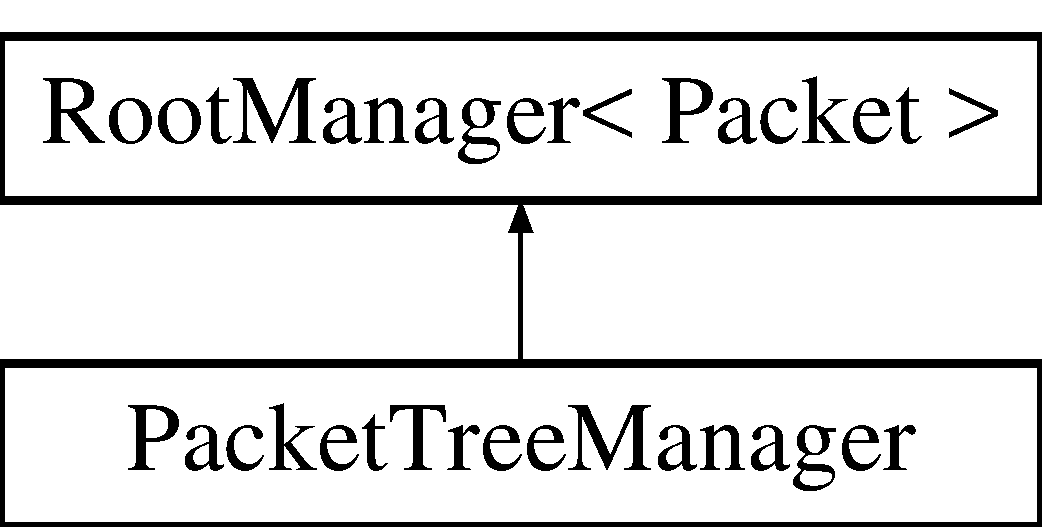
\includegraphics[height=2.000000cm]{class_packet_tree_manager}
\end{center}
\end{figure}
\subsection*{Public Member Functions}
\begin{DoxyCompactItemize}
\item 
\hyperlink{class_packet_tree_manager_ab5393bcd3be4255232d9750cf85a4b13}{Packet\+Tree\+Manager} (std\+::shared\+\_\+ptr$<$ const \hyperlink{class_config}{Config} $>$ config, const std\+::string outfile\+Name)
\begin{DoxyCompactList}\small\item\em Constructor. \end{DoxyCompactList}\item 
void \hyperlink{class_packet_tree_manager_a855e71512fe6365c11f312584afff70a}{add} (std\+::unique\+\_\+ptr$<$ \hyperlink{class_packet}{Packet} $>$ packet) final
\begin{DoxyCompactList}\small\item\em Adds a packet to the tree, then destroys the packet. \end{DoxyCompactList}\end{DoxyCompactItemize}
\subsection*{Private Member Functions}
\begin{DoxyCompactItemize}
\item 
void \hyperlink{class_packet_tree_manager_a3e2aa24c5acd8a87b15cfff2d011f30b}{set\+Up\+Branches} ()
\begin{DoxyCompactList}\small\item\em Sets up the branches of the tree. \end{DoxyCompactList}\end{DoxyCompactItemize}
\subsection*{Private Attributes}
\begin{DoxyCompactItemize}
\item 
U\+Int\+\_\+t \hyperlink{class_packet_tree_manager_a5a07d44397bd25e8fc1e9db65f472d1a}{b\+\_\+tdc\+ID} = 0
\begin{DoxyCompactList}\small\item\em Branch Variable\+: T\+DC ID. \end{DoxyCompactList}\item 
U\+Int\+\_\+t \hyperlink{class_packet_tree_manager_a854d865fd2916a85e22560fee8a5c592}{b\+\_\+event\+ID} = 0
\begin{DoxyCompactList}\small\item\em Branch Variable\+: \hyperlink{class_event}{Event} ID. \end{DoxyCompactList}\item 
U\+Int\+\_\+t \hyperlink{class_packet_tree_manager_a3f7da74c8d3e4f3323c7ffdb8b845c45}{b\+\_\+bunch\+ID} = 0
\begin{DoxyCompactList}\small\item\em Branch Variable\+: Bunch ID. \end{DoxyCompactList}\item 
U\+Int\+\_\+t \hyperlink{class_packet_tree_manager_ad7d8e0343e3e5f949dc20e591b2e6b2b}{b\+\_\+word\+Count} = 0
\begin{DoxyCompactList}\small\item\em Branch Variable\+: Word Count. \end{DoxyCompactList}\item 
U\+Int\+\_\+t \hyperlink{class_packet_tree_manager_a710e3e4d48e842b512720774ab05e83a}{b\+\_\+roc\+Time} = 0
\begin{DoxyCompactList}\small\item\em Branch Variable\+: R\+OC time. \end{DoxyCompactList}\item 
U\+Int\+\_\+t \hyperlink{class_packet_tree_manager_a146354471ea64dae67959dd833c100c2}{b\+\_\+n\+Leading\+Edges} = 0
\begin{DoxyCompactList}\small\item\em Branch Variable\+: Number of leading edges. \end{DoxyCompactList}\item 
U\+Int\+\_\+t $\ast$ \hyperlink{class_packet_tree_manager_a14090e7e05b84788ac03b36843edb926}{b\+\_\+leading\+Channel\+ID} = nullptr
\begin{DoxyCompactList}\small\item\em Branch Variable \mbox{[}n\+Leading\+Edges\mbox{]}\+: Channel ID. \end{DoxyCompactList}\item 
U\+Int\+\_\+t $\ast$ \hyperlink{class_packet_tree_manager_aaba5588ce24ffbbfaa7602f31856a438}{b\+\_\+leading\+Timestamp} = nullptr
\begin{DoxyCompactList}\small\item\em Branch Variable \mbox{[}n\+Leading\+Edges\mbox{]}\+: Timestamp. \end{DoxyCompactList}\item 
U\+Int\+\_\+t $\ast$ \hyperlink{class_packet_tree_manager_ae28ebfaf5833b8c5fa4fc264a50302dd}{b\+\_\+leading\+T\+D\+C\+Bin} = nullptr
\begin{DoxyCompactList}\small\item\em Branch Variable \mbox{[}n\+Leading\+Edges\mbox{]}\+: Timestamp T\+DC Bin. \end{DoxyCompactList}\item 
U\+Int\+\_\+t \hyperlink{class_packet_tree_manager_a64f60068f8f3d5d2531a61d11b877b85}{b\+\_\+n\+Trailing\+Edges} = 0
\begin{DoxyCompactList}\small\item\em Branch Variable\+: Number of trailing edges. \end{DoxyCompactList}\item 
U\+Int\+\_\+t $\ast$ \hyperlink{class_packet_tree_manager_ad8e33ea8a6cde82babd0a8a89225b4ae}{b\+\_\+trailing\+Channel\+ID} = nullptr
\begin{DoxyCompactList}\small\item\em Branch Variable \mbox{[}n\+Trailing\+Edges\mbox{]}\+: Channel ID. \end{DoxyCompactList}\item 
U\+Int\+\_\+t $\ast$ \hyperlink{class_packet_tree_manager_ac850c2a253026809b1118a572ede792c}{b\+\_\+trailing\+Timestamp} = nullptr
\begin{DoxyCompactList}\small\item\em Branch Variable \mbox{[}n\+Trailing\+Edges\mbox{]}\+: Timestamp. \end{DoxyCompactList}\item 
U\+Int\+\_\+t $\ast$ \hyperlink{class_packet_tree_manager_a80a9821f7a5d2af88a8daf4569f60e17}{b\+\_\+trailing\+T\+D\+C\+Bin} = nullptr
\begin{DoxyCompactList}\small\item\em Branch Variable \mbox{[}n\+Trailing\+Edges\mbox{]}\+: Timestamp T\+DC Bin. \end{DoxyCompactList}\end{DoxyCompactItemize}
\subsection*{Static Private Attributes}
\begin{DoxyCompactItemize}
\item 
static constexpr unsigned int \hyperlink{class_packet_tree_manager_a4ba06517ad1cb912ff70df1ff69231a5}{s\+\_\+max\+Edges} = 100
\begin{DoxyCompactList}\small\item\em Array size for edge branches. \end{DoxyCompactList}\end{DoxyCompactItemize}
\subsection*{Additional Inherited Members}


\subsection{Detailed Description}
Class which manages storage of \hyperlink{class_packet}{Packet} data in root file output. 

\subsection{Constructor \& Destructor Documentation}
\mbox{\Hypertarget{class_packet_tree_manager_ab5393bcd3be4255232d9750cf85a4b13}\label{class_packet_tree_manager_ab5393bcd3be4255232d9750cf85a4b13}} 
\index{Packet\+Tree\+Manager@{Packet\+Tree\+Manager}!Packet\+Tree\+Manager@{Packet\+Tree\+Manager}}
\index{Packet\+Tree\+Manager@{Packet\+Tree\+Manager}!Packet\+Tree\+Manager@{Packet\+Tree\+Manager}}
\subsubsection{\texorpdfstring{Packet\+Tree\+Manager()}{PacketTreeManager()}}
{\footnotesize\ttfamily Packet\+Tree\+Manager\+::\+Packet\+Tree\+Manager (\begin{DoxyParamCaption}\item[{std\+::shared\+\_\+ptr$<$ const \hyperlink{class_config}{Config} $>$}]{config,  }\item[{const std\+::string}]{outfile\+Name }\end{DoxyParamCaption})}



Constructor. 


\begin{DoxyParams}{Parameters}
{\em config} & Ptr to program configuration \\
\hline
{\em outfile\+Name} & The desired output file name \\
\hline
\end{DoxyParams}


\subsection{Member Function Documentation}
\mbox{\Hypertarget{class_packet_tree_manager_a855e71512fe6365c11f312584afff70a}\label{class_packet_tree_manager_a855e71512fe6365c11f312584afff70a}} 
\index{Packet\+Tree\+Manager@{Packet\+Tree\+Manager}!add@{add}}
\index{add@{add}!Packet\+Tree\+Manager@{Packet\+Tree\+Manager}}
\subsubsection{\texorpdfstring{add()}{add()}}
{\footnotesize\ttfamily void Packet\+Tree\+Manager\+::add (\begin{DoxyParamCaption}\item[{std\+::unique\+\_\+ptr$<$ \hyperlink{class_packet}{Packet} $>$}]{packet }\end{DoxyParamCaption})\hspace{0.3cm}{\ttfamily [final]}, {\ttfamily [virtual]}}



Adds a packet to the tree, then destroys the packet. 

Overload of \hyperlink{class_root_manager}{Root\+Manager} add. 

Implements \hyperlink{class_root_manager_a2f05eb45d5eaee1f9f12e299395652fb}{Root\+Manager$<$ Packet $>$}.

\mbox{\Hypertarget{class_packet_tree_manager_a3e2aa24c5acd8a87b15cfff2d011f30b}\label{class_packet_tree_manager_a3e2aa24c5acd8a87b15cfff2d011f30b}} 
\index{Packet\+Tree\+Manager@{Packet\+Tree\+Manager}!set\+Up\+Branches@{set\+Up\+Branches}}
\index{set\+Up\+Branches@{set\+Up\+Branches}!Packet\+Tree\+Manager@{Packet\+Tree\+Manager}}
\subsubsection{\texorpdfstring{set\+Up\+Branches()}{setUpBranches()}}
{\footnotesize\ttfamily void Packet\+Tree\+Manager\+::set\+Up\+Branches (\begin{DoxyParamCaption}{ }\end{DoxyParamCaption})\hspace{0.3cm}{\ttfamily [private]}}



Sets up the branches of the tree. 



\subsection{Member Data Documentation}
\mbox{\Hypertarget{class_packet_tree_manager_a3f7da74c8d3e4f3323c7ffdb8b845c45}\label{class_packet_tree_manager_a3f7da74c8d3e4f3323c7ffdb8b845c45}} 
\index{Packet\+Tree\+Manager@{Packet\+Tree\+Manager}!b\+\_\+bunch\+ID@{b\+\_\+bunch\+ID}}
\index{b\+\_\+bunch\+ID@{b\+\_\+bunch\+ID}!Packet\+Tree\+Manager@{Packet\+Tree\+Manager}}
\subsubsection{\texorpdfstring{b\+\_\+bunch\+ID}{b\_bunchID}}
{\footnotesize\ttfamily U\+Int\+\_\+t Packet\+Tree\+Manager\+::b\+\_\+bunch\+ID = 0\hspace{0.3cm}{\ttfamily [private]}}



Branch Variable\+: Bunch ID. 

\mbox{\Hypertarget{class_packet_tree_manager_a854d865fd2916a85e22560fee8a5c592}\label{class_packet_tree_manager_a854d865fd2916a85e22560fee8a5c592}} 
\index{Packet\+Tree\+Manager@{Packet\+Tree\+Manager}!b\+\_\+event\+ID@{b\+\_\+event\+ID}}
\index{b\+\_\+event\+ID@{b\+\_\+event\+ID}!Packet\+Tree\+Manager@{Packet\+Tree\+Manager}}
\subsubsection{\texorpdfstring{b\+\_\+event\+ID}{b\_eventID}}
{\footnotesize\ttfamily U\+Int\+\_\+t Packet\+Tree\+Manager\+::b\+\_\+event\+ID = 0\hspace{0.3cm}{\ttfamily [private]}}



Branch Variable\+: \hyperlink{class_event}{Event} ID. 

\mbox{\Hypertarget{class_packet_tree_manager_a14090e7e05b84788ac03b36843edb926}\label{class_packet_tree_manager_a14090e7e05b84788ac03b36843edb926}} 
\index{Packet\+Tree\+Manager@{Packet\+Tree\+Manager}!b\+\_\+leading\+Channel\+ID@{b\+\_\+leading\+Channel\+ID}}
\index{b\+\_\+leading\+Channel\+ID@{b\+\_\+leading\+Channel\+ID}!Packet\+Tree\+Manager@{Packet\+Tree\+Manager}}
\subsubsection{\texorpdfstring{b\+\_\+leading\+Channel\+ID}{b\_leadingChannelID}}
{\footnotesize\ttfamily U\+Int\+\_\+t$\ast$ Packet\+Tree\+Manager\+::b\+\_\+leading\+Channel\+ID = nullptr\hspace{0.3cm}{\ttfamily [private]}}



Branch Variable \mbox{[}n\+Leading\+Edges\mbox{]}\+: Channel ID. 

\mbox{\Hypertarget{class_packet_tree_manager_ae28ebfaf5833b8c5fa4fc264a50302dd}\label{class_packet_tree_manager_ae28ebfaf5833b8c5fa4fc264a50302dd}} 
\index{Packet\+Tree\+Manager@{Packet\+Tree\+Manager}!b\+\_\+leading\+T\+D\+C\+Bin@{b\+\_\+leading\+T\+D\+C\+Bin}}
\index{b\+\_\+leading\+T\+D\+C\+Bin@{b\+\_\+leading\+T\+D\+C\+Bin}!Packet\+Tree\+Manager@{Packet\+Tree\+Manager}}
\subsubsection{\texorpdfstring{b\+\_\+leading\+T\+D\+C\+Bin}{b\_leadingTDCBin}}
{\footnotesize\ttfamily U\+Int\+\_\+t$\ast$ Packet\+Tree\+Manager\+::b\+\_\+leading\+T\+D\+C\+Bin = nullptr\hspace{0.3cm}{\ttfamily [private]}}



Branch Variable \mbox{[}n\+Leading\+Edges\mbox{]}\+: Timestamp T\+DC Bin. 

\mbox{\Hypertarget{class_packet_tree_manager_aaba5588ce24ffbbfaa7602f31856a438}\label{class_packet_tree_manager_aaba5588ce24ffbbfaa7602f31856a438}} 
\index{Packet\+Tree\+Manager@{Packet\+Tree\+Manager}!b\+\_\+leading\+Timestamp@{b\+\_\+leading\+Timestamp}}
\index{b\+\_\+leading\+Timestamp@{b\+\_\+leading\+Timestamp}!Packet\+Tree\+Manager@{Packet\+Tree\+Manager}}
\subsubsection{\texorpdfstring{b\+\_\+leading\+Timestamp}{b\_leadingTimestamp}}
{\footnotesize\ttfamily U\+Int\+\_\+t$\ast$ Packet\+Tree\+Manager\+::b\+\_\+leading\+Timestamp = nullptr\hspace{0.3cm}{\ttfamily [private]}}



Branch Variable \mbox{[}n\+Leading\+Edges\mbox{]}\+: Timestamp. 

\mbox{\Hypertarget{class_packet_tree_manager_a146354471ea64dae67959dd833c100c2}\label{class_packet_tree_manager_a146354471ea64dae67959dd833c100c2}} 
\index{Packet\+Tree\+Manager@{Packet\+Tree\+Manager}!b\+\_\+n\+Leading\+Edges@{b\+\_\+n\+Leading\+Edges}}
\index{b\+\_\+n\+Leading\+Edges@{b\+\_\+n\+Leading\+Edges}!Packet\+Tree\+Manager@{Packet\+Tree\+Manager}}
\subsubsection{\texorpdfstring{b\+\_\+n\+Leading\+Edges}{b\_nLeadingEdges}}
{\footnotesize\ttfamily U\+Int\+\_\+t Packet\+Tree\+Manager\+::b\+\_\+n\+Leading\+Edges = 0\hspace{0.3cm}{\ttfamily [private]}}



Branch Variable\+: Number of leading edges. 

\mbox{\Hypertarget{class_packet_tree_manager_a64f60068f8f3d5d2531a61d11b877b85}\label{class_packet_tree_manager_a64f60068f8f3d5d2531a61d11b877b85}} 
\index{Packet\+Tree\+Manager@{Packet\+Tree\+Manager}!b\+\_\+n\+Trailing\+Edges@{b\+\_\+n\+Trailing\+Edges}}
\index{b\+\_\+n\+Trailing\+Edges@{b\+\_\+n\+Trailing\+Edges}!Packet\+Tree\+Manager@{Packet\+Tree\+Manager}}
\subsubsection{\texorpdfstring{b\+\_\+n\+Trailing\+Edges}{b\_nTrailingEdges}}
{\footnotesize\ttfamily U\+Int\+\_\+t Packet\+Tree\+Manager\+::b\+\_\+n\+Trailing\+Edges = 0\hspace{0.3cm}{\ttfamily [private]}}



Branch Variable\+: Number of trailing edges. 

\mbox{\Hypertarget{class_packet_tree_manager_a710e3e4d48e842b512720774ab05e83a}\label{class_packet_tree_manager_a710e3e4d48e842b512720774ab05e83a}} 
\index{Packet\+Tree\+Manager@{Packet\+Tree\+Manager}!b\+\_\+roc\+Time@{b\+\_\+roc\+Time}}
\index{b\+\_\+roc\+Time@{b\+\_\+roc\+Time}!Packet\+Tree\+Manager@{Packet\+Tree\+Manager}}
\subsubsection{\texorpdfstring{b\+\_\+roc\+Time}{b\_rocTime}}
{\footnotesize\ttfamily U\+Int\+\_\+t Packet\+Tree\+Manager\+::b\+\_\+roc\+Time = 0\hspace{0.3cm}{\ttfamily [private]}}



Branch Variable\+: R\+OC time. 

\mbox{\Hypertarget{class_packet_tree_manager_a5a07d44397bd25e8fc1e9db65f472d1a}\label{class_packet_tree_manager_a5a07d44397bd25e8fc1e9db65f472d1a}} 
\index{Packet\+Tree\+Manager@{Packet\+Tree\+Manager}!b\+\_\+tdc\+ID@{b\+\_\+tdc\+ID}}
\index{b\+\_\+tdc\+ID@{b\+\_\+tdc\+ID}!Packet\+Tree\+Manager@{Packet\+Tree\+Manager}}
\subsubsection{\texorpdfstring{b\+\_\+tdc\+ID}{b\_tdcID}}
{\footnotesize\ttfamily U\+Int\+\_\+t Packet\+Tree\+Manager\+::b\+\_\+tdc\+ID = 0\hspace{0.3cm}{\ttfamily [private]}}



Branch Variable\+: T\+DC ID. 

\mbox{\Hypertarget{class_packet_tree_manager_ad8e33ea8a6cde82babd0a8a89225b4ae}\label{class_packet_tree_manager_ad8e33ea8a6cde82babd0a8a89225b4ae}} 
\index{Packet\+Tree\+Manager@{Packet\+Tree\+Manager}!b\+\_\+trailing\+Channel\+ID@{b\+\_\+trailing\+Channel\+ID}}
\index{b\+\_\+trailing\+Channel\+ID@{b\+\_\+trailing\+Channel\+ID}!Packet\+Tree\+Manager@{Packet\+Tree\+Manager}}
\subsubsection{\texorpdfstring{b\+\_\+trailing\+Channel\+ID}{b\_trailingChannelID}}
{\footnotesize\ttfamily U\+Int\+\_\+t$\ast$ Packet\+Tree\+Manager\+::b\+\_\+trailing\+Channel\+ID = nullptr\hspace{0.3cm}{\ttfamily [private]}}



Branch Variable \mbox{[}n\+Trailing\+Edges\mbox{]}\+: Channel ID. 

\mbox{\Hypertarget{class_packet_tree_manager_a80a9821f7a5d2af88a8daf4569f60e17}\label{class_packet_tree_manager_a80a9821f7a5d2af88a8daf4569f60e17}} 
\index{Packet\+Tree\+Manager@{Packet\+Tree\+Manager}!b\+\_\+trailing\+T\+D\+C\+Bin@{b\+\_\+trailing\+T\+D\+C\+Bin}}
\index{b\+\_\+trailing\+T\+D\+C\+Bin@{b\+\_\+trailing\+T\+D\+C\+Bin}!Packet\+Tree\+Manager@{Packet\+Tree\+Manager}}
\subsubsection{\texorpdfstring{b\+\_\+trailing\+T\+D\+C\+Bin}{b\_trailingTDCBin}}
{\footnotesize\ttfamily U\+Int\+\_\+t$\ast$ Packet\+Tree\+Manager\+::b\+\_\+trailing\+T\+D\+C\+Bin = nullptr\hspace{0.3cm}{\ttfamily [private]}}



Branch Variable \mbox{[}n\+Trailing\+Edges\mbox{]}\+: Timestamp T\+DC Bin. 

\mbox{\Hypertarget{class_packet_tree_manager_ac850c2a253026809b1118a572ede792c}\label{class_packet_tree_manager_ac850c2a253026809b1118a572ede792c}} 
\index{Packet\+Tree\+Manager@{Packet\+Tree\+Manager}!b\+\_\+trailing\+Timestamp@{b\+\_\+trailing\+Timestamp}}
\index{b\+\_\+trailing\+Timestamp@{b\+\_\+trailing\+Timestamp}!Packet\+Tree\+Manager@{Packet\+Tree\+Manager}}
\subsubsection{\texorpdfstring{b\+\_\+trailing\+Timestamp}{b\_trailingTimestamp}}
{\footnotesize\ttfamily U\+Int\+\_\+t$\ast$ Packet\+Tree\+Manager\+::b\+\_\+trailing\+Timestamp = nullptr\hspace{0.3cm}{\ttfamily [private]}}



Branch Variable \mbox{[}n\+Trailing\+Edges\mbox{]}\+: Timestamp. 

\mbox{\Hypertarget{class_packet_tree_manager_ad7d8e0343e3e5f949dc20e591b2e6b2b}\label{class_packet_tree_manager_ad7d8e0343e3e5f949dc20e591b2e6b2b}} 
\index{Packet\+Tree\+Manager@{Packet\+Tree\+Manager}!b\+\_\+word\+Count@{b\+\_\+word\+Count}}
\index{b\+\_\+word\+Count@{b\+\_\+word\+Count}!Packet\+Tree\+Manager@{Packet\+Tree\+Manager}}
\subsubsection{\texorpdfstring{b\+\_\+word\+Count}{b\_wordCount}}
{\footnotesize\ttfamily U\+Int\+\_\+t Packet\+Tree\+Manager\+::b\+\_\+word\+Count = 0\hspace{0.3cm}{\ttfamily [private]}}



Branch Variable\+: Word Count. 

\mbox{\Hypertarget{class_packet_tree_manager_a4ba06517ad1cb912ff70df1ff69231a5}\label{class_packet_tree_manager_a4ba06517ad1cb912ff70df1ff69231a5}} 
\index{Packet\+Tree\+Manager@{Packet\+Tree\+Manager}!s\+\_\+max\+Edges@{s\+\_\+max\+Edges}}
\index{s\+\_\+max\+Edges@{s\+\_\+max\+Edges}!Packet\+Tree\+Manager@{Packet\+Tree\+Manager}}
\subsubsection{\texorpdfstring{s\+\_\+max\+Edges}{s\_maxEdges}}
{\footnotesize\ttfamily constexpr unsigned int Packet\+Tree\+Manager\+::s\+\_\+max\+Edges = 100\hspace{0.3cm}{\ttfamily [static]}, {\ttfamily [private]}}



Array size for edge branches. 



The documentation for this class was generated from the following files\+:\begin{DoxyCompactItemize}
\item 
Root/inc/\hyperlink{_packet_tree_manager_8hpp}{Packet\+Tree\+Manager.\+hpp}\item 
Root/src/\hyperlink{_packet_tree_manager_8cpp}{Packet\+Tree\+Manager.\+cpp}\end{DoxyCompactItemize}

\hypertarget{class_processor}{}\section{Processor Class Reference}
\label{class_processor}\index{Processor@{Processor}}


Class which manages overall processing of data.  




{\ttfamily \#include $<$Processor.\+hpp$>$}

\subsection*{Public Member Functions}
\begin{DoxyCompactItemize}
\item 
\hyperlink{class_processor_a1cc4421ebb02f40665336598c1334c55}{Processor} (std\+::unique\+\_\+ptr$<$ const \hyperlink{class_config}{Config} $>$ config)
\item 
void \hyperlink{class_processor_a4186d391ddee1f68d763931dad346c4a}{process\+Files} (const std\+::vector$<$ std\+::string $>$ file\+Names)
\end{DoxyCompactItemize}
\subsection*{Private Types}
\begin{DoxyCompactItemize}
\item 
using \hyperlink{class_processor_a0cfd8ed0721769db91c142a19a392e0f}{packet\+Buffer} = \hyperlink{class_thread_safe_queue}{Thread\+Safe\+Queue}$<$ std\+::unique\+\_\+ptr$<$ \hyperlink{class_packet}{Packet} $>$ $>$
\end{DoxyCompactItemize}
\subsection*{Private Member Functions}
\begin{DoxyCompactItemize}
\item 
void \hyperlink{class_processor_aa9ad1e9d6f3d217e23649e42cd07de90}{initialize\+Packet\+Buffers} (const std\+::list$<$ unsigned int $>$ \&tdc\+I\+Ds)
\begin{DoxyCompactList}\small\item\em Initilises a packet buffer for each T\+DC ID. \end{DoxyCompactList}\item 
void \hyperlink{class_processor_a8dc09976d642ca778f5aa606b526a510}{process\+File} (const std\+::string file\+Name)
\begin{DoxyCompactList}\small\item\em Make Word Bundles (has R\+OC value and words found preceding it) \end{DoxyCompactList}\item 
void \hyperlink{class_processor_a31c772cd0725c185b53d271b6149c400}{read\+Header\+Line} (std\+::ifstream \&input\+Data, unsigned int \&readout\+Board\+Number, unsigned int \&n\+Data\+Bytes)
\begin{DoxyCompactList}\small\item\em Reads Header Line, storing information in readout\+Board\+Number and n\+Data\+Bytes. \end{DoxyCompactList}\item 
std\+::array$<$ unsigned int, 4 $>$ \hyperlink{class_processor_ad64350d14782bb238703023cb56613ef}{read\+Data\+Block} (std\+::ifstream \&input\+Data)
\begin{DoxyCompactList}\small\item\em Reads a data block, returning the words in a std\+::array object. \end{DoxyCompactList}\item 
void \hyperlink{class_processor_a395245680ed38f6c7bf568f5af262860}{make\+Packets} ()
\begin{DoxyCompactList}\small\item\em Process word bundles into packets. \end{DoxyCompactList}\item 
void \hyperlink{class_processor_ae06672fc3ac6ef73525b64d4f9f769e7}{make\+Events} ()
\begin{DoxyCompactList}\small\item\em Build Events from Packets. \end{DoxyCompactList}\end{DoxyCompactItemize}
\subsection*{Private Attributes}
\begin{DoxyCompactItemize}
\item 
const \hyperlink{_modes_enum_8hpp_a3dfe11cf1a3a8121f6cd7fec4bf5947e}{Run\+Mode} \hyperlink{class_processor_ac22f412163181f546d847ce23d71978d}{m\+\_\+mode} = \hyperlink{_modes_enum_8hpp_a3dfe11cf1a3a8121f6cd7fec4bf5947ea8cf5e1a2a32430916501be0579e5303b}{Run\+Mode\+::\+Low\+Level}
\begin{DoxyCompactList}\small\item\em Write Events to R\+O\+OT file. \end{DoxyCompactList}\item 
const std\+::list$<$ unsigned int $>$ \hyperlink{class_processor_a8eaa993665bf2a2ed71f84ffc0630574}{m\+\_\+tdc\+I\+Ds} \{ 8, 9, 10, 11, 12, 13, 14, 15 \}
\begin{DoxyCompactList}\small\item\em List of T\+DC I\+Ds (needs to be set by config) \end{DoxyCompactList}\item 
const std\+::set$<$ unsigned int $>$ \hyperlink{class_processor_a78d13a8646a95290e0b74bdd40c75639}{filler\+Words} = \{ 0x\+A0\+A0\+A0\+A0, 0x\+B0\+B0\+B0\+B0, 0x\+C0\+C0\+C0\+C0, 0x\+D0\+D0\+D0\+D0 \}
\begin{DoxyCompactList}\small\item\em Set containing filler words (move to config?) \end{DoxyCompactList}\item 
std\+::unique\+\_\+ptr$<$ const \hyperlink{class_config}{Config} $>$ \hyperlink{class_processor_aa1ac0a603b269d9f0e1a90ec318c1525}{m\+\_\+config}
\begin{DoxyCompactList}\small\item\em Pointer to configuration object. \end{DoxyCompactList}\item 
\hyperlink{class_thread_safe_queue}{Thread\+Safe\+Queue}$<$ std\+::unique\+\_\+ptr$<$ \hyperlink{class_word_bundle}{Word\+Bundle} $>$ $>$ \hyperlink{class_processor_a1ec54aa38a8c50dc77877e17feed6142}{m\+\_\+word\+Bundle\+Buffer}
\begin{DoxyCompactList}\small\item\em \hyperlink{class_word_bundle}{Word\+Bundle} Buffers. \end{DoxyCompactList}\item 
std\+::unordered\+\_\+map$<$ unsigned int, \hyperlink{class_processor_a0cfd8ed0721769db91c142a19a392e0f}{packet\+Buffer} $>$ \hyperlink{class_processor_ab75c789ec03e38e8621f000332daa285}{m\+\_\+packet\+Buffers}
\begin{DoxyCompactList}\small\item\em \hyperlink{class_packet}{Packet} Buffers. \end{DoxyCompactList}\item 
\hyperlink{class_thread_safe_event_map}{Thread\+Safe\+Event\+Map} \hyperlink{class_processor_a7cb15fbab19fceb6bc5a607629ff5040}{m\+\_\+event\+Buffer}
\begin{DoxyCompactList}\small\item\em \hyperlink{class_event}{Event} Buffer. \end{DoxyCompactList}\end{DoxyCompactItemize}


\subsection{Detailed Description}
Class which manages overall processing of data. 

Is setup based on values stores in \hyperlink{class_config}{Config} 

\subsection{Member Typedef Documentation}
\mbox{\Hypertarget{class_processor_a0cfd8ed0721769db91c142a19a392e0f}\label{class_processor_a0cfd8ed0721769db91c142a19a392e0f}} 
\index{Processor@{Processor}!packet\+Buffer@{packet\+Buffer}}
\index{packet\+Buffer@{packet\+Buffer}!Processor@{Processor}}
\subsubsection{\texorpdfstring{packet\+Buffer}{packetBuffer}}
{\footnotesize\ttfamily using \hyperlink{class_processor_a0cfd8ed0721769db91c142a19a392e0f}{Processor\+::packet\+Buffer} =  \hyperlink{class_thread_safe_queue}{Thread\+Safe\+Queue}$<$ std\+::unique\+\_\+ptr$<$\hyperlink{class_packet}{Packet}$>$ $>$\hspace{0.3cm}{\ttfamily [private]}}



\subsection{Constructor \& Destructor Documentation}
\mbox{\Hypertarget{class_processor_a1cc4421ebb02f40665336598c1334c55}\label{class_processor_a1cc4421ebb02f40665336598c1334c55}} 
\index{Processor@{Processor}!Processor@{Processor}}
\index{Processor@{Processor}!Processor@{Processor}}
\subsubsection{\texorpdfstring{Processor()}{Processor()}}
{\footnotesize\ttfamily Processor\+::\+Processor (\begin{DoxyParamCaption}\item[{std\+::unique\+\_\+ptr$<$ const \hyperlink{class_config}{Config} $>$}]{config }\end{DoxyParamCaption})}



\subsection{Member Function Documentation}
\mbox{\Hypertarget{class_processor_aa9ad1e9d6f3d217e23649e42cd07de90}\label{class_processor_aa9ad1e9d6f3d217e23649e42cd07de90}} 
\index{Processor@{Processor}!initialize\+Packet\+Buffers@{initialize\+Packet\+Buffers}}
\index{initialize\+Packet\+Buffers@{initialize\+Packet\+Buffers}!Processor@{Processor}}
\subsubsection{\texorpdfstring{initialize\+Packet\+Buffers()}{initializePacketBuffers()}}
{\footnotesize\ttfamily void Processor\+::initialize\+Packet\+Buffers (\begin{DoxyParamCaption}\item[{const std\+::list$<$ unsigned int $>$ \&}]{tdc\+I\+Ds }\end{DoxyParamCaption})\hspace{0.3cm}{\ttfamily [private]}}



Initilises a packet buffer for each T\+DC ID. 

\mbox{\Hypertarget{class_processor_ae06672fc3ac6ef73525b64d4f9f769e7}\label{class_processor_ae06672fc3ac6ef73525b64d4f9f769e7}} 
\index{Processor@{Processor}!make\+Events@{make\+Events}}
\index{make\+Events@{make\+Events}!Processor@{Processor}}
\subsubsection{\texorpdfstring{make\+Events()}{makeEvents()}}
{\footnotesize\ttfamily void Processor\+::make\+Events (\begin{DoxyParamCaption}{ }\end{DoxyParamCaption})\hspace{0.3cm}{\ttfamily [private]}}



Build Events from Packets. 

\mbox{\Hypertarget{class_processor_a395245680ed38f6c7bf568f5af262860}\label{class_processor_a395245680ed38f6c7bf568f5af262860}} 
\index{Processor@{Processor}!make\+Packets@{make\+Packets}}
\index{make\+Packets@{make\+Packets}!Processor@{Processor}}
\subsubsection{\texorpdfstring{make\+Packets()}{makePackets()}}
{\footnotesize\ttfamily void Processor\+::make\+Packets (\begin{DoxyParamCaption}{ }\end{DoxyParamCaption})\hspace{0.3cm}{\ttfamily [private]}}



Process word bundles into packets. 

\mbox{\Hypertarget{class_processor_a8dc09976d642ca778f5aa606b526a510}\label{class_processor_a8dc09976d642ca778f5aa606b526a510}} 
\index{Processor@{Processor}!process\+File@{process\+File}}
\index{process\+File@{process\+File}!Processor@{Processor}}
\subsubsection{\texorpdfstring{process\+File()}{processFile()}}
{\footnotesize\ttfamily void Processor\+::process\+File (\begin{DoxyParamCaption}\item[{const std\+::string}]{file\+Name }\end{DoxyParamCaption})\hspace{0.3cm}{\ttfamily [private]}}



Make Word Bundles (has R\+OC value and words found preceding it) 

\mbox{\Hypertarget{class_processor_a4186d391ddee1f68d763931dad346c4a}\label{class_processor_a4186d391ddee1f68d763931dad346c4a}} 
\index{Processor@{Processor}!process\+Files@{process\+Files}}
\index{process\+Files@{process\+Files}!Processor@{Processor}}
\subsubsection{\texorpdfstring{process\+Files()}{processFiles()}}
{\footnotesize\ttfamily void Processor\+::process\+Files (\begin{DoxyParamCaption}\item[{const std\+::vector$<$ std\+::string $>$}]{file\+Names }\end{DoxyParamCaption})}

\mbox{\Hypertarget{class_processor_ad64350d14782bb238703023cb56613ef}\label{class_processor_ad64350d14782bb238703023cb56613ef}} 
\index{Processor@{Processor}!read\+Data\+Block@{read\+Data\+Block}}
\index{read\+Data\+Block@{read\+Data\+Block}!Processor@{Processor}}
\subsubsection{\texorpdfstring{read\+Data\+Block()}{readDataBlock()}}
{\footnotesize\ttfamily std\+::array$<$ unsigned int, 4 $>$ Processor\+::read\+Data\+Block (\begin{DoxyParamCaption}\item[{std\+::ifstream \&}]{input\+Data }\end{DoxyParamCaption})\hspace{0.3cm}{\ttfamily [private]}}



Reads a data block, returning the words in a std\+::array object. 

\mbox{\Hypertarget{class_processor_a31c772cd0725c185b53d271b6149c400}\label{class_processor_a31c772cd0725c185b53d271b6149c400}} 
\index{Processor@{Processor}!read\+Header\+Line@{read\+Header\+Line}}
\index{read\+Header\+Line@{read\+Header\+Line}!Processor@{Processor}}
\subsubsection{\texorpdfstring{read\+Header\+Line()}{readHeaderLine()}}
{\footnotesize\ttfamily void Processor\+::read\+Header\+Line (\begin{DoxyParamCaption}\item[{std\+::ifstream \&}]{input\+Data,  }\item[{unsigned int \&}]{readout\+Board\+Number,  }\item[{unsigned int \&}]{n\+Data\+Bytes }\end{DoxyParamCaption})\hspace{0.3cm}{\ttfamily [private]}}



Reads Header Line, storing information in readout\+Board\+Number and n\+Data\+Bytes. 



\subsection{Member Data Documentation}
\mbox{\Hypertarget{class_processor_a78d13a8646a95290e0b74bdd40c75639}\label{class_processor_a78d13a8646a95290e0b74bdd40c75639}} 
\index{Processor@{Processor}!filler\+Words@{filler\+Words}}
\index{filler\+Words@{filler\+Words}!Processor@{Processor}}
\subsubsection{\texorpdfstring{filler\+Words}{fillerWords}}
{\footnotesize\ttfamily const std\+::set$<$unsigned int$>$ Processor\+::filler\+Words = \{ 0x\+A0\+A0\+A0\+A0, 0x\+B0\+B0\+B0\+B0, 0x\+C0\+C0\+C0\+C0, 0x\+D0\+D0\+D0\+D0 \}\hspace{0.3cm}{\ttfamily [private]}}



Set containing filler words (move to config?) 

\mbox{\Hypertarget{class_processor_aa1ac0a603b269d9f0e1a90ec318c1525}\label{class_processor_aa1ac0a603b269d9f0e1a90ec318c1525}} 
\index{Processor@{Processor}!m\+\_\+config@{m\+\_\+config}}
\index{m\+\_\+config@{m\+\_\+config}!Processor@{Processor}}
\subsubsection{\texorpdfstring{m\+\_\+config}{m\_config}}
{\footnotesize\ttfamily std\+::unique\+\_\+ptr$<$const \hyperlink{class_config}{Config}$>$ Processor\+::m\+\_\+config\hspace{0.3cm}{\ttfamily [private]}}



Pointer to configuration object. 

\mbox{\Hypertarget{class_processor_a7cb15fbab19fceb6bc5a607629ff5040}\label{class_processor_a7cb15fbab19fceb6bc5a607629ff5040}} 
\index{Processor@{Processor}!m\+\_\+event\+Buffer@{m\+\_\+event\+Buffer}}
\index{m\+\_\+event\+Buffer@{m\+\_\+event\+Buffer}!Processor@{Processor}}
\subsubsection{\texorpdfstring{m\+\_\+event\+Buffer}{m\_eventBuffer}}
{\footnotesize\ttfamily \hyperlink{class_thread_safe_event_map}{Thread\+Safe\+Event\+Map} Processor\+::m\+\_\+event\+Buffer\hspace{0.3cm}{\ttfamily [private]}}



\hyperlink{class_event}{Event} Buffer. 

\mbox{\Hypertarget{class_processor_ac22f412163181f546d847ce23d71978d}\label{class_processor_ac22f412163181f546d847ce23d71978d}} 
\index{Processor@{Processor}!m\+\_\+mode@{m\+\_\+mode}}
\index{m\+\_\+mode@{m\+\_\+mode}!Processor@{Processor}}
\subsubsection{\texorpdfstring{m\+\_\+mode}{m\_mode}}
{\footnotesize\ttfamily const \hyperlink{_modes_enum_8hpp_a3dfe11cf1a3a8121f6cd7fec4bf5947e}{Run\+Mode} Processor\+::m\+\_\+mode = \hyperlink{_modes_enum_8hpp_a3dfe11cf1a3a8121f6cd7fec4bf5947ea8cf5e1a2a32430916501be0579e5303b}{Run\+Mode\+::\+Low\+Level}\hspace{0.3cm}{\ttfamily [private]}}



Write Events to R\+O\+OT file. 

\mbox{\Hypertarget{class_processor_ab75c789ec03e38e8621f000332daa285}\label{class_processor_ab75c789ec03e38e8621f000332daa285}} 
\index{Processor@{Processor}!m\+\_\+packet\+Buffers@{m\+\_\+packet\+Buffers}}
\index{m\+\_\+packet\+Buffers@{m\+\_\+packet\+Buffers}!Processor@{Processor}}
\subsubsection{\texorpdfstring{m\+\_\+packet\+Buffers}{m\_packetBuffers}}
{\footnotesize\ttfamily std\+::unordered\+\_\+map$<$ unsigned int, \hyperlink{class_processor_a0cfd8ed0721769db91c142a19a392e0f}{packet\+Buffer}$>$ Processor\+::m\+\_\+packet\+Buffers\hspace{0.3cm}{\ttfamily [private]}}



\hyperlink{class_packet}{Packet} Buffers. 

\mbox{\Hypertarget{class_processor_a8eaa993665bf2a2ed71f84ffc0630574}\label{class_processor_a8eaa993665bf2a2ed71f84ffc0630574}} 
\index{Processor@{Processor}!m\+\_\+tdc\+I\+Ds@{m\+\_\+tdc\+I\+Ds}}
\index{m\+\_\+tdc\+I\+Ds@{m\+\_\+tdc\+I\+Ds}!Processor@{Processor}}
\subsubsection{\texorpdfstring{m\+\_\+tdc\+I\+Ds}{m\_tdcIDs}}
{\footnotesize\ttfamily const std\+::list$<$unsigned int$>$ Processor\+::m\+\_\+tdc\+I\+Ds \{ 8, 9, 10, 11, 12, 13, 14, 15 \}\hspace{0.3cm}{\ttfamily [private]}}



List of T\+DC I\+Ds (needs to be set by config) 

\mbox{\Hypertarget{class_processor_a1ec54aa38a8c50dc77877e17feed6142}\label{class_processor_a1ec54aa38a8c50dc77877e17feed6142}} 
\index{Processor@{Processor}!m\+\_\+word\+Bundle\+Buffer@{m\+\_\+word\+Bundle\+Buffer}}
\index{m\+\_\+word\+Bundle\+Buffer@{m\+\_\+word\+Bundle\+Buffer}!Processor@{Processor}}
\subsubsection{\texorpdfstring{m\+\_\+word\+Bundle\+Buffer}{m\_wordBundleBuffer}}
{\footnotesize\ttfamily \hyperlink{class_thread_safe_queue}{Thread\+Safe\+Queue}$<$ std\+::unique\+\_\+ptr$<$\hyperlink{class_word_bundle}{Word\+Bundle}$>$ $>$ Processor\+::m\+\_\+word\+Bundle\+Buffer\hspace{0.3cm}{\ttfamily [private]}}



\hyperlink{class_word_bundle}{Word\+Bundle} Buffers. 



The documentation for this class was generated from the following files\+:\begin{DoxyCompactItemize}
\item 
Core/inc/\hyperlink{_processor_8hpp}{Processor.\+hpp}\item 
Core/src/\hyperlink{_processor_8cpp}{Processor.\+cpp}\end{DoxyCompactItemize}

\hypertarget{class_root_manager}{}\section{Root\+Manager$<$ T $>$ Class Template Reference}
\label{class_root_manager}\index{Root\+Manager$<$ T $>$@{Root\+Manager$<$ T $>$}}


Class which manages root output.  




{\ttfamily \#include $<$Root\+Manager.\+hpp$>$}

\subsection*{Public Member Functions}
\begin{DoxyCompactItemize}
\item 
\hyperlink{class_root_manager_a90ff78b3122c0b3fad62bc927778dda9}{Root\+Manager} (std\+::shared\+\_\+ptr$<$ const \hyperlink{class_config}{Config} $>$ config, const std\+::string out\+File\+Name, const std\+::string tree\+Name)
\begin{DoxyCompactList}\small\item\em Constructor. \end{DoxyCompactList}\item 
virtual \hyperlink{class_root_manager_a68a189a7705b9da1da82a95ef9840d61}{$\sim$\+Root\+Manager} ()
\begin{DoxyCompactList}\small\item\em Explicit deconstructor. \end{DoxyCompactList}\item 
virtual void \hyperlink{class_root_manager_a2f05eb45d5eaee1f9f12e299395652fb}{add} (std\+::unique\+\_\+ptr$<$ T $>$)=0
\begin{DoxyCompactList}\small\item\em Pure virtual method for adding information to the tree. \end{DoxyCompactList}\item 
void \hyperlink{class_root_manager_adbe916dd56e5ec51f89c7643c4847842}{write\+Tree} ()
\begin{DoxyCompactList}\small\item\em Writes the tree to the output file. \end{DoxyCompactList}\end{DoxyCompactItemize}
\subsection*{Protected Member Functions}
\begin{DoxyCompactItemize}
\item 
{\footnotesize template$<$class U $>$ }\\void \hyperlink{class_root_manager_aa1eaed1aa026059b8d00e729161c6a43}{setup\+Arr\+Branch} (const std\+::string branch\+Name, U $\ast$\&array\+Ptr, const std\+::string leaf\+Type, const unsigned int array\+Size)
\begin{DoxyCompactList}\small\item\em Helpful function to allocate memory for an array-\/style branch. \end{DoxyCompactList}\end{DoxyCompactItemize}
\subsection*{Protected Attributes}
\begin{DoxyCompactItemize}
\item 
std\+::mutex \hyperlink{class_root_manager_a8f8a185d6d25b3e1207416c7cd8c333c}{m\+\_\+mut}
\begin{DoxyCompactList}\small\item\em Mutex for thread safety. \end{DoxyCompactList}\item 
T\+Tree $\ast$ \hyperlink{class_root_manager_adfbcbba0248787d08a230508bb4136a6}{m\+\_\+tree} = nullptr
\begin{DoxyCompactList}\small\item\em Output T\+Tree. \end{DoxyCompactList}\end{DoxyCompactItemize}
\subsection*{Private Attributes}
\begin{DoxyCompactItemize}
\item 
T\+File $\ast$ \hyperlink{class_root_manager_a2f0257574f0eeac21c3628058a5d6ad9}{m\+\_\+out\+File} = nullptr
\begin{DoxyCompactList}\small\item\em Output file pointer. \end{DoxyCompactList}\item 
const T\+Named \hyperlink{class_root_manager_a14d81290e5a98ec6f62459f1016e7dcc}{m\+\_\+program\+Version}
\begin{DoxyCompactList}\small\item\em T\+Named which writes build version to output tree. \end{DoxyCompactList}\item 
const T\+Named \hyperlink{class_root_manager_a4d92834cf49004700cafa3afa3659cd5}{m\+\_\+channel\+Mapping}
\begin{DoxyCompactList}\small\item\em T\+Named to write channel mapping. \end{DoxyCompactList}\item 
const T\+Named \hyperlink{class_root_manager_a3f17186761c3e5b61e569bc3f3946ddb}{m\+\_\+edge\+Modifier}
\begin{DoxyCompactList}\small\item\em T\+Named to write edge modifier. \end{DoxyCompactList}\end{DoxyCompactItemize}


\subsection{Detailed Description}
\subsubsection*{template$<$class T$>$\newline
class Root\+Manager$<$ T $>$}

Class which manages root output. 


\begin{DoxyTemplParams}{Template Parameters}
{\em T} & The class which will be used to provide information for the root tree \\
\hline
\end{DoxyTemplParams}


\subsection{Constructor \& Destructor Documentation}
\mbox{\Hypertarget{class_root_manager_a90ff78b3122c0b3fad62bc927778dda9}\label{class_root_manager_a90ff78b3122c0b3fad62bc927778dda9}} 
\index{Root\+Manager@{Root\+Manager}!Root\+Manager@{Root\+Manager}}
\index{Root\+Manager@{Root\+Manager}!Root\+Manager@{Root\+Manager}}
\subsubsection{\texorpdfstring{Root\+Manager()}{RootManager()}}
{\footnotesize\ttfamily template$<$class T $>$ \\
\hyperlink{class_root_manager}{Root\+Manager}$<$ T $>$\+::\hyperlink{class_root_manager}{Root\+Manager} (\begin{DoxyParamCaption}\item[{std\+::shared\+\_\+ptr$<$ const \hyperlink{class_config}{Config} $>$}]{config,  }\item[{const std\+::string}]{out\+File\+Name,  }\item[{const std\+::string}]{tree\+Name }\end{DoxyParamCaption})}



Constructor. 


\begin{DoxyParams}{Parameters}
{\em config} & Ptr to program configuration \\
\hline
{\em out\+File\+Name} & The output root files name \\
\hline
{\em tree\+Name} & The desired ttree name \\
\hline
\end{DoxyParams}
\mbox{\Hypertarget{class_root_manager_a68a189a7705b9da1da82a95ef9840d61}\label{class_root_manager_a68a189a7705b9da1da82a95ef9840d61}} 
\index{Root\+Manager@{Root\+Manager}!````~Root\+Manager@{$\sim$\+Root\+Manager}}
\index{````~Root\+Manager@{$\sim$\+Root\+Manager}!Root\+Manager@{Root\+Manager}}
\subsubsection{\texorpdfstring{$\sim$\+Root\+Manager()}{~RootManager()}}
{\footnotesize\ttfamily template$<$class T $>$ \\
\hyperlink{class_root_manager}{Root\+Manager}$<$ T $>$\+::$\sim$\hyperlink{class_root_manager}{Root\+Manager} (\begin{DoxyParamCaption}{ }\end{DoxyParamCaption})\hspace{0.3cm}{\ttfamily [virtual]}}



Explicit deconstructor. 

Closes output file on deconstruction. Implicitly deletes move and copy constructors. 

\subsection{Member Function Documentation}
\mbox{\Hypertarget{class_root_manager_a2f05eb45d5eaee1f9f12e299395652fb}\label{class_root_manager_a2f05eb45d5eaee1f9f12e299395652fb}} 
\index{Root\+Manager@{Root\+Manager}!add@{add}}
\index{add@{add}!Root\+Manager@{Root\+Manager}}
\subsubsection{\texorpdfstring{add()}{add()}}
{\footnotesize\ttfamily template$<$class T$>$ \\
virtual void \hyperlink{class_root_manager}{Root\+Manager}$<$ T $>$\+::add (\begin{DoxyParamCaption}\item[{std\+::unique\+\_\+ptr$<$ T $>$}]{ }\end{DoxyParamCaption})\hspace{0.3cm}{\ttfamily [pure virtual]}}



Pure virtual method for adding information to the tree. 



Implemented in \hyperlink{class_event_tree_manager_acabb2f6c8dd0e08375b4cf8bf2c148fd}{Event\+Tree\+Manager}, and \hyperlink{class_packet_tree_manager_a855e71512fe6365c11f312584afff70a}{Packet\+Tree\+Manager}.

\mbox{\Hypertarget{class_root_manager_aa1eaed1aa026059b8d00e729161c6a43}\label{class_root_manager_aa1eaed1aa026059b8d00e729161c6a43}} 
\index{Root\+Manager@{Root\+Manager}!setup\+Arr\+Branch@{setup\+Arr\+Branch}}
\index{setup\+Arr\+Branch@{setup\+Arr\+Branch}!Root\+Manager@{Root\+Manager}}
\subsubsection{\texorpdfstring{setup\+Arr\+Branch()}{setupArrBranch()}}
{\footnotesize\ttfamily template$<$class T $>$ \\
template$<$class U $>$ \\
void \hyperlink{class_root_manager}{Root\+Manager}$<$ T $>$\+::setup\+Arr\+Branch (\begin{DoxyParamCaption}\item[{const std\+::string}]{branch\+Name,  }\item[{U $\ast$\&}]{array\+Ptr,  }\item[{const std\+::string}]{leaf\+Type,  }\item[{const unsigned int}]{array\+Size }\end{DoxyParamCaption})\hspace{0.3cm}{\ttfamily [protected]}}



Helpful function to allocate memory for an array-\/style branch. 


\begin{DoxyTemplParams}{Template Parameters}
{\em U} & The data type of the branch \\
\hline
\end{DoxyTemplParams}

\begin{DoxyParams}{Parameters}
{\em branch\+Name} & Desired Branch Name \\
\hline
{\em array\+Ptr} & Reference to pointer to be set \\
\hline
{\em leaf\+Type} & Leaf type (e.\+g. \char`\"{}/\+I\char`\"{} ) \\
\hline
{\em array\+Size} & Size of array to be allocated \\
\hline
\end{DoxyParams}
\mbox{\Hypertarget{class_root_manager_adbe916dd56e5ec51f89c7643c4847842}\label{class_root_manager_adbe916dd56e5ec51f89c7643c4847842}} 
\index{Root\+Manager@{Root\+Manager}!write\+Tree@{write\+Tree}}
\index{write\+Tree@{write\+Tree}!Root\+Manager@{Root\+Manager}}
\subsubsection{\texorpdfstring{write\+Tree()}{writeTree()}}
{\footnotesize\ttfamily template$<$class T $>$ \\
void \hyperlink{class_root_manager}{Root\+Manager}$<$ T $>$\+::write\+Tree (\begin{DoxyParamCaption}{ }\end{DoxyParamCaption})\hspace{0.3cm}{\ttfamily [inline]}}



Writes the tree to the output file. 



\subsection{Member Data Documentation}
\mbox{\Hypertarget{class_root_manager_a4d92834cf49004700cafa3afa3659cd5}\label{class_root_manager_a4d92834cf49004700cafa3afa3659cd5}} 
\index{Root\+Manager@{Root\+Manager}!m\+\_\+channel\+Mapping@{m\+\_\+channel\+Mapping}}
\index{m\+\_\+channel\+Mapping@{m\+\_\+channel\+Mapping}!Root\+Manager@{Root\+Manager}}
\subsubsection{\texorpdfstring{m\+\_\+channel\+Mapping}{m\_channelMapping}}
{\footnotesize\ttfamily template$<$class T$>$ \\
const T\+Named \hyperlink{class_root_manager}{Root\+Manager}$<$ T $>$\+::m\+\_\+channel\+Mapping\hspace{0.3cm}{\ttfamily [private]}}



T\+Named to write channel mapping. 

\mbox{\Hypertarget{class_root_manager_a3f17186761c3e5b61e569bc3f3946ddb}\label{class_root_manager_a3f17186761c3e5b61e569bc3f3946ddb}} 
\index{Root\+Manager@{Root\+Manager}!m\+\_\+edge\+Modifier@{m\+\_\+edge\+Modifier}}
\index{m\+\_\+edge\+Modifier@{m\+\_\+edge\+Modifier}!Root\+Manager@{Root\+Manager}}
\subsubsection{\texorpdfstring{m\+\_\+edge\+Modifier}{m\_edgeModifier}}
{\footnotesize\ttfamily template$<$class T$>$ \\
const T\+Named \hyperlink{class_root_manager}{Root\+Manager}$<$ T $>$\+::m\+\_\+edge\+Modifier\hspace{0.3cm}{\ttfamily [private]}}



T\+Named to write edge modifier. 

\mbox{\Hypertarget{class_root_manager_a8f8a185d6d25b3e1207416c7cd8c333c}\label{class_root_manager_a8f8a185d6d25b3e1207416c7cd8c333c}} 
\index{Root\+Manager@{Root\+Manager}!m\+\_\+mut@{m\+\_\+mut}}
\index{m\+\_\+mut@{m\+\_\+mut}!Root\+Manager@{Root\+Manager}}
\subsubsection{\texorpdfstring{m\+\_\+mut}{m\_mut}}
{\footnotesize\ttfamily template$<$class T$>$ \\
std\+::mutex \hyperlink{class_root_manager}{Root\+Manager}$<$ T $>$\+::m\+\_\+mut\hspace{0.3cm}{\ttfamily [mutable]}, {\ttfamily [protected]}}



Mutex for thread safety. 

\mbox{\Hypertarget{class_root_manager_a2f0257574f0eeac21c3628058a5d6ad9}\label{class_root_manager_a2f0257574f0eeac21c3628058a5d6ad9}} 
\index{Root\+Manager@{Root\+Manager}!m\+\_\+out\+File@{m\+\_\+out\+File}}
\index{m\+\_\+out\+File@{m\+\_\+out\+File}!Root\+Manager@{Root\+Manager}}
\subsubsection{\texorpdfstring{m\+\_\+out\+File}{m\_outFile}}
{\footnotesize\ttfamily template$<$class T$>$ \\
T\+File$\ast$ \hyperlink{class_root_manager}{Root\+Manager}$<$ T $>$\+::m\+\_\+out\+File = nullptr\hspace{0.3cm}{\ttfamily [private]}}



Output file pointer. 

\mbox{\Hypertarget{class_root_manager_a14d81290e5a98ec6f62459f1016e7dcc}\label{class_root_manager_a14d81290e5a98ec6f62459f1016e7dcc}} 
\index{Root\+Manager@{Root\+Manager}!m\+\_\+program\+Version@{m\+\_\+program\+Version}}
\index{m\+\_\+program\+Version@{m\+\_\+program\+Version}!Root\+Manager@{Root\+Manager}}
\subsubsection{\texorpdfstring{m\+\_\+program\+Version}{m\_programVersion}}
{\footnotesize\ttfamily template$<$class T$>$ \\
const T\+Named \hyperlink{class_root_manager}{Root\+Manager}$<$ T $>$\+::m\+\_\+program\+Version\hspace{0.3cm}{\ttfamily [private]}}



T\+Named which writes build version to output tree. 

\mbox{\Hypertarget{class_root_manager_adfbcbba0248787d08a230508bb4136a6}\label{class_root_manager_adfbcbba0248787d08a230508bb4136a6}} 
\index{Root\+Manager@{Root\+Manager}!m\+\_\+tree@{m\+\_\+tree}}
\index{m\+\_\+tree@{m\+\_\+tree}!Root\+Manager@{Root\+Manager}}
\subsubsection{\texorpdfstring{m\+\_\+tree}{m\_tree}}
{\footnotesize\ttfamily template$<$class T$>$ \\
T\+Tree$\ast$ \hyperlink{class_root_manager}{Root\+Manager}$<$ T $>$\+::m\+\_\+tree = nullptr\hspace{0.3cm}{\ttfamily [protected]}}



Output T\+Tree. 



The documentation for this class was generated from the following files\+:\begin{DoxyCompactItemize}
\item 
Root/inc/\hyperlink{_root_manager_8hpp}{Root\+Manager.\+hpp}\item 
Root/inc/\hyperlink{_root_manager_8inl}{Root\+Manager.\+inl}\end{DoxyCompactItemize}

\hypertarget{class_thread_safe_event_map}{}\section{Thread\+Safe\+Event\+Map Class Reference}
\label{class_thread_safe_event_map}\index{Thread\+Safe\+Event\+Map@{Thread\+Safe\+Event\+Map}}


{\ttfamily \#include $<$Thread\+Safe\+Event\+Map.\+hpp$>$}

\subsection*{Public Member Functions}
\begin{DoxyCompactItemize}
\item 
\hyperlink{class_thread_safe_event_map_ace03ee2a6017dfee50a61c68626d2345}{Thread\+Safe\+Event\+Map} (const std\+::list$<$ unsigned int $>$ tdc\+I\+Ds)
\begin{DoxyCompactList}\small\item\em Constructor. \end{DoxyCompactList}\item 
\hyperlink{class_thread_safe_event_map_a523d5bf6c632e3803e721ef3fd94e318}{Thread\+Safe\+Event\+Map} (const \hyperlink{class_thread_safe_event_map}{Thread\+Safe\+Event\+Map} \&other)=delete
\item 
\hyperlink{class_thread_safe_event_map}{Thread\+Safe\+Event\+Map} \& \hyperlink{class_thread_safe_event_map_a1d438208fcc3936dd4384a8a2b55bdf8}{operator=} (\hyperlink{class_thread_safe_event_map}{Thread\+Safe\+Event\+Map} other)=delete
\item 
\hyperlink{class_thread_safe_event_map_af28959f5fbd84f00d227d10e1b37e5e5}{Thread\+Safe\+Event\+Map} (const \hyperlink{class_thread_safe_event_map}{Thread\+Safe\+Event\+Map} \&\&other)=delete
\item 
\hyperlink{class_thread_safe_event_map}{Thread\+Safe\+Event\+Map} \& \hyperlink{class_thread_safe_event_map_a6bf7640fde19d7d6d4dedd5b06c09f84}{operator=} (\hyperlink{class_thread_safe_event_map}{Thread\+Safe\+Event\+Map} \&\&other)=delete
\item 
void \hyperlink{class_thread_safe_event_map_aafd485696f0a50da8afa864f04f0aa07}{add\+Packet} (std\+::unique\+\_\+ptr$<$ \hyperlink{class_packet}{Packet} $>$ packet)
\begin{DoxyCompactList}\small\item\em Add a packet to the events. \end{DoxyCompactList}\item 
bool \hyperlink{class_thread_safe_event_map_a9fb58083137d147811de5b93f991d044}{is\+Complete\+Stored} () const
\begin{DoxyCompactList}\small\item\em Is a complete event stored? \end{DoxyCompactList}\item 
bool \hyperlink{class_thread_safe_event_map_a203143086874b97171101871ba2c4f6f}{is\+Bloated} () const
\begin{DoxyCompactList}\small\item\em Returns whether the buffer is reaching capacity. \end{DoxyCompactList}\item 
std\+::vector$<$ std\+::unique\+\_\+ptr$<$ \hyperlink{class_event}{Event} $>$ $>$ \hyperlink{class_thread_safe_event_map_adc6c905693e3b9b54671299e7610d5b6}{pop\+To\+Complete} ()
\begin{DoxyCompactList}\small\item\em Returns events up to the next complete event. \end{DoxyCompactList}\item 
std\+::vector$<$ std\+::unique\+\_\+ptr$<$ \hyperlink{class_event}{Event} $>$ $>$ \hyperlink{class_thread_safe_event_map_a655bf86c67d1e8d0e8276b012f5fab8d}{dump\+Half} ()
\begin{DoxyCompactList}\small\item\em Returns first half of the events stored in the buffer. \end{DoxyCompactList}\item 
std\+::vector$<$ std\+::unique\+\_\+ptr$<$ \hyperlink{class_event}{Event} $>$ $>$ \hyperlink{class_thread_safe_event_map_af65f8dbd177f3db92d227b86839c275d}{dump\+All} ()
\begin{DoxyCompactList}\small\item\em Returns all events in the buffer. \end{DoxyCompactList}\end{DoxyCompactItemize}
\subsection*{Private Types}
\begin{DoxyCompactItemize}
\item 
using \hyperlink{class_thread_safe_event_map_a069c80cec7636a015d8a69574157d8d2}{event\+Map} = std\+::unordered\+\_\+map$<$ unsigned int, std\+::unique\+\_\+ptr$<$ \hyperlink{class_event}{Event} $>$ $>$
\end{DoxyCompactItemize}
\subsection*{Private Attributes}
\begin{DoxyCompactItemize}
\item 
const std\+::list$<$ unsigned int $>$ \hyperlink{class_thread_safe_event_map_ad079392d8a51bb1cc7835c52489fa6ca}{m\+\_\+tdc\+I\+Ds}
\item 
std\+::mutex \hyperlink{class_thread_safe_event_map_ada4e8c2f2195df86503e73674ff30935}{m\+\_\+mut}
\begin{DoxyCompactList}\small\item\em Mutex used for thread safety. \end{DoxyCompactList}\item 
\hyperlink{class_thread_safe_event_map_a069c80cec7636a015d8a69574157d8d2}{event\+Map} \hyperlink{class_thread_safe_event_map_a15d9d8928ff7dc51fa48a1829575b47e}{m\+\_\+map}
\item 
std\+::list$<$ event\+Map\+::iterator $>$ \hyperlink{class_thread_safe_event_map_abfd8bf29e9ff254df217bd2b9e32f50c}{m\+\_\+event\+Tracker}
\end{DoxyCompactItemize}


\subsection{Member Typedef Documentation}
\mbox{\Hypertarget{class_thread_safe_event_map_a069c80cec7636a015d8a69574157d8d2}\label{class_thread_safe_event_map_a069c80cec7636a015d8a69574157d8d2}} 
\index{Thread\+Safe\+Event\+Map@{Thread\+Safe\+Event\+Map}!event\+Map@{event\+Map}}
\index{event\+Map@{event\+Map}!Thread\+Safe\+Event\+Map@{Thread\+Safe\+Event\+Map}}
\subsubsection{\texorpdfstring{event\+Map}{eventMap}}
{\footnotesize\ttfamily using \hyperlink{class_thread_safe_event_map_a069c80cec7636a015d8a69574157d8d2}{Thread\+Safe\+Event\+Map\+::event\+Map} =  std\+::unordered\+\_\+map$<$ unsigned int, std\+::unique\+\_\+ptr$<$\hyperlink{class_event}{Event}$>$ $>$\hspace{0.3cm}{\ttfamily [private]}}



\subsection{Constructor \& Destructor Documentation}
\mbox{\Hypertarget{class_thread_safe_event_map_ace03ee2a6017dfee50a61c68626d2345}\label{class_thread_safe_event_map_ace03ee2a6017dfee50a61c68626d2345}} 
\index{Thread\+Safe\+Event\+Map@{Thread\+Safe\+Event\+Map}!Thread\+Safe\+Event\+Map@{Thread\+Safe\+Event\+Map}}
\index{Thread\+Safe\+Event\+Map@{Thread\+Safe\+Event\+Map}!Thread\+Safe\+Event\+Map@{Thread\+Safe\+Event\+Map}}
\subsubsection{\texorpdfstring{Thread\+Safe\+Event\+Map()}{ThreadSafeEventMap()}\hspace{0.1cm}{\footnotesize\ttfamily [1/3]}}
{\footnotesize\ttfamily Thread\+Safe\+Event\+Map\+::\+Thread\+Safe\+Event\+Map (\begin{DoxyParamCaption}\item[{const std\+::list$<$ unsigned int $>$}]{tdc\+I\+Ds }\end{DoxyParamCaption})}



Constructor. 

\mbox{\Hypertarget{class_thread_safe_event_map_a523d5bf6c632e3803e721ef3fd94e318}\label{class_thread_safe_event_map_a523d5bf6c632e3803e721ef3fd94e318}} 
\index{Thread\+Safe\+Event\+Map@{Thread\+Safe\+Event\+Map}!Thread\+Safe\+Event\+Map@{Thread\+Safe\+Event\+Map}}
\index{Thread\+Safe\+Event\+Map@{Thread\+Safe\+Event\+Map}!Thread\+Safe\+Event\+Map@{Thread\+Safe\+Event\+Map}}
\subsubsection{\texorpdfstring{Thread\+Safe\+Event\+Map()}{ThreadSafeEventMap()}\hspace{0.1cm}{\footnotesize\ttfamily [2/3]}}
{\footnotesize\ttfamily Thread\+Safe\+Event\+Map\+::\+Thread\+Safe\+Event\+Map (\begin{DoxyParamCaption}\item[{const \hyperlink{class_thread_safe_event_map}{Thread\+Safe\+Event\+Map} \&}]{other }\end{DoxyParamCaption})\hspace{0.3cm}{\ttfamily [delete]}}

\mbox{\Hypertarget{class_thread_safe_event_map_af28959f5fbd84f00d227d10e1b37e5e5}\label{class_thread_safe_event_map_af28959f5fbd84f00d227d10e1b37e5e5}} 
\index{Thread\+Safe\+Event\+Map@{Thread\+Safe\+Event\+Map}!Thread\+Safe\+Event\+Map@{Thread\+Safe\+Event\+Map}}
\index{Thread\+Safe\+Event\+Map@{Thread\+Safe\+Event\+Map}!Thread\+Safe\+Event\+Map@{Thread\+Safe\+Event\+Map}}
\subsubsection{\texorpdfstring{Thread\+Safe\+Event\+Map()}{ThreadSafeEventMap()}\hspace{0.1cm}{\footnotesize\ttfamily [3/3]}}
{\footnotesize\ttfamily Thread\+Safe\+Event\+Map\+::\+Thread\+Safe\+Event\+Map (\begin{DoxyParamCaption}\item[{const \hyperlink{class_thread_safe_event_map}{Thread\+Safe\+Event\+Map} \&\&}]{other }\end{DoxyParamCaption})\hspace{0.3cm}{\ttfamily [delete]}}



\subsection{Member Function Documentation}
\mbox{\Hypertarget{class_thread_safe_event_map_aafd485696f0a50da8afa864f04f0aa07}\label{class_thread_safe_event_map_aafd485696f0a50da8afa864f04f0aa07}} 
\index{Thread\+Safe\+Event\+Map@{Thread\+Safe\+Event\+Map}!add\+Packet@{add\+Packet}}
\index{add\+Packet@{add\+Packet}!Thread\+Safe\+Event\+Map@{Thread\+Safe\+Event\+Map}}
\subsubsection{\texorpdfstring{add\+Packet()}{addPacket()}}
{\footnotesize\ttfamily void Thread\+Safe\+Event\+Map\+::add\+Packet (\begin{DoxyParamCaption}\item[{std\+::unique\+\_\+ptr$<$ \hyperlink{class_packet}{Packet} $>$}]{packet }\end{DoxyParamCaption})}



Add a packet to the events. 

\mbox{\Hypertarget{class_thread_safe_event_map_af65f8dbd177f3db92d227b86839c275d}\label{class_thread_safe_event_map_af65f8dbd177f3db92d227b86839c275d}} 
\index{Thread\+Safe\+Event\+Map@{Thread\+Safe\+Event\+Map}!dump\+All@{dump\+All}}
\index{dump\+All@{dump\+All}!Thread\+Safe\+Event\+Map@{Thread\+Safe\+Event\+Map}}
\subsubsection{\texorpdfstring{dump\+All()}{dumpAll()}}
{\footnotesize\ttfamily std\+::vector$<$ std\+::unique\+\_\+ptr$<$ \hyperlink{class_event}{Event} $>$ $>$ Thread\+Safe\+Event\+Map\+::dump\+All (\begin{DoxyParamCaption}{ }\end{DoxyParamCaption})}



Returns all events in the buffer. 

\mbox{\Hypertarget{class_thread_safe_event_map_a655bf86c67d1e8d0e8276b012f5fab8d}\label{class_thread_safe_event_map_a655bf86c67d1e8d0e8276b012f5fab8d}} 
\index{Thread\+Safe\+Event\+Map@{Thread\+Safe\+Event\+Map}!dump\+Half@{dump\+Half}}
\index{dump\+Half@{dump\+Half}!Thread\+Safe\+Event\+Map@{Thread\+Safe\+Event\+Map}}
\subsubsection{\texorpdfstring{dump\+Half()}{dumpHalf()}}
{\footnotesize\ttfamily std\+::vector$<$ std\+::unique\+\_\+ptr$<$ \hyperlink{class_event}{Event} $>$ $>$ Thread\+Safe\+Event\+Map\+::dump\+Half (\begin{DoxyParamCaption}{ }\end{DoxyParamCaption})}



Returns first half of the events stored in the buffer. 

\mbox{\Hypertarget{class_thread_safe_event_map_a203143086874b97171101871ba2c4f6f}\label{class_thread_safe_event_map_a203143086874b97171101871ba2c4f6f}} 
\index{Thread\+Safe\+Event\+Map@{Thread\+Safe\+Event\+Map}!is\+Bloated@{is\+Bloated}}
\index{is\+Bloated@{is\+Bloated}!Thread\+Safe\+Event\+Map@{Thread\+Safe\+Event\+Map}}
\subsubsection{\texorpdfstring{is\+Bloated()}{isBloated()}}
{\footnotesize\ttfamily bool Thread\+Safe\+Event\+Map\+::is\+Bloated (\begin{DoxyParamCaption}{ }\end{DoxyParamCaption}) const\hspace{0.3cm}{\ttfamily [inline]}}



Returns whether the buffer is reaching capacity. 

\mbox{\Hypertarget{class_thread_safe_event_map_a9fb58083137d147811de5b93f991d044}\label{class_thread_safe_event_map_a9fb58083137d147811de5b93f991d044}} 
\index{Thread\+Safe\+Event\+Map@{Thread\+Safe\+Event\+Map}!is\+Complete\+Stored@{is\+Complete\+Stored}}
\index{is\+Complete\+Stored@{is\+Complete\+Stored}!Thread\+Safe\+Event\+Map@{Thread\+Safe\+Event\+Map}}
\subsubsection{\texorpdfstring{is\+Complete\+Stored()}{isCompleteStored()}}
{\footnotesize\ttfamily bool Thread\+Safe\+Event\+Map\+::is\+Complete\+Stored (\begin{DoxyParamCaption}{ }\end{DoxyParamCaption}) const\hspace{0.3cm}{\ttfamily [inline]}}



Is a complete event stored? 

\mbox{\Hypertarget{class_thread_safe_event_map_a1d438208fcc3936dd4384a8a2b55bdf8}\label{class_thread_safe_event_map_a1d438208fcc3936dd4384a8a2b55bdf8}} 
\index{Thread\+Safe\+Event\+Map@{Thread\+Safe\+Event\+Map}!operator=@{operator=}}
\index{operator=@{operator=}!Thread\+Safe\+Event\+Map@{Thread\+Safe\+Event\+Map}}
\subsubsection{\texorpdfstring{operator=()}{operator=()}\hspace{0.1cm}{\footnotesize\ttfamily [1/2]}}
{\footnotesize\ttfamily \hyperlink{class_thread_safe_event_map}{Thread\+Safe\+Event\+Map}\& Thread\+Safe\+Event\+Map\+::operator= (\begin{DoxyParamCaption}\item[{\hyperlink{class_thread_safe_event_map}{Thread\+Safe\+Event\+Map}}]{other }\end{DoxyParamCaption})\hspace{0.3cm}{\ttfamily [delete]}}

\mbox{\Hypertarget{class_thread_safe_event_map_a6bf7640fde19d7d6d4dedd5b06c09f84}\label{class_thread_safe_event_map_a6bf7640fde19d7d6d4dedd5b06c09f84}} 
\index{Thread\+Safe\+Event\+Map@{Thread\+Safe\+Event\+Map}!operator=@{operator=}}
\index{operator=@{operator=}!Thread\+Safe\+Event\+Map@{Thread\+Safe\+Event\+Map}}
\subsubsection{\texorpdfstring{operator=()}{operator=()}\hspace{0.1cm}{\footnotesize\ttfamily [2/2]}}
{\footnotesize\ttfamily \hyperlink{class_thread_safe_event_map}{Thread\+Safe\+Event\+Map}\& Thread\+Safe\+Event\+Map\+::operator= (\begin{DoxyParamCaption}\item[{\hyperlink{class_thread_safe_event_map}{Thread\+Safe\+Event\+Map} \&\&}]{other }\end{DoxyParamCaption})\hspace{0.3cm}{\ttfamily [delete]}}

\mbox{\Hypertarget{class_thread_safe_event_map_adc6c905693e3b9b54671299e7610d5b6}\label{class_thread_safe_event_map_adc6c905693e3b9b54671299e7610d5b6}} 
\index{Thread\+Safe\+Event\+Map@{Thread\+Safe\+Event\+Map}!pop\+To\+Complete@{pop\+To\+Complete}}
\index{pop\+To\+Complete@{pop\+To\+Complete}!Thread\+Safe\+Event\+Map@{Thread\+Safe\+Event\+Map}}
\subsubsection{\texorpdfstring{pop\+To\+Complete()}{popToComplete()}}
{\footnotesize\ttfamily std\+::vector$<$ std\+::unique\+\_\+ptr$<$ \hyperlink{class_event}{Event} $>$ $>$ Thread\+Safe\+Event\+Map\+::pop\+To\+Complete (\begin{DoxyParamCaption}{ }\end{DoxyParamCaption})}



Returns events up to the next complete event. 



\subsection{Member Data Documentation}
\mbox{\Hypertarget{class_thread_safe_event_map_abfd8bf29e9ff254df217bd2b9e32f50c}\label{class_thread_safe_event_map_abfd8bf29e9ff254df217bd2b9e32f50c}} 
\index{Thread\+Safe\+Event\+Map@{Thread\+Safe\+Event\+Map}!m\+\_\+event\+Tracker@{m\+\_\+event\+Tracker}}
\index{m\+\_\+event\+Tracker@{m\+\_\+event\+Tracker}!Thread\+Safe\+Event\+Map@{Thread\+Safe\+Event\+Map}}
\subsubsection{\texorpdfstring{m\+\_\+event\+Tracker}{m\_eventTracker}}
{\footnotesize\ttfamily std\+::list$<$event\+Map\+::iterator$>$ Thread\+Safe\+Event\+Map\+::m\+\_\+event\+Tracker\hspace{0.3cm}{\ttfamily [private]}}

\mbox{\Hypertarget{class_thread_safe_event_map_a15d9d8928ff7dc51fa48a1829575b47e}\label{class_thread_safe_event_map_a15d9d8928ff7dc51fa48a1829575b47e}} 
\index{Thread\+Safe\+Event\+Map@{Thread\+Safe\+Event\+Map}!m\+\_\+map@{m\+\_\+map}}
\index{m\+\_\+map@{m\+\_\+map}!Thread\+Safe\+Event\+Map@{Thread\+Safe\+Event\+Map}}
\subsubsection{\texorpdfstring{m\+\_\+map}{m\_map}}
{\footnotesize\ttfamily \hyperlink{class_thread_safe_event_map_a069c80cec7636a015d8a69574157d8d2}{event\+Map} Thread\+Safe\+Event\+Map\+::m\+\_\+map\hspace{0.3cm}{\ttfamily [private]}}

\mbox{\Hypertarget{class_thread_safe_event_map_ada4e8c2f2195df86503e73674ff30935}\label{class_thread_safe_event_map_ada4e8c2f2195df86503e73674ff30935}} 
\index{Thread\+Safe\+Event\+Map@{Thread\+Safe\+Event\+Map}!m\+\_\+mut@{m\+\_\+mut}}
\index{m\+\_\+mut@{m\+\_\+mut}!Thread\+Safe\+Event\+Map@{Thread\+Safe\+Event\+Map}}
\subsubsection{\texorpdfstring{m\+\_\+mut}{m\_mut}}
{\footnotesize\ttfamily std\+::mutex Thread\+Safe\+Event\+Map\+::m\+\_\+mut\hspace{0.3cm}{\ttfamily [mutable]}, {\ttfamily [private]}}



Mutex used for thread safety. 

\mbox{\Hypertarget{class_thread_safe_event_map_ad079392d8a51bb1cc7835c52489fa6ca}\label{class_thread_safe_event_map_ad079392d8a51bb1cc7835c52489fa6ca}} 
\index{Thread\+Safe\+Event\+Map@{Thread\+Safe\+Event\+Map}!m\+\_\+tdc\+I\+Ds@{m\+\_\+tdc\+I\+Ds}}
\index{m\+\_\+tdc\+I\+Ds@{m\+\_\+tdc\+I\+Ds}!Thread\+Safe\+Event\+Map@{Thread\+Safe\+Event\+Map}}
\subsubsection{\texorpdfstring{m\+\_\+tdc\+I\+Ds}{m\_tdcIDs}}
{\footnotesize\ttfamily const std\+::list$<$unsigned int$>$ Thread\+Safe\+Event\+Map\+::m\+\_\+tdc\+I\+Ds\hspace{0.3cm}{\ttfamily [private]}}



The documentation for this class was generated from the following files\+:\begin{DoxyCompactItemize}
\item 
Data\+Structures/inc/\hyperlink{_thread_safe_event_map_8hpp}{Thread\+Safe\+Event\+Map.\+hpp}\item 
Data\+Structures/src/\hyperlink{_thread_safe_event_map_8cpp}{Thread\+Safe\+Event\+Map.\+cpp}\end{DoxyCompactItemize}

\hypertarget{class_thread_safe_queue}{}\section{Thread\+Safe\+Queue$<$ T $>$ Class Template Reference}
\label{class_thread_safe_queue}\index{Thread\+Safe\+Queue$<$ T $>$@{Thread\+Safe\+Queue$<$ T $>$}}


{\ttfamily \#include $<$Thread\+Safe\+Queue.\+hpp$>$}

\subsection*{Public Member Functions}
\begin{DoxyCompactItemize}
\item 
\hyperlink{class_thread_safe_queue_a06e14823003cc9b5d9e9151380077f08}{Thread\+Safe\+Queue} ()
\begin{DoxyCompactList}\small\item\em Constructor. \end{DoxyCompactList}\item 
\hyperlink{class_thread_safe_queue_a0f3f492104e38b019a5e1a74647cec39}{Thread\+Safe\+Queue} (const \hyperlink{class_thread_safe_queue}{Thread\+Safe\+Queue} \&other)=delete
\item 
\hyperlink{class_thread_safe_queue}{Thread\+Safe\+Queue} \& \hyperlink{class_thread_safe_queue_a6efd6d8c1d87c21d5bb422e18775e410}{operator=} (\hyperlink{class_thread_safe_queue}{Thread\+Safe\+Queue} other)=delete
\item 
\hyperlink{class_thread_safe_queue_a51c1e1c4eb980e2cb5d3012de447bbd5}{Thread\+Safe\+Queue} (const \hyperlink{class_thread_safe_queue}{Thread\+Safe\+Queue} \&\&other)=delete
\item 
\hyperlink{class_thread_safe_queue}{Thread\+Safe\+Queue} \& \hyperlink{class_thread_safe_queue_a10875bf953a8841619ba5bfa92e618be}{operator=} (\hyperlink{class_thread_safe_queue}{Thread\+Safe\+Queue} \&\&other)=delete
\item 
bool \hyperlink{class_thread_safe_queue_a58b5532baa6110071f697ad1f9bfbf58}{empty} () const
\begin{DoxyCompactList}\small\item\em Is queue empty. \end{DoxyCompactList}\item 
void \hyperlink{class_thread_safe_queue_a3577c6ce241a6d20895ca7c53e19159c}{push} (T value)
\begin{DoxyCompactList}\small\item\em Add a value to the queue. \end{DoxyCompactList}\item 
T \hyperlink{class_thread_safe_queue_a16adc591a14f9ed797dab4417c7ce0be}{pop\+Front} ()
\begin{DoxyCompactList}\small\item\em Add a value to the queue. \end{DoxyCompactList}\end{DoxyCompactItemize}
\subsection*{Private Attributes}
\begin{DoxyCompactItemize}
\item 
std\+::mutex \hyperlink{class_thread_safe_queue_aed716c566c7091b8557118f29a1cf6ea}{m\+\_\+mut}
\begin{DoxyCompactList}\small\item\em Mutex used for thread safety. \end{DoxyCompactList}\item 
std\+::queue$<$ T $>$ \hyperlink{class_thread_safe_queue_a3b84a16818557f4aee11c1b810e3f953}{m\+\_\+queue}
\begin{DoxyCompactList}\small\item\em Base queue object. \end{DoxyCompactList}\end{DoxyCompactItemize}


\subsection{Constructor \& Destructor Documentation}
\mbox{\Hypertarget{class_thread_safe_queue_a06e14823003cc9b5d9e9151380077f08}\label{class_thread_safe_queue_a06e14823003cc9b5d9e9151380077f08}} 
\index{Thread\+Safe\+Queue@{Thread\+Safe\+Queue}!Thread\+Safe\+Queue@{Thread\+Safe\+Queue}}
\index{Thread\+Safe\+Queue@{Thread\+Safe\+Queue}!Thread\+Safe\+Queue@{Thread\+Safe\+Queue}}
\subsubsection{\texorpdfstring{Thread\+Safe\+Queue()}{ThreadSafeQueue()}\hspace{0.1cm}{\footnotesize\ttfamily [1/3]}}
{\footnotesize\ttfamily template$<$class T $>$ \\
\hyperlink{class_thread_safe_queue}{Thread\+Safe\+Queue}$<$ T $>$\+::\hyperlink{class_thread_safe_queue}{Thread\+Safe\+Queue} (\begin{DoxyParamCaption}{ }\end{DoxyParamCaption})}



Constructor. 

\mbox{\Hypertarget{class_thread_safe_queue_a0f3f492104e38b019a5e1a74647cec39}\label{class_thread_safe_queue_a0f3f492104e38b019a5e1a74647cec39}} 
\index{Thread\+Safe\+Queue@{Thread\+Safe\+Queue}!Thread\+Safe\+Queue@{Thread\+Safe\+Queue}}
\index{Thread\+Safe\+Queue@{Thread\+Safe\+Queue}!Thread\+Safe\+Queue@{Thread\+Safe\+Queue}}
\subsubsection{\texorpdfstring{Thread\+Safe\+Queue()}{ThreadSafeQueue()}\hspace{0.1cm}{\footnotesize\ttfamily [2/3]}}
{\footnotesize\ttfamily template$<$class T $>$ \\
\hyperlink{class_thread_safe_queue}{Thread\+Safe\+Queue}$<$ T $>$\+::\hyperlink{class_thread_safe_queue}{Thread\+Safe\+Queue} (\begin{DoxyParamCaption}\item[{const \hyperlink{class_thread_safe_queue}{Thread\+Safe\+Queue}$<$ T $>$ \&}]{other }\end{DoxyParamCaption})\hspace{0.3cm}{\ttfamily [delete]}}

\mbox{\Hypertarget{class_thread_safe_queue_a51c1e1c4eb980e2cb5d3012de447bbd5}\label{class_thread_safe_queue_a51c1e1c4eb980e2cb5d3012de447bbd5}} 
\index{Thread\+Safe\+Queue@{Thread\+Safe\+Queue}!Thread\+Safe\+Queue@{Thread\+Safe\+Queue}}
\index{Thread\+Safe\+Queue@{Thread\+Safe\+Queue}!Thread\+Safe\+Queue@{Thread\+Safe\+Queue}}
\subsubsection{\texorpdfstring{Thread\+Safe\+Queue()}{ThreadSafeQueue()}\hspace{0.1cm}{\footnotesize\ttfamily [3/3]}}
{\footnotesize\ttfamily template$<$class T $>$ \\
\hyperlink{class_thread_safe_queue}{Thread\+Safe\+Queue}$<$ T $>$\+::\hyperlink{class_thread_safe_queue}{Thread\+Safe\+Queue} (\begin{DoxyParamCaption}\item[{const \hyperlink{class_thread_safe_queue}{Thread\+Safe\+Queue}$<$ T $>$ \&\&}]{other }\end{DoxyParamCaption})\hspace{0.3cm}{\ttfamily [delete]}}



\subsection{Member Function Documentation}
\mbox{\Hypertarget{class_thread_safe_queue_a58b5532baa6110071f697ad1f9bfbf58}\label{class_thread_safe_queue_a58b5532baa6110071f697ad1f9bfbf58}} 
\index{Thread\+Safe\+Queue@{Thread\+Safe\+Queue}!empty@{empty}}
\index{empty@{empty}!Thread\+Safe\+Queue@{Thread\+Safe\+Queue}}
\subsubsection{\texorpdfstring{empty()}{empty()}}
{\footnotesize\ttfamily template$<$class T $>$ \\
bool \hyperlink{class_thread_safe_queue}{Thread\+Safe\+Queue}$<$ T $>$\+::empty (\begin{DoxyParamCaption}{ }\end{DoxyParamCaption}) const\hspace{0.3cm}{\ttfamily [inline]}}



Is queue empty. 

\mbox{\Hypertarget{class_thread_safe_queue_a6efd6d8c1d87c21d5bb422e18775e410}\label{class_thread_safe_queue_a6efd6d8c1d87c21d5bb422e18775e410}} 
\index{Thread\+Safe\+Queue@{Thread\+Safe\+Queue}!operator=@{operator=}}
\index{operator=@{operator=}!Thread\+Safe\+Queue@{Thread\+Safe\+Queue}}
\subsubsection{\texorpdfstring{operator=()}{operator=()}\hspace{0.1cm}{\footnotesize\ttfamily [1/2]}}
{\footnotesize\ttfamily template$<$class T $>$ \\
\hyperlink{class_thread_safe_queue}{Thread\+Safe\+Queue}\& \hyperlink{class_thread_safe_queue}{Thread\+Safe\+Queue}$<$ T $>$\+::operator= (\begin{DoxyParamCaption}\item[{\hyperlink{class_thread_safe_queue}{Thread\+Safe\+Queue}$<$ T $>$}]{other }\end{DoxyParamCaption})\hspace{0.3cm}{\ttfamily [delete]}}

\mbox{\Hypertarget{class_thread_safe_queue_a10875bf953a8841619ba5bfa92e618be}\label{class_thread_safe_queue_a10875bf953a8841619ba5bfa92e618be}} 
\index{Thread\+Safe\+Queue@{Thread\+Safe\+Queue}!operator=@{operator=}}
\index{operator=@{operator=}!Thread\+Safe\+Queue@{Thread\+Safe\+Queue}}
\subsubsection{\texorpdfstring{operator=()}{operator=()}\hspace{0.1cm}{\footnotesize\ttfamily [2/2]}}
{\footnotesize\ttfamily template$<$class T $>$ \\
\hyperlink{class_thread_safe_queue}{Thread\+Safe\+Queue}\& \hyperlink{class_thread_safe_queue}{Thread\+Safe\+Queue}$<$ T $>$\+::operator= (\begin{DoxyParamCaption}\item[{\hyperlink{class_thread_safe_queue}{Thread\+Safe\+Queue}$<$ T $>$ \&\&}]{other }\end{DoxyParamCaption})\hspace{0.3cm}{\ttfamily [delete]}}

\mbox{\Hypertarget{class_thread_safe_queue_a16adc591a14f9ed797dab4417c7ce0be}\label{class_thread_safe_queue_a16adc591a14f9ed797dab4417c7ce0be}} 
\index{Thread\+Safe\+Queue@{Thread\+Safe\+Queue}!pop\+Front@{pop\+Front}}
\index{pop\+Front@{pop\+Front}!Thread\+Safe\+Queue@{Thread\+Safe\+Queue}}
\subsubsection{\texorpdfstring{pop\+Front()}{popFront()}}
{\footnotesize\ttfamily template$<$class T $>$ \\
T \hyperlink{class_thread_safe_queue}{Thread\+Safe\+Queue}$<$ T $>$\+::pop\+Front (\begin{DoxyParamCaption}{ }\end{DoxyParamCaption})\hspace{0.3cm}{\ttfamily [inline]}}



Add a value to the queue. 

\mbox{\Hypertarget{class_thread_safe_queue_a3577c6ce241a6d20895ca7c53e19159c}\label{class_thread_safe_queue_a3577c6ce241a6d20895ca7c53e19159c}} 
\index{Thread\+Safe\+Queue@{Thread\+Safe\+Queue}!push@{push}}
\index{push@{push}!Thread\+Safe\+Queue@{Thread\+Safe\+Queue}}
\subsubsection{\texorpdfstring{push()}{push()}}
{\footnotesize\ttfamily template$<$class T $>$ \\
void \hyperlink{class_thread_safe_queue}{Thread\+Safe\+Queue}$<$ T $>$\+::push (\begin{DoxyParamCaption}\item[{T}]{value }\end{DoxyParamCaption})\hspace{0.3cm}{\ttfamily [inline]}}



Add a value to the queue. 



\subsection{Member Data Documentation}
\mbox{\Hypertarget{class_thread_safe_queue_aed716c566c7091b8557118f29a1cf6ea}\label{class_thread_safe_queue_aed716c566c7091b8557118f29a1cf6ea}} 
\index{Thread\+Safe\+Queue@{Thread\+Safe\+Queue}!m\+\_\+mut@{m\+\_\+mut}}
\index{m\+\_\+mut@{m\+\_\+mut}!Thread\+Safe\+Queue@{Thread\+Safe\+Queue}}
\subsubsection{\texorpdfstring{m\+\_\+mut}{m\_mut}}
{\footnotesize\ttfamily template$<$class T $>$ \\
std\+::mutex \hyperlink{class_thread_safe_queue}{Thread\+Safe\+Queue}$<$ T $>$\+::m\+\_\+mut\hspace{0.3cm}{\ttfamily [mutable]}, {\ttfamily [private]}}



Mutex used for thread safety. 

\mbox{\Hypertarget{class_thread_safe_queue_a3b84a16818557f4aee11c1b810e3f953}\label{class_thread_safe_queue_a3b84a16818557f4aee11c1b810e3f953}} 
\index{Thread\+Safe\+Queue@{Thread\+Safe\+Queue}!m\+\_\+queue@{m\+\_\+queue}}
\index{m\+\_\+queue@{m\+\_\+queue}!Thread\+Safe\+Queue@{Thread\+Safe\+Queue}}
\subsubsection{\texorpdfstring{m\+\_\+queue}{m\_queue}}
{\footnotesize\ttfamily template$<$class T $>$ \\
std\+::queue$<$T$>$ \hyperlink{class_thread_safe_queue}{Thread\+Safe\+Queue}$<$ T $>$\+::m\+\_\+queue\hspace{0.3cm}{\ttfamily [private]}}



Base queue object. 



The documentation for this class was generated from the following files\+:\begin{DoxyCompactItemize}
\item 
Data\+Structures/inc/\hyperlink{_thread_safe_queue_8hpp}{Thread\+Safe\+Queue.\+hpp}\item 
Data\+Structures/inc/\hyperlink{_thread_safe_queue_8inl}{Thread\+Safe\+Queue.\+inl}\end{DoxyCompactItemize}

\hypertarget{class_word_bundle}{}\section{Word\+Bundle Class Reference}
\label{class_word_bundle}\index{Word\+Bundle@{Word\+Bundle}}


Stores a collection of data words along with their associated R\+OC value.  




{\ttfamily \#include $<$Word\+Bundle.\+hpp$>$}

\subsection*{Public Member Functions}
\begin{DoxyCompactItemize}
\item 
\hyperlink{class_word_bundle_ad097d49b23d5063e1be3ebc05022465b}{Word\+Bundle} (const \hyperlink{class_board_identifier}{Board\+Identifier} board\+ID)
\begin{DoxyCompactList}\small\item\em Constructor. \end{DoxyCompactList}\item 
auto \hyperlink{class_word_bundle_afa38c6a44582d1113b9d492bb72dc9ef}{get\+Board\+ID} () const
\begin{DoxyCompactList}\small\item\em Returns readout board number. \end{DoxyCompactList}\item 
auto \hyperlink{class_word_bundle_a3afd16d04f92eec06e08a6ec59028ae9}{is\+Complete} () const
\begin{DoxyCompactList}\small\item\em Check if Bundle is complete. \end{DoxyCompactList}\item 
auto \hyperlink{class_word_bundle_ab46858414d852c8d4079c4f611f4c96c}{empty} () const
\begin{DoxyCompactList}\small\item\em Is bundle empty. \end{DoxyCompactList}\item 
void \hyperlink{class_word_bundle_a167d2b6b4f504e4347191a8e5bb47e5e}{add\+Word} (const unsigned int word)
\begin{DoxyCompactList}\small\item\em Adds a word to the bundle. \end{DoxyCompactList}\item 
unsigned int \hyperlink{class_word_bundle_a950e328fdf8b00e59b2d68da5182763f}{get\+Next\+Word} ()
\begin{DoxyCompactList}\small\item\em Returns the next word in the bundle. \end{DoxyCompactList}\item 
unsigned int \hyperlink{class_word_bundle_ad2c91f230ac93d19900eba6b2c64d0e9}{get\+R\+O\+C\+Value} () const
\begin{DoxyCompactList}\small\item\em Returns the stored R\+OC value. \end{DoxyCompactList}\item 
void \hyperlink{class_word_bundle_a15e13fdd7380c72be2f42013560d62c3}{set\+Roc\+Value} (const unsigned int roc\+Value)
\begin{DoxyCompactList}\small\item\em Sets the R\+OC Value. \end{DoxyCompactList}\end{DoxyCompactItemize}
\subsection*{Private Attributes}
\begin{DoxyCompactItemize}
\item 
const \hyperlink{class_board_identifier}{Board\+Identifier} \hyperlink{class_word_bundle_a77d34b8fe38566bc2b3144675aa53c77}{m\+\_\+board\+ID}
\item 
bool \hyperlink{class_word_bundle_a7605157c872054d7ab42b590fac97ca7}{m\+\_\+roc\+Value\+Stored} = false
\item 
std\+::queue$<$ unsigned int $>$ \hyperlink{class_word_bundle_a58233a5455b9a594e3441dd79e3d6a3b}{m\+\_\+words}
\item 
unsigned int \hyperlink{class_word_bundle_a2510a567b83584e8b53395168d53c401}{m\+\_\+roc\+Value} = 0
\end{DoxyCompactItemize}


\subsection{Detailed Description}
Stores a collection of data words along with their associated R\+OC value. 

\subsection{Constructor \& Destructor Documentation}
\mbox{\Hypertarget{class_word_bundle_ad097d49b23d5063e1be3ebc05022465b}\label{class_word_bundle_ad097d49b23d5063e1be3ebc05022465b}} 
\index{Word\+Bundle@{Word\+Bundle}!Word\+Bundle@{Word\+Bundle}}
\index{Word\+Bundle@{Word\+Bundle}!Word\+Bundle@{Word\+Bundle}}
\subsubsection{\texorpdfstring{Word\+Bundle()}{WordBundle()}}
{\footnotesize\ttfamily Word\+Bundle\+::\+Word\+Bundle (\begin{DoxyParamCaption}\item[{const \hyperlink{class_board_identifier}{Board\+Identifier}}]{board\+ID }\end{DoxyParamCaption})}



Constructor. 



\subsection{Member Function Documentation}
\mbox{\Hypertarget{class_word_bundle_a167d2b6b4f504e4347191a8e5bb47e5e}\label{class_word_bundle_a167d2b6b4f504e4347191a8e5bb47e5e}} 
\index{Word\+Bundle@{Word\+Bundle}!add\+Word@{add\+Word}}
\index{add\+Word@{add\+Word}!Word\+Bundle@{Word\+Bundle}}
\subsubsection{\texorpdfstring{add\+Word()}{addWord()}}
{\footnotesize\ttfamily void Word\+Bundle\+::add\+Word (\begin{DoxyParamCaption}\item[{const unsigned int}]{word }\end{DoxyParamCaption})\hspace{0.3cm}{\ttfamily [inline]}}



Adds a word to the bundle. 

\mbox{\Hypertarget{class_word_bundle_ab46858414d852c8d4079c4f611f4c96c}\label{class_word_bundle_ab46858414d852c8d4079c4f611f4c96c}} 
\index{Word\+Bundle@{Word\+Bundle}!empty@{empty}}
\index{empty@{empty}!Word\+Bundle@{Word\+Bundle}}
\subsubsection{\texorpdfstring{empty()}{empty()}}
{\footnotesize\ttfamily auto Word\+Bundle\+::empty (\begin{DoxyParamCaption}{ }\end{DoxyParamCaption}) const\hspace{0.3cm}{\ttfamily [inline]}}



Is bundle empty. 

\mbox{\Hypertarget{class_word_bundle_afa38c6a44582d1113b9d492bb72dc9ef}\label{class_word_bundle_afa38c6a44582d1113b9d492bb72dc9ef}} 
\index{Word\+Bundle@{Word\+Bundle}!get\+Board\+ID@{get\+Board\+ID}}
\index{get\+Board\+ID@{get\+Board\+ID}!Word\+Bundle@{Word\+Bundle}}
\subsubsection{\texorpdfstring{get\+Board\+I\+D()}{getBoardID()}}
{\footnotesize\ttfamily auto Word\+Bundle\+::get\+Board\+ID (\begin{DoxyParamCaption}{ }\end{DoxyParamCaption}) const\hspace{0.3cm}{\ttfamily [inline]}}



Returns readout board number. 

\mbox{\Hypertarget{class_word_bundle_a950e328fdf8b00e59b2d68da5182763f}\label{class_word_bundle_a950e328fdf8b00e59b2d68da5182763f}} 
\index{Word\+Bundle@{Word\+Bundle}!get\+Next\+Word@{get\+Next\+Word}}
\index{get\+Next\+Word@{get\+Next\+Word}!Word\+Bundle@{Word\+Bundle}}
\subsubsection{\texorpdfstring{get\+Next\+Word()}{getNextWord()}}
{\footnotesize\ttfamily unsigned int Word\+Bundle\+::get\+Next\+Word (\begin{DoxyParamCaption}{ }\end{DoxyParamCaption})\hspace{0.3cm}{\ttfamily [inline]}}



Returns the next word in the bundle. 

\mbox{\Hypertarget{class_word_bundle_ad2c91f230ac93d19900eba6b2c64d0e9}\label{class_word_bundle_ad2c91f230ac93d19900eba6b2c64d0e9}} 
\index{Word\+Bundle@{Word\+Bundle}!get\+R\+O\+C\+Value@{get\+R\+O\+C\+Value}}
\index{get\+R\+O\+C\+Value@{get\+R\+O\+C\+Value}!Word\+Bundle@{Word\+Bundle}}
\subsubsection{\texorpdfstring{get\+R\+O\+C\+Value()}{getROCValue()}}
{\footnotesize\ttfamily unsigned int Word\+Bundle\+::get\+R\+O\+C\+Value (\begin{DoxyParamCaption}{ }\end{DoxyParamCaption}) const\hspace{0.3cm}{\ttfamily [inline]}}



Returns the stored R\+OC value. 

\mbox{\Hypertarget{class_word_bundle_a3afd16d04f92eec06e08a6ec59028ae9}\label{class_word_bundle_a3afd16d04f92eec06e08a6ec59028ae9}} 
\index{Word\+Bundle@{Word\+Bundle}!is\+Complete@{is\+Complete}}
\index{is\+Complete@{is\+Complete}!Word\+Bundle@{Word\+Bundle}}
\subsubsection{\texorpdfstring{is\+Complete()}{isComplete()}}
{\footnotesize\ttfamily auto Word\+Bundle\+::is\+Complete (\begin{DoxyParamCaption}{ }\end{DoxyParamCaption}) const\hspace{0.3cm}{\ttfamily [inline]}}



Check if Bundle is complete. 

\mbox{\Hypertarget{class_word_bundle_a15e13fdd7380c72be2f42013560d62c3}\label{class_word_bundle_a15e13fdd7380c72be2f42013560d62c3}} 
\index{Word\+Bundle@{Word\+Bundle}!set\+Roc\+Value@{set\+Roc\+Value}}
\index{set\+Roc\+Value@{set\+Roc\+Value}!Word\+Bundle@{Word\+Bundle}}
\subsubsection{\texorpdfstring{set\+Roc\+Value()}{setRocValue()}}
{\footnotesize\ttfamily void Word\+Bundle\+::set\+Roc\+Value (\begin{DoxyParamCaption}\item[{const unsigned int}]{roc\+Value }\end{DoxyParamCaption})\hspace{0.3cm}{\ttfamily [inline]}}



Sets the R\+OC Value. 



\subsection{Member Data Documentation}
\mbox{\Hypertarget{class_word_bundle_a77d34b8fe38566bc2b3144675aa53c77}\label{class_word_bundle_a77d34b8fe38566bc2b3144675aa53c77}} 
\index{Word\+Bundle@{Word\+Bundle}!m\+\_\+board\+ID@{m\+\_\+board\+ID}}
\index{m\+\_\+board\+ID@{m\+\_\+board\+ID}!Word\+Bundle@{Word\+Bundle}}
\subsubsection{\texorpdfstring{m\+\_\+board\+ID}{m\_boardID}}
{\footnotesize\ttfamily const \hyperlink{class_board_identifier}{Board\+Identifier} Word\+Bundle\+::m\+\_\+board\+ID\hspace{0.3cm}{\ttfamily [private]}}

\mbox{\Hypertarget{class_word_bundle_a2510a567b83584e8b53395168d53c401}\label{class_word_bundle_a2510a567b83584e8b53395168d53c401}} 
\index{Word\+Bundle@{Word\+Bundle}!m\+\_\+roc\+Value@{m\+\_\+roc\+Value}}
\index{m\+\_\+roc\+Value@{m\+\_\+roc\+Value}!Word\+Bundle@{Word\+Bundle}}
\subsubsection{\texorpdfstring{m\+\_\+roc\+Value}{m\_rocValue}}
{\footnotesize\ttfamily unsigned int Word\+Bundle\+::m\+\_\+roc\+Value = 0\hspace{0.3cm}{\ttfamily [private]}}

\mbox{\Hypertarget{class_word_bundle_a7605157c872054d7ab42b590fac97ca7}\label{class_word_bundle_a7605157c872054d7ab42b590fac97ca7}} 
\index{Word\+Bundle@{Word\+Bundle}!m\+\_\+roc\+Value\+Stored@{m\+\_\+roc\+Value\+Stored}}
\index{m\+\_\+roc\+Value\+Stored@{m\+\_\+roc\+Value\+Stored}!Word\+Bundle@{Word\+Bundle}}
\subsubsection{\texorpdfstring{m\+\_\+roc\+Value\+Stored}{m\_rocValueStored}}
{\footnotesize\ttfamily bool Word\+Bundle\+::m\+\_\+roc\+Value\+Stored = false\hspace{0.3cm}{\ttfamily [private]}}

\mbox{\Hypertarget{class_word_bundle_a58233a5455b9a594e3441dd79e3d6a3b}\label{class_word_bundle_a58233a5455b9a594e3441dd79e3d6a3b}} 
\index{Word\+Bundle@{Word\+Bundle}!m\+\_\+words@{m\+\_\+words}}
\index{m\+\_\+words@{m\+\_\+words}!Word\+Bundle@{Word\+Bundle}}
\subsubsection{\texorpdfstring{m\+\_\+words}{m\_words}}
{\footnotesize\ttfamily std\+::queue$<$unsigned int$>$ Word\+Bundle\+::m\+\_\+words\hspace{0.3cm}{\ttfamily [private]}}



The documentation for this class was generated from the following files\+:\begin{DoxyCompactItemize}
\item 
Abstractions/inc/\hyperlink{_word_bundle_8hpp}{Word\+Bundle.\+hpp}\item 
Abstractions/src/\hyperlink{_word_bundle_8cpp}{Word\+Bundle.\+cpp}\end{DoxyCompactItemize}

\chapter{File Documentation}
\hypertarget{_channel_mappings_8hpp}{}\section{Abstractions/inc/\+Channel\+Mappings.hpp File Reference}
\label{_channel_mappings_8hpp}\index{Abstractions/inc/\+Channel\+Mappings.\+hpp@{Abstractions/inc/\+Channel\+Mappings.\+hpp}}
{\ttfamily \#include $<$functional$>$}\newline
{\ttfamily \#include \char`\"{}Packet.\+hpp\char`\"{}}\newline
{\ttfamily \#include \char`\"{}Board\+Identifier.\+hpp\char`\"{}}\newline
\subsection*{Namespaces}
\begin{DoxyCompactItemize}
\item 
 \hyperlink{namespacechlmap}{chlmap}
\end{DoxyCompactItemize}
\subsection*{Typedefs}
\begin{DoxyCompactItemize}
\item 
using \hyperlink{namespacechlmap_a51093e4e5b1ccf24696e04d671728200}{chlmap\+::uint} = unsigned int
\item 
using \hyperlink{namespacechlmap_a5bb86fec567a6f1a0646881a9284bb01}{chlmap\+::\+Channel\+Mapping} = std\+::function$<$ \hyperlink{_packet_8cpp_a69aa29b598b851b0640aa225a9e5d61d}{uint}(const \hyperlink{class_board_identifier}{Board\+Identifier} \&, const \hyperlink{_packet_8cpp_a69aa29b598b851b0640aa225a9e5d61d}{uint}, const \hyperlink{_packet_8cpp_a69aa29b598b851b0640aa225a9e5d61d}{uint})$>$
\end{DoxyCompactItemize}
\subsection*{Functions}
\begin{DoxyCompactItemize}
\item 
void \hyperlink{namespacechlmap_a945bd413e64427712373da77277dd443}{chlmap\+::set\+Channel\+Mapping} (const std\+::string key)
\begin{DoxyCompactList}\small\item\em Global function to set channel mapping. \end{DoxyCompactList}\end{DoxyCompactItemize}
\subsection*{Variables}
\begin{DoxyCompactItemize}
\item 
Channel\+Mapping \hyperlink{namespacechlmap_adeefba45d9765c580e5f7ef9cb99acc5}{chlmap\+::no\+Mapping}
\begin{DoxyCompactList}\small\item\em Raw Electronics Channel ID. \end{DoxyCompactList}\item 
Channel\+Mapping \hyperlink{namespacechlmap_a11d7121de30a32ead9032c59221b7442}{chlmap\+::std8x64\+Mapping}
\begin{DoxyCompactList}\small\item\em 0 -\/ 511 Channel Mapping for 8x64 M\+CP \end{DoxyCompactList}\item 
Channel\+Mapping \hyperlink{namespacechlmap_ae2a84ef16a6ad086ad62d389f29fd63a}{chlmap\+::std8x64\+Mappingfor2\+M\+C\+Ps}
\begin{DoxyCompactList}\small\item\em 0 -\/ 1023 Channel Mapping for two 8x64 M\+C\+Ps \end{DoxyCompactList}\item 
Channel\+Mapping \hyperlink{namespacechlmap_addbd4a4856137809b06e1bffd39e2897}{chlmap\+::slot\+Inversion8x64\+Mapping}
\begin{DoxyCompactList}\small\item\em 0 -\/ 511 Channel Mapping for 8x64 M\+CP \end{DoxyCompactList}\item 
Channel\+Mapping \hyperlink{namespacechlmap_a8acaf58562324b3f691a218f08c7afe4}{chlmap\+::std4x64\+Mapping}
\begin{DoxyCompactList}\small\item\em 0 -\/ 255 4x64 Channel Mapping \end{DoxyCompactList}\end{DoxyCompactItemize}

\hypertarget{_edge_8hpp}{}\section{Abstractions/inc/\+Edge.hpp File Reference}
\label{_edge_8hpp}\index{Abstractions/inc/\+Edge.\+hpp@{Abstractions/inc/\+Edge.\+hpp}}
{\ttfamily \#include \char`\"{}Debug.\+hpp\char`\"{}}\newline
\subsection*{Classes}
\begin{DoxyCompactItemize}
\item 
class \hyperlink{class_edge}{Edge}
\begin{DoxyCompactList}\small\item\em Container class for \hyperlink{class_edge}{Edge} information. \end{DoxyCompactList}\end{DoxyCompactItemize}

\hypertarget{_edge_modifiers_8hpp}{}\section{Abstractions/inc/\+Edge\+Modifiers.hpp File Reference}
\label{_edge_modifiers_8hpp}\index{Abstractions/inc/\+Edge\+Modifiers.\+hpp@{Abstractions/inc/\+Edge\+Modifiers.\+hpp}}
{\ttfamily \#include $<$functional$>$}\newline
{\ttfamily \#include \char`\"{}Packet.\+hpp\char`\"{}}\newline
\subsection*{Namespaces}
\begin{DoxyCompactItemize}
\item 
 \hyperlink{namespaceedgmod}{edgmod}
\end{DoxyCompactItemize}
\subsection*{Typedefs}
\begin{DoxyCompactItemize}
\item 
using \hyperlink{namespaceedgmod_abd975beb42f73310619eb134f62d7712}{edgmod\+::\+Edge\+Modifier} = std\+::function$<$ void(unsigned int \&)$>$
\end{DoxyCompactItemize}
\subsection*{Functions}
\begin{DoxyCompactItemize}
\item 
void \hyperlink{namespaceedgmod_abf9bf9a87d7a5e31d233545b0e8a3c36}{edgmod\+::set\+Edge\+Modifier} (const std\+::string key)
\begin{DoxyCompactList}\small\item\em Global function to set edge modifier. \end{DoxyCompactList}\end{DoxyCompactItemize}
\subsection*{Variables}
\begin{DoxyCompactItemize}
\item 
Edge\+Modifier \hyperlink{namespaceedgmod_a912724097db2099cc7793a83e42673d7}{edgmod\+::no\+Change}
\begin{DoxyCompactList}\small\item\em Don\textquotesingle{}t apply any changes. \end{DoxyCompactList}\item 
Edge\+Modifier \hyperlink{namespaceedgmod_af31c90c50e8178bf4618a65e5252faff}{edgmod\+::flip\+Even}
\begin{DoxyCompactList}\small\item\em Even channel edge flip. \end{DoxyCompactList}\end{DoxyCompactItemize}

\hypertarget{_event_8hpp}{}\section{Abstractions/inc/\+Event.hpp File Reference}
\label{_event_8hpp}\index{Abstractions/inc/\+Event.\+hpp@{Abstractions/inc/\+Event.\+hpp}}
{\ttfamily \#include $<$list$>$}\newline
{\ttfamily \#include $<$memory$>$}\newline
{\ttfamily \#include $<$map$>$}\newline
{\ttfamily \#include \char`\"{}Debug.\+hpp\char`\"{}}\newline
{\ttfamily \#include \char`\"{}Packet.\+hpp\char`\"{}}\newline
\subsection*{Classes}
\begin{DoxyCompactItemize}
\item 
class \hyperlink{class_event}{Event}
\begin{DoxyCompactList}\small\item\em Container class for Packets. \end{DoxyCompactList}\end{DoxyCompactItemize}

\hypertarget{_packet_8hpp}{}\section{Abstractions/inc/\+Packet.hpp File Reference}
\label{_packet_8hpp}\index{Abstractions/inc/\+Packet.\+hpp@{Abstractions/inc/\+Packet.\+hpp}}
{\ttfamily \#include $<$fstream$>$}\newline
{\ttfamily \#include $<$vector$>$}\newline
{\ttfamily \#include \char`\"{}Debug.\+hpp\char`\"{}}\newline
{\ttfamily \#include \char`\"{}Edge.\+hpp\char`\"{}}\newline
\subsection*{Classes}
\begin{DoxyCompactItemize}
\item 
class \hyperlink{class_packet}{Packet}
\begin{DoxyCompactList}\small\item\em Stores all the information relevant to a single packet of data. \end{DoxyCompactList}\end{DoxyCompactItemize}

\hypertarget{_word_bundle_8hpp}{}\section{Abstractions/inc/\+Word\+Bundle.hpp File Reference}
\label{_word_bundle_8hpp}\index{Abstractions/inc/\+Word\+Bundle.\+hpp@{Abstractions/inc/\+Word\+Bundle.\+hpp}}
{\ttfamily \#include $<$queue$>$}\newline
{\ttfamily \#include \char`\"{}Debug.\+hpp\char`\"{}}\newline
\subsection*{Classes}
\begin{DoxyCompactItemize}
\item 
class \hyperlink{class_word_bundle}{Word\+Bundle}
\end{DoxyCompactItemize}

\hypertarget{_channel_mappings_8cpp}{}\section{Abstractions/src/\+Channel\+Mappings.cpp File Reference}
\label{_channel_mappings_8cpp}\index{Abstractions/src/\+Channel\+Mappings.\+cpp@{Abstractions/src/\+Channel\+Mappings.\+cpp}}
{\ttfamily \#include \char`\"{}Channel\+Mappings.\+hpp\char`\"{}}\newline

\hypertarget{_edge_8cpp}{}\section{Abstractions/src/\+Edge.cpp File Reference}
\label{_edge_8cpp}\index{Abstractions/src/\+Edge.\+cpp@{Abstractions/src/\+Edge.\+cpp}}
{\ttfamily \#include \char`\"{}Edge.\+hpp\char`\"{}}\newline

\hypertarget{_edge_modifiers_8cpp}{}\section{Abstractions/src/\+Edge\+Modifiers.cpp File Reference}
\label{_edge_modifiers_8cpp}\index{Abstractions/src/\+Edge\+Modifiers.\+cpp@{Abstractions/src/\+Edge\+Modifiers.\+cpp}}
{\ttfamily \#include \char`\"{}Edge\+Modifiers.\+hpp\char`\"{}}\newline
{\ttfamily \#include \char`\"{}Binary\+Decoding.\+hpp\char`\"{}}\newline

\hypertarget{_event_8cpp}{}\section{Abstractions/src/\+Event.cpp File Reference}
\label{_event_8cpp}\index{Abstractions/src/\+Event.\+cpp@{Abstractions/src/\+Event.\+cpp}}
{\ttfamily \#include \char`\"{}Event.\+hpp\char`\"{}}\newline
{\ttfamily \#include $<$utility$>$}\newline
{\ttfamily \#include \char`\"{}Error\+Spy.\+hpp\char`\"{}}\newline

\hypertarget{_packet_8cpp}{}\section{Abstractions/src/\+Packet.cpp File Reference}
\label{_packet_8cpp}\index{Abstractions/src/\+Packet.\+cpp@{Abstractions/src/\+Packet.\+cpp}}
{\ttfamily \#include \char`\"{}Packet.\+hpp\char`\"{}}\newline
{\ttfamily \#include \char`\"{}Binary\+Decoding.\+hpp\char`\"{}}\newline

\hypertarget{_word_bundle_8cpp}{}\section{Abstractions/src/\+Word\+Bundle.cpp File Reference}
\label{_word_bundle_8cpp}\index{Abstractions/src/\+Word\+Bundle.\+cpp@{Abstractions/src/\+Word\+Bundle.\+cpp}}
{\ttfamily \#include \char`\"{}Word\+Bundle.\+hpp\char`\"{}}\newline

\hypertarget{_binary_decoding_8hpp}{}\section{Core/inc/\+Binary\+Decoding.hpp File Reference}
\label{_binary_decoding_8hpp}\index{Core/inc/\+Binary\+Decoding.\+hpp@{Core/inc/\+Binary\+Decoding.\+hpp}}
{\ttfamily \#include $<$iostream$>$}\newline
{\ttfamily \#include \char`\"{}Debug.\+hpp\char`\"{}}\newline
\subsection*{Namespaces}
\begin{DoxyCompactItemize}
\item 
 \hyperlink{namespacebindec}{bindec}
\end{DoxyCompactItemize}
\subsection*{Typedefs}
\begin{DoxyCompactItemize}
\item 
using \hyperlink{namespacebindec_a61700e6ffcfc677215bfdf223803e735}{bindec\+::uint} = unsigned int
\end{DoxyCompactItemize}
\subsection*{Functions}
\begin{DoxyCompactItemize}
\item 
\hyperlink{_packet_8cpp_a69aa29b598b851b0640aa225a9e5d61d}{uint} \hyperlink{namespacebindec_a7a98adfd04c65f870f74a423bfd744fe}{bindec\+::get\+Data\+Type} (const \hyperlink{_packet_8cpp_a69aa29b598b851b0640aa225a9e5d61d}{uint} word)
\begin{DoxyCompactList}\small\item\em Extracts the datatype of the word. \end{DoxyCompactList}\item 
\hyperlink{_packet_8cpp_a69aa29b598b851b0640aa225a9e5d61d}{uint} \hyperlink{namespacebindec_abfc242c82f0a7301671ec270bce57681}{bindec\+::get\+R\+O\+C\+Value} (const \hyperlink{_packet_8cpp_a69aa29b598b851b0640aa225a9e5d61d}{uint} word)
\begin{DoxyCompactList}\small\item\em Extracts the R\+OC value from the word (for data type 15) \end{DoxyCompactList}\item 
\hyperlink{_packet_8cpp_a69aa29b598b851b0640aa225a9e5d61d}{uint} \hyperlink{namespacebindec_a05afce2b4e8802eeb8b452bc1ec6de8b}{bindec\+::get\+T\+D\+C\+ID} (const \hyperlink{_packet_8cpp_a69aa29b598b851b0640aa225a9e5d61d}{uint} word)
\begin{DoxyCompactList}\small\item\em Extracts the T\+DC ID from the word (for data types 2, 3, 4 \& 5) \end{DoxyCompactList}\item 
\hyperlink{_packet_8cpp_a69aa29b598b851b0640aa225a9e5d61d}{uint} \hyperlink{namespacebindec_af1997af0743251d010780a8f728fcd7e}{bindec\+::get\+Channel\+ID} (const \hyperlink{_packet_8cpp_a69aa29b598b851b0640aa225a9e5d61d}{uint} word)
\begin{DoxyCompactList}\small\item\em Extracts the Channel ID from the word (for data types 4 \& 5) \end{DoxyCompactList}\item 
\hyperlink{_packet_8cpp_a69aa29b598b851b0640aa225a9e5d61d}{uint} \hyperlink{namespacebindec_ac7187bee4c7ad4848739d66e16a0f3e2}{bindec\+::get\+Timestamp} (const \hyperlink{_packet_8cpp_a69aa29b598b851b0640aa225a9e5d61d}{uint} word)
\begin{DoxyCompactList}\small\item\em Extracts the Timestamp from the word (for data types 4 \& 5) \end{DoxyCompactList}\item 
\hyperlink{_packet_8cpp_a69aa29b598b851b0640aa225a9e5d61d}{uint} \hyperlink{namespacebindec_a7164db2f87d4d2cfa12b2cd147d2402d}{bindec\+::get\+Event\+ID} (const \hyperlink{_packet_8cpp_a69aa29b598b851b0640aa225a9e5d61d}{uint} word)
\begin{DoxyCompactList}\small\item\em Extracts the \hyperlink{class_event}{Event} ID from the word (for data types 2 \& 3) \end{DoxyCompactList}\item 
\hyperlink{_packet_8cpp_a69aa29b598b851b0640aa225a9e5d61d}{uint} \hyperlink{namespacebindec_ad029aeb7b485d578e5f3ce91a9cf85f6}{bindec\+::get\+Bunch\+ID} (const \hyperlink{_packet_8cpp_a69aa29b598b851b0640aa225a9e5d61d}{uint} word)
\begin{DoxyCompactList}\small\item\em Extracts the Bunch ID from the word (for data type 2) \end{DoxyCompactList}\item 
\hyperlink{_packet_8cpp_a69aa29b598b851b0640aa225a9e5d61d}{uint} \hyperlink{namespacebindec_a41cf9d8a7714d845128193f21a9e8947}{bindec\+::get\+Word\+Count} (const \hyperlink{_packet_8cpp_a69aa29b598b851b0640aa225a9e5d61d}{uint} word)
\begin{DoxyCompactList}\small\item\em Extracts the Bunch ID from the word (for data type 3) \end{DoxyCompactList}\item 
void \hyperlink{namespacebindec_ae47ffd422cb9936f6dfca77bc7c969cb}{bindec\+::print\+R\+O\+C\+Word} (const \hyperlink{_packet_8cpp_a69aa29b598b851b0640aa225a9e5d61d}{uint} word)
\begin{DoxyCompactList}\small\item\em Prints a R\+OC word in human-\/readable format (for data type 15) \end{DoxyCompactList}\item 
void \hyperlink{namespacebindec_a54d919f57f0eaa9df57df4b0ad8cdfc6}{bindec\+::print\+Edge\+Word} (const \hyperlink{_packet_8cpp_a69aa29b598b851b0640aa225a9e5d61d}{uint} word)
\begin{DoxyCompactList}\small\item\em Prints an edge word in human-\/readable format (for data types 4 \& 5) \end{DoxyCompactList}\item 
void \hyperlink{namespacebindec_a185046fdda824c32d42f246df1f1bbba}{bindec\+::print\+Header\+Word} (const \hyperlink{_packet_8cpp_a69aa29b598b851b0640aa225a9e5d61d}{uint} word)
\begin{DoxyCompactList}\small\item\em Prints a header word in human-\/readable format (for data type 2) \end{DoxyCompactList}\item 
void \hyperlink{namespacebindec_a7d697577845df9e5e04a8fbbc118dcc5}{bindec\+::print\+Trailer\+Word} (const \hyperlink{_packet_8cpp_a69aa29b598b851b0640aa225a9e5d61d}{uint} word)
\begin{DoxyCompactList}\small\item\em Prints a trailer word in human-\/readable format (for data type 3) \end{DoxyCompactList}\item 
void \hyperlink{namespacebindec_ac6d286aca6c2fa2fa29938e4d8247cfa}{bindec\+::print\+Word} (const \hyperlink{_packet_8cpp_a69aa29b598b851b0640aa225a9e5d61d}{uint} word)
\begin{DoxyCompactList}\small\item\em Prints a word in human-\/readable format (for data types 2, 3, 4, 5 \& 15) \end{DoxyCompactList}\end{DoxyCompactItemize}

\hypertarget{_config_8hpp}{}\section{Core/inc/\+Config.hpp File Reference}
\label{_config_8hpp}\index{Core/inc/\+Config.\+hpp@{Core/inc/\+Config.\+hpp}}
{\ttfamily \#include $<$string$>$}\newline
{\ttfamily \#include $<$list$>$}\newline
{\ttfamily \#include $<$set$>$}\newline
{\ttfamily \#include \char`\"{}T\+X\+M\+L\+Engine.\+h\char`\"{}}\newline
{\ttfamily \#include \char`\"{}Debug.\+hpp\char`\"{}}\newline
{\ttfamily \#include \char`\"{}Modes\+Enum.\+hpp\char`\"{}}\newline
{\ttfamily \#include \char`\"{}Readout\+Identifier.\+hpp\char`\"{}}\newline
\subsection*{Classes}
\begin{DoxyCompactItemize}
\item 
class \hyperlink{class_config}{Config}
\begin{DoxyCompactList}\small\item\em Class which manages programs configuration. \end{DoxyCompactList}\end{DoxyCompactItemize}

\hypertarget{_debug_8hpp}{}\section{Core/inc/\+Debug.hpp File Reference}
\label{_debug_8hpp}\index{Core/inc/\+Debug.\+hpp@{Core/inc/\+Debug.\+hpp}}
{\ttfamily \#include $<$iostream$>$}\newline
{\ttfamily \#include $<$iomanip$>$}\newline
{\ttfamily \#include $<$string$>$}\newline
{\ttfamily \#include $<$ios$>$}\newline
\subsection*{Macros}
\begin{DoxyCompactItemize}
\item 
\#define \hyperlink{_debug_8hpp_ad4156ce4b39601c9120a655c2ee6442f}{F\+C\+N\+N\+A\+M\+E\+L\+E\+N\+G\+TH}~45
\item 
\#define \hyperlink{_debug_8hpp_aa91b2b6aa2442d8685e651ffa9500ee2}{S\+T\+D\+\_\+\+L\+OG}(x)
\item 
\#define \hyperlink{_debug_8hpp_a2c4628fa536258a74e9047ed17420ac2}{S\+T\+D\+\_\+\+L\+O\+G\+\_\+\+V\+AR}(x)
\item 
\#define \hyperlink{_debug_8hpp_a33be4044dbfd4b89b4bef8602b50004a}{S\+T\+D\+\_\+\+L\+O\+G\+\_\+\+V\+A\+R\+\_\+\+H\+EX}(x)
\item 
\#define \hyperlink{_debug_8hpp_a2e40cf1121da97f65cd8cd7a0f4b875c}{S\+T\+D\+\_\+\+E\+RR}(x)
\item 
\#define \hyperlink{_debug_8hpp_a9e1796fdadec0df60e8d280ee783b85c}{W\+A\+R\+N\+I\+NG}(x)
\item 
\#define \hyperlink{_debug_8hpp_aca68c0d4ac8df0838e209fb5300f7be3}{A\+S\+S\+E\+RT}(x)
\end{DoxyCompactItemize}
\subsection*{Functions}
\begin{DoxyCompactItemize}
\item 
std\+::string \hyperlink{_debug_8hpp_ade29d44b4fecc53de55b7bd5dd9fcff7}{trimmed\+String} (const std\+::string \&thing, const unsigned int \&length=\hyperlink{_debug_8hpp_ad4156ce4b39601c9120a655c2ee6442f}{F\+C\+N\+N\+A\+M\+E\+L\+E\+N\+G\+TH})
\item 
void \hyperlink{_debug_8hpp_a2ad5ad0553e6f56aa55dd4b5ba8cf196}{force\+Stop} (std\+::string file\+Name, unsigned line\+No)
\end{DoxyCompactItemize}


\subsection{Macro Definition Documentation}
\mbox{\Hypertarget{_debug_8hpp_aca68c0d4ac8df0838e209fb5300f7be3}\label{_debug_8hpp_aca68c0d4ac8df0838e209fb5300f7be3}} 
\index{Debug.\+hpp@{Debug.\+hpp}!A\+S\+S\+E\+RT@{A\+S\+S\+E\+RT}}
\index{A\+S\+S\+E\+RT@{A\+S\+S\+E\+RT}!Debug.\+hpp@{Debug.\+hpp}}
\subsubsection{\texorpdfstring{A\+S\+S\+E\+RT}{ASSERT}}
{\footnotesize\ttfamily \#define A\+S\+S\+E\+RT(\begin{DoxyParamCaption}\item[{}]{x }\end{DoxyParamCaption})}

\mbox{\Hypertarget{_debug_8hpp_ad4156ce4b39601c9120a655c2ee6442f}\label{_debug_8hpp_ad4156ce4b39601c9120a655c2ee6442f}} 
\index{Debug.\+hpp@{Debug.\+hpp}!F\+C\+N\+N\+A\+M\+E\+L\+E\+N\+G\+TH@{F\+C\+N\+N\+A\+M\+E\+L\+E\+N\+G\+TH}}
\index{F\+C\+N\+N\+A\+M\+E\+L\+E\+N\+G\+TH@{F\+C\+N\+N\+A\+M\+E\+L\+E\+N\+G\+TH}!Debug.\+hpp@{Debug.\+hpp}}
\subsubsection{\texorpdfstring{F\+C\+N\+N\+A\+M\+E\+L\+E\+N\+G\+TH}{FCNNAMELENGTH}}
{\footnotesize\ttfamily \#define F\+C\+N\+N\+A\+M\+E\+L\+E\+N\+G\+TH~45}

\mbox{\Hypertarget{_debug_8hpp_a2e40cf1121da97f65cd8cd7a0f4b875c}\label{_debug_8hpp_a2e40cf1121da97f65cd8cd7a0f4b875c}} 
\index{Debug.\+hpp@{Debug.\+hpp}!S\+T\+D\+\_\+\+E\+RR@{S\+T\+D\+\_\+\+E\+RR}}
\index{S\+T\+D\+\_\+\+E\+RR@{S\+T\+D\+\_\+\+E\+RR}!Debug.\+hpp@{Debug.\+hpp}}
\subsubsection{\texorpdfstring{S\+T\+D\+\_\+\+E\+RR}{STD\_ERR}}
{\footnotesize\ttfamily \#define S\+T\+D\+\_\+\+E\+RR(\begin{DoxyParamCaption}\item[{}]{x }\end{DoxyParamCaption})}

{\bfseries Value\+:}
\begin{DoxyCode}
std::cerr << \textcolor{stringliteral}{"\(\backslash\)033[1;31m"} << std::left << std::setw(\hyperlink{_debug_8hpp_ad4156ce4b39601c9120a655c2ee6442f}{FCNNAMELENGTH})   \(\backslash\)
<< \hyperlink{_debug_8hpp_ade29d44b4fecc53de55b7bd5dd9fcff7}{trimmedString}(\_\_PRETTY\_FUNCTION\_\_) << \textcolor{stringliteral}{"  ERROR        "} << \textcolor{stringliteral}{"\(\backslash\)033[0m"} << x << std::endl;
\end{DoxyCode}
\mbox{\Hypertarget{_debug_8hpp_aa91b2b6aa2442d8685e651ffa9500ee2}\label{_debug_8hpp_aa91b2b6aa2442d8685e651ffa9500ee2}} 
\index{Debug.\+hpp@{Debug.\+hpp}!S\+T\+D\+\_\+\+L\+OG@{S\+T\+D\+\_\+\+L\+OG}}
\index{S\+T\+D\+\_\+\+L\+OG@{S\+T\+D\+\_\+\+L\+OG}!Debug.\+hpp@{Debug.\+hpp}}
\subsubsection{\texorpdfstring{S\+T\+D\+\_\+\+L\+OG}{STD\_LOG}}
{\footnotesize\ttfamily \#define S\+T\+D\+\_\+\+L\+OG(\begin{DoxyParamCaption}\item[{}]{x }\end{DoxyParamCaption})}

\mbox{\Hypertarget{_debug_8hpp_a2c4628fa536258a74e9047ed17420ac2}\label{_debug_8hpp_a2c4628fa536258a74e9047ed17420ac2}} 
\index{Debug.\+hpp@{Debug.\+hpp}!S\+T\+D\+\_\+\+L\+O\+G\+\_\+\+V\+AR@{S\+T\+D\+\_\+\+L\+O\+G\+\_\+\+V\+AR}}
\index{S\+T\+D\+\_\+\+L\+O\+G\+\_\+\+V\+AR@{S\+T\+D\+\_\+\+L\+O\+G\+\_\+\+V\+AR}!Debug.\+hpp@{Debug.\+hpp}}
\subsubsection{\texorpdfstring{S\+T\+D\+\_\+\+L\+O\+G\+\_\+\+V\+AR}{STD\_LOG\_VAR}}
{\footnotesize\ttfamily \#define S\+T\+D\+\_\+\+L\+O\+G\+\_\+\+V\+AR(\begin{DoxyParamCaption}\item[{}]{x }\end{DoxyParamCaption})}

\mbox{\Hypertarget{_debug_8hpp_a33be4044dbfd4b89b4bef8602b50004a}\label{_debug_8hpp_a33be4044dbfd4b89b4bef8602b50004a}} 
\index{Debug.\+hpp@{Debug.\+hpp}!S\+T\+D\+\_\+\+L\+O\+G\+\_\+\+V\+A\+R\+\_\+\+H\+EX@{S\+T\+D\+\_\+\+L\+O\+G\+\_\+\+V\+A\+R\+\_\+\+H\+EX}}
\index{S\+T\+D\+\_\+\+L\+O\+G\+\_\+\+V\+A\+R\+\_\+\+H\+EX@{S\+T\+D\+\_\+\+L\+O\+G\+\_\+\+V\+A\+R\+\_\+\+H\+EX}!Debug.\+hpp@{Debug.\+hpp}}
\subsubsection{\texorpdfstring{S\+T\+D\+\_\+\+L\+O\+G\+\_\+\+V\+A\+R\+\_\+\+H\+EX}{STD\_LOG\_VAR\_HEX}}
{\footnotesize\ttfamily \#define S\+T\+D\+\_\+\+L\+O\+G\+\_\+\+V\+A\+R\+\_\+\+H\+EX(\begin{DoxyParamCaption}\item[{}]{x }\end{DoxyParamCaption})}

\mbox{\Hypertarget{_debug_8hpp_a9e1796fdadec0df60e8d280ee783b85c}\label{_debug_8hpp_a9e1796fdadec0df60e8d280ee783b85c}} 
\index{Debug.\+hpp@{Debug.\+hpp}!W\+A\+R\+N\+I\+NG@{W\+A\+R\+N\+I\+NG}}
\index{W\+A\+R\+N\+I\+NG@{W\+A\+R\+N\+I\+NG}!Debug.\+hpp@{Debug.\+hpp}}
\subsubsection{\texorpdfstring{W\+A\+R\+N\+I\+NG}{WARNING}}
{\footnotesize\ttfamily \#define W\+A\+R\+N\+I\+NG(\begin{DoxyParamCaption}\item[{}]{x }\end{DoxyParamCaption})}

{\bfseries Value\+:}
\begin{DoxyCode}
std::cout << \textcolor{stringliteral}{"\(\backslash\)033[1;35m"} << std::left << std::setw(\hyperlink{_debug_8hpp_ad4156ce4b39601c9120a655c2ee6442f}{FCNNAMELENGTH}) \(\backslash\)
<<  \hyperlink{_debug_8hpp_ade29d44b4fecc53de55b7bd5dd9fcff7}{trimmedString}(\_\_PRETTY\_FUNCTION\_\_) << \textcolor{stringliteral}{"  WARNING      "}    << \textcolor{stringliteral}{"\(\backslash\)033[0m"} << x << \textcolor{stringliteral}{"\(\backslash\)n"}
\end{DoxyCode}


\subsection{Function Documentation}
\mbox{\Hypertarget{_debug_8hpp_a2ad5ad0553e6f56aa55dd4b5ba8cf196}\label{_debug_8hpp_a2ad5ad0553e6f56aa55dd4b5ba8cf196}} 
\index{Debug.\+hpp@{Debug.\+hpp}!force\+Stop@{force\+Stop}}
\index{force\+Stop@{force\+Stop}!Debug.\+hpp@{Debug.\+hpp}}
\subsubsection{\texorpdfstring{force\+Stop()}{forceStop()}}
{\footnotesize\ttfamily void force\+Stop (\begin{DoxyParamCaption}\item[{std\+::string}]{file\+Name,  }\item[{unsigned}]{line\+No }\end{DoxyParamCaption})\hspace{0.3cm}{\ttfamily [inline]}}

\mbox{\Hypertarget{_debug_8hpp_ade29d44b4fecc53de55b7bd5dd9fcff7}\label{_debug_8hpp_ade29d44b4fecc53de55b7bd5dd9fcff7}} 
\index{Debug.\+hpp@{Debug.\+hpp}!trimmed\+String@{trimmed\+String}}
\index{trimmed\+String@{trimmed\+String}!Debug.\+hpp@{Debug.\+hpp}}
\subsubsection{\texorpdfstring{trimmed\+String()}{trimmedString()}}
{\footnotesize\ttfamily std\+::string trimmed\+String (\begin{DoxyParamCaption}\item[{const std\+::string \&}]{thing,  }\item[{const unsigned int \&}]{length = {\ttfamily \hyperlink{_debug_8hpp_ad4156ce4b39601c9120a655c2ee6442f}{F\+C\+N\+N\+A\+M\+E\+L\+E\+N\+G\+TH}} }\end{DoxyParamCaption})\hspace{0.3cm}{\ttfamily [inline]}}


\hypertarget{_error_counter_8hpp}{}\section{Core/inc/\+Error\+Counter.hpp File Reference}
\label{_error_counter_8hpp}\index{Core/inc/\+Error\+Counter.\+hpp@{Core/inc/\+Error\+Counter.\+hpp}}
{\ttfamily \#include $<$map$>$}\newline
{\ttfamily \#include $<$array$>$}\newline
{\ttfamily \#include $<$iostream$>$}\newline
{\ttfamily \#include \char`\"{}Debug.\+hpp\char`\"{}}\newline
\subsection*{Classes}
\begin{DoxyCompactItemize}
\item 
class \hyperlink{class_error_counter}{Error\+Counter$<$ N $>$}
\begin{DoxyCompactList}\small\item\em Used by \hyperlink{class_error_spy}{Error\+Spy} to track which readout combinations of board/tdc ids that errors have occured on. \end{DoxyCompactList}\item 
class \hyperlink{class_error_counter_3_010_01_4}{Error\+Counter$<$ 0 $>$}
\begin{DoxyCompactList}\small\item\em Class specialisation of \hyperlink{class_error_counter}{Error\+Counter} for N = 0. \end{DoxyCompactList}\end{DoxyCompactItemize}

\hypertarget{_error_spy_8hpp}{}\section{Core/inc/\+Error\+Spy.hpp File Reference}
\label{_error_spy_8hpp}\index{Core/inc/\+Error\+Spy.\+hpp@{Core/inc/\+Error\+Spy.\+hpp}}
{\ttfamily \#include $<$unordered\+\_\+map$>$}\newline
{\ttfamily \#include $<$string$>$}\newline
{\ttfamily \#include $<$mutex$>$}\newline
{\ttfamily \#include \char`\"{}Error\+Counter.\+hpp\char`\"{}}\newline
\subsection*{Classes}
\begin{DoxyCompactItemize}
\item 
class \hyperlink{class_error_spy}{Error\+Spy}
\begin{DoxyCompactList}\small\item\em Keeps track of errors detected during program execution. \end{DoxyCompactList}\end{DoxyCompactItemize}

\hypertarget{_file_reader_8hpp}{}\section{Core/inc/\+File\+Reader.hpp File Reference}
\label{_file_reader_8hpp}\index{Core/inc/\+File\+Reader.\+hpp@{Core/inc/\+File\+Reader.\+hpp}}
{\ttfamily \#include $<$vector$>$}\newline
{\ttfamily \#include $<$memory$>$}\newline
{\ttfamily \#include $<$fstream$>$}\newline
{\ttfamily \#include $<$string$>$}\newline
{\ttfamily \#include $<$set$>$}\newline
{\ttfamily \#include $<$array$>$}\newline
{\ttfamily \#include $<$list$>$}\newline
{\ttfamily \#include $<$map$>$}\newline
{\ttfamily \#include $<$unordered\+\_\+map$>$}\newline
{\ttfamily \#include \char`\"{}Word\+Bundle.\+hpp\char`\"{}}\newline
{\ttfamily \#include \char`\"{}Thread\+Safe\+Queue.\+hpp\char`\"{}}\newline
{\ttfamily \#include \char`\"{}Input\+File.\+hpp\char`\"{}}\newline
\subsection*{Classes}
\begin{DoxyCompactItemize}
\item 
class \hyperlink{class_file_reader}{File\+Reader}
\begin{DoxyCompactList}\small\item\em Read files and outputs word bundles. \end{DoxyCompactList}\end{DoxyCompactItemize}

\hypertarget{_input_file_8hpp}{}\section{Core/inc/\+Input\+File.hpp File Reference}
\label{_input_file_8hpp}\index{Core/inc/\+Input\+File.\+hpp@{Core/inc/\+Input\+File.\+hpp}}
{\ttfamily \#include $<$string$>$}\newline
{\ttfamily \#include $<$iostream$>$}\newline
{\ttfamily \#include \char`\"{}Board\+Identifier.\+hpp\char`\"{}}\newline
\subsection*{Classes}
\begin{DoxyCompactItemize}
\item 
class \hyperlink{class_input_file}{Input\+File}
\begin{DoxyCompactList}\small\item\em Stores information about a specific input file. \end{DoxyCompactList}\end{DoxyCompactItemize}

\hypertarget{_modes_enum_8hpp}{}\section{Core/inc/\+Modes\+Enum.hpp File Reference}
\label{_modes_enum_8hpp}\index{Core/inc/\+Modes\+Enum.\+hpp@{Core/inc/\+Modes\+Enum.\+hpp}}
\subsection*{Enumerations}
\begin{DoxyCompactItemize}
\item 
enum \hyperlink{_modes_enum_8hpp_a3dfe11cf1a3a8121f6cd7fec4bf5947e}{Run\+Mode} \{ \hyperlink{_modes_enum_8hpp_a3dfe11cf1a3a8121f6cd7fec4bf5947ea04437725a174e0c4200181265e2cc848}{Quick\+Check}, 
\hyperlink{_modes_enum_8hpp_a3dfe11cf1a3a8121f6cd7fec4bf5947ea8cf5e1a2a32430916501be0579e5303b}{Low\+Level}, 
\hyperlink{_modes_enum_8hpp_a3dfe11cf1a3a8121f6cd7fec4bf5947eaab27270f353006b03c91367e05e44b94}{Serial}, 
\hyperlink{_modes_enum_8hpp_a3dfe11cf1a3a8121f6cd7fec4bf5947ead7e3c421af2bf83aa0bc5b367e0b5573}{Parallel}
 \}
\end{DoxyCompactItemize}


\subsection{Enumeration Type Documentation}
\mbox{\Hypertarget{_modes_enum_8hpp_a3dfe11cf1a3a8121f6cd7fec4bf5947e}\label{_modes_enum_8hpp_a3dfe11cf1a3a8121f6cd7fec4bf5947e}} 
\index{Modes\+Enum.\+hpp@{Modes\+Enum.\+hpp}!Run\+Mode@{Run\+Mode}}
\index{Run\+Mode@{Run\+Mode}!Modes\+Enum.\+hpp@{Modes\+Enum.\+hpp}}
\subsubsection{\texorpdfstring{Run\+Mode}{RunMode}}
{\footnotesize\ttfamily enum \hyperlink{_modes_enum_8hpp_a3dfe11cf1a3a8121f6cd7fec4bf5947e}{Run\+Mode}}

\begin{DoxyEnumFields}{Enumerator}
\raisebox{\heightof{T}}[0pt][0pt]{\index{Quick\+Check@{Quick\+Check}!Modes\+Enum.\+hpp@{Modes\+Enum.\+hpp}}\index{Modes\+Enum.\+hpp@{Modes\+Enum.\+hpp}!Quick\+Check@{Quick\+Check}}}\mbox{\Hypertarget{_modes_enum_8hpp_a3dfe11cf1a3a8121f6cd7fec4bf5947ea04437725a174e0c4200181265e2cc848}\label{_modes_enum_8hpp_a3dfe11cf1a3a8121f6cd7fec4bf5947ea04437725a174e0c4200181265e2cc848}} 
Quick\+Check&\\
\hline

\raisebox{\heightof{T}}[0pt][0pt]{\index{Low\+Level@{Low\+Level}!Modes\+Enum.\+hpp@{Modes\+Enum.\+hpp}}\index{Modes\+Enum.\+hpp@{Modes\+Enum.\+hpp}!Low\+Level@{Low\+Level}}}\mbox{\Hypertarget{_modes_enum_8hpp_a3dfe11cf1a3a8121f6cd7fec4bf5947ea8cf5e1a2a32430916501be0579e5303b}\label{_modes_enum_8hpp_a3dfe11cf1a3a8121f6cd7fec4bf5947ea8cf5e1a2a32430916501be0579e5303b}} 
Low\+Level&\\
\hline

\raisebox{\heightof{T}}[0pt][0pt]{\index{Serial@{Serial}!Modes\+Enum.\+hpp@{Modes\+Enum.\+hpp}}\index{Modes\+Enum.\+hpp@{Modes\+Enum.\+hpp}!Serial@{Serial}}}\mbox{\Hypertarget{_modes_enum_8hpp_a3dfe11cf1a3a8121f6cd7fec4bf5947eaab27270f353006b03c91367e05e44b94}\label{_modes_enum_8hpp_a3dfe11cf1a3a8121f6cd7fec4bf5947eaab27270f353006b03c91367e05e44b94}} 
Serial&\\
\hline

\raisebox{\heightof{T}}[0pt][0pt]{\index{Parallel@{Parallel}!Modes\+Enum.\+hpp@{Modes\+Enum.\+hpp}}\index{Modes\+Enum.\+hpp@{Modes\+Enum.\+hpp}!Parallel@{Parallel}}}\mbox{\Hypertarget{_modes_enum_8hpp_a3dfe11cf1a3a8121f6cd7fec4bf5947ead7e3c421af2bf83aa0bc5b367e0b5573}\label{_modes_enum_8hpp_a3dfe11cf1a3a8121f6cd7fec4bf5947ead7e3c421af2bf83aa0bc5b367e0b5573}} 
Parallel&\\
\hline

\end{DoxyEnumFields}

\hypertarget{_processor_8hpp}{}\section{Core/inc/\+Processor.hpp File Reference}
\label{_processor_8hpp}\index{Core/inc/\+Processor.\+hpp@{Core/inc/\+Processor.\+hpp}}
{\ttfamily \#include $<$memory$>$}\newline
{\ttfamily \#include $<$unordered\+\_\+map$>$}\newline
{\ttfamily \#include $<$string$>$}\newline
{\ttfamily \#include $<$list$>$}\newline
{\ttfamily \#include $<$array$>$}\newline
{\ttfamily \#include $<$set$>$}\newline
{\ttfamily \#include \char`\"{}Config.\+hpp\char`\"{}}\newline
{\ttfamily \#include \char`\"{}Modes\+Enum.\+hpp\char`\"{}}\newline
{\ttfamily \#include \char`\"{}Error\+Spy.\+hpp\char`\"{}}\newline
{\ttfamily \#include \char`\"{}File\+Reader.\+hpp\char`\"{}}\newline
{\ttfamily \#include \char`\"{}Thread\+Safe\+Queue.\+hpp\char`\"{}}\newline
{\ttfamily \#include \char`\"{}Thread\+Safe\+Event\+Map.\+hpp\char`\"{}}\newline
{\ttfamily \#include \char`\"{}Word\+Bundle.\+hpp\char`\"{}}\newline
{\ttfamily \#include \char`\"{}Packet.\+hpp\char`\"{}}\newline
{\ttfamily \#include \char`\"{}Event\+Tree\+Manager.\+hpp\char`\"{}}\newline
\subsection*{Classes}
\begin{DoxyCompactItemize}
\item 
class \hyperlink{class_processor}{Processor}
\begin{DoxyCompactList}\small\item\em Class which manages overall processing of data. \end{DoxyCompactList}\end{DoxyCompactItemize}

\hypertarget{_config_8cpp}{}\section{Core/src/\+Config.cpp File Reference}
\label{_config_8cpp}\index{Core/src/\+Config.\+cpp@{Core/src/\+Config.\+cpp}}
{\ttfamily \#include \char`\"{}Config.\+hpp\char`\"{}}\newline
{\ttfamily \#include \char`\"{}Debug.\+hpp\char`\"{}}\newline

\hypertarget{_error_counter_8cpp}{}\section{Core/src/\+Error\+Counter.cpp File Reference}
\label{_error_counter_8cpp}\index{Core/src/\+Error\+Counter.\+cpp@{Core/src/\+Error\+Counter.\+cpp}}
{\ttfamily \#include \char`\"{}Error\+Counter.\+hpp\char`\"{}}\newline
{\ttfamily \#include $<$iostream$>$}\newline
{\ttfamily \#include \char`\"{}Debug.\+hpp\char`\"{}}\newline

\hypertarget{_error_spy_8cpp}{}\section{Core/src/\+Error\+Spy.cpp File Reference}
\label{_error_spy_8cpp}\index{Core/src/\+Error\+Spy.\+cpp@{Core/src/\+Error\+Spy.\+cpp}}
{\ttfamily \#include \char`\"{}Error\+Spy.\+hpp\char`\"{}}\newline

\hypertarget{_file_reader_8cpp}{}\section{Core/src/\+File\+Reader.cpp File Reference}
\label{_file_reader_8cpp}\index{Core/src/\+File\+Reader.\+cpp@{Core/src/\+File\+Reader.\+cpp}}
{\ttfamily \#include \char`\"{}File\+Reader.\+hpp\char`\"{}}\newline
{\ttfamily \#include $<$atomic$>$}\newline
{\ttfamily \#include $<$sstream$>$}\newline
{\ttfamily \#include $<$utility$>$}\newline
{\ttfamily \#include $<$algorithm$>$}\newline
{\ttfamily \#include \char`\"{}Binary\+Decoding.\+hpp\char`\"{}}\newline
{\ttfamily \#include \char`\"{}Error\+Spy.\+hpp\char`\"{}}\newline

\hypertarget{_input_file_8cpp}{}\section{Core/src/\+Input\+File.cpp File Reference}
\label{_input_file_8cpp}\index{Core/src/\+Input\+File.\+cpp@{Core/src/\+Input\+File.\+cpp}}
{\ttfamily \#include \char`\"{}Input\+File.\+hpp\char`\"{}}\newline
{\ttfamily \#include $<$iostream$>$}\newline
{\ttfamily \#include $<$sstream$>$}\newline

\hypertarget{main_8cpp}{}\section{Core/src/main.cpp File Reference}
\label{main_8cpp}\index{Core/src/main.\+cpp@{Core/src/main.\+cpp}}
{\ttfamily \#include $<$string$>$}\newline
{\ttfamily \#include $<$vector$>$}\newline
{\ttfamily \#include $<$memory$>$}\newline
{\ttfamily \#include \char`\"{}Debug.\+hpp\char`\"{}}\newline
{\ttfamily \#include \char`\"{}Config.\+hpp\char`\"{}}\newline
{\ttfamily \#include \char`\"{}Processor.\+hpp\char`\"{}}\newline
\subsection*{Functions}
\begin{DoxyCompactItemize}
\item 
void \hyperlink{main_8cpp_ae42166cf02c518af3a6e15a44b2d72b5}{parse\+Inputs} (const int argc, char $\ast$$\ast$argv, std\+::string \&config\+File, std\+::string \&output\+File, std\+::vector$<$ std\+::string $>$ \&file\+Names)
\item 
int \hyperlink{main_8cpp_a3c04138a5bfe5d72780bb7e82a18e627}{main} (int argc, char $\ast$$\ast$argv)
\end{DoxyCompactItemize}


\subsection{Function Documentation}
\mbox{\Hypertarget{main_8cpp_a3c04138a5bfe5d72780bb7e82a18e627}\label{main_8cpp_a3c04138a5bfe5d72780bb7e82a18e627}} 
\index{main.\+cpp@{main.\+cpp}!main@{main}}
\index{main@{main}!main.\+cpp@{main.\+cpp}}
\subsubsection{\texorpdfstring{main()}{main()}}
{\footnotesize\ttfamily int main (\begin{DoxyParamCaption}\item[{int}]{argc,  }\item[{char $\ast$$\ast$}]{argv }\end{DoxyParamCaption})}

\mbox{\Hypertarget{main_8cpp_ae42166cf02c518af3a6e15a44b2d72b5}\label{main_8cpp_ae42166cf02c518af3a6e15a44b2d72b5}} 
\index{main.\+cpp@{main.\+cpp}!parse\+Inputs@{parse\+Inputs}}
\index{parse\+Inputs@{parse\+Inputs}!main.\+cpp@{main.\+cpp}}
\subsubsection{\texorpdfstring{parse\+Inputs()}{parseInputs()}}
{\footnotesize\ttfamily void parse\+Inputs (\begin{DoxyParamCaption}\item[{const int}]{argc,  }\item[{char $\ast$$\ast$}]{argv,  }\item[{std\+::string \&}]{config\+File,  }\item[{std\+::string \&}]{output\+File,  }\item[{std\+::vector$<$ std\+::string $>$ \&}]{file\+Names }\end{DoxyParamCaption})}


\hypertarget{_processor_8cpp}{}\section{Core/src/\+Processor.cpp File Reference}
\label{_processor_8cpp}\index{Core/src/\+Processor.\+cpp@{Core/src/\+Processor.\+cpp}}
{\ttfamily \#include \char`\"{}Processor.\+hpp\char`\"{}}\newline
{\ttfamily \#include $<$fstream$>$}\newline
{\ttfamily \#include $<$ios$>$}\newline
{\ttfamily \#include $<$map$>$}\newline
{\ttfamily \#include $<$thread$>$}\newline
{\ttfamily \#include $<$sstream$>$}\newline
{\ttfamily \#include \char`\"{}Debug.\+hpp\char`\"{}}\newline
{\ttfamily \#include \char`\"{}Binary\+Decoding.\+hpp\char`\"{}}\newline
{\ttfamily \#include \char`\"{}Packet\+Tree\+Manager.\+hpp\char`\"{}}\newline
{\ttfamily \#include \char`\"{}Channel\+Mappings.\+hpp\char`\"{}}\newline
{\ttfamily \#include \char`\"{}Edge\+Modifiers.\+hpp\char`\"{}}\newline

\hypertarget{_thread_safe_event_map_8hpp}{}\section{Data\+Structures/inc/\+Thread\+Safe\+Event\+Map.hpp File Reference}
\label{_thread_safe_event_map_8hpp}\index{Data\+Structures/inc/\+Thread\+Safe\+Event\+Map.\+hpp@{Data\+Structures/inc/\+Thread\+Safe\+Event\+Map.\+hpp}}
{\ttfamily \#include $<$mutex$>$}\newline
{\ttfamily \#include $<$memory$>$}\newline
{\ttfamily \#include $<$map$>$}\newline
{\ttfamily \#include $<$list$>$}\newline
{\ttfamily \#include $<$vector$>$}\newline
{\ttfamily \#include $<$atomic$>$}\newline
{\ttfamily \#include \char`\"{}Event.\+hpp\char`\"{}}\newline
\subsection*{Classes}
\begin{DoxyCompactItemize}
\item 
class \hyperlink{class_thread_safe_event_map}{Thread\+Safe\+Event\+Map}
\end{DoxyCompactItemize}

\hypertarget{_thread_safe_queue_8hpp}{}\section{Data\+Structures/inc/\+Thread\+Safe\+Queue.hpp File Reference}
\label{_thread_safe_queue_8hpp}\index{Data\+Structures/inc/\+Thread\+Safe\+Queue.\+hpp@{Data\+Structures/inc/\+Thread\+Safe\+Queue.\+hpp}}
{\ttfamily \#include $<$queue$>$}\newline
{\ttfamily \#include $<$mutex$>$}\newline
{\ttfamily \#include $<$memory$>$}\newline
{\ttfamily \#include \char`\"{}Thread\+Safe\+Queue.\+inl\char`\"{}}\newline
\subsection*{Classes}
\begin{DoxyCompactItemize}
\item 
class \hyperlink{class_thread_safe_queue}{Thread\+Safe\+Queue$<$ T $>$}
\begin{DoxyCompactList}\small\item\em A queue with threadsafe access. \end{DoxyCompactList}\end{DoxyCompactItemize}

\hypertarget{_thread_safe_queue_8inl}{}\section{Data\+Structures/inc/\+Thread\+Safe\+Queue.inl File Reference}
\label{_thread_safe_queue_8inl}\index{Data\+Structures/inc/\+Thread\+Safe\+Queue.\+inl@{Data\+Structures/inc/\+Thread\+Safe\+Queue.\+inl}}
{\ttfamily \#include \char`\"{}Debug.\+hpp\char`\"{}}\newline

\hypertarget{_thread_safe_event_map_8cpp}{}\section{Data\+Structures/src/\+Thread\+Safe\+Event\+Map.cpp File Reference}
\label{_thread_safe_event_map_8cpp}\index{Data\+Structures/src/\+Thread\+Safe\+Event\+Map.\+cpp@{Data\+Structures/src/\+Thread\+Safe\+Event\+Map.\+cpp}}
{\ttfamily \#include \char`\"{}Thread\+Safe\+Event\+Map.\+hpp\char`\"{}}\newline
{\ttfamily \#include $<$utility$>$}\newline

\hypertarget{_channel_histo_8cxx}{}\section{macros/\+Channel\+Histo.cxx File Reference}
\label{_channel_histo_8cxx}\index{macros/\+Channel\+Histo.\+cxx@{macros/\+Channel\+Histo.\+cxx}}
{\ttfamily \#include \char`\"{}T\+File.\+h\char`\"{}}\newline
{\ttfamily \#include \char`\"{}T\+Tree.\+h\char`\"{}}\newline
{\ttfamily \#include $<$set$>$}\newline
{\ttfamily \#include $<$string$>$}\newline
{\ttfamily \#include $<$iostream$>$}\newline
{\ttfamily \#include $<$cassert$>$}\newline
\subsection*{Typedefs}
\begin{DoxyCompactItemize}
\item 
using \hyperlink{_channel_histo_8cxx_a69aa29b598b851b0640aa225a9e5d61d}{uint} = unsigned int
\end{DoxyCompactItemize}
\subsection*{Functions}
\begin{DoxyCompactItemize}
\item 
bool \hyperlink{_channel_histo_8cxx_aea01419cfa6d3bc850d93c3569853f18}{is\+Time\+Reference} (const \hyperlink{_channel_mappings_8cpp_a69aa29b598b851b0640aa225a9e5d61d}{uint} channel\+ID)
\item 
void \hyperlink{_channel_histo_8cxx_a850d5cc339a027442cc2f7da7fa0468c}{Channel\+Histo} (const std\+::string input\+File)
\end{DoxyCompactItemize}


\subsection{Typedef Documentation}
\mbox{\Hypertarget{_channel_histo_8cxx_a69aa29b598b851b0640aa225a9e5d61d}\label{_channel_histo_8cxx_a69aa29b598b851b0640aa225a9e5d61d}} 
\index{Channel\+Histo.\+cxx@{Channel\+Histo.\+cxx}!uint@{uint}}
\index{uint@{uint}!Channel\+Histo.\+cxx@{Channel\+Histo.\+cxx}}
\subsubsection{\texorpdfstring{uint}{uint}}
{\footnotesize\ttfamily using \hyperlink{_channel_mappings_8cpp_a69aa29b598b851b0640aa225a9e5d61d}{uint} =  unsigned int}



\subsection{Function Documentation}
\mbox{\Hypertarget{_channel_histo_8cxx_a850d5cc339a027442cc2f7da7fa0468c}\label{_channel_histo_8cxx_a850d5cc339a027442cc2f7da7fa0468c}} 
\index{Channel\+Histo.\+cxx@{Channel\+Histo.\+cxx}!Channel\+Histo@{Channel\+Histo}}
\index{Channel\+Histo@{Channel\+Histo}!Channel\+Histo.\+cxx@{Channel\+Histo.\+cxx}}
\subsubsection{\texorpdfstring{Channel\+Histo()}{ChannelHisto()}}
{\footnotesize\ttfamily void Channel\+Histo (\begin{DoxyParamCaption}\item[{const std\+::string}]{input\+File }\end{DoxyParamCaption})}

\mbox{\Hypertarget{_channel_histo_8cxx_aea01419cfa6d3bc850d93c3569853f18}\label{_channel_histo_8cxx_aea01419cfa6d3bc850d93c3569853f18}} 
\index{Channel\+Histo.\+cxx@{Channel\+Histo.\+cxx}!is\+Time\+Reference@{is\+Time\+Reference}}
\index{is\+Time\+Reference@{is\+Time\+Reference}!Channel\+Histo.\+cxx@{Channel\+Histo.\+cxx}}
\subsubsection{\texorpdfstring{is\+Time\+Reference()}{isTimeReference()}}
{\footnotesize\ttfamily bool is\+Time\+Reference (\begin{DoxyParamCaption}\item[{const \hyperlink{_channel_mappings_8cpp_a69aa29b598b851b0640aa225a9e5d61d}{uint}}]{channel\+ID }\end{DoxyParamCaption})}


\hypertarget{_r_e_a_d_m_e_8md}{}\section{R\+E\+A\+D\+M\+E.\+md File Reference}
\label{_r_e_a_d_m_e_8md}\index{R\+E\+A\+D\+M\+E.\+md@{R\+E\+A\+D\+M\+E.\+md}}

\hypertarget{_event_tree_manager_8hpp}{}\section{Root/inc/\+Event\+Tree\+Manager.hpp File Reference}
\label{_event_tree_manager_8hpp}\index{Root/inc/\+Event\+Tree\+Manager.\+hpp@{Root/inc/\+Event\+Tree\+Manager.\+hpp}}
{\ttfamily \#include \char`\"{}Root\+Manager.\+hpp\char`\"{}}\newline
{\ttfamily \#include \char`\"{}Event.\+hpp\char`\"{}}\newline
{\ttfamily \#include \char`\"{}Config.\+hpp\char`\"{}}\newline
\subsection*{Classes}
\begin{DoxyCompactItemize}
\item 
class \hyperlink{class_event_tree_manager}{Event\+Tree\+Manager}
\begin{DoxyCompactList}\small\item\em Class which manages storage of \hyperlink{class_event}{Event} data in root file output. \end{DoxyCompactList}\end{DoxyCompactItemize}

\hypertarget{_packet_tree_manager_8hpp}{}\section{Root/inc/\+Packet\+Tree\+Manager.hpp File Reference}
\label{_packet_tree_manager_8hpp}\index{Root/inc/\+Packet\+Tree\+Manager.\+hpp@{Root/inc/\+Packet\+Tree\+Manager.\+hpp}}
{\ttfamily \#include \char`\"{}Root\+Manager.\+hpp\char`\"{}}\newline
{\ttfamily \#include \char`\"{}Packet.\+hpp\char`\"{}}\newline
{\ttfamily \#include \char`\"{}Config.\+hpp\char`\"{}}\newline
\subsection*{Classes}
\begin{DoxyCompactItemize}
\item 
class \hyperlink{class_packet_tree_manager}{Packet\+Tree\+Manager}
\begin{DoxyCompactList}\small\item\em Class which manages storage of \hyperlink{class_packet}{Packet} data in root file output. \end{DoxyCompactList}\end{DoxyCompactItemize}

\hypertarget{_root_manager_8hpp}{}\section{Root/inc/\+Root\+Manager.hpp File Reference}
\label{_root_manager_8hpp}\index{Root/inc/\+Root\+Manager.\+hpp@{Root/inc/\+Root\+Manager.\+hpp}}
{\ttfamily \#include $<$string$>$}\newline
{\ttfamily \#include $<$memory$>$}\newline
{\ttfamily \#include $<$mutex$>$}\newline
{\ttfamily \#include \char`\"{}T\+File.\+h\char`\"{}}\newline
{\ttfamily \#include \char`\"{}T\+Tree.\+h\char`\"{}}\newline
{\ttfamily \#include \char`\"{}T\+Named.\+h\char`\"{}}\newline
{\ttfamily \#include \char`\"{}Config.\+hpp\char`\"{}}\newline
{\ttfamily \#include \char`\"{}Root\+Manager.\+inl\char`\"{}}\newline
\subsection*{Classes}
\begin{DoxyCompactItemize}
\item 
class \hyperlink{class_root_manager}{Root\+Manager$<$ T $>$}
\begin{DoxyCompactList}\small\item\em Class which manages root output. \end{DoxyCompactList}\end{DoxyCompactItemize}

\hypertarget{_root_manager_8inl}{}\section{Root/inc/\+Root\+Manager.inl File Reference}
\label{_root_manager_8inl}\index{Root/inc/\+Root\+Manager.\+inl@{Root/inc/\+Root\+Manager.\+inl}}
{\ttfamily \#include \char`\"{}Debug.\+hpp\char`\"{}}\newline

\hypertarget{_event_tree_manager_8cpp}{}\section{Root/src/\+Event\+Tree\+Manager.cpp File Reference}
\label{_event_tree_manager_8cpp}\index{Root/src/\+Event\+Tree\+Manager.\+cpp@{Root/src/\+Event\+Tree\+Manager.\+cpp}}
{\ttfamily \#include \char`\"{}Event\+Tree\+Manager.\+hpp\char`\"{}}\newline
{\ttfamily \#include $<$algorithm$>$}\newline
{\ttfamily \#include \char`\"{}Debug.\+hpp\char`\"{}}\newline
\subsection*{Typedefs}
\begin{DoxyCompactItemize}
\item 
using \hyperlink{_event_tree_manager_8cpp_a677383886ec1f007c0e99e2e84a49491}{pair\+Vectors} = std\+::pair$<$ std\+::vector$<$ unsigned int $>$, std\+::vector$<$ unsigned int $>$ $>$
\end{DoxyCompactItemize}


\subsection{Typedef Documentation}
\mbox{\Hypertarget{_event_tree_manager_8cpp_a677383886ec1f007c0e99e2e84a49491}\label{_event_tree_manager_8cpp_a677383886ec1f007c0e99e2e84a49491}} 
\index{Event\+Tree\+Manager.\+cpp@{Event\+Tree\+Manager.\+cpp}!pair\+Vectors@{pair\+Vectors}}
\index{pair\+Vectors@{pair\+Vectors}!Event\+Tree\+Manager.\+cpp@{Event\+Tree\+Manager.\+cpp}}
\subsubsection{\texorpdfstring{pair\+Vectors}{pairVectors}}
{\footnotesize\ttfamily using \hyperlink{_event_tree_manager_8cpp_a677383886ec1f007c0e99e2e84a49491}{pair\+Vectors} =  std\+::pair$<$ std\+::vector$<$ unsigned int $>$, std\+::vector$<$ unsigned int $>$ $>$}


\hypertarget{_packet_tree_manager_8cpp}{}\section{Root/src/\+Packet\+Tree\+Manager.cpp File Reference}
\label{_packet_tree_manager_8cpp}\index{Root/src/\+Packet\+Tree\+Manager.\+cpp@{Root/src/\+Packet\+Tree\+Manager.\+cpp}}
{\ttfamily \#include \char`\"{}Packet\+Tree\+Manager.\+hpp\char`\"{}}\newline
{\ttfamily \#include \char`\"{}Debug.\+hpp\char`\"{}}\newline

%--- End generated contents ---

% Index
\backmatter
\newpage
\phantomsection
\clearemptydoublepage
\addcontentsline{toc}{chapter}{Index}
\printindex

\end{document}
